\documentclass[PhD]{uclathes}

% Packages
\usepackage[T1]{fontenc} % Allows for 8-bit font encoding
\usepackage{setspace} % Sets space between lines
\usepackage{animate,pdfpages} % Allow for animated figures, importing PDF figures, and converting EPS to PDF
\usepackage[space]{grffile} % Extended file name support for graphics
\usepackage{float} % Improved interface for floating objects
\usepackage{subcaption} % Allows for subfigures within figures
\usepackage{caption} % Captions in floating environments
\usepackage{array} % Extending the array and tabular environments
\usepackage{multirow} % Create tabular cells spanning multiple rows
\usepackage{gensymb} % Generic symbols for both text and math mode
\usepackage{amsmath,amssymb,amsfonts,amsthm,mathrsfs,mathtools} % Various packages for math typesetting
\usepackage{adjustbox,relsize} % Set font size relative to the current font size
\usepackage[notrig]{physics} % Physics symbols and units
\usepackage{siunitx} % Physics units
\usepackage{cancel,slashed} % Place lines through math and slashes through characters
\usepackage{xparse} % Generic document command parser
\usepackage{tikz,tikz-3dplot,circuitikz,pgfplots,tikz-cd,tikz-feynman} % Drawing environments
\usepackage{centernot} % Centered \not command
\usepackage{xcolor} % Color extensions for LaTeX and pdfLaTeX
\usepackage{listings} % Typeset text in WYSIWYG style and source code listings
\usepackage{fancyvrb} % Sophisticated verbatim text
%\usepackage{inconsolata} % Changes monospace font to inconsolata
\usepackage{lastpage} % Reference last page for Page N of M type footers
\usepackage[percent]{overpic} % Combine LaTeX commands over included graphics
\usepackage{empheq} % Emphasizing equations
\usepackage{comment} % Allows for commenting out large blocks of code
\usepackage[title]{appendix} % Customization of appendices
\usepackage{simpler-wick} % Allows for Wick contractions
\usepackage[htt]{hyphenat} % Enables hyphenation in \texttt environments
\usepackage{url} % Allows for \path command for long file paths
\usepackage[hidelinks,colorlinks=false]{hyperref} % Allow for hyperlinks
\usepackage{bookmark} % Automatically create bookmarks
\usepackage{xspace} % Allows for \xspace command to check if a space is needed
\usepackage{cite} % Makes citations with multiple references look better

% Configure TikZ
% Load TikZ libraries
\usetikzlibrary{patterns,plotmarks,arrows,decorations.pathmorphing,decorations.markings,shapes.geometric,calc,shapes.misc,3d}

% Draw styles
\tikzset{>=latex}
\tikzset{->-/.style={decoration={markings,mark=at position .5 with {\arrow{>}}},postaction={decorate}}}
\tikzset{-<-/.style={decoration={markings,mark=at position .5 with {\arrow{<}}},postaction={decorate}}}
\tikzset{postaction={decorate}}
\tikzset{partial ellipse/.style args={#1:#2:#3}{insert path={+(#1:#3) arc (#1:#2:#3)}},cross/.style={cross out,draw=black,minimum size=2*(#1-\pgflinewidth),inner sep=0pt,outer sep=0pt},cross/.default={1pt}}
\tikzset{intovec/.pic={
  \draw (0,0) circle (0.15);
  \draw (0,0)+(225:0.15) -- ++(45:0.15);
  \draw (0,0)+(135:0.15) -- ++(315:0.15);
}}
\tikzset{outofvec/.pic={
  \draw (0,0) circle (0.15);
  \draw[fill] (0,0) circle (1.5pt);
}}
\tikzset{counter/.pic={
  \fill[white] (0,0) circle (0.15);
  \draw (0,0) circle (0.15);
  \draw (0,0)+(225:0.15) -- ++(45:0.15);
  \draw (0,0)+(135:0.15) -- ++(315:0.15);
}}

% CircuiTikZ settings
\ctikzset{bipoles/length=0.75cm,bipoles/resistor/width=1.15}

% Commands
\def\eqheight{-\the\dimexpr\fontdimen22\textfont2\relax}

% Configure listings
% Command for setting number of lines for code
\newlength{\numwidth}
\makeatletter
\newcommand{\setlinenum}[1]
{
  \setlength{\numwidth}{\widthof{\footnotesize{\lst@numberstyle{#1}}}}
  \def\lst@PlaceNumber{%
    \makebox[\numwidth+1em][l]{%
      \makebox[\numwidth][r]{\footnotesize\lst@numberstyle{\thelstnumber}}
    }
  }
}
\makeatother
\setlinenum{9} % Set to 9 lines of code by default

% Default style
\lstdefinestyle{default}
{
  showstringspaces=false,
  breaklines=true,
  frame=lines,
  basicstyle=\footnotesize\ttfamily,
  numbers=none,
}

% Plain style
\lstdefinestyle{plain}
{
  showstringspaces=false,
  breaklines=true,
  basicstyle=\footnotesize\ttfamily,
  numbers=none,
}

% LaTeX style
\lstdefinestyle{latex}
{
  language=LaTeX,
  showstringspaces=false,
  breaklines=true,
  frame=lines,
  basicstyle=\footnotesize\ttfamily,
  numberstyle=\footnotesize\ttfamily,
}

% Python style
\lstdefinestyle{python}
{
  language=Python,
  showstringspaces=false,
  breaklines=true,
  frame=lines,
  basicstyle=\footnotesize\ttfamily,
  numberstyle=\footnotesize\ttfamily,
}

% C++ style
\lstdefinestyle{cpp}
{
  language=C++,
  showstringspaces=false,
  breaklines=true,
  frame=lines,
  basicstyle=\footnotesize\ttfamily,
  numberstyle=\footnotesize\ttfamily,
}


% Configure captions
\captionsetup[table]{font={stretch=1.5}}
\captionsetup[figure]{font={stretch=1.5}}

% Enable bold math in section titles
\makeatletter
\g@addto@macro\bfseries{\boldmath}
\makeatother

% Commands
\renewcommand\qedsymbol{$\blacksquare$} % Change QED symbol to solid black box
\newcommand\numberthis{\addtocounter{equation}{1}\tag{\theequation}} % Number equations in align* environments

\sisetup{inter-unit-product=\ensuremath{{}\cdot{}}} % Change symbol for products of physical units
\newcommand{\unit}{~\si} % Define physical unit command with proper spacing
\DeclareSIUnit\clight{\text{\ensuremath{c}}} % Redefine speed of light so that it has no subscript

% Redefine command for unit vectors to add space
\let\oldvu\vu
\makeatletter
\renewcommand{\vu}{\@ifstar{\mathop{}\!\oldvu*}\mathop{}\!\oldvu}
\makeatother

% Create spacing for equals sign in align environments
\newcommand{\equad}{\mathrel{\phantom{=}}}

% Alphabet for blackboard bold numbers
\newcommand{\bbfamily}{\fontencoding{U}\fontfamily{bbold}\selectfont}
\DeclareMathAlphabet{\mathbbold}{U}{bbold}{m}{n}

\newcommand{\C}{\mathbb{C}} % Complex numbers
\newcommand{\R}{\mathbb{R}} % Real numbers
\newcommand{\Q}{\mathbb{Q}} % Rational numbers
\newcommand{\Z}{\mathbb{Z}} % Integers
\newcommand{\N}{\mathbb{N}} % Natural numbers
\newcommand{\1}{\mathbbold{1}} % Identity matrix
\newcommand{\diag}{\operatorname{diag}} % Diagonal matrix
\renewcommand{\curl}{\grad\times} % Curl operator
\renewcommand{\div}{\grad\cdot} % Divergence operator
\newcommand{\cov}{\operatorname{cov}} % Covariance operator
\newcommand{\pt}{\ensuremath{p_\mathrm{T}}\xspace}


\title{
  Search for New Heavy Resonances Decaying to $W$, $Z$, or Higgs Bosons and Upgrade of the Compact Muon Solenoid Level-1 Muon Trigger for the High Luminosity Large Hadron Collider
}

\author{David Warren Hamilton}
\department{Physics}
\degreeyear{2021}

\chair{Michail Bachtis}
\member{David Saltzberg}
\member{Jay Hauser}
\member{Thomas Dumitrescu}

\dedication{
  \textit{
    To my parents, Gary and Elaine, for their endless love and support
  }
}

\acknowledgments{
  % Advisor
  It is only fitting that I start by thanking my advisor, Michalis Bachtis, for his guidance and eagerness to take me on as a student after switching subfields during my third year.
  As an advisor, he has pushed me to become a better physicist, and has challenged me in ways that have contributed towards my growth during my studies.
  Having reflected on my time as his student, I believe that I have come out of it for the better, and I hope that being his first student to graduate has been as much of a fruitful learning experience for him as it has been for me.

  % Postdoc
  I would also like to thank our former postdoc, Simon Regnard, for his assistance throughout my graduate studies and his feedback on this work.
  There were many times over the last couple of years where he was more than willing to help me when I struggled during the course of my research.
  His guidance over the course of this project was invaluable, and I wish him the best of luck in his future endeavors outside of physics.

  % Fellow coworkers
  Beyond my advisor and postdoc, I would also like to thank our engineer Maxx Tepper, fellow students Tyler Lam, William Nash, and Brent Stone, as well as former student Christian Schnaible, for making the UCLA CMS group an enjoyable place to work.
  Two things I missed the most during the COVID-19 pandemic were our daily office shenanigans, and the fun conversations we'd have during lunch together.

  % Fellow students
  Since coming to UCLA, I have also made many friends that made living in Los Angeles an unforgettable experience.
  I would like to thank Lance Hildebrand, my friend and roommate, for all the enjoyable conversations we've had together, and for joining me in the mosh pit at many amazing metal shows.
  In addition to Lance, I'd also like to thank my friends and study buddies, Cole Stephens, Gurleen Bal, and Masha Sergeeva, for the summer we spent together preparing for our comprehensive exam.
  Many other friends I met during my time here are deserving of thanks as well, including Philip Lu, Warren Nadvornick, Matteo Vicino, John Gardiner, Stathis Megas, Teresa Le, Sarah Chase, Justin Faber, and Yeou Chiou.

  % Friends and family
  Beyond the friends I made here at UCLA, there are still many from my undergraduate experience at UT Austin that have supported me during their own graduate studies.
  In particular, I would like to thank Ruy Ibanez Amador, Paul Campbell, Alex Wilhelm, and Thanh Ha, for all the time spent together whenever I'd visit home, and for all our late night gaming sessions.
  I would also like to thank my childhood friend, Scott Wold, for keeping up with me all these years and being another reason to look forward to visiting Austin.
  Finally, I would like to thank my parents, Gary and Elaine, and my siblings, Laura and Matthew, for their love and support throughout my time in graduate school.
}

\vitaitem{2013-2015}
{
  Undergraduate Tutor,
  University of Texas,
  Austin, Texas
}

\vitaitem{2013-2015}
{
  Undergraduate Research Assistant,
  University of Texas
}

\vitaitem{2014}
{
  Undergraduate Research Intern,
  Brookhaven National Laboratory
}

\vitaitem{2015}
{
  B.S.\ (Physics) and B.S.\ (Mathematics),
  University of Texas
}

\vitaitem{2015-2017, 2020}
{
  Teaching Assistant,
  Department of Physics and Astronomy,
  UCLA,
  Los Angeles, California
}

\vitaitem{2017}
{
  M.S.\ (Physics),
  UCLA
}

\vitaitem{2017-2021}
{
  Graduate Research Assistant,
  Department of Physics and Astronomy,
  UCLA
}

\abstract{
  This thesis describes the search for a new heavy boson decaying to a pair of heavy electroweak bosons (\WW, \WZ, or \WH) in the semileptonic final state (electron or muon, missing transverse energy, and jet), using the data obtained from proton collisions in the Compact Muon Solenoid detector at the Large Hadron Collider.
  The data used, collected during the second run of the Large Hadron Collider, has integrated luminosities of $35.9\unit{fb^{-1}}$, $41.5\unit{fb^{-1}}$, and $59.7\unit{fb^{-1}}$ recorded for the years of 2016, 2017, and 2018, respectively.
  The analysis performed makes use of a novel two-dimensional signal extraction technique performed in the plane of the diboson invariant mass and jet mass, with the search performed in the resonance mass range from 1.0 to $4.5\unit{TeV}$.
  Results are obtained in terms of asymptotic exclusion limits, with no significant deviation from Standard Model predictions observed.
  We also present studies towards a novel muon tracking algorithm for the Level-1 Trigger of the Compact Muon Solenoid detector at the future High Luminosity Large Hadron Collider.
}

\begin{document}

\makeintropages

% !TEX root = ../thesis.tex

\chapter{Introduction}

% Origins of the study of particle physics
Questions surrounding the nature of matter and its interactions go as far back as at least the 6th century BC in ancient Greece and India~\cite{PhysNuclphys196p}, but the modern study of particle physics and its experimental techniques did not arise until the turn of the 20th century.
Most argue that the study of particle physics began in 1897 when J.\ J.\ Thomson discovered the electron through his experiments on cathode rays, in which it was discovered that the rays emitted by a heated filament were in fact not rays at all, but were actually streams of small charged particles~\cite{GriffithsParticle}.
From this, Thomson extrapolated that atoms must be composite, and that electrons were one of the main components.
Later, the Rutherford scattering experiment demonstrated that the bulk of the mass and charge of an atom is concentrated in a small core we now know as the nucleus~\cite{BargerCollider}, which led to the discovery of the proton.
Then in 1932, James Chadwick discovered the neutron and completed the atomic picture of matter~\cite{weinberg2003discovery}.

% Discussion on the significance of the photon
Meanwhile, in 1900 Max Planck proposed a solution to the ultraviolet catastrophe, which was a prediction from classical physics that the total power emitted by an ideal black body at thermal equilibrium should be infinite~\cite{schroeder2013introduction}.
Planck resolved the problem by assuming that electromagnetic radiation emitted by a black body can only come in discrete energy packets, which resulted in a power spectrum that matched with experiments at the time.
While Planck had no explanation for why the energy came in discrete packets, Einstein took this notion a step further in 1905 by instead insisting that the electromagnetic field itself was quantized, and that the discrete packets were in fact particles~\cite{doi:10.1002/andp.19053220607}, which we now know as photons (denoted by the symbol $\gamma$).
In addition to explaining the observed behavior of the black body power spectrum, Einstein's theory also provided an explanation for the photoelectric effect, for which he eventually received the 1921 Nobel Prize in Physics~\cite{NobelPrize:1921-Physics}.

% The first mesons
Despite the success of the Rutherford scattering experiment and the subsequent discovery of the proton, the question of how protons---which are positively charged and should repel each other via the electromagnetic force---could be bound together was a lingering issue.
Later in the 1930's and 40's, experiments with cosmic rays led to the discovery of the $\mu$ lepton and the $\pi$ meson~\cite{Lattes_1947}.
Initial experiments were unable to distinguish between the two particles, and it was thought that the $\pi$ meson was the mediator of a new force that binds the protons in the nucleus of an atom together.
This force came to be known as the strong nuclear force, and although the neither the $\mu$ lepton nor the $\pi$ meson turned out to be the mediators of this force, later experiments involving deep scattering to probe atomic nuclei would give indirect evidence for the existence of the gluon ($g$)---the true mediator of the strong force.

% Discovery of antiparticles and neutrinos
Just prior to the discovery of the $\pi$ meson, the positron was discovered in 1931~\cite{doi:10.1119/1.1937627}, which was the first example of an antiparticle---an oppositely charged twin to a particle.
As it turned out, one key prediction of quantum field theory is that every particle is associated with a corresponding antiparticle, which has the same mass but opposite physical charge.
Another landmark discovery around the same time was the discovery of neutrinos, which were postulated in 1930 by Wolfgang Pauli to explain beta decays in atomic nuclei~\cite{Reines-Cowan}.
Their existence was deduced in order to reconcile the observed energy spectrum of the electron emitted during the decay process $n\to p^++e^-+\bar{\nu}$, as the results were kinematically inconsistent with a two-body decay.
It was also later experimentally verified in 1962 that there was more than one neutrino, and each is associated to a corresponding lepton~\cite{doi:10.1119/1.1976245}.

% Development of the quark model
By the 1950's more particles were discovered through cosmic ray experiments, and the first particle accelerators started to come online.
At this point, the field of particle physics was marred with the problem of finding structure to all the new particles that were being discovered.
Many new mesons were discovered during this period and into the 1960's, such as kaons, $\eta$'s, and $\Lambda$'s~\cite{CosmicRay,PhysRevLett.7.421}.
Eventually this issue of categorizing the new particles was resolved in 1964 with the development of the quark model by Murray Gell-Mann and George Zweig, who both independently proposed that hadrons (baryons and mesons) are all composite and made up of elementary particles called quarks~\cite{Gellmann1964214,Zweig:1981pd}.
The original quark model only had three quarks: the up quark ($u$), the down quark ($d$), and the strange quark ($s$).
The model also proposed that every baryon is made of three quarks, and every meson is made of a quark and an antiquark.
This neatly explained the properties of all as of yet observed baryons and mesons, and it superseded the original classification scheme known as the Eightfold Way.
However, this model was initially met with skepticism, but deep inelastic scattering experiments in the 1960's and 1970's would confirm that the proton indeed has substructure consistent with the quark model~\cite{PhysRevLett.23.930,cernQuarks}.

% The November revolution
Then in 1974, the discovery of the $J$/$\psi$ meson by Samuel Ting at Brookhaven National Lab and Burton Richter at the Stanford Linear Accelerator Facility would give further evidence for the quark model, as it turned out to be a bound state of a new quark---called the charm quark ($c$)---and its antiquark~\cite{PhysRevLett.33.1406,PhysRevLett.33.1404}.
Later experiments in the following years would also produce baryons with this new quark, along with a new lepton called the $\tau$ lepton, a neutrino associated with the $\tau$ called $\nu_\tau$~\cite{Perl:1976rz}, and a new quark called the bottom quark ($b$) after discovering the upsilon meson~\cite{1977PhRvL..39..252H}.
By this point, there were six leptons ($e$, $\mu$, $\tau$, $\nu_e$, $\nu_\mu$, $\nu_\tau$), and five quarks ($u$, $d$, $c$, $s$, $b$).
It seemed reasonable to think that there would perhaps be a sixth quark, bringing the number of quarks in line with the number of leptons.
While this turned out to be true, the discovery of the sixth quark, known as the top quark ($t$), would not come until much later in 1995 at the Tevatron~\cite{PhysRevLett.74.2626}.

% Development of the standard model
Another remaining issue was the lack of experimental evidence for a mediator of the weak nuclear force, which is responsible for nuclear decay.
In 1967, Steven Weinberg's work on electroweak unification predicted the existence and the masses of the three mediators of weak force, known as the $W^\pm$ and $Z$ bosons~\cite{PhysRevLett.19.1264}.
His work, along with Sheldon Glashow and Abdus Salam, would lead to the three being awarded the 1979 Nobel Prize in Physics~\cite{NobelPrize:1979-Physics}.
The discovery of the $W^\pm$ and $Z$ bosons would then occur at the European Organization for Nuclear Research (CERN) in 1983, with the observed masses falling well within the predicted ranges given by electroweak theory~\cite{Arnison1983103,Arnison1983398}.
These crucial developments helped lead to widespread acceptance of the Standard Model (SM) of particle physics, and with the discovery of the top quark in 1995, the sub-atomic picture of matter was in a much tidier state than compared to the beginning of the 20th century: there are six quarks, six leptons, and four gauge bosons ($g$, $\gamma$, $W^\pm$, $Z$) that mediate the strong, weak, and electromagnetic interactions.

% Discovery of the Higgs
One particle predicted by the Standard Model still eluded experiments up to this point.
A key prediction of the Standard Model is that of the Higgs mechanism, through which the gauge bosons for the weak interaction have their masses imparted onto them via the mechanism of spontaneous symmetry breaking.
This required the existence of a new boson known as the Higgs, and despite the fact that the Higgs mechanism was developed during the formulation of the Standard Model in the 1960's~\cite{PhysRevLett.13.508}, it would not be until much later that the particle itself was discovered.
After the discovery of the top quark, the Higgs would elude physicists for almost two decades before being discovered at the Large Hadron Collider (LHC) at CERN in 2012~\cite{20121,201230}.

% Shortcomings of the standard model and motivation for thesis work
The discovery of the Higgs boson marked another triumph for the predictive power of the Standard Model.
But despite all of its success over the last few decades, there are still longstanding issues that the Standard Model is currently incapable of addressing.
While it describes the strong, weak, and electromagnetic interactions very well at the energy scales present experiments have access to, one major shortcoming of the Standard Model is that it does not include gravitational interactions.
In fact, the Standard Model is incompatible with general relativity~\cite{Macias200899}.
Efforts to formulate a quantum theory of gravity are still ongoing, and the effects of gravitational interactions at such small scales would be extremely difficult to observe in an experimental setting.
Another issue is that the baryonic matter that the Standard Model describes only makes up about 5\% of the observed universe, while another 27\% is dark matter, and the remaining 68\% is dark energy~\cite{Planck2013}---neither of which the Standard Model accounts for.
Furthermore, the Standard Model predicts that neutrinos should be massless, but experiments observing neutrino oscillations show that they do have mass~\cite{Ahmad_2001}.
Finally, the Standard Model does not account for the observed matter-antimatter asymmetry, as it predicts that matter and antimatter should have been created in equal amounts at the beginning of the universe~\cite{astroParticle}.

Efforts to search for new physics beyond the Standard Model (BSM) are ongoing, and many theories such as supersymmetry or grand unified theories predict exotic new particles that may be produced in particle accelerators.
In addition to verifying the existence of the Higgs boson, an equally important goal of the LHC at CERN is to search for evidence of such exotic particles, or to find any observations that deviate from the predictions of the Standard Model~\cite{doi:10.1080/0010751031000077378,Kanti}.

% Thesis overview
This work describes the search for a new fundamental particle using data obtained by the LHC during Run 2 of data collection between 2016 and 2018.
Chapter~\ref{chap:theory} describes the theoretical background and motivation for searching for a new particle, and begins with a brief overview of the Standard Model of particle physics, later going over theoretical models beyond the Standard Model.
In chapter~\ref{chap:exp}, we go over the LHC and the Compact Muon Solenoid (CMS) detector from which the data for the search was obtained, with descriptions of the core components of the detector.
Afterwards in chapter~\ref{chap:search}, the analysis portion of the search is described, with a complete explanation of how the process was performed and what results were obtained.
Finally, in appendix~\ref{chap:TPSAppendix}, additional work that was performed towards a novel algorithm for detecting muons in the CMS detector is described.

% !TEX root = ../thesis.tex

\chapter{Theory and Motivation for Searching for a Dibosonic Resonance}
\label{chap:theory}

\section{Introduction}

% History of QFT
Prior to the development of the Standard Model, attempts to reconcile quantum mechanics with special relativity resulted in the foundations for quantum field theory.
The first example of a successful quantum field theory is quantum electrodynamics (QED), which was principally developed by Richard Feynman and Julian Schwinger.
For their work in QED, they shared the 1965 Nobel Prize along with Sin-Itiro Tomonaga~\cite{NobelPrize:1965-Physics}.
To this day, it stands as one of the most precisely tested theories of physics, with quantities such as the anomalous magnetic dipole moment of the electron $a_e$ as predicted by QED agreeing with experiment by more than 10 significant digits~\cite{Aoyama_2015}.

% Development of the SM
However, while QED on its own is successful within its own domain of modeling electromagnetic interactions, it does not concern itself with the other two interactions of the Standard Model: the strong and weak nuclear forces.
The description of these two forces proved to be more mathematically complicated than QED, and the development of the quantum field theories that describe them did not come about until the 1960's and 1970's with the electroweak (EW) theory of Weinberg, Glashow, and Salam, and the theory of quantum chromodynamics (QCD) of Gell-Mann and Zweig.
EW theory and QCD also have their roots in Yang-Mills theory developed by Chen Ning Yang and Robert Mills in the 1950's~\cite{1954PhRv...96..191Y}, as they are both examples of non-abelian gauge theories.
The Standard Model is the resulting theory that came about by combining EW theory with QCD\footnote{While the theory itself began development in the 1960's, the term ``Standard Model'' was coined by Pais and Treiman in 1975~\cite{CaoFieldTheory}.}.

% Problems with the SM
Today, the Standard Model remains as the dominant theory describing three of the four known forces, with gravity excluded due to its inability to be renormalized when approached as a quantum field theory.
The theory itself stands as one of the most well-tested models of physics in history, and all elementary particles predicted by the theory have been found, with the Higgs completing the family after being discovered in the summer of 2012. % Perhaps reword
However, despite the success of this theory, many fundamental questions of physics still remain unanswered.
As previously mentioned in chapter~\ref{chap:intro}, the theory does not include gravity, as it only accounts for the electromagnetic, strong, and weak nuclear forces.
It also does not account for the existence of Dark Matter or Dark Energy, and there are long-standing issues that the theory currently is incapable of addressing, such as the hierarchy problem~\cite{krippendorf2010cambridge}.
The theory is therefore regarded as incomplete, and efforts to find physics beyond the Standard Model are ongoing.

% Chapter overview
In this chapter, we briefly explore the main aspects of the Standard Model in section~\ref{sec:SM}, looking at the fundamental particles that it describes and some of its mathematical foundations.
Later, in section~\ref{sec:VBF}, we describe the theoretical background relevant to the search for a new fundamental particle beyond the Standard Model that this work presents.

\section{The Standard Model of Particle Physics}
\label{sec:SM}

% The standard model
The Standard Model is the prevailing theory in particle physics that classifies all known elementary particles, and describes how they interact with each other via the electromagnetic, weak, and strong forces.
Mathematically, the Standard Model is a gauge quantum field theory resulting from the combination of both EW theory and QCD.
Attempts at simply quantizing relativistic particles in the same way that nonrelativistic particles were quantized gives rise to problems such as negative-energy states and violations of causality~\cite{Peskin:257493}.
The need for the field description therefore arises from requiring that our theory obeys causality in the context of relativity, and that our theory allows for the creation and annihilation of particles.
Each elementary particle and antiparticle is associated with a field, individual particles are treated as excitations of the field, and the interactions between each of the different fields allow for the creation and annihilation of particles.

\subsection{The Elementary Particles}
\label{subsec:particles}

% The elementary particles
The Standard Model describes the interactions between 17 elementary particles, which are classified by quarks, leptons, gauge bosons, and scalar bosons.
A table of all particles described by the theory can be seen in figure~\ref{fig:standardModel}, labeled with their masses, charges, and spins~\cite{PhysRevD.98.030001}, with the fermions grouped by generation.
Quarks and leptons are classified as fermions since they have half-integer values for their spin, while the scalar and gauge bosons are eponymously named for the fact that they are bosons and therefore have integer values for their spin. % Check wording

\begin{figure}[htbp]
  \centering
  % !TEX root = ../../thesis.tex

\begin{tikzpicture}
  % Quarks
  \draw pic at (0,0) {particle={green!20}{$u$}{up}{$2.16$ MeV/$c^2$}{$2/3$}{$1/2$}};
  \draw pic at (0,-2.2) {particle={green!20}{$d$}{down}{$4.67$ MeV/$c^2$}{$-1/3$}{$1/2$}};
  \draw pic at (2.2,0) {particle={green!20}{$c$}{charm}{$1.27$ GeV/$c^2$}{$2/3$}{$1/2$}};
  \draw pic at (2.2,-2.2) {particle={green!20}{$s$}{strange}{$93$ MeV/$c^2$}{$-1/3$}{$1/2$}};
  \draw pic at (4.4,0) {particle={green!20}{$t$}{top}{$172.76$ GeV/$c^2$}{$2/3$}{$1/2$}};
  \draw pic at (4.4,-2.2) {particle={green!20}{$b$}{bottom}{$4.18$ MeV/$c^2$}{$-1/3$}{$1/2$}};

  % Leptons
  \draw pic at (0,-4.4) {particle={red!20}{$e$}{electron}{$511$ keV/$c^2$}{$-1$}{$1/2$}};
  \draw pic at (0,-6.6) {particle={red!20}{$\nu_e$}{$e$ neutrino}{$<1.1$ eV/$c^2$}{$0$}{$1/2$}};
  \draw pic at (2.2,-4.4) {particle={red!20}{$\mu$}{muon}{$105.66$ MeV/$c^2$}{$-1$}{$1/2$}};
  \draw pic at (2.2,-6.6) {particle={red!20}{$\nu_\mu$}{$\mu$ neutrino}{$<0.19$ eV/$c^2$}{$0$}{$1/2$}};
  \draw pic at (4.4,-4.4) {particle={red!20}{$\tau$}{tau}{$1.7769$ GeV/$c^2$}{$-1$}{$1/2$}};
  \draw pic at (4.4,-6.6) {particle={red!20}{$\nu_\tau$}{$\tau$ neutrino}{$<18.2$ MeV/$c^2$}{$0$}{$1/2$}};

  % Gauge Bosons
  \draw pic at (6.6,0) {particle={blue!20}{$g$}{gluon}{$0$}{$0$}{$1$}};
  \draw pic at (6.6,-2.2) {particle={blue!20}{$\gamma$}{photon}{$0$}{$0$}{$1$}};
  \draw pic at (6.6,-4.4) {particle={blue!20}{$Z$}{$Z$ boson}{$91.1876$ GeV/$c^2$}{$0$}{$1$}};
  \draw pic at (6.6,-6.6) {particle={blue!20}{$W$}{$W$ boson}{$80.379$ GeV/$c^2$}{$\pm1$}{$1$}};

  % Scalar Bosons
  \draw pic at (8.8,0) {particle={orange!20}{$H$}{higgs}{$124.97$ GeV/$c^2$}{0}{0}};

  % Labels
  \node at (-1,0.8) [anchor=mid east,scale=0.5] {mass};
  \node at (-1,0.5) [anchor=mid east,scale=0.5] {charge};
  \node at (-1,0.2) [anchor=mid east,scale=0.5] {spin};
  \coordinate (d) at (0,-2.2);
  \coordinate (nu) at (0,-6.6);
  \coordinate (w) at (6.6,-6.6);
  \coordinate (h) at (8.8,0);
  \coordinate (u) at (0,0);
  \coordinate (c) at (2.2,0);
  \coordinate (t) at (4.4,0);
  \node at ($(d)+(-1.35,-1)$) [rotate=90,anchor=mid west,text=green!100] {quarks};
  \node at ($(nu)+(-1.35,-1)$) [rotate=90,anchor=mid west,text=red!100] {leptons};
  \node at ($(w)+(1.35,-1)$) [rotate=90,anchor=mid west,text=blue!100] {gauge bosons};
  \node at ($(h)+(1.35,1)$) [rotate=90,anchor=mid east,text=orange!100] {scalar bosons};
  \node at ($(u)+(0,1.35)$) {I};
  \node at ($(c)+(0,1.35)$) {II};
  \node at ($(t)+(0,1.35)$) {III};
\end{tikzpicture}

  \caption{
    Table of all Standard Model particles grouped by generation and type, labeled with mass, charge, and spin.
    Particle types are colored green for quarks, red for leptons, blue for gauge bosons, and orange for scalar bosons.
  }
  \label{fig:standardModel}
\end{figure}

\subsubsection{Quarks}

% Quarks
Quarks are spin-1/2 particles that interact via the strong and weak nuclear forces, as well as the electromagnetic force.
The up and down quarks make up the protons and neutrons of everyday matter that we see and interact with.
For example, a proton is made up of two $u$'s and one $d$ ($uud$), while a neutron is made of two $d$'s and one $u$ ($ddu$).
These are just two of the many different combinations of composite particles that can be formed by quarks.

% Combinations of quarks
There are two main combinations of quarks to consider: mesons and baryons.
Mesons are composed of one quark and an antiquark, and baryons are composed of three quarks or three antiquarks. % Mention recently observed pentaquark?
For example, pions ($\pi^0$/$\pi^\pm$) were the first mesons to be observed, and can be electrically charged when comprised only of up or down quark-antiquark pairs (i.e., a $\pi^+$ is made from the combination $u\bar{d}$, and a $\pi^-$ is made from $d\bar{u}$), or it can be electrically neutral (i.e., a $\pi^0$ is made from $u\bar{u}$ or $d\bar{d}$).
On the other hand, protons and neutrons are examples of baryons, as they are each made of three quarks.
Both baryons and mesons are examples of hadrons: bound states of quarks.

% Color charge
One unique aspect of quarks is that they carry color charge, and all hadrons are considered `colorless' states.
The three quarks in a baryon have red, green, and blue (or antired, antigreen, and antiblue) charge to form a colorless combination, and mesons can come in pairs of red and antired, green and antigreen, and blue and antiblue.
This phenomenon is known as color confinement, and while there is currently no analytic proof of color confinement in QCD, no colorless configuration of quarks has been observed~\cite{muta2010foundations}.

\subsubsection{Leptons}

% leptons
Leptons, like quarks, are also spin-1/2 particles that can be electrically charged. Unlike quarks, they only interact via the electromagnetic and weak nuclear forces.
The electron is the most familiar lepton, as it is a component of the atoms that are found in everyday interactions.
However, it also has two heavier cousins: the muon and the tau.
Both of these particles have the same charge as the electron, but their masses are much larger.
Finally, leptons also include neutrinos, which are extremely light particles that have no electric charge, and therefore only interact via the weak force.
% Possibly elaborate

\subsubsection{Gauge Bosons}

% Gauge bosons
The gauge bosons include the gluon, the photon, and the $W$ and $Z$ bosons.
Each gauge boson is a spin-1 particle that mediates the three fundamental interactions that the Standard Model describes.
Gluons are massless particles that mediate the strong nuclear force, and they only interact with quarks since they are the only particles to carry color charge.
Photons are the most familiar example of the gauge bosons, as we can quite literally see them since light is made of photons.
They are masses particles that mediate the electromagnetic force, and they interact with any particle that is electrically charged.
Finally, the $Z$ and $W$ bosons are massive particles that mediate the weak nuclear force, which is responsible for radioactive decay.
% Possibly elaborate

\subsubsection{Scalar Bosons}

% Scalar bosons
The last category of bosons to consider is the scalar bosons, which are spin-0 particles.
This family contains only one member: the Higgs boson.
The need for the Higgs boson arises due to the fact that all of the previously mentioned particles do not have intrinsic masses.
Rather, the Higgs is responsible for giving all massive Standard Model particles their masses, with the exception of the neutrinos.
This occurs through the Higgs mechanism, in which spontaneous symmetry breaking and gauge invariance cause the Higgs field to interact with the other fields in the Standard model, thereby imparting the observed masses onto the particles. % Check wording

\subsection{Mathematical Structure of the Standard Model}

% The mathematical structure of the standard model
As the Standard Model is a quantum field theory, it has a Lagrangian density $\mathcal{L}_\mathrm{SM}$ that contains all the information about the fields corresponding to each particle and how they interact with each other.
Each term in this Lagrangian must be Lorentz invariant in order for the Lagrangian to remain the same under gauge transformations or boosts and rotations.
The terms present in $\mathcal{L}_\mathrm{SM}$ allow us to compute probability amplitudes for particle production and decay processes through the method of Feynman diagrams.
The Standard Model is also a non-abelian gauge theory, in which the internal symmetry group is $SU(3)_C\times SU(2)_L\times U(1)_Y$~\cite{Srednicki:1019751}.
The $SU(3)_C$ symmetry group corresponds to the QCD interactions of the quarks and gluons, while the $SU(2)_L\times U(1)_Y$ group corresponds to the electroweak interactions.
The symmetries of these groups lead to conservation of color charge $C$, weak isospin $T_3$, and weak hypercharge $Y_W$. %\footnote{Electric charge $Q$ arises as a linear combination of $T_3$ and $Y_W$ given by $Q=T_3+\frac{1}{2}Y_W$.}. % Check wording

\subsubsection{Lagrangian Formalism}

% The QED Lagrangian
A simple yet illustrative example of a Lagrangian for a quantum field theory is that of QED for a spin-1/2 field~\cite{Klauber:2013ipa}:
\begin{equation}\label{eq:QED}
  \mathcal{L}_\mathrm{QED}=-\frac{1}{4}F_{\mu\nu}F^{\mu\nu}+\bar{\psi}(i\gamma^\mu D_\mu-m)\psi.
\end{equation}
Here, $\psi$ is a spin-1/2 field, $\bar{\psi}\equiv\psi^\dagger\gamma^0$ is the Dirac adjoint for $\psi$, $F^{\mu\nu}=\partial^\mu A^\nu-\partial^\nu A^\mu$ is the electromagnetic field strength tensor, $D_\mu=\partial_\mu+ieA_\mu$ is the gauge covariant derivative, $\gamma^\mu$ is the set of Dirac matrices, and $m$ is the mass of the particle corresponding to the field $\psi$.

% Equations of motion
The classical equations of motion for the fields can be obtained through the Euler-Lagrange equation for a field $\phi$, which is given by
\begin{equation}\label{eq:EL}
  \pdv{\mathcal{L}}{\phi}-\partial_\mu\bqty{\pdv{\mathcal{L}}{(\partial_\mu\phi)}}=0.
\end{equation}
Applying equation~\ref{eq:EL} to the spin-1/2 field $\psi$ yields
\begin{equation}
  i\gamma^\mu D_\mu\psi-m\psi=0
\end{equation}
which is the Dirac equation with the gauge covariant derivative in place of the usual partial derivative.
On the other hand, for $A^\mu$, we get
\begin{equation}
  \partial_\mu F^{\mu\nu}=e\bar{\psi}\gamma^\mu\psi,
\end{equation}
which are the inhomogeneous Maxwell equations for the electromagnetic field.

\subsubsection{Feynman Diagrams}

% Feynman diagrams
Feynman diagrams are pictorial representations of the terms in present in the Dyson series, which is a perturbative expansion of the time evolution operator in the interaction picture.
Through the process of canonical quantization, one may obtain a quantum field theory starting from a Lagrangian $\mathcal{L}$~\cite{Lancaster:1629337}.
The Lagrangian contains all the information about how the fields interact with one another, and from this we may obtain the Feynman rules to compute scattering amplitudes and cross sections.

% Example with QED Lagrangian
For example, given the QED Lagrangian $\mathcal{L}_\mathrm{QED}$ in equation~\ref{eq:QED}, we obtain the following Feynman rules~\cite{Schwartz:2013pla}:
\begin{equation}
  \begin{aligned}
    % !TEX root = ../../thesis.tex
\begin{tikzpicture}[baseline=\eqheight]
  \begin{feynman}
    % Lines
    \draw[boson] (-0.75,0) -- (0.75,0);
    \draw[->] (-0.5,0.25) -- (0.5,0.25) node[above,pos=0.5] {$p$};
  \end{feynman}
\end{tikzpicture}
 &= \frac{-ig_{\mu\nu}}{p^2+i\epsilon}, & % !TEX root = ../../thesis.tex
\begin{tikzpicture}[baseline=\eqheight]
  \begin{feynman}
    % Lines
    \draw[boson] (-0.75,0) -- (0.75,0);
    \draw[->] (-0.5,0.25) -- (0.5,0.25) node[above,pos=0.5] {$p$};
    \fill[white] (0.75,0) circle (0.2);
    \draw[pattern=north west lines] (0.75,0) circle (0.2);
  \end{feynman}
\end{tikzpicture}
 &= \epsilon_\mu(p), & % !TEX root = ../../thesis.tex
\begin{tikzpicture}[baseline=\eqheight]
  \begin{feynman}
    % Lines
    \draw[boson] (-0.75,0) -- (0.75,0);
    \draw[->] (-0.5,0.25) -- (0.5,0.25) node[above,pos=0.5] {$p$};
    \fill[white] (-0.75,0) circle (0.2);
    \draw[pattern=north west lines] (-0.75,0) circle (0.2);
  \end{feynman}
\end{tikzpicture}
 &= \epsilon_\mu^*(p),\\
    % !TEX root = ../../thesis.tex
\begin{tikzpicture}[baseline=\eqheight]
  \begin{feynman}
    % Lines
    \draw[fermion] (0.75,0) -- (-0.75,0);
    \draw[->] (-0.5,0.25) -- (0.5,0.25) node[above,pos=0.5] {$p$};
  \end{feynman}
\end{tikzpicture}
 &= \frac{i(\slashed{p}+m)}{p^2-m^2+i\epsilon}, & % !TEX root = ../../thesis.tex
\begin{tikzpicture}[baseline=\eqheight]
  \begin{feynman}
    % Lines
    \draw[fermion] (-0.75,0) -- (0.75,0);
    \draw[->] (-0.5,0.25) -- (0.5,0.25) node[above,pos=0.5] {$p$};
    \fill[white] (0.75,0) circle (0.2);
    \draw[pattern=north west lines] (0.75,0) circle (0.2);
  \end{feynman}
\end{tikzpicture}
 &= u^s(p), & % !TEX root = ../../thesis.tex
\begin{tikzpicture}[baseline=\eqheight]
  \begin{feynman}
    % Lines
    \draw[fermion] (-0.75,0) -- (0.75,0);
    \draw[->] (-0.5,0.25) -- (0.5,0.25) node[above,pos=0.5] {$p$};
    \fill[white] (-0.75,0) circle (0.2);
    \draw[pattern=north west lines] (-0.75,0) circle (0.2);
  \end{feynman}
\end{tikzpicture}
 &= \bar{u}^s(p),\\
    % !TEX root = ../../thesis.tex
\begin{tikzpicture}[baseline=\eqheight]
  \begin{feynman}
    % Lines
    \draw[boson] (0,0) -- (90:0.866);
    \draw[fermion] (0,0) -- (210:0.866);
    \draw[anti fermion] (0,0) -- (330:0.866);
  \end{feynman}
\end{tikzpicture}
 &= -ie\gamma^\mu, & % !TEX root = ../../thesis.tex
\begin{tikzpicture}[baseline=\eqheight]
  \begin{feynman}
    % Lines
    \draw[fermion] (0.75,0) -- (-0.75,0);
    \draw[->] (-0.5,0.25) -- (0.5,0.25) node[above,pos=0.5] {$p$};
    \fill[white] (0.75,0) circle (0.2);
    \draw[pattern=north west lines] (0.75,0) circle (0.2);
  \end{feynman}
\end{tikzpicture}
 &= \bar{v}^s(p), & % !TEX root = ../../thesis.tex
\begin{tikzpicture}[baseline=\eqheight]
  \begin{feynman}
    % Lines
    \draw[fermion] (0.75,0) -- (-0.75,0);
    \draw[->] (-0.5,0.25) -- (0.5,0.25) node[above,pos=0.5] {$p$};
    \fill[white] (-0.75,0) circle (0.2);
    \draw[pattern=north west lines] (-0.75,0) circle (0.2);
  \end{feynman}
\end{tikzpicture}
 &= v^s(p).
  \end{aligned}
\end{equation}
These rules may then immediately be applied to a process such as $e^-e^+\to\mu^-\mu^+$ to obtain the first-order scattering amplitude,
\begin{equation}
  i\mathcal{M}=% !TEX root = ../../thesis.tex
\begin{tikzpicture}[baseline=\eqheight]
  \begin{feynman}
    % Vertices
    \coordinate (f1) at (135:1.5);
    \coordinate (f2) at (225:1.5);
    \coordinate (b1) at (0,0);
    \coordinate (b2) at (1.5,0);
    \coordinate (f3) at ($(b2)+(45:1.5)$);
    \coordinate (f4) at ($(b2)+(-45:1.5)$);

    % Lines
    \draw[fermion] (f1) -- (b1);
    \draw[fermion] (b1) -- (f2);
    \draw[boson] (b1) -- (b2) node[pos=0.5,above] {$\gamma$};
    \draw[fermion] (b2) -- (f3);
    \draw[fermion] (f4) -- (b2);
    \draw[->] ($(135:1.25)+(45:0.25)$) -- ($(135:0.25)+(45:0.25)$) node[pos=0.5,above right] {$p_1$};
    \draw[->] ($(225:1.25)+(-45:0.25)$) -- ($(225:0.25)+(-45:0.25)$) node[pos=0.5,below right] {$p_2$};
    \draw[->] ($(b2)+(45:0.25)+(135:0.25)$) -- ($(b2)+(45:1.25)+(135:0.25)$) node[pos=0.5,above left] {$p_3$};
    \draw[->] ($(b2)+(-45:0.25)+(225:0.25)$) -- ($(b2)+(-45:1.25)+(225:0.25)$) node[pos=0.5,below left] {$p_4$};

    % Labels
    \node[anchor=mid,left] at (f1) {$e^-$};
    \node[anchor=mid,left] at (f2) {$e^+$};
    \node[anchor=mid,right] at (f3) {$\mu^-$};
    \node[anchor=mid,right] at (f4) {$\mu^+$};
  \end{feynman}
\end{tikzpicture}
=\frac{ie^2}{(p_1+p_2)^2}\bqty{\bar{v}(p_2)\gamma^\mu u(p_1)}\bqty{\bar{u}(p_3)\gamma_\mu v(p_4)}.
\end{equation}
This can then be used to compute the scattering cross section. For a process in the center-of-mass frame with two particles in the initial state with momenta $\vb{p}_1=-\vb{p_2}$, and two particles in the final state with momenta $\vb{p}_3=-\vb{p}_4$.
The cross section assuming unpolarized scattering is
\begin{align*}
  \dv{\sigma(e^-e^+\to\mu^-\mu^+)}{\Omega} &= \frac{1}{64\pi^2\ECM^2}\frac{|\vb{p}_f|}{|\vb{p}_i|}\sum_\mathrm{spins}|\mathcal{M}|^2\\
  &= \frac{\alpha^2}{4\ECM^2}\sqrt{1-\frac{m_\mu^2}{E^2}}\bqty{1+\frac{m_\mu^2}{E^2}+\pqty{1-\frac{m_\mu^2}{E^2}}\cos^2\theta},
  \numberthis
\end{align*}
where $|\vb{p}_i|\equiv|\vb{p}_1|=|\vb{p}_2|$ and $|\vb{p}_f|\equiv|\vb{p}_3|=|\vb{p}_4|$, $\ECM$ is the total energy in the center-of-mass frame, $E=\ECM/2$ is the energy of one of the incoming or outgoing particles, $\theta$ is measured with respect to the axis of the initial momenta, and $m_\mu$ is the mass of the muon.

% Feynman diagrams generalized to the standard model
The process for obtaining scattering cross sections for other field theories with a specified Lagrangian $\mathcal{L}$ is similar.
Thus, applying this machinery to the SM Lagrangian allows us to construct the diagrams necessary to compute scattering amplitudes and cross sections for any particular process of interest. Some examples of SM vertices may be seen in figure~\ref{fig:SMVert}~\cite{Romao_2012}.

\begin{figure}[htbp]
  \centering
  % !TEX root = ../../thesis.tex
\begin{tikzpicture}
  \begin{feynman}
    % gluon-quark vertex
    \coordinate (d1) at (-3.5,3.5);
    \draw[gluon] (d1) -- ($(d1)+(90:1.601)$) node[pos=0.9,right] {$g$};
    \draw[anti fermion] (d1) -- ($(d1)+(210:1.299)$) node[pos=0.9,below left] {$q$};
    \draw[fermion] (d1) -- ($(d1)+(330:1.299)$) node[pos=0.9,below right] {$q$};

    % 3-gluon vertex
    \coordinate (d2) at (0,3.5);
    \draw[gluon] (d2) -- ($(d2)+(90:1.601)$) node[pos=0.9,right] {$g$};
    \draw[gluon] (d2) -- ($(d2)+(210:1.299)$) node[pos=0.9,below left] {$g$};
    \draw[gluon] (d2) -- ($(d2)+(330:1.299)$) node[pos=0.9,below right] {$g$};

    % 4-gluon vertex
    \coordinate (d3) at (3.5,3.5+0.475);
    \draw[gluon] (d3) -- ($(d3)+(-1.125,1.125)$) node[pos=0.9,below left] {$g$};
    \draw[gluon] (d3) -- ($(d3)+(1.125,1.125)$) node[pos=0.9,above left] {$g$};
    \draw[gluon] (d3) -- ($(d3)+(-1.125,-1.125)$) node[pos=0.9,below right] {$g$};
    \draw[gluon] (d3) -- ($(d3)+(1.125,-1.125)$) node[pos=0.9,above right] {$g$};

    % photon-charge vertex
    \coordinate (d4) at (-3.5,0);
    \draw[boson] (d4) -- ($(d4)+(90:1.601)$) node[pos=0.9,right] {$\gamma$};
    \draw[anti fermion] (d4) -- ($(d4)+(210:1.299)$) node[pos=0.9,below left] {$f_Q$};
    \draw[fermion] (d4) -- ($(d4)+(330:1.299)$) node[pos=0.9,below right] {$f_Q$};

    % W-lepton vertex
    \coordinate (d5) at (0,0);
    \draw[boson] (d5) -- ($(d5)+(90:1.601)$) node[pos=0.9,right] {$W$};
    \draw[anti fermion] (d5) -- ($(d5)+(210:1.299)$) node[pos=0.9,below left] {$\ell$};
    \draw[fermion] (d5) -- ($(d5)+(330:1.299)$) node[pos=0.9,below right] {$\nu_\ell$};

    % 4-W/Z vertex
    \coordinate (d6) at (3.5,0.475);
    \draw[boson] (d6) -- ($(d6)+(-1.125,1.125)$) node[pos=0.9,below left] {$W$};
    \draw[boson] (d6) -- ($(d6)+(1.125,1.125)$) node[pos=0.9,above left] {$W$};
    \draw[boson] (d6) -- ($(d6)+(-1.125,-1.125)$) node[pos=0.9,below right] {$W/Z/\gamma$};
    \draw[boson] (d6) -- ($(d6)+(1.125,-1.125)$) node[pos=0.9,above right] {$W/Z/\gamma$};

    % Z-fermion vertex
    \coordinate (d7) at (-3.5,-3.5);
    \draw[boson] (d7) -- ($(d7)+(90:1.601)$) node[pos=0.9,right] {$Z$};
    \draw[anti fermion] (d7) -- ($(d7)+(210:1.299)$) node[pos=0.9,below left] {$f$};
    \draw[fermion] (d7) -- ($(d7)+(330:1.299)$) node[pos=0.9,below right] {$f$};

    % W-quark vertex
    \coordinate (d8) at (0,-3.5);
    \draw[boson] (d8) -- ($(d8)+(90:1.601)$) node[pos=0.9,right] {$W$};
    \draw[anti fermion] (d8) -- ($(d8)+(210:1.299)$) node[pos=0.9,below left] {$q_u$};
    \draw[fermion] (d8) -- ($(d8)+(330:1.299)$) node[pos=0.9,below right] {$q_d$};

    % W-Z/photon vertex
    \coordinate (d9) at (3.5,-3.5);
    \draw[boson] (d9) -- ($(d9)+(90:1.601)$) node[pos=0.9,right] {$Z/\gamma$};
    \draw[boson] (d9) -- ($(d9)+(210:1.299)$) node[pos=0.9,below left] {$W$};
    \draw[boson] (d9) -- ($(d9)+(330:1.299)$) node[pos=0.9,below right] {$W$};
  \end{feynman}
\end{tikzpicture}

  \caption{
    Examples of vertices for constructing Feynman diagrams in the Standard Model, where $f$ is any fermion, $f_Q$ is any electrically charged fermion, $\ell$ is any lepton that is not a neutrino, $q_u$ is an up-type quark ($u$, $c$, $t$), and $q_d$ is a down-type quark ($d$, $s$, $b$).
    For the quartic electroweak vertex, the two particles interacting with the $W$'s must be chosen such that charge conservation holds.
  }
  \label{fig:SMVert}
\end{figure}

\subsubsection{Gauge Theory}

% Gauge theory
One of the most foundational aspects of the Standard Model is the notion of gauge invariance, which means that the Lagrangian $\mathcal{L}$ remains invariant under a set of transformations.
The invariance of the Lagrangian under these transformations leads to conservation laws as a consequence of Noether's theorem.
This is at the heart of the Standard Model and why it is a $SU(3)_C\times SU(2)_L\times U(1)_Y$ gauge theory.

% Example with Dirac Lagrangian
To see this, consider the Dirac Lagrangian for a spin-1/2 field given by
\begin{equation}
  \mathcal{L}_\mathrm{Dirac}=\bar{\psi}(i\gamma^\mu\partial_\mu-m)\psi.
\end{equation}
This Lagrangian is invariant under the global $U(1)$ transformation $\psi\to e^{i\alpha}\psi$, as $\bar{\psi}\to e^{-i\alpha}\bar{\psi}$ and the product $\bar{\psi}\psi$ remains the same.
However, if we insist on a local $U(1)$ transformation such that $\psi\to e^{i\alpha(x)}\psi$, then the invariance is broken since we now have
\begin{equation}
  \bar{\psi}\gamma^\mu\partial_\mu\psi\to e^{-i\alpha(x)}\bar{\psi}\gamma^\mu\partial_\mu\bqty{e^{i\alpha(x)}\psi}=\bar{\psi}\gamma^\mu\partial_\mu\psi+\bar{\psi}\gamma^\mu[i\partial_\mu\alpha(x)]\psi,
\end{equation}
and hence
\begin{equation}
  \mathcal{L}\to\mathcal{L}-\bar{\psi}\gamma^\mu[\partial_\mu\alpha(x)]\psi.
\end{equation}

% Introducing the gauge field
However, the symmetry can be restored by adding an interaction term with a gauge field $A_\mu$ in the Lagrangian and demanding that it transform along with $\psi$ according to
\begin{equation}
  A_\mu\to A_\mu-\frac{1}{e}\partial_\mu\alpha(x),
\end{equation}
with an interaction Lagrangian
\begin{equation}
  \mathcal{L}_\mathrm{int}=-e\bar{\psi}\gamma^\mu A_\mu\psi.
\end{equation}
But introducing the gauge field requires that we also add a kinetic term for $A_\mu$ of the form
\begin{equation}
  \mathcal{L}_\mathrm{kin}=-\frac{1}{4}F_{\mu\nu}F^{\mu\nu},
\end{equation}
with $F^{\mu\nu}=\partial^\mu A^\nu-\partial^\nu A^\mu$.
Then the full Lagrangian is now
\begin{equation}
  \mathcal{L}=-\frac{1}{4}F_{\mu\nu}F^{\mu\nu}+\bar{\psi}(i\gamma^\mu\partial_\mu-m)\psi-e\bar{\psi}\gamma^\mu A_\mu\psi=-\frac{1}{4}F_{\mu\nu}F^{\mu\nu}+\bar{\psi}(i\gamma^\mu D_\mu-m)\psi,
\end{equation}
where $D_\mu=\partial_\mu+ieA_\mu$ is the usual gauge covariant derivative.
This is in fact the QED Lagrangian of equation~\ref{eq:QED}.
Thus, $\mathcal{L}_\mathrm{QED}$ is exhibits a local $U(1)$ symmetry, and applying Noether's theorem to the $U(1)$ gauge transformations reveals that the conserved quantity under this symmetry is electric charge.

% Gauge theory applied to the standard model
This same process can be applied to the overall $SU(3)_C\times SU(2)_L\times U(1)_Y$ gauge group to obtain conservation of color charge $C$, weak isospin $T_3$, and weak hypercharge $Y_W$.
The method of introducing a gauge field and replacing ordinary derivatives with gauge covariant derivatives to obtain local gauge symmetry is known as the minimal coupling rule~\cite{cheng1984}.
While the example of local $U(1)$ symmetry with the QED Lagrangian is simpler due to the fact that $U(1)$ is an abelian group, the process is similar for the non-abelian groups such as $SU(3)$ and $SU(2)$.
The number of generators for the gauge group corresponds to the number of gauge fields that are introduced to the Lagrangian.
For example, the EW symmetry group $SU(2)_L\times U(1)_Y$ has four generators, each of which correspond to the four EW bosons ($W^+$, $W^-$, $Z$, $\gamma$).
Thus, the gauge bosons are named for the fact that their fields naturally arise from demanding local gauge symmetry for our Lagrangian.

\subsubsection{The Higgs Mechanism}

% The need for the Higgs mechanism
One lingering issue arising from introducing the gauge fields is that the fields are required to be massless, otherwise the mass terms arising from the fields would spoil the gauge invariance.
For QCD this is not an issue since gluons are massless.
However, for EW theory this is a problem since the photon is massless, but the $W^\pm$ and $Z$ bosons are not.

% Example with a simple model
The Higgs mechanism solves this through spontaneous symmetry breaking by introducing a scalar field that interacts with the gauge fields in such a way that the masses are imparted onto them.
To see this mechanism in action, we may consider a simple model with a complex scalar field $\phi=\phi_1+i\phi_2$ with the following Lagrangian~\cite{GriffithsParticle}:
\begin{equation}
  \mathcal{L}=\frac{1}{2}(\partial_\mu\phi)^*(\partial^\mu\phi)+\frac{1}{2}\mu^2(\phi^*\phi)-\frac{1}{4}\lambda^2(\phi^*\phi)^2.
\end{equation}
By inspection, this Lagrangian has a $U(1)$ global symmetry under the transformation $\phi\to e^{i\theta}\phi$.
However, in order to apply perturbation theory so that we may use Feynman diagrams to compute scattering amplitudes, the Lagrangian must be defined so that the fields are shifted to the global minimum of the potential\footnote{The potential in this case is $\mathcal{U}(\phi,\phi^*)=-\frac{1}{2}\mu^2(\phi^*\phi)+\frac{1}{4}\lambda^2(\phi^*\phi)^2$ since $\mathcal{L}=\mathcal{T}-\mathcal{U}$.}.
We may do so by noticing that the minimum of the potential lies on a circle of radius $\mu/\lambda$ in $(\phi_1,\phi_2)$ space, and rewriting $\mathcal{L}$ in terms of new fields $\eta$ and $\xi$ defined by
\begin{equation}\label{eq:fields}
  \eta=\phi_1-\mu/\lambda,\qquad \xi=\phi_2,
\end{equation}
and the Lagrangian is now
\begin{equation}
  \begin{aligned}
    \mathcal{L} &= \frac{1}{2}(\partial_\mu\xi)(\partial^\mu\xi)+\frac{1}{2}(\partial_\mu\eta)(\partial^\mu\eta)-\mu^2\eta^2\\
    &\equad- \bqty{\mu\lambda(\eta^3+\eta\xi^2)+\frac{\lambda^2}{4}(\eta^4+\xi^4+2\eta^2\xi^2)}+\frac{\mu^2}{4\lambda^2}.
  \end{aligned}
\end{equation}
Reading off the quadradic terms in $\mathcal{L}$ reveals that the fields have acquired masses $m_\eta=\sqrt{2}\mu$ and $m_\xi=0$.

% Spontaneous symmetry breaking
However, the Lagrangian no longer exhibits the global $U(1)$ symmetry that was present when written in terms of $\phi$ and $\phi^*$, and there is now a massless field $\xi$ present.
This phenomenon in which the original symmetry is no longer present is known as spontaneous symmetry breaking, and the introduction of a massless scalar field is a consequence of Goldstone's theorem, which states that the spontaneous breaking of a continuous global symmetry is accompanied by the presence of a massless Goldstone boson~\cite{PhysRev.127.965}.
Evidently, $\xi$ is the Goldstone boson present in the theory.

% Local gauge symmetry revisted
We may repeat this process but instead promote the original global $U(1)$ symmetry to a local symmetry and take the usual approach of introducing a gauge field $A^\mu$ and gauge covariant derivative $D_\mu=\partial_\mu+ieA_\mu$.
Our Lagrangian is now
\begin{equation}
  \mathcal{L}=-\frac{1}{4}F_{\mu\nu}F^{\mu\nu}+\frac{1}{2}(D_\mu\phi)^*(D^\mu\phi)+\frac{1}{2}\mu^2(\phi^*\phi)-\frac{1}{4}\lambda^2(\phi^*\phi)^2.
\end{equation}
and if we apply the same shift in the fields in equation~\ref{eq:fields} so that the potential is instead written about the minimum, we obtain
\begin{equation}
  \begin{aligned}
    \mathcal{L} &= \frac{1}{2}(\partial_\mu\xi)(\partial^\mu\xi)+\frac{1}{2}(\partial_\mu\eta)(\partial^\mu\eta)-\mu^2\eta^2-\frac{1}{4}F_{\mu\nu}F^{\mu\nu}+\frac{1}{2}\frac{e^2\mu^2}{\lambda^2}A_\mu A^\mu\\
    &\equad+ e[\eta(\partial_\mu\xi)-\xi(\partial_\mu\eta)]A^\mu+\frac{e^2\mu}{\lambda}\eta A_\mu A^\mu+\frac{1}{2}e^2(\xi^2+\eta^2)A_\mu A^\mu\\
    &\equad- \lambda\mu(\eta^3+\eta\xi^2)-\frac{1}{4}\lambda^2(\eta^4+2\eta^2\xi^2+\xi^4)+\frac{e\mu}{\lambda}(\partial_\mu\xi)A^\mu+\frac{\mu^4}{4\lambda^2}.
  \end{aligned}
\end{equation}
Again we have a massive $\eta$ field, and now the gauge field $A^\mu$ has acquired a mass $m_A=e\mu/\lambda$.
But there are two problems: the Goldstone boson $\xi$ is still present, and there is now a term in $\mathcal{L}$ of the form $(\partial_\mu\xi)A^\mu$.
Any term in the Lagrangian that is bilinear in two different fields indicates that $\mathcal{L}$ is not written in terms of fields corresponding to physical particles.

% The Higgs mechanism in action
Both issues are resolved by applying a gauge transformation to the original fields $\phi$ and $\phi^*$ so that $\phi\to e^{i\theta}\phi$ and $\phi^*\to e^{-i\theta}\phi^*$, with $\theta=-\arctan(\phi_2/\phi_1)$.
This is equivalent to setting $\phi_2=0$, which means that $\xi=0$ as well.
Since the Lagrangian is invariant under the $U(1)$ gauge transformation, we are left with all terms that do not contain $\xi$, and hence
\begin{equation}
  \begin{aligned}
    \mathcal{L} &= \frac{1}{2}(\partial_\mu\eta)(\partial^\mu\eta)-\mu^2\eta^2-\frac{1}{4}F_{\mu\nu}F^{\mu\nu}+\frac{1}{2}\frac{e^2\mu^2}{\lambda^2}A_\mu A^\mu+\frac{e^2\mu}{\lambda}\eta A_\mu A^\mu\\
    &\equad+ \frac{1}{2}e^2\eta^2A_\mu A^\mu-\lambda\mu\eta^3-\frac{1}{4}\lambda^2\eta^4+\frac{\mu^4}{4\lambda^2}.
  \end{aligned}
\end{equation}
Thus, the Goldstone boson is eliminated, we are left with the massive scalar field $\eta$ and the massive gauge field $A^\mu$, and the gauge field has also acquired a longitudinal polarization state in the process.

% The Higgs mechanism applied to the standard model
The Higgs mechanism is ultimately the result of combining spontaneous symmetry breaking and local gauge invariance~\cite{Higgs:1964ia}, and applying this process to the $SU(2)_L\times U(1)_Y$ EW theory accounts for the masses of the electroweak $W^\pm$ and $Z$ bosons, while also introducing the Higgs field itself.
It is for this reason that discovering the Higgs was of the utmost importance in verifying the Standard Model's description of the electroweak sector.
Meanwhile, the fermions gain their masses through a Yukawa interaction with the Higgs field.

\subsection{Beyond the Standard Model}
\label{subsec:BSM}

% Overview of BSM
The incompleteness of the Standard Model has driven theoretical developments of alternative models that resolve its shortcomings~\cite{2010arXiv1005.1676L}.
A few examples are Grand Unified Theories, supersymmetry (SUSY), and models based on extra spatial dimensions.
While such theories are currently of high interest due to the prospect of superseding the Standard Model, some are based on developments that predate the Standard Model itself.

\subsubsection{The Hierarchy Problem}

% The hierarchy problem
One major outstanding issue of interest relevant to this work is the inability of the Standard Model to deal with the hierarchy problem.
Using three fundamental constants, one may define the Planck mass as
\begin{equation}
  m_P=\sqrt{\frac{\hbar c}{G}}\approx1.22\times10^{19}\unit{MeV/\clight^2},
\end{equation}
where $\hbar$ is the reduced Planck constant, $c$ is the speed of light, and $G$ is Newton's gravitational constant.
This defines an energy scale at which effects due to gravity would become apparent in particle physics experiments~\cite{QFTNutshell}.
However, this energy scale is vastly larger than what can be obtained in contemporary accelerators.
Figure~\ref{fig:hierarchy} shows the comparison between the Planck scale, the electroweak symmetry breaking scale, and the current center of mass energy $\sqrt{s}$ at the Large Hadron Collider.

\begin{figure}[htbp]
  \centering
  % !TEX root = ../../thesis.tex

\begin{tikzpicture}
  % Axis
  \draw (0,0) -- (15,0) node[right] {(eV)};
  \draw (0,-0.25) -- (0,0.25);
  \node[below] at (0,-0.25) {$10^0$};

  \foreach \i in {1,...,15}
  {
    % Ticks
    \pgfmathsetmacro{\y}{\i-0.5}
    \draw (\i,-0.25) -- (\i,0.25);
    \draw (\y,-0.1) -- (\y,0.1);

    % Numerical labels
    \pgfmathtruncatemacro{\x}{\i*2}
    \node[below] at (\i,-0.25) {$10^{\x}$};
  }

  % Labels
  \draw[->] (5.695,1.75) node[fill=white,inner sep=2pt,align=center] {electroweak\\scale} -- (5.695,0);
  \draw[->] (6.573,1) node[fill=white,inner sep=2pt] {LHC $\sqrt{s}$} -- (6.573,0);
  \draw[->] (14.043,1.75) node[fill=white,inner sep=2pt,align=center] {Planck\\scale} -- (14.043,0);
  \draw[<->] (7,1.75) -- (13.25,1.75) node[pos=0.5,above] {17 orders of magnitude};
\end{tikzpicture}

  \caption{
    Comparison between the electroweak scale, LHC center of mass energy $\sqrt{s}$, and Planck scale in eV.
    The hierarchy problem arises due to the unexplained difference between the Planck scale at which gravitational effects become apparent and the energy scale at which electroweak symmetry breaking occurs, which are 17 orders of magnitude apart.
  }
  \label{fig:hierarchy}
\end{figure}

% Addressing the hierarchy problem
In the absence of some mechanism that resolves this problem, we are left with having to fine-tune parameters of the Standard Model in order to account for the large difference between the EW scale and the Planck scale. % Check wording
On the other hand, some BSM theories seek to address this problem in a more natural manner that does not require such fine-tuning.
Such theories result in new physics that may be experimentally verified, with some predicting the existence of new heavy particles that could be detected in collision events at the LHC.
% Possibly mention the hierarchy problem in terms of renormalizing the Higgs mass

% Possibly irrelevant and may need to comment out
\subsubsection{Supersymmetric Theories}

% Supersymmetry
Supersymmetry extends the notion of local symmetry to fermionic and bosonic fields, suggesting that there are symmetry transformations that mix the fields into each other~\cite{Wess197452}.
SUSY theories suggest that every known fermion has a corresponding bosonic partner, and every known boson has a corresponding fermionic partner.
For example, the electron would have a spin-0 supersymmetric partner known as the `selectron', and there would be other supersymmetric partners such as `squarks' and `sneutrinos'~\cite{Martin_1998}.
Bosonic particles would have partners such as the `photoino', `gluino', 'wino', and 'zino'.
However, one main issue is that no such supersymmetric partners have been identified, and the simplest models predict that they should have the same mass as their SM partners.
This suggests that if there is a supersymmetric theory that turns out to be correct, there must be a spontaneously broken symmetry mechanism that causes supersymmetric partners to differ in mass from their SM partners~\cite{dine_2007}.
% Elaborate on ongoing searches and particles that could be produced

\subsubsection{Grand Unified Theories}

% Grand unified theories
Grand Unified Theories are largely inspired by the success of the electroweak unification.
In the same way that the electromagnetic and weak forces become a single interaction at a particular energy scale, GUTs aim to unify the strong force with the other two forces of the Standard Model.
This requires a symmetry group that contains the $SU(3)_C\times SU(2)_L\times U(1)_Y$ group as a subgroup.
The first example of a GUT was the Georgi-Glashow model that was based on the $SU(5)$ group~\cite{PhysRevLett.32.438}.
A unique aspect of such theories is that they often predict that the proton is unstable and can decay due to new gauge bosons that couple quarks to leptons\footnote{Such particles are often called `leptoquarks'~\cite{Diaz_2017}.}.
However, proton decay has not been observed~\cite{PhysRevLett.81.3319}, and the current lower bound for the lifetime of the proton is inconsistent with the Georgi-Glashow model.
Despite this, there are still other models based on more complex groups, such as $E_6$~\cite{Hewett1989193} or $SO(10)$~\cite{Cveti__1997}, that are candidates for further investigation.
% Elaborate on how such theories resolve the hierarchy problem

\subsubsection{Warped Extra Dimensions}

% Warped extra dimensions
There are many BSM theories that suggest that there are extra spatial dimensions, some of which are based on work done well before the formulation of the Standard Model.
Classical Kaluza-Klein theory has its roots in the early 20th century, and like RS models, its main feature is the addition of a fourth spatial dimension~\cite{1921spaw966K}.
It is a unified field theory that combines gravity and electromagnetism, and it rests on the idea that the extra spatial dimension is compactified in such a way that makes it experimentally difficult to observe.
The integration of electromagnetism into the theory neatly follows from symmetry considerations due to the extra spatial dimension.

% Randall-Sundrum models
Such work involving extra dimensions has paved the way for later theoretical developments in the field.
Randall-Sundrum (RS) models are examples of this, which propose that there is an extra fourth spatial dimension that has a strongly warped geometry~\cite{PhysRevLett.83.4690}.
These models are based on the idea that the spatial dimensions of the universe are restricted to a brane embedded within a higher-dimensional space known as the ``bulk.''
In such a framework, the elementary particles---except for the graviton---are localized in (3+1)-dimensional branes, while the graviton is able to propagate in the bulk.
The warped geometry is such that there are two branes in these models: the Tevbrane where the SM particles are localized, and the Planckbrane where the gravitational force becomes much stronger.
% Possibly elaborate

\section{Search for a Heavy Diboson Resonance}
\label{sec:VBF}

% Search for a heavy diboson resonance
This thesis presents results on the search for a new heavy $X$ resonance produced through vector boson fusion (\VBF), with the resonance then decaying into a pair of bosons as part of efforts to explore BSM physics at the LHC.
The decays of interest are \XtoWV and \XtoWH, where $V=W,Z$ is any of the two massive electroweak vector bosons and $H$ is a Higgs boson.
We consider semileptonic final event states in which the $W$ decays leptonically via \Wtolnu, the other vector boson decays hadronically through the process \Vtoqqbarpr and is reconstructed as a single massive jet, and there are two forward-facing jets resulting from the \VBF production process.

% Previous work
This work is motivated in part by models such as those mentioned in subsection~\ref{subsec:BSM}, and is a continuation of a previous search using the 2016 data collected by the LHC during Run 2~\cite{Sirunyan_18}.
The previous analysis was conducted using only two benchmark signal models, and it was agnostic to the method of production for an $X$ resonance.
This work instead uses four benchmark signal models and is specific to a \VBF production mode for the heavy resonance.

\subsection{Benchmark Models}
\label{subsec:benchmark}

% List of signal models used
The search conducted in this work is model independent---it is not specific to a signal model and can cover many possibilities for an $X$ resonance.
However, benchmark models based on the BSM theories described in subsection~\ref{subsec:BSM} are used in order to model hypothetical collision events in the LHC that result in the final event states of interest.
The structure of these events then informs us about making our selection cuts for our search, as will be discussed in chapter~\ref{chap:analysis}.
This search covers spin-0, spin-1, and spin-2 bosonic resonances, and is based off of the following benchmark models:
\begin{enumerate}
  \item \textbf{Spin-0 Kaluza-Klein Radion:} A neutral scalar boson appearing in RS models that can decay to the vector bosons $W$ and $Z$ via \RadtoWW and \RadtoZZ~\cite{Goldberger_1999,Goldberger_2000}.
  \item \textbf{Spin-1 \Wpr/\Zpr Boson:} A heavier version of the spin-1 $W$ and $Z$ bosons that can decay via \WprtoWZ, \WprtoWH, \ZprtoWW, and \ZprtoZZ~\cite{Pappadopulo_2014}.
  \item \textbf{Spin-2 Bulk Graviton:} A spin-2 resonance from a bulk RS model that decays via \GBulktoWW and \GBulktoZZ~\cite{Fitzpatrick_2007,PhysRevD.76.036006}.
\end{enumerate}

% Motivation for using signal models
These benchmarks cover a wide range of possibilities for candidate BSM bosonic resonances to be discovered.
Despite the variety in signal models, they may all result in similar semileptonic final states, thereby allowing the analysis to be model independent.
Furthermore, based on previous searches that have been conducted, they are all expected to be in the TeV mass range. % Citations (check 2018 paper that references this in the introduction)

\subsection{Expected Event Structure}
\label{subsec:expEvent}

% Event structure
The decay processes \XtoWVtolnuqqbarpr and \XtoWHtolnubbbar were selected due to the fact that one-lepton events are ideal for such an analysis, as the final states that are generated provide a clean signal that suppresses background.
The \VBF production channel was also selected to further suppress background and identify signal events since the \VBF process uniquely results in forward-facing jets~\cite{rauch2016vectorboson}.
Examples of Feynman diagrams for the \VBF production process of an $X$ resonance with the resulting final states can be seen in figure~\ref{fig:vbfFeynman}.
Such a process has been used in the past as one of the discovery channels for the Higgs boson, and it remains an important class of events at the LHC.

\begin{figure}[htbp]
  \centering
  % !TEX root = ../../thesis.tex
\begin{tikzpicture}
  \begin{feynman}
    % Vertices
    \coordinate (q1) at (-1.5,1.25);
    \coordinate (q2) at (0,1);
    \coordinate (q3) at ($(q2)+(11.5:4.75)$);
    \coordinate (q4) at (-1.5,-1.25);
    \coordinate (q5) at (0,-1);
    \coordinate (q6) at ($(q5)+(-11.5:4.75)$);
    \coordinate (v1) at (1,0);
    \coordinate (x1) at (2.25,0);
    \coordinate (v2) at (3.5,0.75);
    \coordinate (v3) at (3.5,-0.75);
    \coordinate (q7) at ($(v2)+(15:1.25)$);
    \coordinate (q8) at ($(v2)+(-15:1.25)$);
    \coordinate (l1) at ($(v3)+(15:1.25)$);
    \coordinate (l2) at ($(v3)+(-15:1.25)$);

    \coordinate (q9) at ($(q1)+(8.5,0)$);
    \coordinate (q10) at ($(q2)+(8.5,0)$);
    \coordinate (q11) at ($(q3)+(8.5,0)$);
    \coordinate (q12) at ($(q4)+(8.5,0)$);
    \coordinate (q13) at ($(q5)+(8.5,0)$);
    \coordinate (q14) at ($(q6)+(8.5,0)$);
    \coordinate (v4) at ($(v1)+(8.5,0)$);
    \coordinate (x2) at ($(x1)+(8.5,0)$);
    \coordinate (v5) at ($(v2)+(8.5,0)$);
    \coordinate (v6) at ($(v3)+(8.5,0)$);
    \coordinate (q15) at ($(q7)+(8.5,0)$);
    \coordinate (q16) at ($(q8)+(8.5,0)$);
    \coordinate (l3) at ($(l1)+(8.5,0)$);
    \coordinate (l4) at ($(l2)+(8.5,0)$);

    % Lines
    \draw[fermion] (q1) -- (q2);
    \draw[fermion] (q2) -- (q3);
    \draw[fermion] (q4) -- (q5);
    \draw[fermion] (q5) -- (q6);
    \draw[boson] (q2) -- (v1) node[pos=0.65,xshift=-0.5cm] {$Z$};
    \draw[boson] (q5) -- (v1) node[pos=0.65,xshift=-0.5cm] {$Z$};
    \draw[boson] ($(v1)+(0,-0.025)$) -- ($(x1)+(0,-0.025)$);
    \draw[boson] ($(v1)+(0,0.025)$) -- ($(x1)+(0,0.025)$) node[pos=0.5,above] {$X$};
    \draw[boson] (x1) -- (v2) node[pos=0.9,xshift=-0.5cm] {$W$};
    \draw[boson] (x1) -- (v3) node[pos=0.9,xshift=-0.5cm] {$W$};
    \draw[fermion] (v2) -- (q7);
    \draw[fermion] (q8) -- (v2);
    \draw[fermion] (v3) -- (l1);
    \draw[fermion] (l2) -- (v3);

    \draw[fermion] (q9) -- (q10);
    \draw[fermion] (q10) -- (q11);
    \draw[fermion] (q12) -- (q13);
    \draw[fermion] (q13) -- (q14);
    \draw[boson] (q10) -- (v4) node[pos=0.65,xshift=-0.5cm] {$W$};
    \draw[boson] (q13) -- (v4) node[pos=0.65,xshift=-0.5cm] {$Z$};
    \draw[boson] (v4) -- (x2) node[pos=0.5,above] {$X$};
    \draw[scalar] (x2) -- (v5) node[pos=0.9,xshift=-0.5cm] {$H$};
    \draw[boson] (x2) -- (v6) node[pos=0.9,xshift=-0.5cm] {$W$};
    \draw[fermion] (v5) -- (q15);
    \draw[fermion] (q16) -- (v5);
    \draw[fermion] (v6) -- (l3);
    \draw[fermion] (l4) -- (v6);

    % Blobs
    \fill[white] (v1) circle (0.2);
    \fill[white] (x1) circle (0.2);
    \draw[pattern=north west lines] (v1) circle (0.2);
    \draw[pattern=north west lines] (x1) circle (0.2);

    \fill[white] (v4) circle (0.2);
    \fill[white] (x2) circle (0.2);
    \draw[pattern=north west lines] (v4) circle (0.2);
    \draw[pattern=north west lines] (x2) circle (0.2);

    % Labels
    \node[anchor=mid,left] at (q1) {$q''$};
    \node[anchor=mid,left] at (q4) {$q'''$};
    \node[anchor=mid,right] at (q3) {$q''$};
    \node[anchor=mid,right] at (q6) {$q'''$};
    \node[anchor=mid,right] at (q7) {$q$};
    \node[anchor=mid,right] at (q8) {$\bar{q}'$};
    \node[anchor=mid,right] at (l1) {$\ell$};
    \node[anchor=mid,right] at (l2) {$\nu$};

    \node[anchor=mid,left] at (q9) {$q'$};
    \node[anchor=mid,left] at (q12) {$q'''$};
    \node[anchor=mid,right] at (q11) {$q''$};
    \node[anchor=mid,right] at (q14) {$q'''$};
    \node[anchor=mid,right] at (q15) {$b$};
    \node[anchor=mid,right] at (q16) {$\bar{b}$};
    \node[anchor=mid,right] at (l3) {$\ell$};
    \node[anchor=mid,right] at (l4) {$\nu$};
  \end{feynman}
\end{tikzpicture}

  \caption{
    Feynman diagrams for production via vector boson fusion of a neutral spin-2 resonance $X$ decaying to the final state \lnuqqbarpr (left), and a charged spin-1 resonance decaying to the final state \lnubbbar (right), both with additional forward-facing jets due to the \VBF production process.
    The search for an $X$ boson will involve looking for a final state in which there are jets from the \VBF production process present, along with a single merged jet from the \VorH boson, and a lepton $\ell$ with its corresponding neutrino $\nu$ produced from the $W$ decay.
  }
  \label{fig:vbfFeynman}
\end{figure}

% Event topology
Because the expected mass of the bosonic resonance lies in the TeV range, the final event state has a highly boosted topology, which is illustrated in figure~\ref{fig:eventTop}.
The two initial state quarks from the \VBF process in the diagram of figure~\ref{fig:vbfFeynman} result in two forward-facing jets in the final state that are highly energetic and collimated.
Meanwhile, the lepton-neutrino pair from the \Wtolnu decay will have momenta opposite to that of the jet that results from the hadronic decay of the \VorH boson.
The jet from the \Vtoqqbarpr or \Htobbbar decay will also have two-pronged substructure since the decay results in a quark-antiquark pair.
Lastly, both the lepton-neutrino pair and the jet will be highly collimated since the $W$ and \VorH bosons that produced them will have momenta of several hundred GeV or above.

\begin{figure}[htbp]
  \centering
  % !TEX root = ../../thesis.tex

\begin{tikzpicture}
  % Axis
  \draw[->] (-6,0) -- (6,0) node[right] {$z$};

  % Leptons
  \draw[->,thick] (0,0) -- (105:3) node[left] {$\ell$};
  \draw[->,thick] (0,0) -- (75:3) node[right] {$\nu$};

  % Main jet
  \draw[rotate around={180:(0,0)},dotted,thick] (0,2) ellipse (1.3 and 0.4);
  \draw[rotate around={180:(0,0)},dotted,thick] (0,0) -- (56.427:2.3);
  \draw[rotate around={180:(0,0)},dotted,thick] (0,0) -- (123.573:2.3);

  % Sub jets
  \draw[rotate around={180:(0,0)},dotted,thick] (0.5,2) ellipse (0.4 and 0.1);
  \draw[rotate around={180:(0,0)},dotted,thick] (0,0) -- (65.715:2.18);
  \draw[rotate around={180:(0,0)},dotted,thick] (0,0) -- (87.135:2);
  \draw[rotate around={180:(0,0)},dotted,thick] (-0.5,2) ellipse (0.4 and 0.1);
  \draw[rotate around={180:(0,0)},dotted,thick] (0,0) -- (92.865:2);
  \draw[rotate around={180:(0,0)},dotted,thick] (0,0) -- (114.285:2.18);

  % VBF Jets
  \draw[rotate around={80:(0,0)},dotted,thick] (0,4) ellipse (0.5 and 0.1);
  \draw[rotate around={80:(0,0)},dotted,thick] (0,0) -- (82.875:4.03);
  \draw[rotate around={80:(0,0)},dotted,thick] (0,0) -- (97.125:4.03);
  \draw[rotate around={260:(0,0)},dotted,thick] (0,4) ellipse (0.5 and 0.1);
  \draw[rotate around={260:(0,0)},dotted,thick] (0,0) -- (82.875:4.03);
  \draw[rotate around={260:(0,0)},dotted,thick] (0,0) -- (97.125:4.03);

  % Labels
  \node[anchor=mid] at (257.5:2.75) {$q$};
  \node[anchor=mid] at (282.5:2.75) {$\bar{q}^{(\prime)}$};
  \node[anchor=mid] at (170:4.5) {$q^{(\prime)}$};
  \node[anchor=mid] at (350:4.5) {$q^{(\prime)}$};

\end{tikzpicture}

  \caption{
    Illustration of event topology for \VBF collision events of interest in the CMS detector.
    The semi-leptonic final state produces a $W$ boson that decays via \Wtolnu and produces the lepton-neutrino pair.
    Opposite to that is a single massive jet with two-pronged substructure that is produced via \Vtoqqbarpr or \Htobbbar.
    Finally, the \VBF production process results in two forward-facing jets, labeled by $q^{(\prime)\prime\prime}$ and $q^{(\prime)\prime\prime\prime}$.
  }
  \label{fig:eventTop}
\end{figure}

% !TEX root = ../thesis.tex

\chapter{Experimental Setup}
\label{chap:exp}

\section{Introduction}

% Accelerators vs. cosmic rays
Accelerators have been at the heart of particle and nuclear physics since they first came online in the mid-20th century.
Initial experiments that established the existence of familiar particles such as muons and pions utilized cosmic rays, and cosmic rays are still used today for various projects such as the IceCube Neutrino Observatory~\cite{Abbasi_2009}.
However, accelerator facilities offer numerous advantages over using cosmic rays.
One is that the energies of the beams may be controlled by experimenters, which allows for studying the energy dependence of interactions.
Another is that the projectile type in the beam may be chosen in order to select for certain interactions.
Finally, the interactions take place at a specified location where detectors may be located.

% Fixed-target accelerators
The center-of-mass energy \ECM\footnote{Sometimes instead written in terms of the Mandelstam variable $s$ as $\sqrt{s}=\ECM$~\cite{Perelstein_2011}.} is a defining feature of an accelerator, as it is a measure of the energy available to produce particles in collision events~\cite{martin2008particle}.
There are two types of accelerators to consider: fixed-target and colliders. % Check terms
A key distinction between them is how they differ their center-of-mass energies based on the parameters of the accelerator.
Fixed-target accelerators involve a single beam that is directed to a stationary target in the lab frame, with a center-of-mass energy given by
\begin{equation}
  \ECM=\sqrt{m_b^2c^4+m_t^2c^4+2m_tc^2E_L},
\end{equation}
where $m_b$ is the mass of the particles in the beam, $m_t$ is the mass of the particles in the stationary target, and $E_L$ is the energy of the beam as measured in the lab frame.
While the beam energy can be calibrated, this form of \ECM goes as $\sqrt{E_L}$ for high beam energies.

% Colliders
On the other hand, colliders involve two beams of particles that are directed to cross into each other and collide at a fixed position where the detectors are located.
In this case, given two beams with energies $E_{L,1}$ and $E_{L,2}$ as measured in the lab frame, the center-of-mass energy is simply
\begin{equation}
  \ECM=E_{L,1}+E_{L,2},
\end{equation}
and if $E_{L,1}=E_{L,2}=E_L$, this reduces to $\ECM=2E_L$.
Thus, colliders have the advantage that they depend linearly on beam energy and therefore have higher gains in \ECM compared to fixed-target accelerators.

% Luminosity
Another key parameter of an accelerator is the luminosity $\mathcal{L}$.
Given a cross section $\sigma$ for a process, and a rate at which events occur $R$, the luminosity is the constant of proportionality such that
\begin{equation}\label{eq:evtRate}
  R=\mathcal{L}\sigma,
\end{equation}
where $\mathcal{L}$ has units of cm$^{-2}$s$^{-1}$. % Check how to stylize units
In some cases it is useful to instead consider the time integral of the luminosity $\mathcal{L}_\mathrm{int}$, which is given by
\begin{equation}
  \mathcal{L}_\mathrm{int}=\int\mathcal{L}\dd{t}.
\end{equation}
This can then be used with equation~\ref{eq:evtRate} to obtain the number of collision events $N_\mathrm{event}$ for a process:
\begin{equation}
  N_\mathrm{event}=\mathcal{L}_\mathrm{int}\sigma.
\end{equation}
Thus, by increasing the luminosity (and hence the integrated luminosity), we may increase the number of collision events of interest for a given process.
The luminosity may also be expressed in terms of parameters relevant to the beam, as it is essentially an instantaneous measure of particle flux. % Check wording
For example, given the number of particles per bunch for two Gaussian beams $N_1$ and $N_2$, revolution frequency $f$, and number of bunches $N_b$, the luminosity is
\begin{equation}
  \mathcal{L}=f\frac{N_1N_2N_b}{4\pi\sigma_x\sigma_y},
\end{equation}
where $\sigma_x$ and $\sigma_y$ are the standard deviations in the $x$ and $y$ directions for the beam distributions~\cite{Herr:941318}.

% Discoveries at colliders
The search for new physics has driven advances in accelerator center-of-mass energies and luminosities that allow for discovering exotic collision events.
Figure~\ref{fig:ECMplot} shows the constituent center-of-mass energies for various accelerator facilities as a function of the year in which they came online~\cite{Panofsky}.
These advances have resulted in the discovery of massive particles that the first accelerators in the 1960's were not capable of producing, such as the $W$ and $Z$ bosons, or the top quark. % Check wording
Even following the success of the Higgs boson discovery in 2012 and the ongoing search for new particles at the LHC, there are still upgrades being installed on the LHC to increase its luminosity, and there are proposals for new accelerator facilities with higher center-of-mass energies~\cite{Bicer_2014}.

\begin{figure}[htbp]
  \centering
  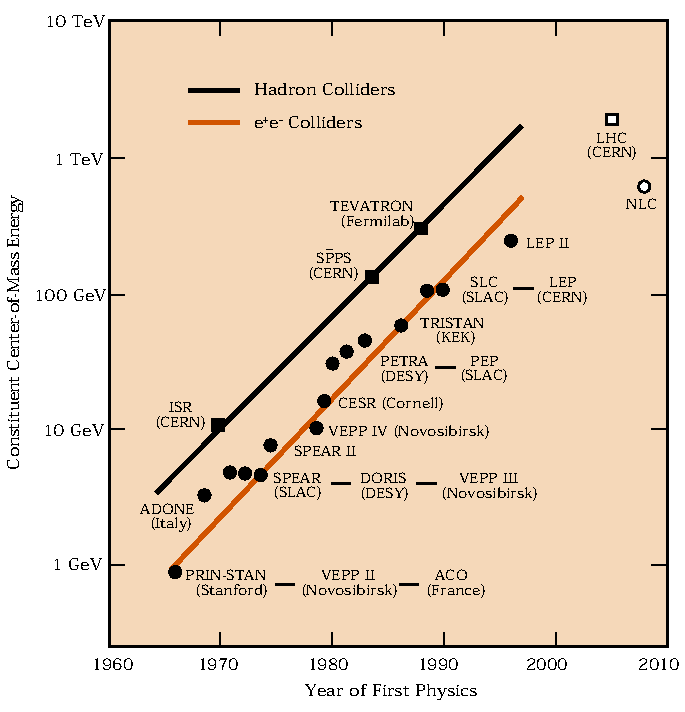
\includegraphics[width=0.5\textwidth]{fig/experiment/ecm_livingston.pdf}
  \caption{
    Plot of the constituent center-of-mass energies for hadronic and $e^+e^-$ colliders since 1960.
    The discovery of massive particles such as the $W$ and $Z$ bosons or the top quark was made possible thanks to advances in accelerator technology that allowed for higher center-of-mass energies and luminosities.
  }
  \label{fig:ECMplot}
\end{figure}

% Chapter overview
This chapter explores the main features of the Large Hadron Collider facility at CERN in section~\ref{sec:LHC}, where collision events used in the search were obtained.
A complete documentation of the LHC machine can be found in reference~\cite{Evans:1129806}.
We then turn our attention to the Compact Muon Solenoid detector in section~\ref{sec:CMS} and briefly go over the main components of the device, which was used to record the collision events at the LHC.
This overview is based off of documents concerning CMS in references~\cite{Chatrchyan:1129810,taylor_2011}.

\section{The Large Hadron Collider}
\label{sec:LHC}

% The Large Hadron Collider
The Large Hadron Collider is a circular collider accelerator facility with two superconducting rings that accelerate protons to relativistic speeds, and it is located just outside of Geneva on the French-Swiss border.
It is the largest and most powerful collider in the world, with plans to extend its service life into the 2030's and 2040's.
It has a circumference of 26.7 km and was built into an existing tunnel that was used for the Large Electron-Positron (LEP) collider, which was used from 1989 to 2000.
Various detectors used to study collision events are placed along the beamline, such as ALICE, ATLAS, CMS, and LHCb.
Figure~\ref{fig:CERN} shows the complete CERN accelerator complex with all of its components~\cite{Mobs:2636343}.
The ATLAS and CMS facilities are general-purpose detectors for studying the Higgs and searching new physics arising from proton collisions, while ALICE is optimized for studying heavy-ion collisions with stripped lead ions ($^{208}$Pb$^{82+}$) to investigate properties of quark-gluon plasma, and LHCb is designed to study the physics of bottom quarks and $CP$ violation in $b$-hadron interactions.

\begin{figure}[htbp]
  \centering
  \includegraphics[width=0.825\textwidth]{fig/experiment/CCC-v2018-print-v2.pdf}
  \caption{
    Layout of the CERN accelerator complex.
    The LHC is one of several accelerators present at the facility, with multiple detectors along the beamline such as ATLAS, CMS, ALICE, and LHCb.
    ATLAS and CMS are both general-purpose detectors for studying properties of the Higgs and searching for new physics.
    ALICE is designed to study heavy-ion collisions with lead ions to investigate quark-gluon plasma.
    LHCb is meant to study the physics of bottom quarks and $CP$ violation in $b$-hadron interactions.
    The LHC is injected with protons and lead ions through a multi-stage process.
    Protons starting at the Linac2 facility, which are then fed through the Proton Synchrotron Booster (PSB), then to the Proton Synchrotron (PS), and then to the Super Proton Synchrotron (SPS) before finally being injected into the LHC itself.
    The lead ions undergo a similar process, starting at Linac3 and then being transferred to the Low Energy Ion Ring (LEIR), then going through the PS and SPS before being injected into the LHC.
  }
  \label{fig:CERN}
\end{figure}

% Beam injection for LHC
The LHC beam is fed through a multi-stage process in which protons are stripped off of hydrogen atoms and are first accelerated through a series of preaccelerators before being injected into the LHC beam.
Protons start at the Linac2 facility, where they are initially accelerated to $50\unit{MeV}$ before being transferred to the Proton Synchrotron Booster (PSB) and reach $1.4\unit{GeV}$.
They are then sent to the Proton Synchrotron (PS) where they reach energies of $25\unit{GeV}$, and then they are accelerated further to $450\unit{GeV}$ at the Super Proton Synchrotron (SPS).
The protons then reach the LHC where they are accelerated to $6.5\unit{TeV}$ each.
The process is similar for lead ions, where they instead start at Linac3 with $4.2\unit{MeV/n}$, then move through the Low Energy Ion Ring (LEIR) before being transferred to the PS, then the SPS, then injected into the LHC.

% Center-of-mass energy and luminosity
While the LHC was built with the intent of achieving center-of-mass energies of $\sqrt{s}=14\unit{TeV}$ in proton collisions, the data collected for this work was over a period in which the center-of-mass energy was $\sqrt{s}=13\unit{TeV}$.
It also has a specific expression for the luminosity $\mathcal{L}$ given by
\begin{equation}
  \mathcal{L}=\frac{N_b^2n_bf_\mathrm{rev}\gamma_r}{4\pi\epsilon_n\beta^*}F,
\end{equation}
where $N_b$ is the number of particles per bunch, $n_b$ is the number of bunches per beam, $f_\mathrm{rev}$ is the revolution frequency, $\gamma_r$ is the Lorentz factor, $\epsilon_n$ is the normalized transverse beam emittance, $\beta^*$ is the beta function at the collision point, and $F$ is the geometric luminosity reduction factor.
The LHC is designed to reach a luminosity of $10^{34}\unit{cm^{-2}s^{-1}}$, but surpassed this value in June 2016~\cite{LHClumi}.
Figure~\ref{fig:CMSlumi} shows the integrated luminosities as a function of time delivered to the CMS detector for the years 2015-2018~\cite{CMSlumi}.
Both ATLAS and CMS are the main high luminosity experiments, with integrated luminosities of $41.0\unit{fb^{-1}}$, $49.8\unit{fb^{-1}}$, and $67.9\unit{fb^{-1}}$ delivered to CMS over the Run 2 years of 2016, 2017, and 2018 respectively.
This corresponds to a total integrated luminosity of $158.7\unit{fb^{-1}}$ at CMS over Run 2.

% Need to check where luminosity figures used in analysis come from
%Both ATLAS and CMS are the main high luminosity experiments, with integrated luminosities of $35.9\unit{fb^{-1}}$, $41.5\unit{fb^{-1}}$, and $59.7\unit{fb^{-1}}$ recorded at CMS over the Run 2 years 2016, 2017, and 2018 respectively.
%This corresponds to a total integrated luminosity of $137.1\unit{fb^{-1}}$ at CMS over Run 2.

\begin{figure}[htbp]
  \centering
  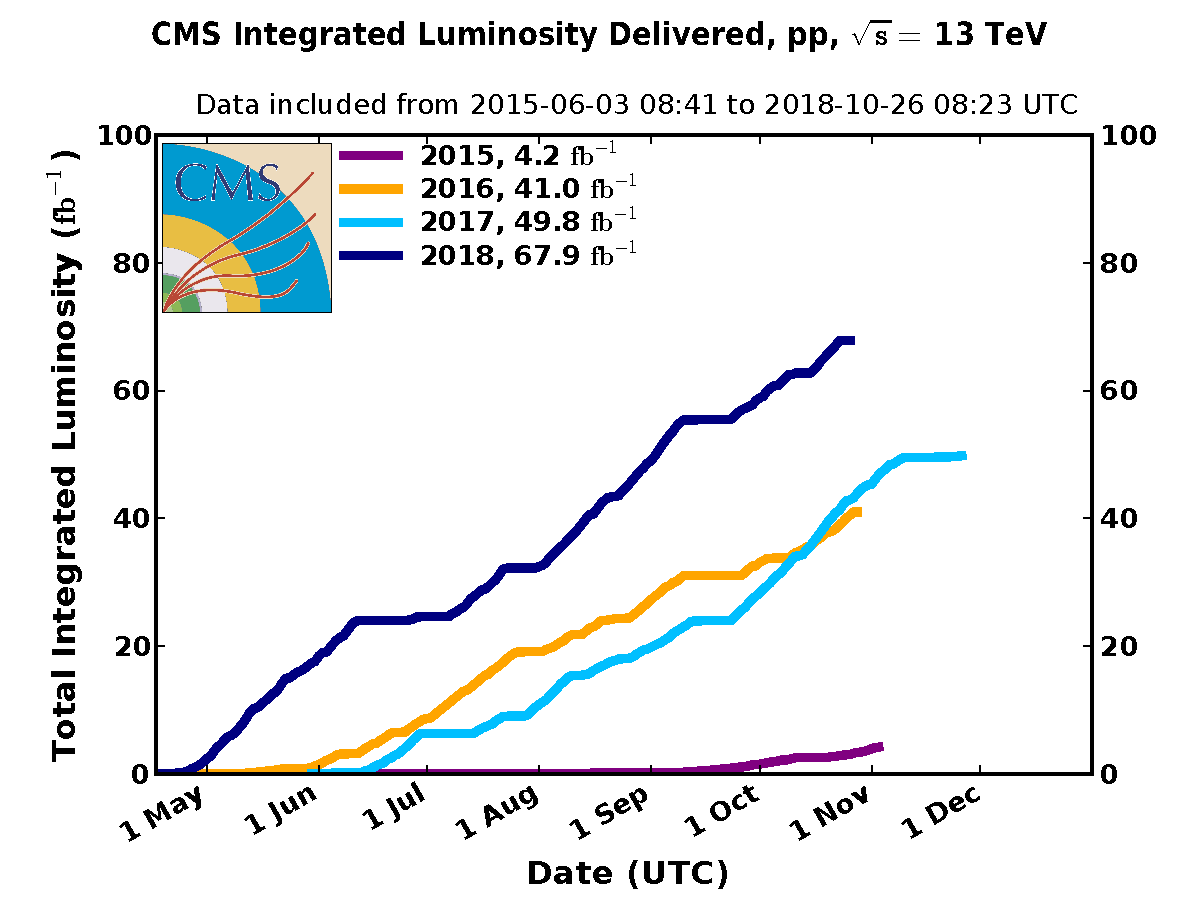
\includegraphics[width=0.65\textwidth]{fig/experiment/int_lumi_cumulative_pp_2_run2.pdf}
  \caption{
    Integrated luminosities delivered to CMS as a function of time for the years 2015-2018.
    This corresponds to a total integrated luminosity of $158.7\unit{fb^{-1}}$ delivered to CMS during the Run 2 years of 2016-2018.
  }
  \label{fig:CMSlumi}
\end{figure}

\section{The Compact Muon Solenoid}
\label{sec:CMS}

% The Compact Muon Solenoid
The Compact Muon Solenoid is one of the main general-purpose detectors at the LHC, and it along with ATLAS obtained independent results for the discovery of the Higgs boson in 2012.
The CMS detector is located 100 meters underground on the French side of the border near the village of Cessy.
It is a cylindrical apparatus with a solenoidal magnet that is coaxial with the beamline of the LHC, with a diameter of $14.6\unit{m}$ and a length of $21.6\unit{m}$, and it is surrounded by various detection systems.
The coordinate system used by CMS is defined such that $z$-axis is defined to lie along the LHC beam, with the $y$-axis pointing vertically upward and the $x$-axis pointing radially inward.
This leads to the azimuthal angle $\phi$ being measured from the $x$-axis in the $x$-$y$ plane, with the radial coordinate denoted by $r$.
The polar angle $\theta$ is defined with respect to the $z$-axis, but in practice one typically uses pseudorapidity defined by $\eta=-\ln\tan(\theta/2)$.

% Function and design overview
One of its primary functions is to accurately identify the charge and momentum of muons emerging from collision events as their trajectories are bent through the magnetic field.
Muons are ideal for reconstructing collisions due to their relatively long lifetime ($\tau_\mu=2.2\unit{\micro s}$), large mass ($m_\mu=105.7\unit{MeV/\clight^2}$), and low radiation losses when propagating through matter~\cite{peskin2019}.
This makes muons the most penetrative and easily identifiable charged particles that can be found in collision events. % Check wording
In addition to identifying muons, the CMS detector also has other components for detecting electrons, photons, and hadrons.
These detection systems are designed in order to meet the demands that come with the LHC's high luminosity, as there are more than 20 proton interactions every $25\unit{ns}$, which results in around 1000 particles emerging for each bunch crossing. % Check numbers
A cutaway diagram of the detector with various components labeled may be seen in figure~\ref{fig:CMScut}~\cite{Sakuma:2665537}.

\begin{figure}[htbp]
  \centering
  \includegraphics[width=0.85\textwidth]{fig/experiment/cms_cutaway.pdf}
  \caption{
    Cutaway diagram of the CMS detector with components labeled as configured in 2018 for Run 2.
    The detector and its components are coaxial with the LHC beam and give wide geometric coverage over the interaction point where the collisions are produced.
    The silicon tracker is used to measure the initial trajectories of charged particles emerging from collisions.
    Outside of the tracker is the preshower detector that screens neutral pions and the electromagnetic calorimeter for detecting electrons and photons.
    The electromagnetic calorimeter is encased by the hadronic calorimeter, which detects hadron jets and neutrinos or exotic particles through missing transverse energy.
    Both calorimeters are surrounded by the muon detection chambers embedded within the return yoke that are used to identify muon charges and momenta.
    Finally, the Cerenkov-based forward calorimeter has both an electromagnetic and hadronic section, lying just outside of the endcaps for the muon chambers. % Check wording
  }
  \label{fig:CMScut}
\end{figure}

% Details on solenoid
One of the central components of the detector is the superconducting solenoid, a $13\unit{m}$ long and $6\unit{m}$ inner diameter magnet that provides a $4\unit{T}$ magnetic field for bending charged particles while operating at a temperature of $4.45\unit{K}$.
The field generated by the solenoid has a nominal current of $19.14\unit{kA}$, an inductance of $14.2\unit{H}$, and a stored energy of $2.6\unit{GJ}$.
The solenoid is supplemented by a $12,500\unit{t}$ flux return yoke that pulls the magnetic field lines back into the muon chambers to allow for high resolution detection of muons produced in collision events.
There are five wheels and two endcaps that comprise this return yoke, with four layers of detection chambers in both the wheels and the endcaps.

\subsection{Inner Tracking System}
\label{subsec:tracking}

% The inner tracker
The inner tracking system measures the momenta of charged particles emerging from collisions and is used to reconstruct secondary vertices for events.
One of the key aspects of the tracking system is the need to choose a design that results in minimal energy loss in charged particles passing through the detector, as this is needed to retain an accurate measurement of their trajectories. % Check wording
Additionally, in order to meet the demands that come with the severe radiation damage that occurs from the large particle flux, the need for efficient cooling, and the level of granularity necessary to measure the tracks of charged particles, the tracking system is based entirely on silicon detectors.
The tracker is $5.8\unit{m}$ long and has a diameter of $2.5\unit{m}$, surrounding the interaction point where collisions occur.
It has a pixel detector with three barrel layers that span radii from $4.4\unit{cm}$ to $10.2\unit{cm}$, as well as a silicon strip tracker with ten layers that extends to a radius of about $1.1\unit{m}$.
Both the pixel detector and silicon strip tracker have endcaps that allow for an acceptance of $|\eta|<2.5$.
% Possibly elaborate

\subsubsection{The Pixel Detector}

% The pixel detector
The pixel detector allows for precise tracking and small impact parameter resolution, which is crucial for secondary vertex reconstruction.
It covers a total area of around $1\unit{m^2}$ and is comprised of 66 million pixels.
The detector has very high efficiency in the barrel region, with losses in efficiency starting around $|\eta|>2.1$. % Possibly insert efficiency graph here
Each pixel cell occupies an area of $100\times150\unit{\micro m^2}$, which allows for high track resolution in the $r$-$\phi$ plane and in the $z$ direction.
Figure~\ref{fig:CMSpixel} shows an illustration of the pixel detector~\cite{Collaboration_2010_pixel}.
As charged particles pass through a silicon pixel, they impart energy onto the electrons in the silicon atoms, which ejects the electrons and generates a current that goes into a readout chip attached to the pixel.
Each pixel consumes about $55\unit{\micro W}$ of power, which results in $3.6\unit{kW}$ of power for the entirety of the pixel detector.
To avoid overheating from the power consumption, the pixels are mounted on cooling tubes, with 10 for the barrel and 4 for the two end disks.

\begin{figure}[htbp]
  \centering
  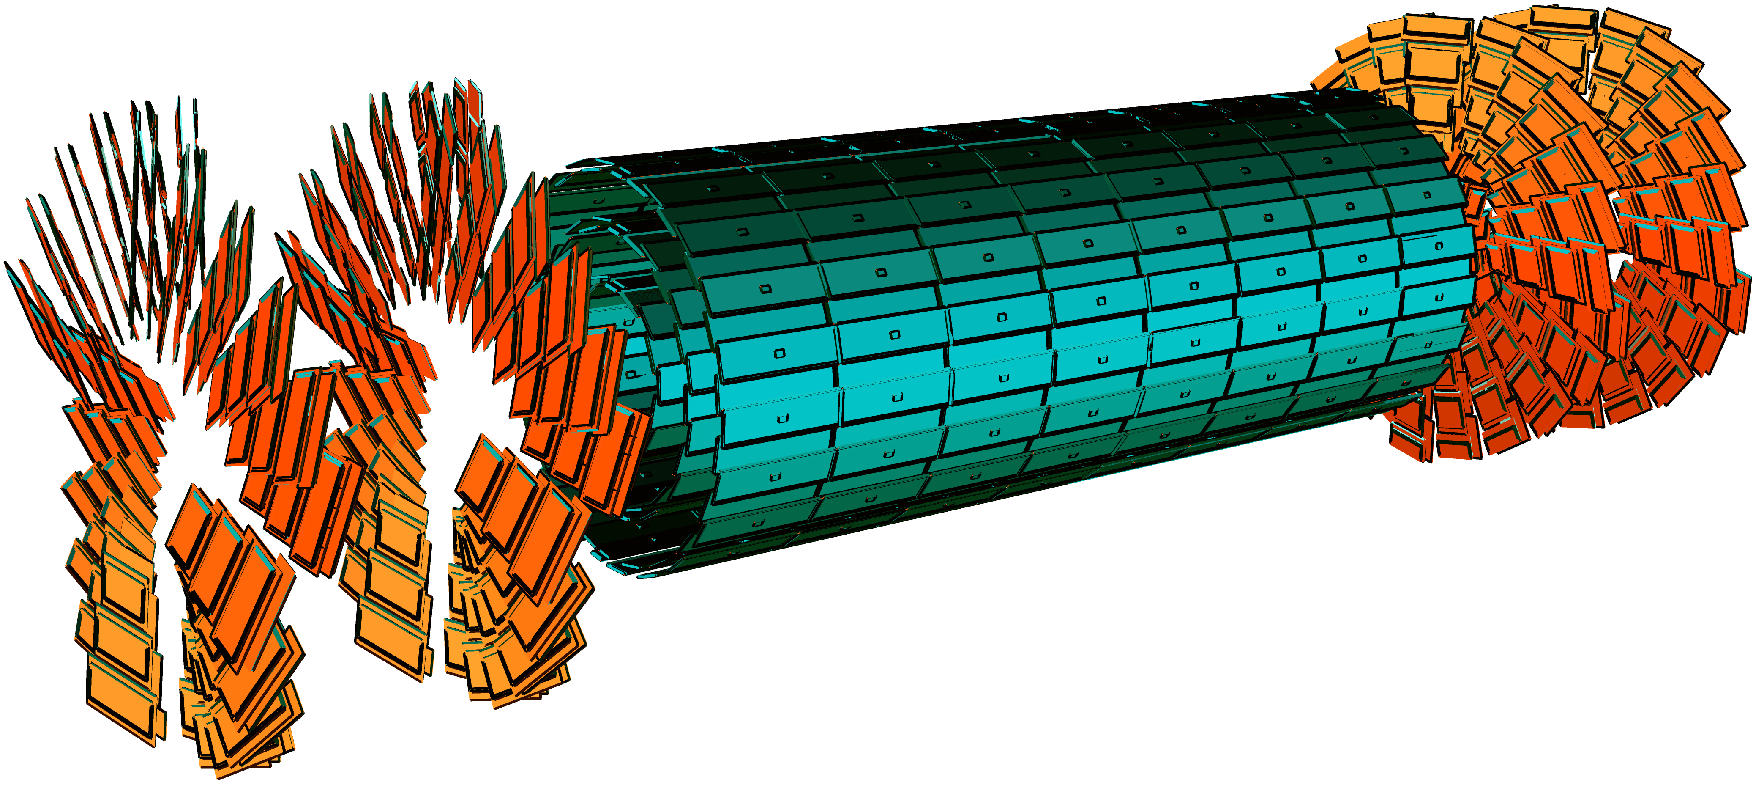
\includegraphics[width=0.85\textwidth]{fig/experiment/cms_pixelTracker.pdf}
  \caption{
    Illustration of the CMS pixel detector, with the barrel region colored in blue, and the endcap regions colored in orange.
    A current is generated as charged particles pass through the pixel cells and eject electrons, which is read by a readout chip attached to each pixel.
  }
  \label{fig:CMSpixel}
\end{figure}

\subsubsection{The Silicon Strip Tracker}

% The silicon strip tracker
Once particles pass through the three layers of the pixel detector, they then go through the silicon strip tracker.
The strip tracker has 15,148 detector modules in total, spread out among several layers, with each module containing 24,244 silicon sensors along with electronic readouts supported by a carbon fiber or graphite frame~\cite{TRK-11-001,Phase1Pixel}.
These strips work in a manner similar to the pixels, with electrons getting knocked out of the material as charged particles pass through them and sending a current to be read out by a sensor.
Figure~\ref{fig:CMSsilicon} shows the layout of the strip tracker~\cite{Chatrchyan:1211825}.
The Tracker Inner Barrel (TIB) has four inner barrel layers of silicon strips placed between radii of $255.0\unit{mm}$ and $498.0\unit{mm}$, which has a length of $1.4\unit{m}$ along the LHC beamline centered at the interaction point.
The TIB is closed off by the Tracker Inner Disks (TID), with the two endcaps containing three disks each placed along the $z$ axis between $\pm800\unit{mm}$ and $\pm900\unit{mm}$ from the interaction point.
The Tracker Outer Barrel (TOB) consists of two double-sided layers of silicon strips just outside the TIB, followed by four single-sided layers, with the layers having radii between $608\unit{mm}$ and $1080\unit{mm}$.
The TOB is closed off by the Tracker EndCaps (TEC) which extend radially from $220\unit{mm}$ to $1135\unit{mm}$ and from $\pm1240\unit{mm}$ to $\pm2800\unit{mm}$ along the beamline.

\begin{figure}[htbp] % Want a higher quality figure
  \centering
  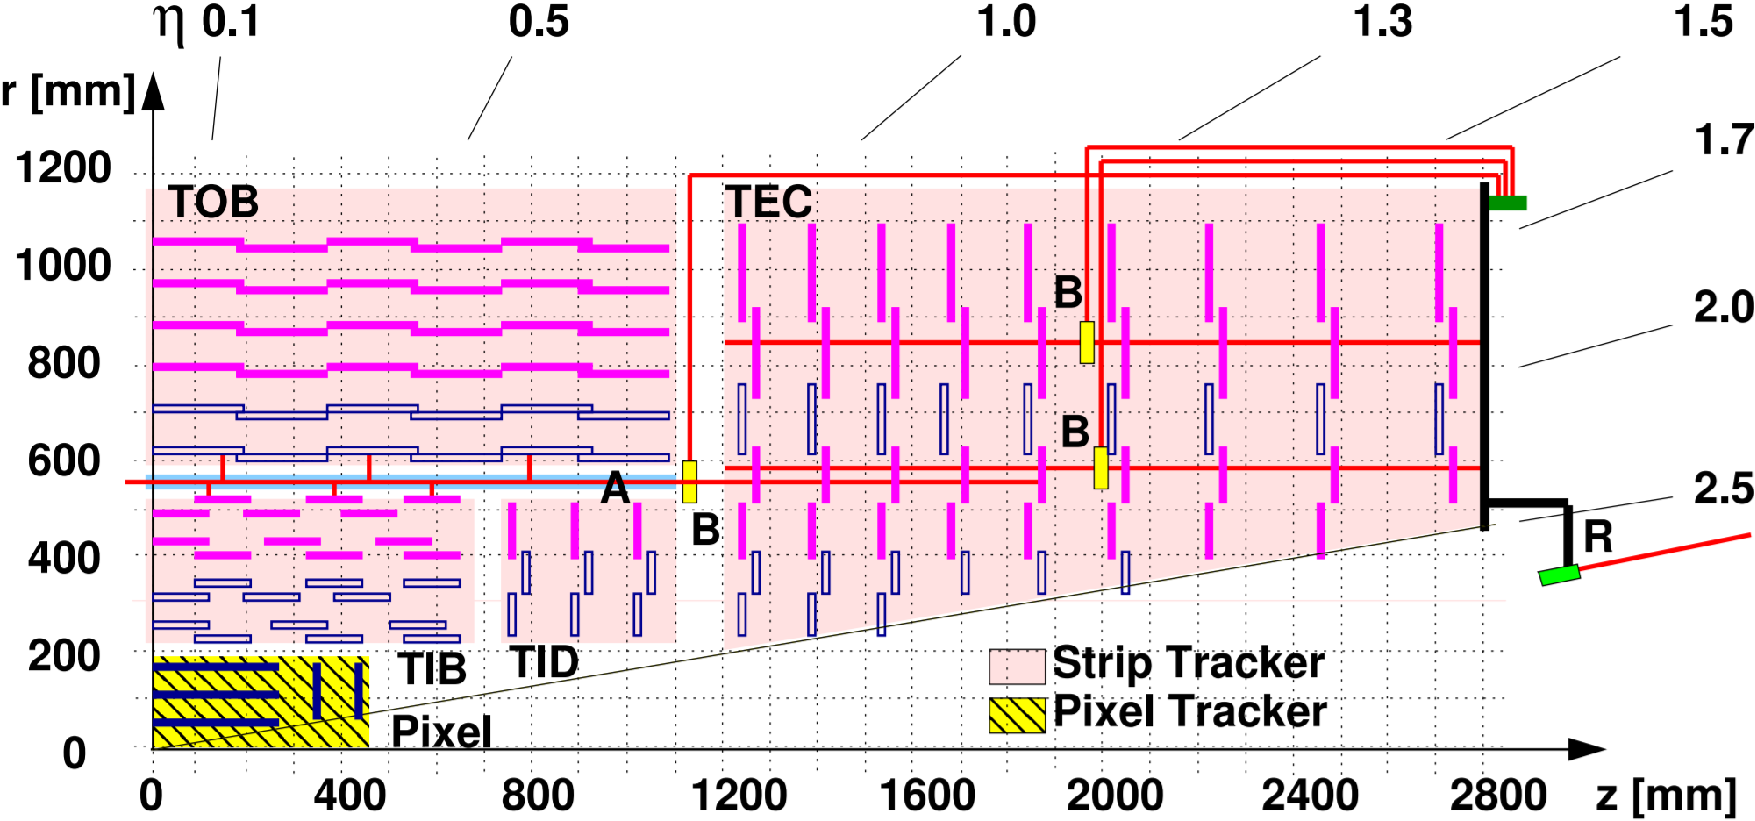
\includegraphics[width=0.85\textwidth]{fig/experiment/cms_siliconTracker.pdf}
  \caption{
    Layout of the CMS silicon strip tracker as seen in the $r$-$z$ plane.
    The Tracker Inner Barrel (TIB) has four inner barrel layers of silicon strips, which is closed off by the Tracker Inner Disks (TID) containing three disks in both of the endcaps.
    The Tracker Outer Barrel (TOB) has two double-sided layers of silicon strips outside of the TIB and is closed off by the Tracker EndCaps (TEC).
  }
  \label{fig:CMSsilicon}
\end{figure}

\subsection{Calorimeters}
\label{subsec:calorimeter}

% The calorimeters
The CMS detector is equipped with various calorimeters that are designed to measure the energies of particles emerging from the collision events.
Unlike the inner tracking system, the calorimeters are designed to abruptly halt any particles passing through them and record the energies of the stopped particles.
The electromagnetic calorimeter (ECAL) and preshower detector lie just outside of the silicon tracker and are designed to detect photons and electrons.
These are both encased by the hadron calorimeter (HCAL), which is used to measure hadron jets and neutrinos or exotic particles that result in missing transverse energy (MET\footnote{Transverse energy is typically written as \Et, which is why missing \Et is abbreviated as MET rather than MTE.}).
Both the ECAL and HCAL are supplemented by the forward calorimeter, which is a Cerenkov-based detector that has electromagnetic and hadronic sections. % Check wording

\subsubsection{Electromagnetic Calorimeter}

% The ECAL
The ECAL consists of 61,200 lead tungstate (PbWO$_4$) crystal scintillators in the barrel region covering the pesudorapidity range $|\eta|<1.479$, with an additional 7,324 crystals in each of the two endcaps to close off the calorimeter.
Figure~\ref{fig:CMSECAL} shows an illustration of a module of the ECAL in the barrel region~\cite{Sakuma_2014}.
Scintillators are materials that emit light after absorbing ionizing radiation, which are attached to a photodetector and generate a current via the photoelectric effect.
These crystals were selected due to their density ($8.28\unit{g/cm^3}$), radiation length ($0.89\unit{cm}$), and Moli\`{e}re radius ($2.2\unit{cm}$), all of which allow for high resolution measurement of electron and photon energies while withstanding the harsh radiation levels of the LHC.
The photodetectors attached to the scintillators are also specially designed to operate in the $4\unit{T}$ magnetic field generated by the solenoid.
Additionally, around 80\% of the light from the scintillation effect is emitted in the LHC bunch crossing time of $25\unit{ns}$, which is adequate for detection purposes.
The crystals measure $22\times22\unit{mm^2}$ at the front face and $26\times26\unit{mm^2}$ at the rear face, corresponding to $0.0174\times0.0174$ in the $\eta$-$\phi$ plane, and have a length of $230\unit{mm}$.

\begin{figure}[htbp]
  \centering
  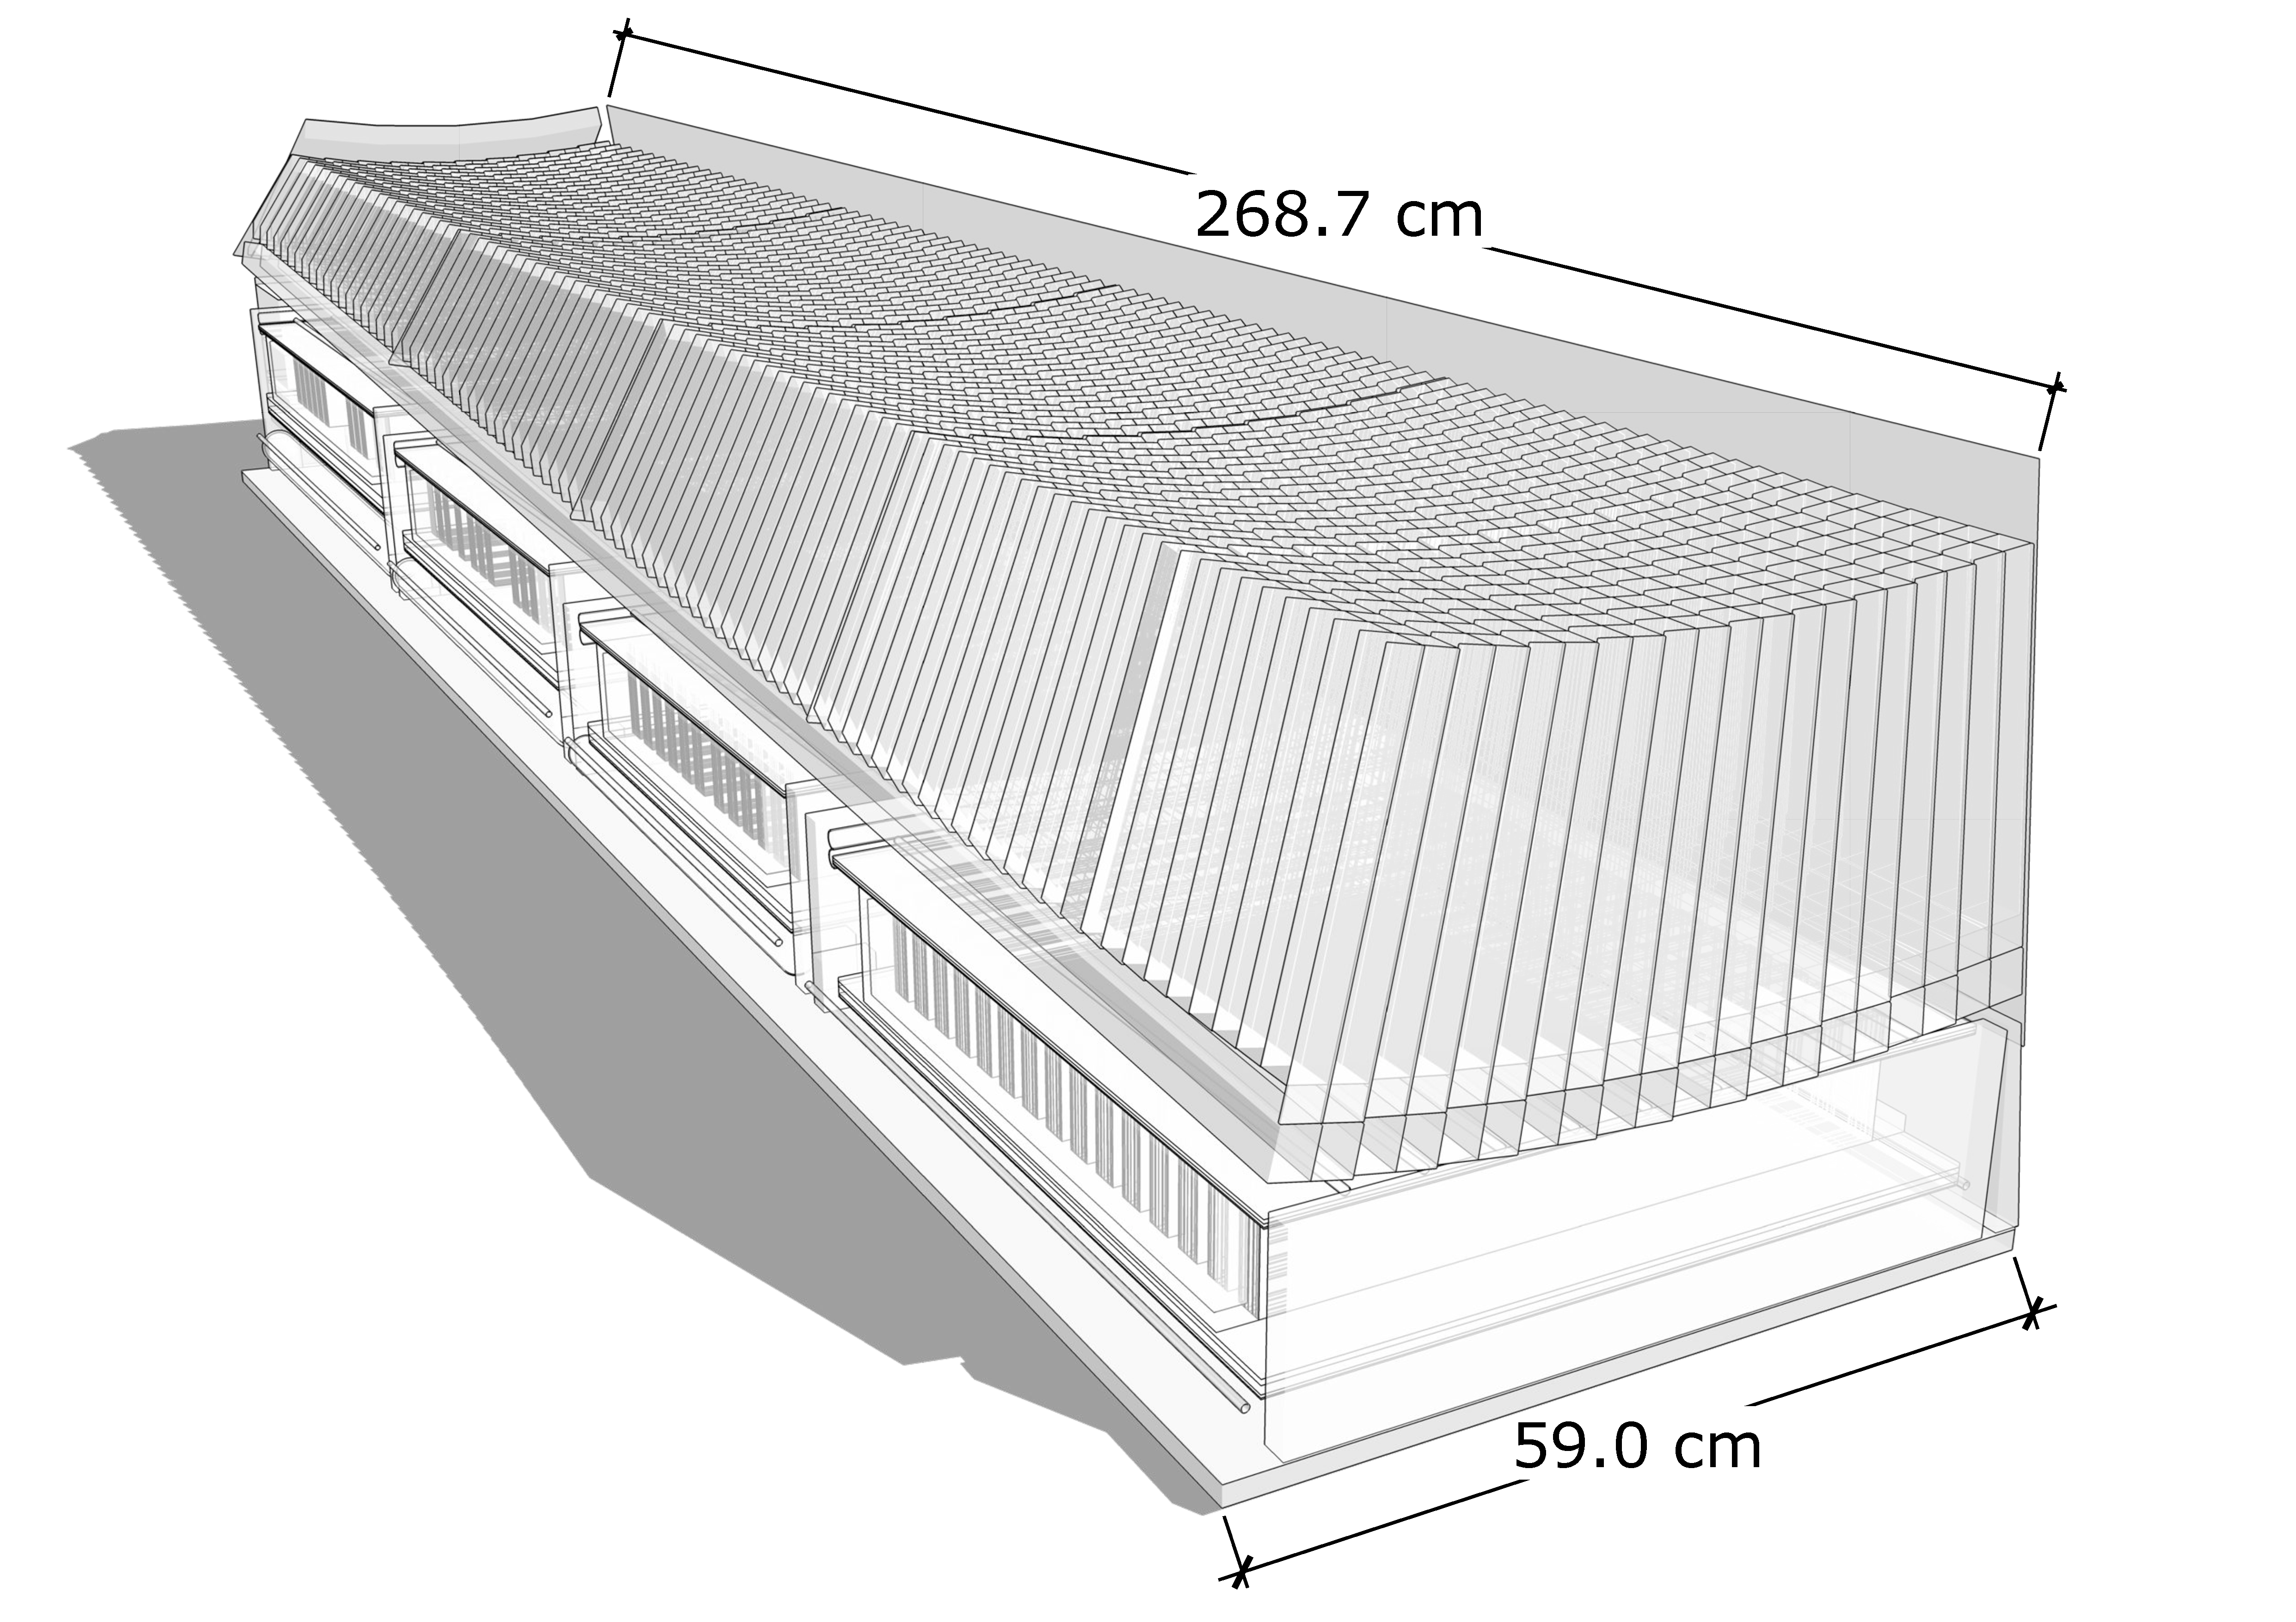
\includegraphics[width=0.65\textwidth]{fig/experiment/20130816_01_EB_module_1.pdf}
  \caption{
    Illustration of a module of the CMS ECAL in the barrel showing the layout of the lead tungstate scintillators.
    The scintillators emit light after absorbing ionizing radiation, each of which are attached to photodetectors and generate a current from the scintillation light.
  }
  \label{fig:CMSECAL}
\end{figure}

% Preshower detector
The ECAL also encloses a preshower detector that is designed to screen out neutral pions, as they can decay into two closely-spaced high-energy photons.
It also helps with identifying electrons against minimum ionizing particles and improves the position resolution for electrons and photons.
The preshower operates in the region $1.653<|\eta|<2.6$, and is closed off by two endcaps.
It is made of two layers, with lead radiators that generate electromagnetic showers when penetrated by incoming photons and electrons, and silicon strip sensors placed after each radiator to measure the deposited energies from the showers.
The detector strips are much finer than that of the ECAL crystals and are $2\unit{mm}$ wide, which allows for distinguishing individual photons from pion decays.

\subsubsection{Hadron Calorimeter}

% The hadron calorimeter
Outside of the ECAL lies the various layers of the HCAL, which is divided into four sections.
Figure~\ref{fig:CMSHCAL} shows the layout of the HCAL~\cite{Collaboration_2010_HCAL}.
The first of these is the barrel (HB), which covers the pseudorapidity range $|\eta|<1.3$.
The HB has 36 azimuthal wedges that are constructed out of brass absorber plates bolted together in a staggered geometry.
Between the layers of brass are tiles of plastic scintillators that cover an area of $0.087\times0.087$ in the $\eta$-$\phi$ plane.
To maximize the coverage of the HCAL and obtain an accurate reading of the deposited energies, the wedges are bolted together so as to allow for no more of a gap than $2\unit{mm}$ between the wedges.
The endcaps (HE) cover the HB section and extend over the pseudorapidity range $1.3<|\eta|<3$.
Scintillators in this region have a granularity of $\Delta\eta\times\Delta\phi=0.087\times0.087$ in the region $|\eta|<1.6$ and $\Delta\eta\times\Delta\phi\approx0.017\times0.017$ for $|\eta|\geq1.6$.
The outer calorimeter (HO) sits just outside of the vacuum tank of the solenoid, divided into five rings aligned along the axis of the LHC beam.
The central ring of the HO has two layers of scintillators at radii of $3.82\unit{m}$ and $4.07\unit{m}$, while the other rings only have a single scintillator layer at $4.07\unit{m}$.
Finally, the forward calorimeter (HF) consists of two detectors that are $11.2\unit{m}$ away from the interaction point on both sides of CMS.
The HF faces the unique challenge of dealing with intense radiation, as most of the energy from the collisions is directed into the forward regions of the detector.
For this reason, quartz fibers were used as the scintillation material and the signal is generated by Cherenkov radiation from charged particles passing through the medium.

\begin{figure}[htbp]
  \centering
  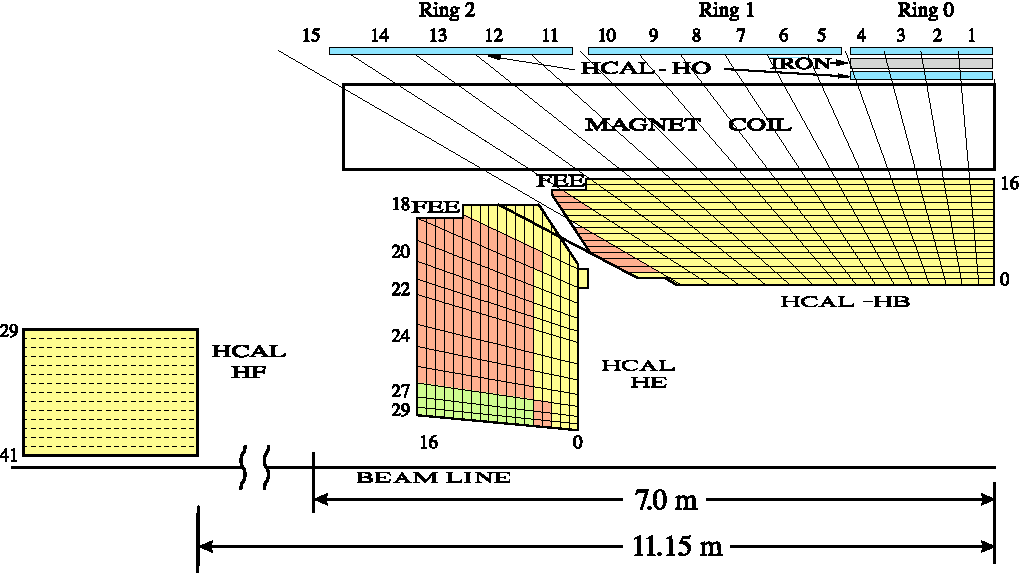
\includegraphics[width=0.75\textwidth]{fig/experiment/HCAL-HB-HE-HO-HF.pdf}
  \caption{
    Layout of the HCAL in the $r$-$z$ plane.
    The HCAL surrounds the ECAL and has four sections denoted by the barrel (HB), endcaps (HE), outer calorimeter (HO), and forward calorimeter (HF).
    The scintillation material in the HB, HE, and HO sections is made of plastic, while the HF section uses quarts fibers in order to withstand the intense radiation in the forward region of the detector.
  }
  \label{fig:CMSHCAL}
\end{figure}

\subsection{Muon Tracking System}
\label{subsec:muonTrack}

% The muon system
The muon system is of central importance to the CMS detector.
From its inception as a detector, it was recognized that muons would be one of the primary tools for reconstructing collision events.
One reason for this is the fact that final states with muons present offer some of the best results for mass resolution, thereby increasing the discovery potential for new physics.
This was one of the considerations taken into account when designing the CMS detector to optimize for the observation of the Higgs before it was discovered.
The so-called $H\to ZZ^{(*)}\to 4\ell$ ``golden channel'' has the cleanest signal when all four of the leptons in the final state are muons~\cite{Gainer_2011}.
Moreover, muons are expected to be produced in many decay events for exotic particles from BSM theories.
As such, the muon system is designed to provide robust and accurate muon identification, momentum measurement, and triggering for events.
This is achieved thanks to the combination of the strong solenoidal magnetic field and the flux return yoke.
The return yoke allows for pulling the magnetic field lines from the solenoid to the outer region where the muon detection chambers are located, and it also screens out hadrons by absorbing them.
The detection hits in the layers of the muon chambers then allow for reconstructing the charge and momentum of the muons.

% Detection chambers
There are three kinds of gaseous detection chambers that are used to identify and measure muons: drift tubes (DTs), cathode strip chambers (CSCs), and resistive plate chambers (RPCs).
The outer region of CMS has 250 DTs in the barrel region covering pseudorapidities of $|\eta|<1.2$, while the endcaps on both ends of CMS have 540 CSCs covering the region $0.9<|\eta|<2.4$.
The RPCs are distributed throughout both regions of CMS, with 480 in the barrel and 576 in the endcaps.
In total, there are 1846 muon chambers present on the detector, with the chambers distributed among four layers in both the barrel and endcap regions to allow for track reconstruction. % Check numbers
The barrel region is split up into five concentric wheels that are numbered from $-2$ to $+2$, with wheel 0 centered at the interaction point.
Figure~\ref{fig:CMScrosssec} shows a cross section of the CMS detector in the $r$-$z$ plane as configured during Run 2, with DTs, CSCs, and RPCs labeled~\cite{Sirunyan_2018_CMS}.

\begin{figure}[htbp]
  \centering
  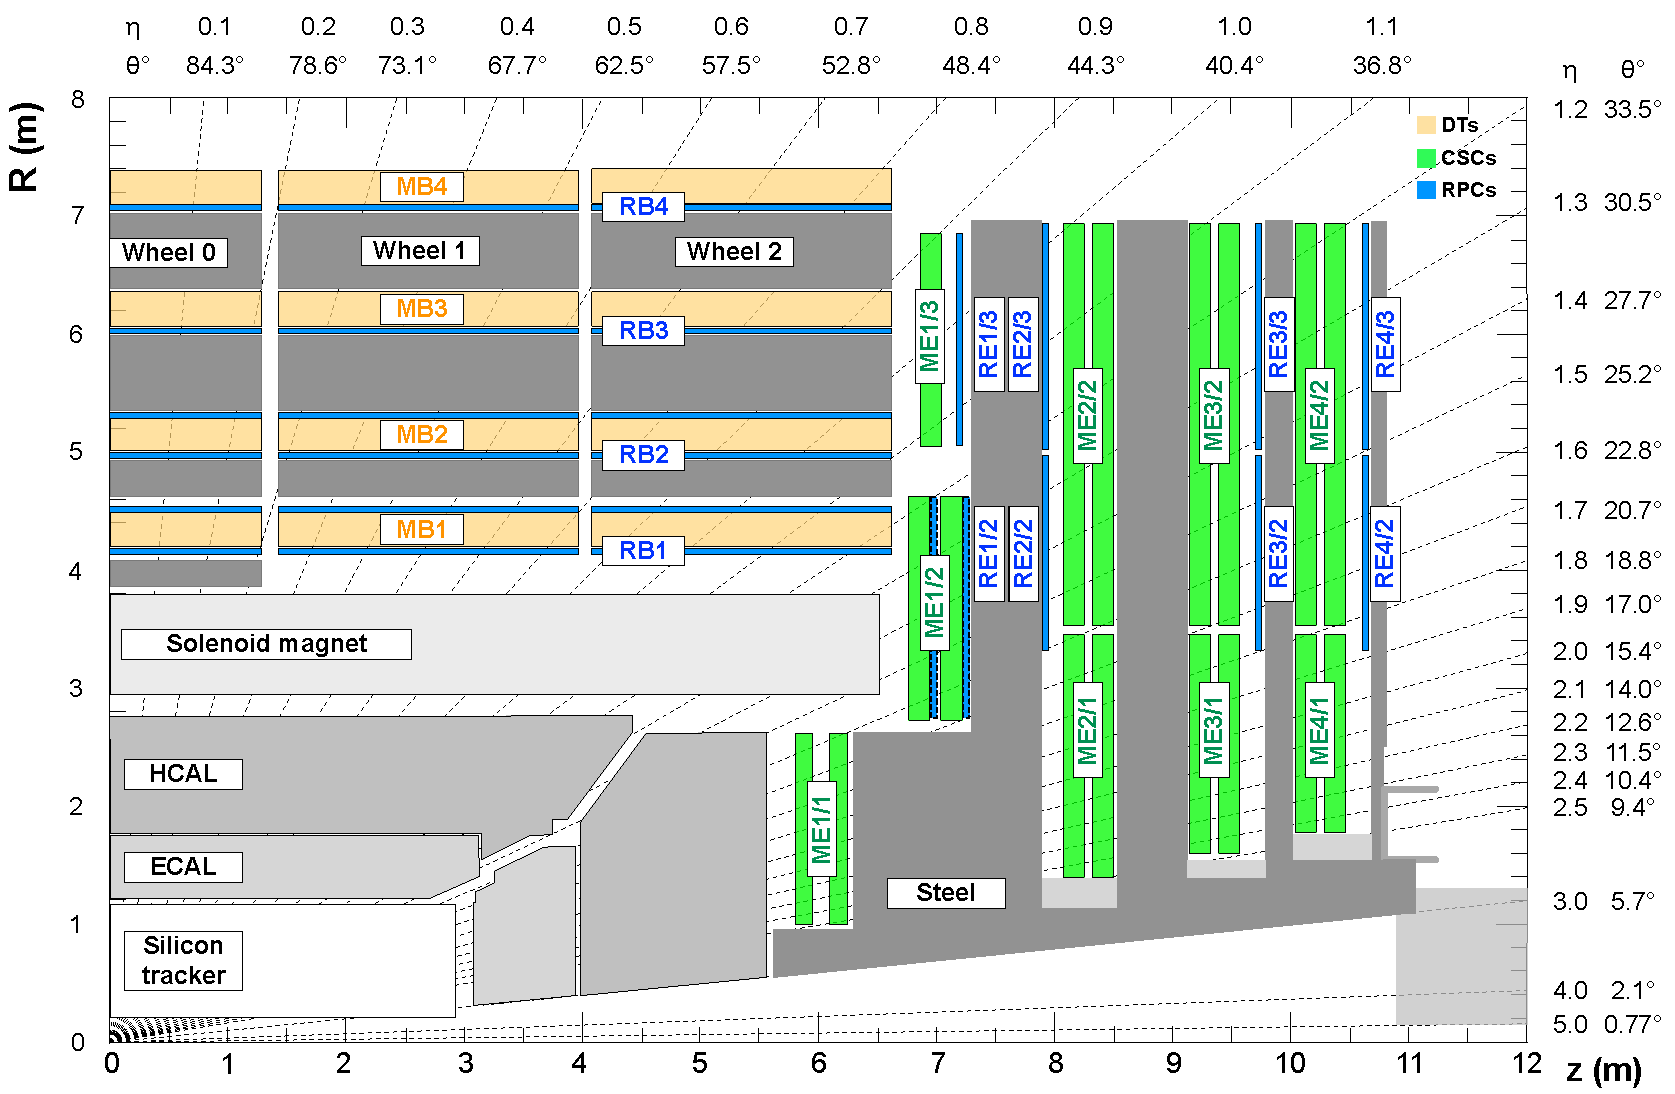
\includegraphics[width=0.85\textwidth]{fig/experiment/cms_crosssec.pdf}
  \caption{
    cross section of the CMS detector in the $r$-$z$ plane as configured during Run 2.
    The barrel region contains a combination of drift tubes and resistive plate chambers distributed among five concentric wheels surrounding the detector, covering a pseudorapidity range of $|\eta|<1.2$.
    The endcaps on either side cover the range $0.9<|\eta|<2.4$, and have combinations of cathode strip chambers and resistive plate chambers present.
    There are 250 drift tubes and 480 resistive plate chambers in the barrel, and 540 cathode strip chambers and 576 resistive plate chambers in the endcaps, making a total of 1846 muon chambers distributed throughout CMS.
    Both the barrel and endcaps have four layers of muon chambers to allow for track reconstruction.
  }
  \label{fig:CMScrosssec}
\end{figure}

\subsubsection{Drift Tubes}

% The DT system
The DT system in the barrel region is distributed among the four layers present in each wheel surrounding the interaction point, with the layers referred to as stations.
The stations are numbered according to how close they are to the interaction point, with station 1 being the innermost layer and station 4 being the outermost.
Each drift tube contains a gaseous mix of Ar (85\%) and CO$_2$ (15\%), with sensitive wires inside of the tubes held at a specified potential.
An illustration of an individual drift tube cell can be seen in figure~\ref{fig:CMSDTcell}~\cite{Abbiendi_2019}.
As muons pass through the gas, they impart enough ionization energy to knock off electrons from the atoms of the gas, which are then attracted to the wire and cause a cascade of additional electrons from the gas to be deposited onto the wire and cause a current.
The muon's position can then be inferred from where the electrons hit the wire, and how far the muon was from the wire.
Additionally, the muon track and momentum can be reconstructed by using multiple detection hits from different stations in the barrel.
Each DT allows for a position resolution of $0.25\unit{mm}$.

\begin{figure}[htbp]
  \centering
  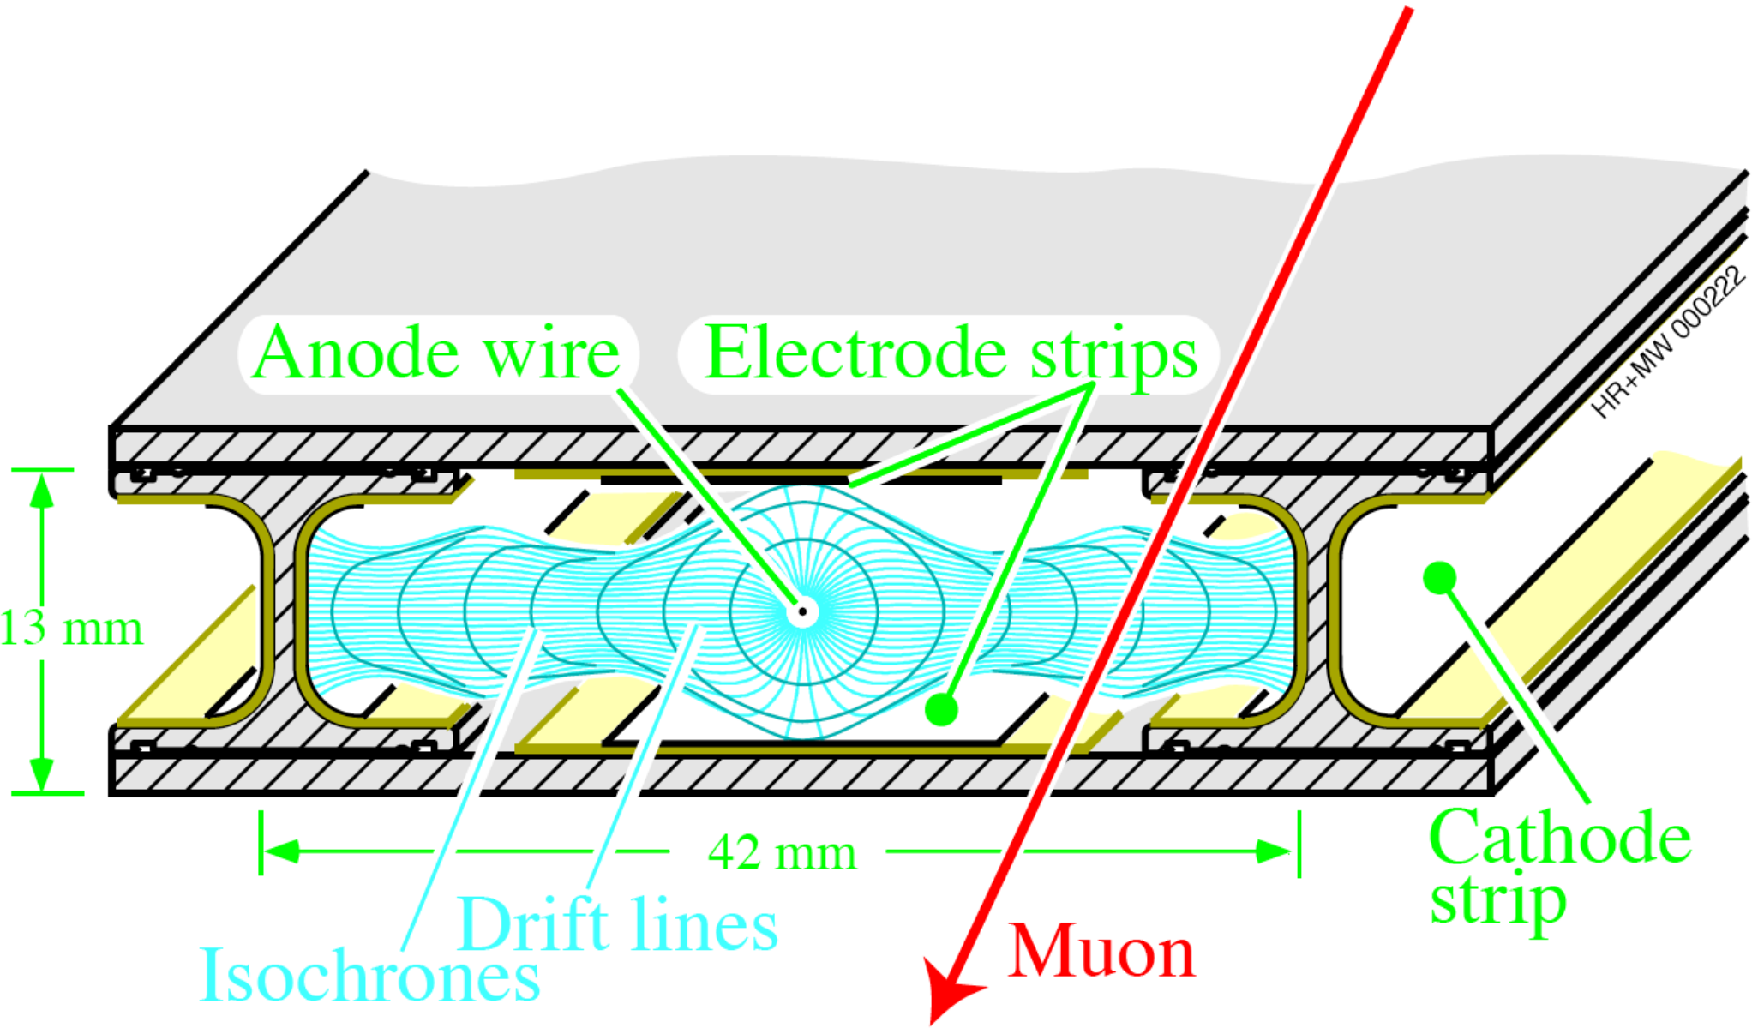
\includegraphics[width=0.65\textwidth]{fig/experiment/cms_DTcell.pdf}
  \caption{
    Illustration of a drift tube cell.
    As muons pass through the cell, they ionize the gas and cause a cascade of electrons that deposit onto the anode wire and generate a current.
    The current is readout by the detector and allows for measuring muon momentum.
  }
  \label{fig:CMSDTcell}
\end{figure}

\subsubsection{Cathode Strip Chambers}

% The CSC system
The CSCs in the endcaps operate under a similar principle to that of the DTs in the barrel region.
They are made of trapezoidal panels and have a gas mix of Ar (40\%), CO$_2$ (50\%), and CF$_4$ (10\%).
Figure~\ref{fig:CMSCSC} shows a cut-away diagram of a CSC chamber~\cite{collaboration_2013}.
Inside of the CSCs are arrays of positively-charged anode wires and negatively-charged cathode copper strips that are perpendicular to each other.
When muons ionize the gas after passing through the chamber, they cause an avalanche of electrons to deposit onto the wire and generate a current, but they also cause an induced charge on the copper strips.
This allows for a precise measurement of $\phi$ for the passing muons and a coarse measurement of $r$ from the anode wires, resulting in a $0.2\unit{mm}$ resolution position measurement, as well as a fast time measurement.

\begin{figure}[htbp]
  \centering
  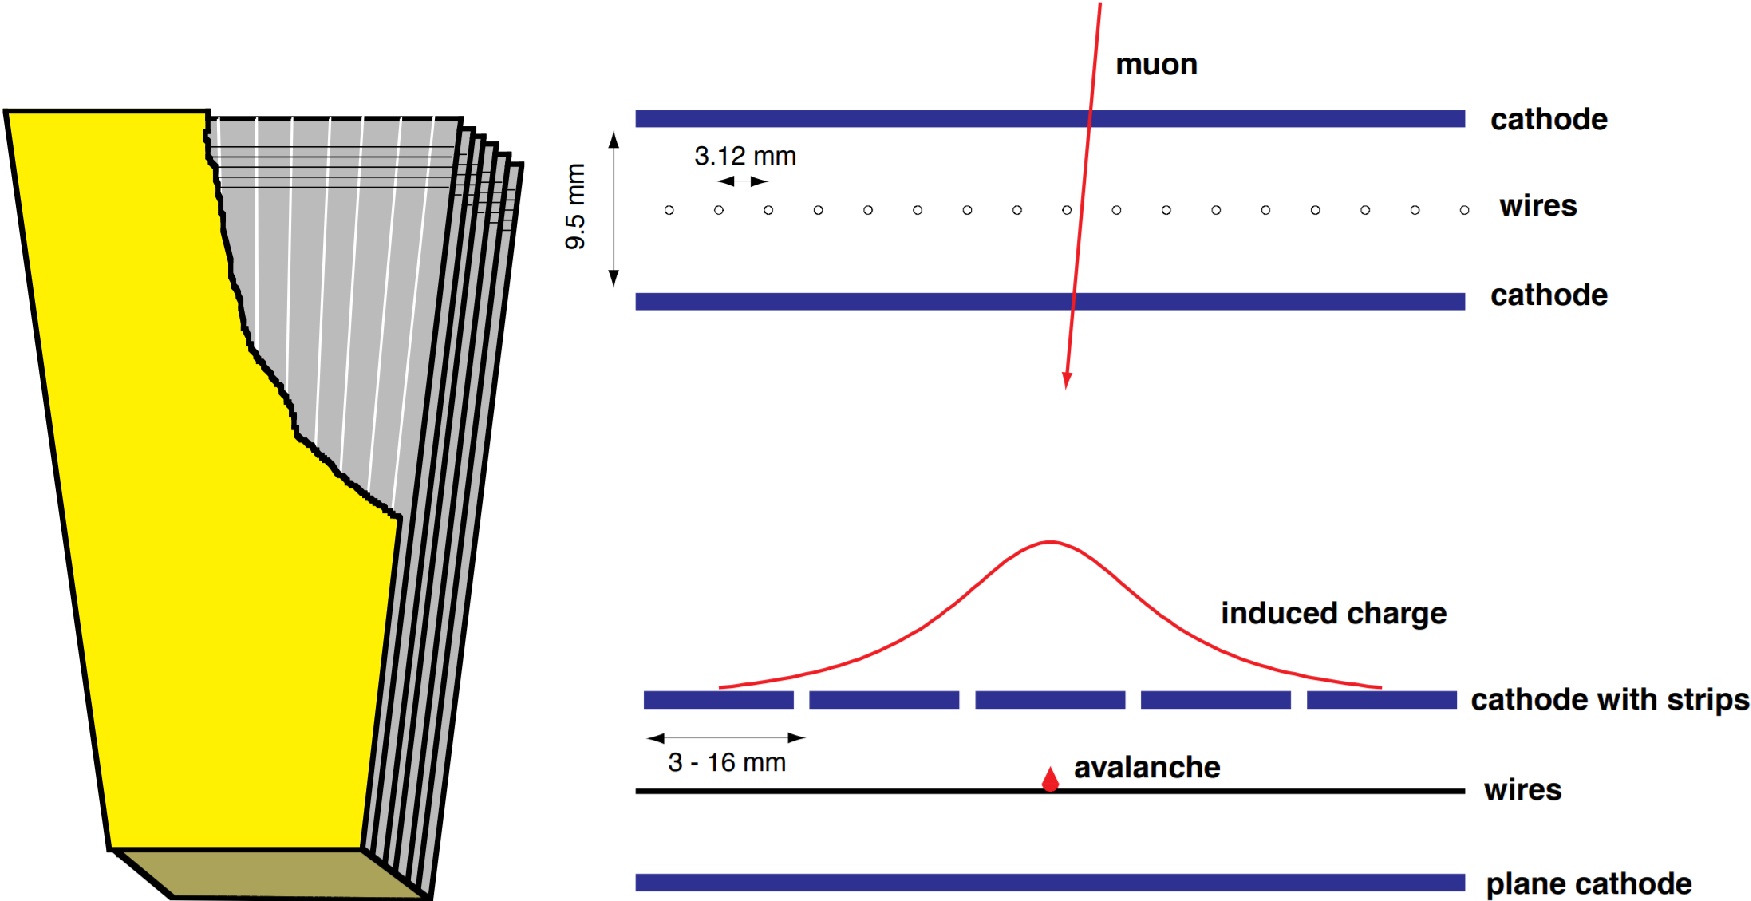
\includegraphics[width=0.75\textwidth]{fig/experiment/cms_csc.pdf}
  \caption{
    Cut-away diagram of a CSC (left) with an illustration of the ionization mechanism (right).
    As muons ionize the gas, the resulting electron avalanche deposits onto the wires and generate a current, while also inducing a charge onto the cathode strips.
    This gives a measurement of the muon position for both $\phi$ and $r$.
  }
  \label{fig:CMSCSC}
\end{figure}

\subsubsection{Resistive Plate Chambers}

% RPCs
RPCs are used to supplement the DTs in the barrel and the CSCs in the endcaps.
They are gaseous detectors that consist of two parallel plastic plates with high resistivity, one being a positively-charged anode and the other a negatively-charged cathode.
Figure~\ref{fig:CMSRPC} shows an example of a double gap RPC design~\cite{kumari2020improvedrpc}.
The gaseous mix in the RPCs is C$_2$H$_2$F$_4$ (95.2\%), isoC$_4$H$_{10}$ (4.5\%), and SF$_6$ (0.3\%).
The electron cascade caused by the ionization of a passing muon generates a signal on external detecting strips, which allows for a coarse spatial measurement, but a very fast time measurement ($1\unit{ns}$) that is shorter than the $25\unit{ns}$ between each bunch crossing.
Their fast response time is used in the trigger system in order to determine whether or not event data should be saved based on the measured muon momentum.

\begin{figure}[htbp]
  \centering
  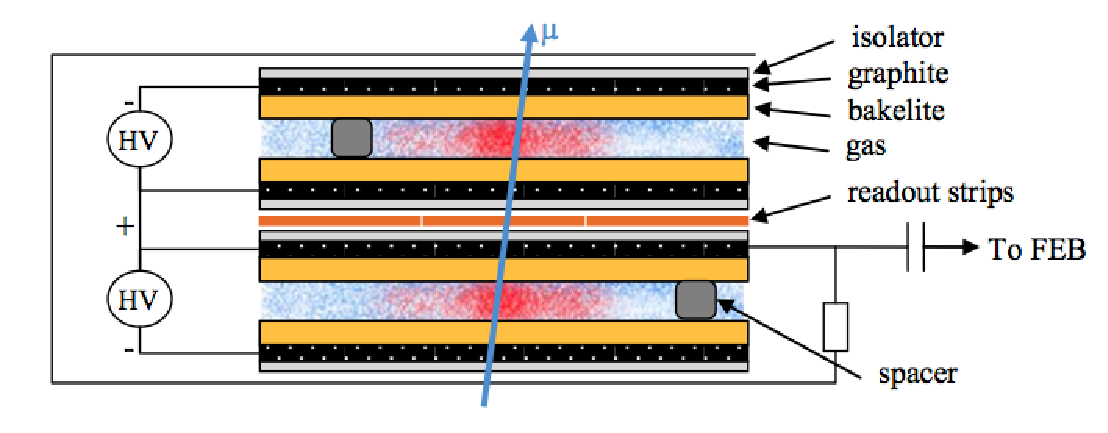
\includegraphics[width=0.65\textwidth]{fig/experiment/rpc_schema.pdf}
  \caption{
    Illustration of a double gap RPC design.
    The electron cascade generated by the ionization process induces a signal on the readout strips, which gives a coarse spatial measurement.
    DTs and CSCs are supplemented by RPCs that are used by the trigger system due to their fast response time.
  }
  \label{fig:CMSRPC}
\end{figure}

\subsection{Trigger System}
\label{subsec:trigger}

% Motivation for the trigger system
One of the unique challenges facing detectors at the LHC is the large amount of collision events that occur at the interaction points.
proton collisions occur every $25\unit{ns}$, corresponding to a rate of $40\unit{MHz}$.
With 20 simultaneous $pp$ collisions for every bunch crossing, this corresponds to $8\times10^8$ interactions every second.
It is not possible to meet the hardware demands for recording every single collision event, nor would it be prudent to do so since most events are soft collisions between protons that do not reveal any new physics.
Thus, the trigger system is needed in order to select for high-energy events of interest, while also recording them at a reasonable rate that allows for long-term storage.

% Trigger system overview
The trigger system has two levels, consisting of a Level-1 (L1) Trigger, and a High-Level Trigger (HLT)~\cite{CMStrigger}.
The L1 Trigger is hardware-based and is comprised of custom-designed electronics that uses data from the calorimeters and muon system.
The HLT is software-based and consists of a conventional CPU farm, which has access to a complete readout from the L1 Trigger and is able to perform more advanced calculations with the data.
The trigger system as whole reduces the rate by a factor of $10^6$, with the L1 Trigger designed to have an output rate of 100 kHz.
In practice, the L1 Trigger is not operated at its maximum output and instead runs at 30 kHz as a safety measure.

\subsubsection{Level-1 Trigger}

% Level 1 trigger
The architecture of the L1 trigger can be seen in figure~\ref{fig:L1Trigger}~\cite{cmscollaboration2020performance}.
At the local level, the L1 Trigger consists of Trigger Primitive Generators (TPG) that are activated by track segments or hit patterns in muon chambers, and energy deposits in the calorimeters.
The trigger primitives are then used by the Regional Triggers to form trigger objects for candidate particles, such as electrons, photons, and muons.
These objects have to be ranked and sorted based on their energy, momenta, and quality.
The highest rank objects are then transferred to the Global Trigger and are evaluated to determine whether or not they will be passed onto the HLT.
This is determined by the Trigger Control System (TCS), which will then pass a Level-1 Accept (L1A) decision back to the Global Trigger.
The allowed latency between the a single bunch crossing and the L1A decision in the L1 Trigger is $3.2\unit{\micro s}$, which requires the entire process to be pipelined so that the L1 Trigger may operate continuously.

\begin{figure}[htbp]
  \centering
  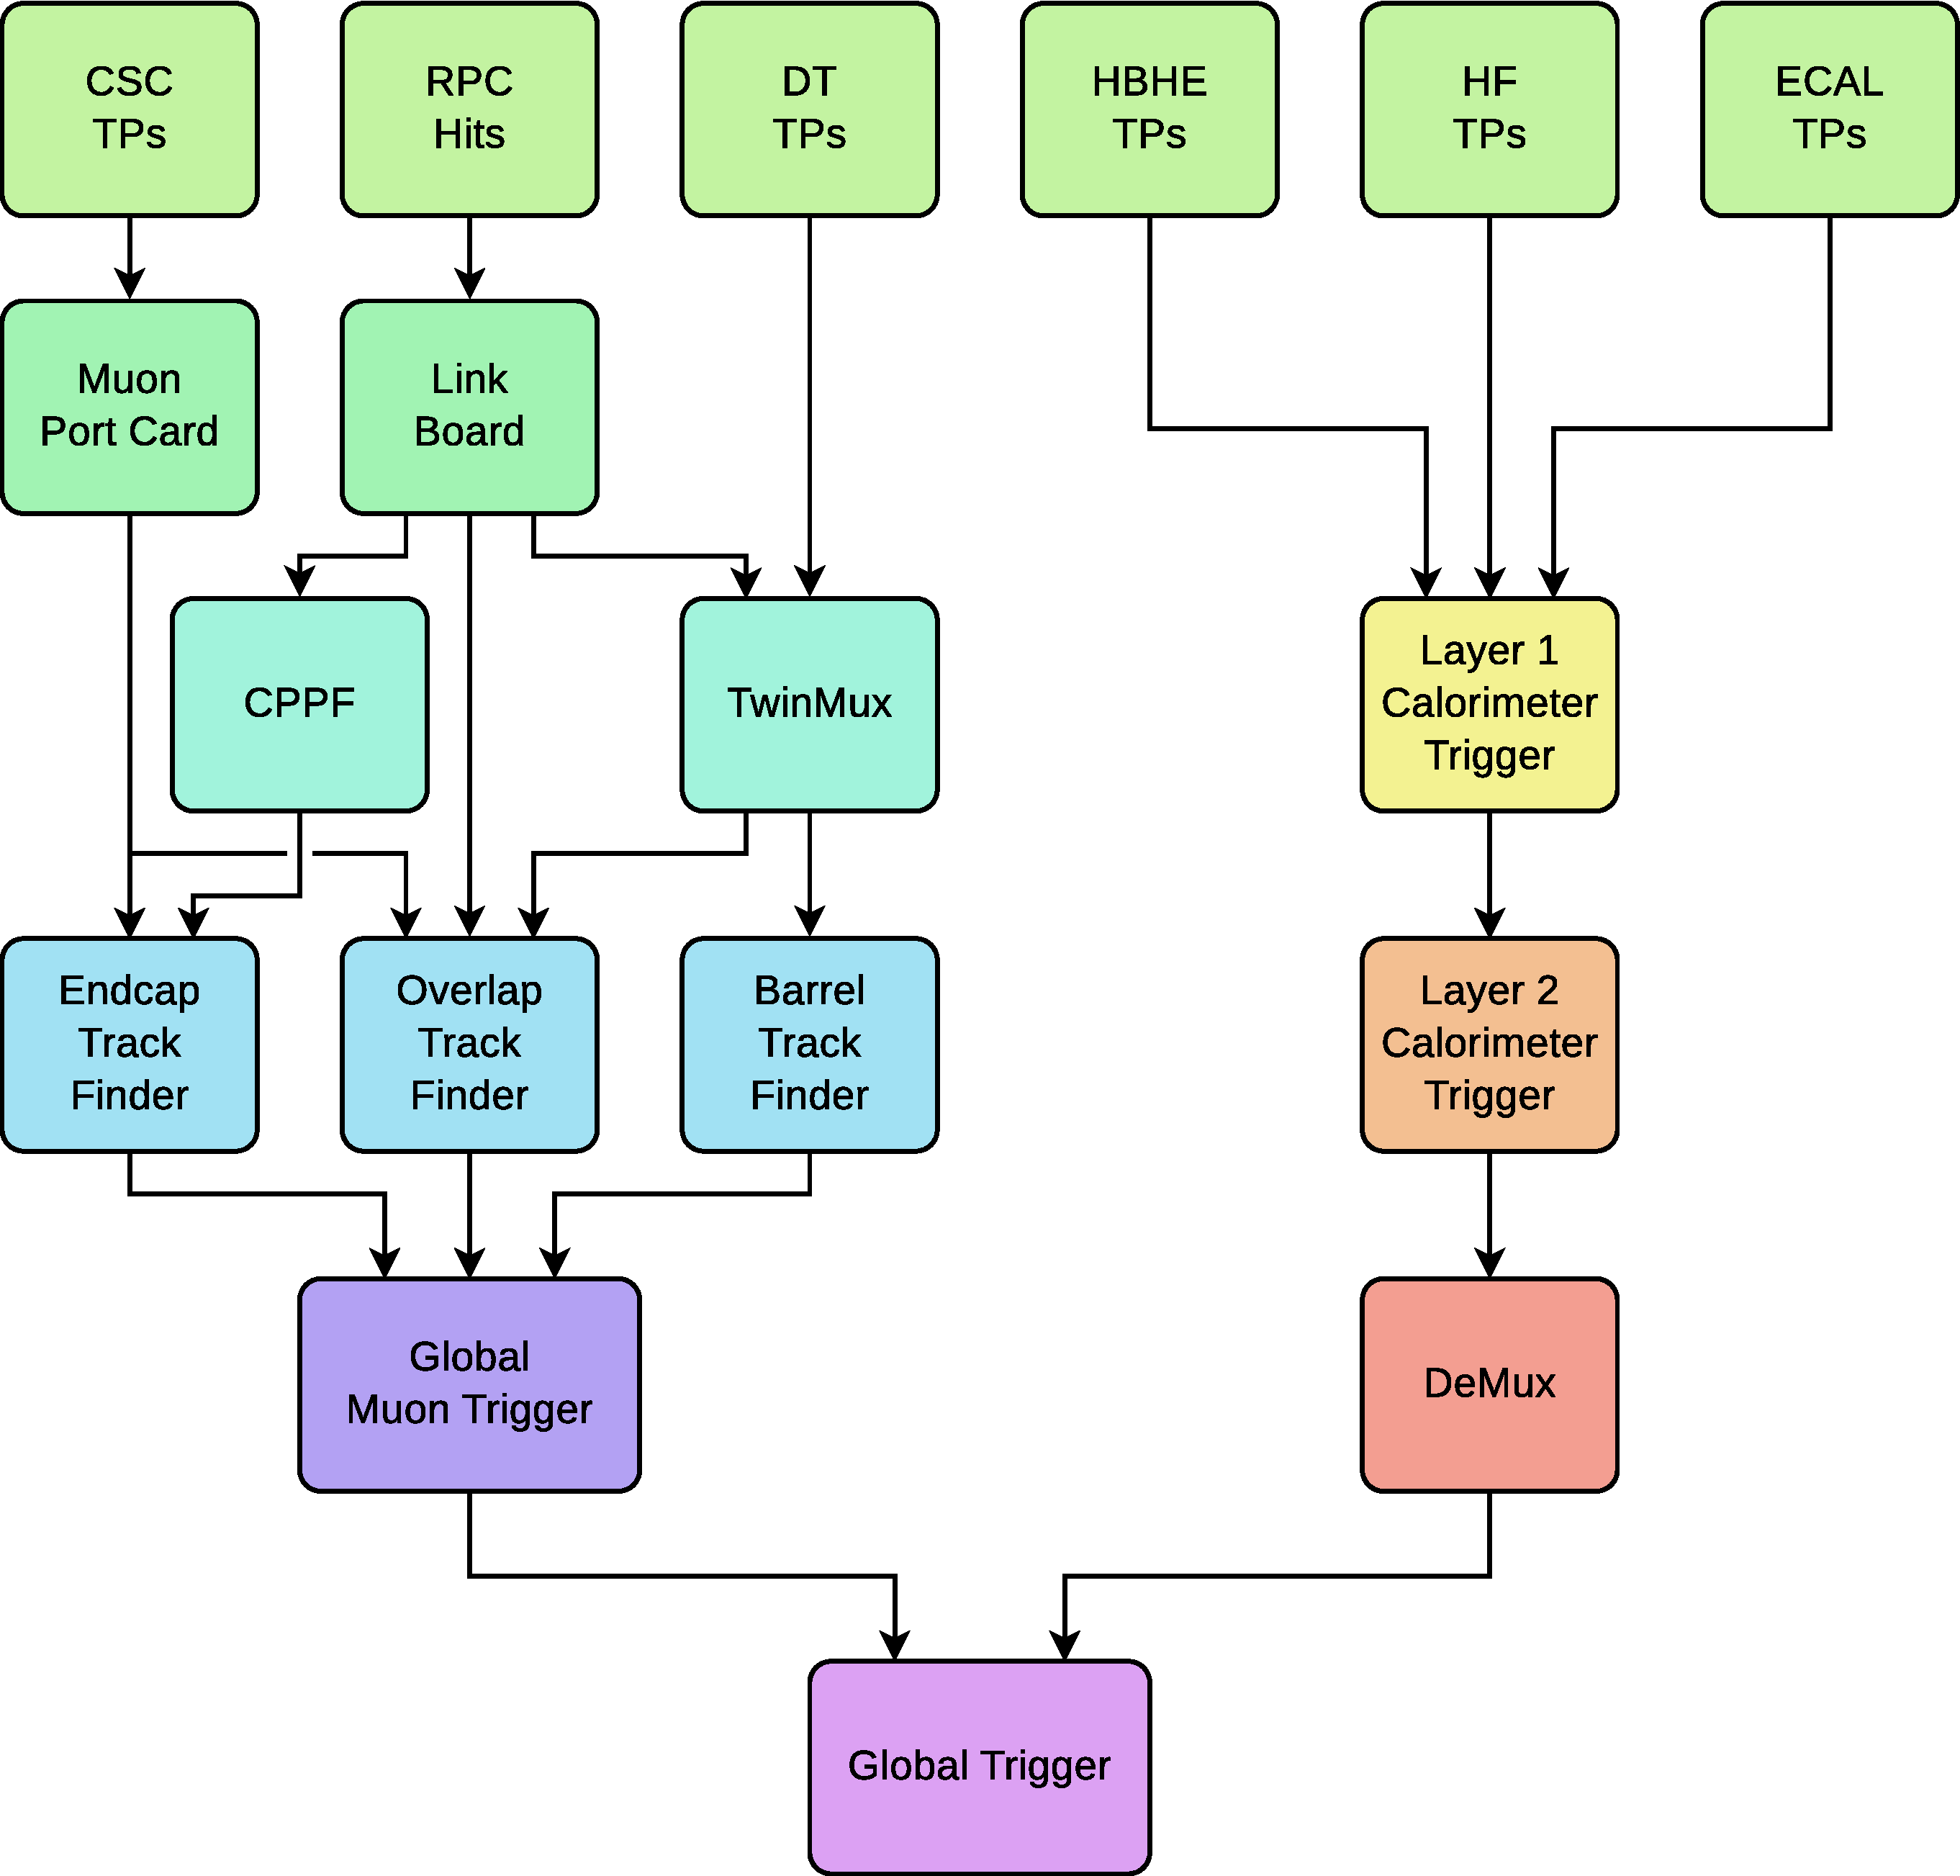
\includegraphics[width=0.65\textwidth]{fig/experiment/cms_L1trigger.pdf}
  \caption{
    Illustration of the L1 Trigger architecture as configured during Run 2.
    The Trigger Primitives (TPs) are generated by track segments or hit patterns in muon chambers, and energy deposits in calorimeters.
    These objects are ranked and sorted by energy, momenta, and quality, which are then passed onto the Global Trigger to determine whether or not the events will be kept and passed to the HLT.
  }
  \label{fig:L1Trigger}
\end{figure}

\subsubsection{High Level Trigger}

% High level trigger
After receiving the L1A signal, the complete readout data from the rest of the detector is sent to the HLT to be further analyzed.
The HLT uses various algorithms to reconstruct the full event and performs tasks such as matching tracks from the inner tracker to muon detection hits in the chambers, or identifying high-energy photons.
Since the HLT is software-based, the algorithms used to reconstruct the events have changed over the operational history of the CMS detector~\cite{Trocino_2014}.
After passing through the HLT, the events are then recorded for offline analysis, and the rate of recorded events after passing through the trigger system as a whole is cut down to be on the order of only a few $10^2\unit{Hz}$.
The recorded events are then passed onto the Data Acquisition (DAQ) system~\cite{Cittolin:578006}.

\subsection{Event Reconstruction}

% Overview
Once the data for an event is processed through the HLT, the event reconstruction process uses the raw detector data to identify particles and jets.
Event reconstruction at CMS is handled through the Particle-Flow (PF) algorithm~\cite{CMS-PAS-PFT-09-001,CMS-PAS-PFT-10-001}, which uses a combination of information from each sub-detector system to identify candidate particles.
In particular, the principal objects identified are electrons, muons, photons, charged hadrons, and neutral hadrons, along with their directions, energies, and types.
These objects can then be used to reconstruct jets to determine quark and gluon energies, determine missing transverse energy \Etmiss resulting from neutrinos and other undetectable particles, reconstruct tau leptons from their decay products, and tag $b$-jets.

% Challenges and demands
Accurately reconstructing the constituents of an event is a challenging task due to the fact that most stable particles that are produced in collisions tend to have low \pt.
For example, in a quark or gluon jet with a \pt of $500\unit{GeV}$, the average \pt carried by its stable constituent particles is on the order of $10\unit{GeV}$, and for jets with a total \pt below $100\unit{GeV}$ this reduces to only a few GeV per stable constituent.
In order to discriminate between jets that produced by heavy exotic particles and those that originate from SM background processes, it is crucial to accurately reconstruct as many final stable particles in the event as possible, many of which will have low \pt and energy.

\subsubsection{The Particle-Flow Algorithm}

% Particle flow overview
The basic elements of PF inputs are objects that come from the CMS sub-detectors: charged particle tracks from the inner tracker, calorimeter clusters, and muon tracks from the muon chambers.
These inputs can be grouped together into objects known as PF blocks through a link algorithm, which are topologically linked together to identify each particle while also avoiding double counting from different detectors.
A block typically contains only one, two, or three of the aforementioned elements from the CMS sub-detectors.
Once the blocks in the event are identified, the Particle-Flow algorithm receives them as input and begins reconstructing individual particles.

% Algorithm outline
The PF algorithm proceeds in the following steps for each block:
\begin{enumerate}
  \item Create PF muons from inner tracker tracks and muon stubs, then remove the corresponding tracks.
  \item Create PF electrons from tracks and ECAL PF clusters if they pass identification criteria, then remove the corresponding tracks.
  \item Tighter quality criteria on the transverse momenta are applied to the remaining tracks to remove fake tracks.
  \item Energies of the remaining ECAL and HCAL PF clusters are calibrated and have the expected energies of the muons from the corresponding clusters subtracted.
  \item Links between ECAL/HCAL clusters and tracks are sorted and either kept or discarded in order to determine which clusters resulted from which tracks.
  \item If the total calibrated calorimetric energy is smaller than the total track momentum by more than three standard deviations, a search for muons and fake tracks is performed with looser criteria.
  \item The remaining tracks result in PF charged hadrons, with the momentum taken from the track momentum if it is not consistent with the calorimetric energy, or obtained from a fit of the measurements in the tracker and the calorimeters.
  \item Neutral particles are identified if the total calibrated cluster energy is larger than the total associated track momentum, with PF photons being created if the calorimetric energy excess is larger than the total ECAL energy, and PF neutral hadrons being created with the remaining part of the excess calibrated ECAL and HCAL energies.
  \item The remaining ECAL and HCAL clusters without links to tracks produce PF photons and PF neutral hadrons, respectively.
\end{enumerate}
After the PF candidates are obtained, they are then used for various tasks in analyses, such as reconstructing jets and determining \Etmiss for the event.

% !TEX root = ../thesis.tex

\chapter{Search for a Heavy Diboson Resonance Produced via Vector Boson Fusion}
\label{chap:analysis}

\section{Introduction}

% Motivation of analysis from theory chapter
In chapter~\ref{chap:theory}, we explored some of the motivation behind BSM searches and examples of BSM theories that predict exotic new particles that may be found in collision events at accelerator facilities.
We also enumerated some of the benchmark models from BSM theories, which were the spin-0 Kaluza-Klein Radion, spin-1 \Wpr/\Zpr boson, and spin-2 Bulk Graviton.
Additionally, we discussed the \VBF production mode that this work focuses on, and the final state that is produced.

% Previous searches
Previous searches have been conducted for dibosonic resonances at both CMS and ATLAS, although none have found evidence of such a resonance being observed at the LHC~\cite{Sirunyan_18,Aaboud_18,Aaboud_18_2,Aad_15,Khachatryan_14,Sirunyan_17,Sirunyan_17_2,atlas20}.
Some of these searches also considered different production modes, as well as other intermediate and final states, such as a \ZZ/\ZH resonance with fully leptonic or hadronic final states.
As mentioned in section~\ref{sec:VBF}, this analysis is itself a continuation of a previous search by the CMS collaboration for a dibosonic resonance using data from 2016.

% VBF analysis as part of the main analysis
While this work focuses on the \VBF production mode, it is one of three modes considered for the full diboson analysis using the Run 2 data.
The other two modes considered involve gluon-gluon fusion (\ggF) and Drell-Yan (\DY) processes.
These additional modes produce identical \lnuqqbarprp and \lnubbbar semileptonic final states, but without the \VBF jets in the forward regions of the detector.
For completeness, we include the full diboson analysis with the non-\VBF production categories in this chapter.
Figure~\ref{fig:nonVbf} shows some example Feynman diagrams of other processes that were considered for the full analysis.

\begin{figure}[htbp]
  \centering
  % !TEX root = ../../thesis.tex
\begin{tikzpicture}
  \begin{feynman}
    % Vertices
    \coordinate (g1) at (135:2.25);
    \coordinate (g2) at (225:2.25);
    \coordinate (x1) at (0,0);
    \coordinate (x2) at (1.5,0);
    \coordinate (v1) at ($(x2)+(45:1.5)$);
    \coordinate (v2) at ($(x2)+(-45:1.5)$);
    \coordinate (q1) at ($(v1)+(25:1.5)$);
    \coordinate (q2) at ($(v1)+(-25:1.5)$);
    \coordinate (l1) at ($(v2)+(25:1.5)$);
    \coordinate (l2) at ($(v2)+(-25:1.5)$);

    \coordinate (q3) at ($(g1)+(8,0)$);
    \coordinate (q4) at ($(g2)+(8,0)$);
    \coordinate (x3) at ($(x1)+(8,0)$);
    \coordinate (x4) at ($(x2)+(8,0)$);
    \coordinate (v3) at ($(v1)+(8,0)$);
    \coordinate (v4) at ($(v2)+(8,0)$);
    \coordinate (q5) at ($(q1)+(8,0)$);
    \coordinate (q6) at ($(q2)+(8,0)$);
    \coordinate (l3) at ($(l1)+(8,0)$);
    \coordinate (l4) at ($(l2)+(8,0)$);

    % Lines
    \draw[gluon] (x1) -- (g1);
    \draw[gluon] (x1) -- (g2);
    \draw[boson] (x1) -- (x2) node[pos=0.5,above] {$X$};
    \draw[boson] (x2) -- (v1) node[pos=0.75,xshift=-0.5cm] {$W$};
    \draw[boson] (x2) -- (v2) node[pos=0.75,xshift=-0.5cm] {$W$};
    \draw[fermion] (v1) -- (q1);
    \draw[fermion] (q2) -- (v1);
    \draw[fermion] (v2) -- (l1);
    \draw[fermion] (l2) -- (v2);

    \draw[fermion] (q3) -- (x3);
    \draw[fermion] (x3) -- (q4);
    \draw[boson] (x3) -- (x4) node[pos=0.5,above] {$X$};
    \draw[scalar] (x4) -- (v3) node[pos=0.75,xshift=-0.5cm] {$H$};
    \draw[boson] (x4) -- (v4) node[pos=0.75,xshift=-0.5cm] {$W$};
    \draw[fermion] (v3) -- (q5);
    \draw[fermion] (q6) -- (v3);
    \draw[fermion] (v4) -- (l3);
    \draw[fermion] (l4) -- (v4);

    % Blobs
    \fill[white] (x1) circle (0.2);
    \fill[white] (x2) circle (0.2);
    \draw[pattern=north west lines] (x1) circle (0.2);
    \draw[pattern=north west lines] (x2) circle (0.2);

    \fill[white] (x3) circle (0.2);
    \fill[white] (x4) circle (0.2);
    \draw[pattern=north west lines] (x3) circle (0.2);
    \draw[pattern=north west lines] (x4) circle (0.2);

    % Label
    \node[anchor=mid,left] at (g1) {$g$};
    \node[anchor=mid,left] at (g2) {$g$};
    \node[anchor=mid,right] at (q1) {$q$};
    \node[anchor=mid,right] at (q2) {$\bar{q}'$};
    \node[anchor=mid,right] at (l1) {$\ell$};
    \node[anchor=mid,right] at (l2) {$\bar{\nu}$};

    \node[anchor=mid,left] at (q3) {$q$};
    \node[anchor=mid,left] at (q4) {$\bar{q}'$};
    \node[anchor=mid,right] at (q5) {$b$};
    \node[anchor=mid,right] at (q6) {$\bar{b}$};
    \node[anchor=mid,right] at (l3) {$\ell$};
    \node[anchor=mid,right] at (l4) {$\bar{\nu}$};
  \end{feynman}
\end{tikzpicture}

  \caption{
    Examples of additional production processes considered in the full analysis that includes non-\VBF production modes.
    We also consider a gluon-gluon fusion process such as a neutral spin-2 resonance decaying to \WW (left), and a Drell-yan process such as a charged spin-1 resonance decaying to \WH (right).
  }
  \label{fig:nonVbf}
\end{figure}

% Details of reconstructing events
In subsection~\ref{subsec:expEvent} we discussed the expected event structure for the decay events of interest, in which the leptonic decay of the $W$ boson results in an $e\nu$ or $\mu\nu$ pair with large missing transverse energy from the neutrino, the hadronic decay of the \VorH boson results in a large single jet with substructure, and \VBF processes produce forward-facing jets.
The boosted topology is a result of the fact that the resonances considered have masses in the TeV range, which causes the $W$ and \VorH bosons to have transverse momenta on the order of several hundred GeV.
This requires the use of specialized techniques to identify and reconstruct the individual $W$ and \VorH bosons based on information from the reconstructed lepton, missing transverse energy of the neutrino, and two-pronged substructure of the jet.
Additionally, the signal models used for the analysis assume that the resonance width is narrow, meaning that the decay width of the resonance in the \WV/\WH diboson mass spectrum is smaller than the experimental resolution.

% Details on modeling background
A unique aspect of the previous analysis that this work inherits is a novel signal extraction method, in which the SM background contribution is estimated from the data using a two-dimensional (2D) maximum likelihood fit.
This process is performed in the plane formed by the mass of the jet from the \VorH decay \MJ, and the invariant mass of the \WV/\WH diboson system \MVV.
Two classes of SM background events are considered for this analysis.
The first is a \WVt background that is resonant in the \MJ spectrum, and the second is a \Wjets contribution that is non-resonant in \MJ.
One advantage of using a 2D fit is the ability to retain more events for modeling background in the sideband regions within the 2D \MJ-\MVV plane, as opposed to looking at the sidebands in the \MJ and \MVV spectra separately.
This also allows for conducting a simultaneous search of \WW, \WZ, and \WH resonances as opposed to performing separate analyses in pre-defined \MJ windows.

% Chapter overview
For this chapter, we examine the complete analysis process of the search for a dibosonic resonance produced in proton-proton collisions at the LHC with center-of-mass energies of $\sqrt{s}=13\unit{TeV}$.
The data used in this analysis were collected over 2016, 2017, and 2018 with integrated luminosities of $35.9\unit{fb^{-1}}$, $41.5\unit{fb^{-1}}$, and $59.7\unit{fb^{-1}}$, respectively.
Section~\ref{sec:samples} provides an overview of the data and simulation samples that were used for the analysis.
In section~\ref{sec:events}, we discuss the selection cuts used to determine which events are used from the data and simulation samples.
We then go over the SM sources of background and how they are taken into account for the analysis in section~\ref{sec:bkg}, followed by the signal modeling process in section~\ref{sec:sig}.
The fit validation and bias testing procedures are described in section~\ref{sec:bias}, after which we discuss the results of the search in section~\ref{sec:results}.

\section{Data and Simulation Samples}
\label{sec:samples}

% The need for simulation samples of signal and background
This search uses the proton-proton collision data collected by the CMS detector during Run 2.
The data are collected and stored for analysis after events generate trigger primitives in the detector subsystems and get passed through the HLT as described in chapter~\ref{chap:exp}.
We also list the Monte Carlo (MC) signal samples used in the analysis that are based on the BSM models of subsection~\ref{subsec:benchmark}.
Additionally, we list the MC samples that model SM background contributions to the search.
Complete lists of each sample used are found in appendix~\ref{chap:appendixSamples}.

% Data samples
The data are listed in tables~\ref{tab:dataSamples2016}-\ref{tab:dataSamples2018}, along with their integrated luminosities.
For each year of Run 2, documentation is available for the luminosity measurements~\cite{CMS-PAS-LUM-17-001,CMS-PAS-LUM-17-004,CMS-PAS-LUM-18-002}.
The data are divided into three sets per year, with contributions from the \texttt{SingleMuon}, \texttt{SingleElectron}, and \texttt{MET} sets.

% Signal samples
This analysis makes use of ten benchmark signal models, which are listed in tables~\ref{tab:ggFGBulkToWWSamples}-\ref{tab:VBFZprToWWSamples} with their cross sections and branching ratios.
The signal models used are \ggF/\VBF\GBulktoWWtolnuqqbarpr, \ggF/\VBF\RadtoWWtolnuqqbarpr, \DY/\VBF\WprtoWZtolnuqqbar, \DY/\VBF\WprtoWHtolnubbbar, and \DY/\VBF\ZprtoWWtolnuqqbarpr.
Each signal has different samples for each year of Run 2, for a total of three sets of samples per signal.
Furthermore, each signal has separate samples with 50,000 events for the following resonance masses: 0.8, 1, 1.2, 1.4, 1.6, 1.8, 2.0, 2.5, 3.0, 3.5, 4.0, and $4.5\unit{TeV}$\footnote{The 2016 \VBF\ZprtoWW and 2016 \VBF\WprtoWZ sets are the exception to this, lacking mass values below $1.2\unit{TeV}$.}.
Additional details on the parameters for each model are discussed in section~\ref{sec:sigSamples} of appendix~\ref{chap:appendixSamples}.

% Background samples
Finally, MC samples are also used to simulate SM background contributions, as listed in tables~\ref{tab:bkg2016Samples} and \ref{tab:bkg2017Samples} along with their cross sections.
These background samples include various processes that are broadly categorized as \Wjets and \WVt, some of which include DY+jets, QCD, and $t\bar{t}$ production samples.
% More on background samples

\section{Event Selection and Categorization}
\label{sec:events}

% Goal of event selection
In subsection~\ref{subsec:expEvent}, we described the expected event topology for the \WV/\WH dibosonic resonance that this work searches for.
In particular, the semileptonic decay produces a highly energetic lepton ($e$ or $\mu$) and large \Etmiss from the neutrino from the \Wtolnu decay, a large-radius jet from the hadronic \Vtoqqbarpr or \Htobbbar decay, and forward-facing \VBF jets for \VBF-produced resonances.
To select for possible events that exhibit the expected final state structure, selection cuts must be made that capture the expected behavior and reduce background.
This section provides an overview of the cuts that were made in the analysis to optimize the search for the \WV/\WH dibosonic resonance.

\subsection{Trigger}

% Trigger paths
There are multiple HLT trigger paths that used for recording the data that this analysis uses.
Most of the data are collected from the single electron and single muon triggers, with the remainder coming from the single photon, EGamma, and MET triggers.
For each year we use different paths, which are listed in tables~\ref{tab:triggers2016}, \ref{tab:triggers2017}, and \ref{tab:triggers2018} for the years 2016, 2017, and 2018, respectively.

\begin{table}[htbp]
  \centering
  % !TEX root = ../../thesis.tex
\footnotesize
\begin{tabular}{l|l|c}
  \hline
  Dataset        & HLT paths                                    & Description\\
  \hline \hline
  \ttfamily SingleElectron/& \ttfamily HLT\_Ele27\_WPTight\_Gsf\_v*                 & $\pt>27\unit{GeV}$, Tight WP for ele ID  \\
  \ttfamily SinglePhoton   & \ttfamily OR HLT\_Ele45\_WPLoose\_Gsf\_v*              & $\pt>45\unit{GeV}$, Loose WP for ele ID  \\
                 & \ttfamily OR HLT\_Ele115\_CaloIdVT\_GsfTrkIdT\_v*      & $\pt>115\unit{GeV}$  \\
                 & \ttfamily OR HLT\_Photon175\_v*                        & $\Et>175\unit{GeV}$  \\
  \hline
  \ttfamily SingleMuon     & \ttfamily HLT\_Mu50\_v*                                & $\pt>50\unit{GeV}$ \\
                 & \ttfamily OR HLT\_TkMu50\_v*                           & tracker muon, $\pt>50\unit{GeV}$ \\
  \hline
  \ttfamily MET            & \ttfamily HLT\_PFMETNoMu120\_PFMHTNoMu120\_IDTight\_v* & $\Etmiss>120\unit{GeV}$ \\
  \hline
\end{tabular}

  \caption{
    HLT paths used in 2016 data and MC.
  }
  \label{tab:triggers2016}
\end{table}

\begin{table}[htbp]
  \centering
  % !TEX root = ../../thesis.tex
\footnotesize
\begin{tabular}{l|l|c}
  \hline
  Dataset        & HLT paths                                    & Description\\
  \hline \hline
  \ttfamily SingleElectron/& \ttfamily HLT\_Ele32\_WPTight\_Gsf\_v*                 & $\pt>32\unit{GeV}$, Tight WP for ele ID  \\
  \ttfamily SinglePhoton   & \ttfamily OR HLT\_Ele35\_WPTight\_Gsf\_v*              & $\pt>35\unit{GeV}$, Tight WP for ele ID  \\
                 & \ttfamily OR HLT\_Ele115\_CaloIdVT\_GsfTrkIdT\_v*      & $\pt>115\unit{GeV}$  \\
                 & \ttfamily OR HLT\_Photon200\_v*                        & $\Et>200\unit{GeV}$  \\
  \hline
  \ttfamily SingleMuon     & \ttfamily HLT\_Mu50\_v*                                & $\pt>50\unit{GeV}$ \\
                 & \ttfamily OR HLT\_OldMu100\_v*                         & $\pt>100\unit{GeV}$ \\
                 & \ttfamily OR HLT\_TkMu100\_v*                          & tracker muon, $\pt>100\unit{GeV}$ \\
  \hline
  \ttfamily MET            & \ttfamily HLT\_PFMETNoMu120\_PFMHTNoMu120\_IDTight\_v* & $\Etmiss>120\unit{GeV}$ \\
  \hline
\end{tabular}

  \caption{
    HLT paths used in 2017 data and MC.
  }
  \label{tab:triggers2017}
\end{table}

\begin{table}[htbp]
  \centering
  % !TEX root = ../../thesis.tex
\footnotesize
\begin{tabular}{l|l|c}
  \hline
  Dataset        & HLT paths                                    & Description\\
  \hline \hline
  \ttfamily EGamma         & \ttfamily HLT\_Ele32\_WPTight\_Gsf\_v*                 & $\pt>32\unit{GeV}$, Tight WP for ele ID  \\
                 & \ttfamily OR HLT\_Ele115\_CaloIdVT\_GsfTrkIdT\_v*      & $\pt>115\unit{GeV}$  \\
  \hline
  \ttfamily SingleMuon     & \ttfamily HLT\_Mu50\_v*                                & $\pt>50\unit{GeV}$ \\
                 & \ttfamily OR HLT\_OldMu100\_v*                         & $\pt>100\unit{GeV}$ \\
                 & \ttfamily OR HLT\_TkMu100\_v*                          & tracker muon, $\pt>100\unit{GeV}$ \\
  \hline
  \ttfamily MET            & \ttfamily HLT\_PFMETNoMu120\_PFMHTNoMu120\_IDTight\_v* & $\Etmiss>120\unit{GeV}$ \\
  \hline
\end{tabular}

  \caption{
    HLT paths used in 2018 data and MC.
  }
  \label{tab:triggers2018}
\end{table}

% Single electron thresholds
The single electron \pt thresholds used are 27, 45, and $115\unit{GeV}$ for 2016, 32, 25, and $115\unit{GeV}$ for 2017, and 25 and $115\unit{GeV}$ for 2018. % Check why the threshold is 25 and not 32 for 2018
Additionally, we apply an OR with \texttt{HLT\_Photon175} in 2016 with an \Et threshold of $175\unit{GeV}$, as well as with \texttt{HLT\_Photon200} in 2017 with $200\unit{GeV}$. % Need to find out what an OR is
These thresholds were applied as recommended by the CMS E/Gamma Physics Object Group (POG)~\cite{MuonPOG}.

% Single muon thresholds
For the muon thresholds, the main threshold is $50\unit{GeV}$ across all three years, with an OR for \texttt{HLT\_TkMu50} at $50\unit{GeV}$ in 2016, and an OR for \texttt{HLT\_OldMu100} in 2017 and \texttt{HLT\_TkMU100} in 2018 at $100\unit{GeV}$, as recommended by the Muon POG~\cite{MuonHLT2016,MuonHLT2017,MuonHLT2018}.

% Additional explanation of efficiencies?
% Possibly add subsection on prefiring weights

\subsection{Pileup Reweighting}

The data samples from all three Run 2 years have different pileup (PU) profiles than that of the simulation samples that were used for this analysis.
In order to account for this, we compute and apply PU weights to our samples and compare distributions for the number of primary vertices both with and without weights to the data.
Figure~\ref{fig:PUreweight} shows these distributions for 2016, 2017, and 2018.
The weights are computed using the recommended minimum bias cross section of $69.2\unit{mb}$. % Citation needed

\begin{figure}[htbp]
  \centering
  \includegraphics[width=0.45\textwidth]{fig/analysis/PUrewN_0_2016_nVert.pdf}
  \includegraphics[width=0.45\textwidth]{fig/analysis/PUrewN_0_2017_nVert.pdf}\\
  \includegraphics[width=0.45\textwidth]{fig/analysis/PUrewN_0_2018_nVert.pdf}
  \caption{
    Distribution of the number of primary vertices reconstructed in simulation before and after pileup reweighting, with data present, for 2016 (top left), 2017 (top right), and 2018 (bottom).
  }
  \label{fig:PUreweight}
\end{figure}

\subsection{Muon Selection}
\label{subsec:muonSelect}

% High-pT muon selection criteria
When selecting muons for the analysis, they must pass the following high-\pt muon identification criteria as provided by the CMS Muon POG~\cite{MuonSelection}:
\begin{itemize}
  \item The muon is reconstructed as a ``global'' muon.
  \item At least one muon-chamber hit included in the global-muon track fit or in the TuneP fit.
  \item Muon segments in at least two muon stations.
  \item The \pt relative error ($\sigma(\pt)/\pt$) of the muon best track is less than 30\%.
  \item Its tracker track has transverse impact parameter $d_{xy}<2\unit{mm}$ with respect to the primary vertex.
  \item The longitudinal distance of the tracker with respect to the primary vertex is $d_z<5\unit{mm}$.
  \item The muon track has at least one pixel hit.
  \item The muon track has at least six tracker layer hits.
\end{itemize}

% Further muon selection
In addition to the high-\pt muon identification criteria, for this analysis we also require each muon to have $\pt>55\unit{GeV}$ and to be confined to the region $|\eta|<2.4$.
We also apply an isolation requirement on the muons in order to further suppress background.
This is done using the full relative particle flow isolation using $\Delta\beta$ corrections, with the requirement that $I_\mathrm{rel}<0.05$.

Scale factors for muon ID as provided by the Muon POG are also applied~\cite{MuonPAGs}.
To appropriately apply these scale factors as they vary by year to the full Run 2 data set, we weight them by the fraction of integrated luminosity for each year.
We also apply a scale factor for the isolation requirement, which is shown in figure~\ref{fig:muonIsoSF}.
This scale factor was derived on top of muon high-\pt ID, in boosted $Z$ and DY events over the full Run 2 period, which is found to be within 1\% from unity and smaller than the systematic uncertainty for the muon trigger/reco/ID of 5\% used in signal extraction.

\begin{figure}[htbp]
  \centering
  \includegraphics[width=0.65\textwidth]{fig/analysis/muonFullIsoSF.pdf}
  \caption{
    Efficiency in data and simulation and data/MC scale factor for muon isolation requirement.
  }
  \label{fig:muonIsoSF}
\end{figure}

\subsection{Electron Selection}
\label{subsec:elecSelect}

% Electron reconstruction
The electrons that are reconstructed from trigger primitives in the ECAL are required to pass the ``HEEP v7.0'' ID requirements as prescribed by the E/Gamma POG~\cite{HEEPV70}.
The ID requirements ensure that the reconstructed electrons from the ECAL energy deposits are paired with a high quality track from the inner tracker and have a shape consistent with an electromagnetic shower in the calorimeter.
These requirements are listed in table~\ref{tab:HEEPV70}.
For our analysis, we also require them to have $\pt>55\unit{GeV}$ and be within the pseudorapidity range $|\eta|<2.5$, except for the region $[1.4442,1.566]$. % Unsure why this range is excluded
We also apply scale factors for the HEEP ID requirements along with RECO scale factors as recommended by the E/Gamma POG~\cite{EgammaScale}.

\begin{table}[htbp]
  \centering
  % !TEX root = ../../thesis.tex
\footnotesize
\begin{tabular}{lll}
  \hline
  Variable                          & Barrel                             & Endcap                             \\
  \hline
  \multicolumn{3}{c}{Acceptance selections}\\
  \Et                               & $\Et>35\unit{GeV}$                 & $\Et>35\unit{GeV}$                 \\
  $\eta$                            & $|\eta_{SC}|<1.4442$               & $1.566<|\eta_{SC}|<2.5$            \\
  \multicolumn{3}{c}{Identification selections}\\
  \texttt{isEcalDriven}             & \texttt{true}                      & \texttt{true}                      \\
  $\Delta\eta_\mathrm{in}^\mathrm{seed}$          & $|\Delta\eta_\mathrm{in}^\mathrm{seed}|<0.004$ & $|\Delta\eta_\mathrm{in}^\mathrm{seed}|<0.006$ \\
  $\Delta\phi_\mathrm{in}$                 & $|\Delta\phi_\mathrm{in}|<0.06$         & $|\Delta\phi_\mathrm{in}|<0.06$         \\
  $H/E$                             & $H/E<1/E+0.05$                 & $H/E<5/E+0.05$                 \\
  $\sigma_{i\eta i\eta}$            & -                                  & $\sigma_{i\eta i\eta}<0.03$      \\
  $\frac{E_{1\times5}}{E_{5\times5}}$, $\frac{E_{2\times5}}{E_{5\times5}}$        & $\frac{E_{1\times5}}{E_{5\times5}}>0.83$ or $\frac{E_{2\times5}}{E_{5\times5}}>0.94$ & -                              \\
  Inner lost layer hits             & lost hits $\leq1$                  & lost hits $\leq1$                  \\
  Impact parameter, $d_{xy}$        & $|d_{xy}|<0.02$                    & $|d_{xy}|<0.05$                    \\
  \multicolumn{3}{c}{Isolation selections}\\
  EM + had depth 1                  & $iso<2+0.03\Et+0.28\rho$     & $iso<2.5+0.28\rho$ ($\Et<50\unit{GeV}$) \\
  isolation, $iso$                  &                                    & else $iso<2.5+0.03(\Et-50\unit{GeV})+0.28\rho$ \\
  $\pt$ isolation, $isopt$          & $isopt<5\unit{GeV}$                   & $isopt<5\unit{GeV}$                   \\
  \hline
\end{tabular}

  \caption{
    Definitions of HEEP ID V7.0 selections.
  }
  \label{tab:HEEPV70}
\end{table}

\subsection{Jet Selection}
\label{subsec:jetSelect}

% Types of jets
As mentioned previously, there are two types of jets that are expected to be produced in the signal events of interest.
The first is a large-radius jet that is produced via the \VorH decay that exhibits two-pronged substructure, while the second type are small-radius forward-facing jets only present in \VBF production modes.
This analysis therefore categorizes candidate jets into the two following types:
\begin{itemize}
  \item ``Large-radius'' AK8 jets: \VorH boson candidates that decay into $q\bar{q}^{(\prime)}$ or $b\bar{b}$, using the anti-$k_\mathrm{T}$ algorithm with distance parameter $R=0.8$.
  \item ``Standard'' AK4 jets: \VBF forward jet candidates, using the anti-$k_\mathrm{T}$ algorithm with distance parameter $R=0.4$.
\end{itemize}

% The anti-kt algorithm
The anti-$k_\mathrm{T}$ algorithm is a jet clustering algorithm reconstructs jets by introducing distances $d_{ij}$ between objects $i$ and $j$ and $d_{i,B}$ between object $i$ and the beam $B$~\cite{Cacciari_2008}.
The algorithm starts by assigning values for $d_{ij}$ and $d_{i,B}$ for all objects in the final state, and finds the minimum value among the distances.
If the minimum value is a $d_{i,B}$ value, then object $i$ is declared to be a jet and removed from the list, and the algorithm starts over from the first step.
If instead it is a $d_{ij}$ value, then objects $i$ and $j$ are combined and the algorithm goes back to the first step.
This process is repeated until all particles have been declared jets, with $d_{ij}$ and $d_{i,B}$ defined by
\begin{align}
  d_{ij} &= \min\pqty{k_{\mathrm{T},i}^{2p},k_{\mathrm{T},j}^{2p}}\frac{\Delta_{ij}^2}{R^2},\\
  d_{i,B} &= k_{\mathrm{T},i}^{2p},
\end{align}
where $\Delta_{ij}^2=(y_i-y_j)^2+(\phi_i-\phi_j)^2$, with $k_{T,i}$ as the transverse momentum for object $i$, $y_i$ the rapidity for object $i$, $\phi_i$ is the azimuthual angle for object $i$, $R$ is the distance parameter for the algorithm, and $p$ is a parameter determined by the jet clustering algorithm.
For the anti-$k_\mathrm{T}$ algorithm, $p=-1$, with other algorithms taking on different values, such as $p=1$ for the $k_\mathrm{T}$ algorithm~\cite{shelton2013tasi}.

% Jet selection
For both types of jets, we use tight ID jets as recommended by the JetMET POG~\cite{jetID2016,jetID2017,jetID2018}.
We also apply jet energy corrections for data and MC prescribed by the Jet Energy Resolution and Corrections (JERC) subgroup~\cite{JetEnergyScale}.
The hadronic jet resulting from the \VorH decay is selected by taking the jet with the highest \pt from the large-radius jets, with a minimum threshold of $\pt>200\unit{GeV}$ and a pseudorapidity range of $|\eta|<2.4$.
Any large-radius jets that have an electron or tight muon within $\Delta R=\sqrt{\Delta\eta^2+\Delta\phi^2}<1.0$ are discarded to suppress background events.
For the standard jets, we require that $\pt>30\unit{GeV}$, and we discard any jets within $\Delta R<0.4$ of any tight electron or tight muon, or within $\Delta R<0.8$ of any large-radius jet.

\subsubsection{$V$-jet Tagging}

% V-jet identification
A central component of the analysis is the ability to accurately identify and reconstruct the hadronically decaying \VorH boson, which we shall refer to as \Vhad.
Once the jets in the final state are identified, algorithms must be applied to determine the substructure of the jets.
This analysis makes use of the Pileup Per Particle Identification (PUPPI) algorithm, which takes particle flow object candidates and assigns weights to each particle based energy shape profiles~\cite{Bertolini_2014}.
The resulting reweighted candidates are then put into substructure algorithms for further analysis.

% Jet grooming
The jets obtained from the PUPPI algorithm are then groomed by using the ``soft drop'' algorithm~\cite{Larkoski_2014}, which removes soft wide-angle radiation from jets.
For a jet with radius $R$ with two constituents, the soft drop algorithm removes the softer constituent if it does not satisfy the condition
\begin{equation}
  \frac{\min\pqty{p_{\mathrm{T},1},p_{\mathrm{T},2}}}{p_{\mathrm{T},1}+p_{\mathrm{T},2}}>z\pqty{\frac{\Delta R_{12}}{R}}^\beta,
\end{equation}
where the $p_{\mathrm{T},i}$ are the transverse momenta of the jet constituents, $\Delta R_{12}$ is the separation between the constituents in the $y$-$\phi$ plane, $R$ is the radius of the jet, $z$ is the soft drop threshold, and $\beta$ is the angular exponent.
For this analysis, we use $z=0.1$ based on theoretical considerations of the jet mass from QCD~\cite{Dasgupta_2013,Dasgupta_2013_2}.
We denote the soft-drop mass by \MJ, and apply corrections as recommended by JetMET POG~\cite{WZ-tagging}.

% N-subjettiness
To determine the degree to which the jet has substructure, we use the ``$N$-subjettiness'' as a measure of how many subjets are present in the jet~\cite{Thaler_2011,Thaler_2012}.
It is designed to identify boosted hadronic objects based on the angular distances of jet constituents relative to their nearest subjet axis.
Figure~\ref{fig:jetSubstruct} shows an example of a jet with two subjects defined by axes $\mathbf{\hat{n}}_1$ and $\mathbf{\hat{n}}_2$, which is the two-pronged structure expected to be observed by the \Vhad boson decay.
We proceed by reclustering the jets with the $k_\mathrm{T}$ algorithm until $N$ jets remain, then compute the $N$-subjettiness defined by
\begin{equation}
  \tau_N=\frac{1}{d_0}\sum_kp_{\mathrm{T},k}\min\pqty{\Delta R_{1,k},\Delta R_{2,k},\ldots,\Delta R_{N,k}},
\end{equation}
where $d_0$ is a normalization factor given by
\begin{equation}
  d_0=\sum_kp_{\mathrm{T},k}R_0,
\end{equation}
with $R_0$ as the clustering parameter of the original jet, $p_{\mathrm{T},k}$ is the transverse momentum of the $k$-th jet constituent, and $\Delta R_{n,k}$ is the distance to the $n$-th subject in the $\eta$-$\phi$ plane.

\begin{figure}[htbp]
  \centering
  % !TEX root = ../../thesis.tex
\begin{tikzpicture}
  % Main jet
  \draw[rotate around={270:(0,0)},dotted,thick] (0,7) ellipse (2.6 and 1.3);
  \draw[rotate around={270:(0,0)},dotted,thick] (0,0) -- (69.29:7.21);
  \draw[rotate around={270:(0,0)},dotted,thick] (0,0) -- (110.71:7.21);

  % Subjets
  \draw[rotate around={270:(0,0)},dotted,thick] (1.25,7) ellipse (0.975 and 0.4875);
  \draw[rotate around={270:(0,0)},dotted,thick] (0,0) -- (72.275:7.26);
  \draw[rotate around={270:(0,0)},dotted,thick] (0,0) -- (87.75:7.01);
  \draw[rotate around={270:(0,0)},dotted,thick] (-1.25,7) ellipse (0.975 and 0.4875);
  \draw[rotate around={270:(0,0)},dotted,thick] (0,0) -- (92.25:7.01);
  \draw[rotate around={270:(0,0)},dotted,thick] (0,0) -- (107.725:7.26);

  % Axes
  \draw[->,thick] (0,0) -- (10.12:8.5) node[right] {$\mathbf{\hat{n}}_1$};
  \draw[->,thick] (0,0) -- (-10.12:8.5) node[right] {$\mathbf{\hat{n}}_2$};
\end{tikzpicture}

  \caption{
    Illustration of jet substructure for a two-pronged jet with axes $\mathbf{\hat{n}}_1$ and $\mathbf{\hat{n}}_2$.
    The $N$-subjettiness $\tau_N$ is used as a measure of how many subjets are present within a jet.
  }
  \label{fig:jetSubstruct}
\end{figure}

% N-subjettiness ratios
In some cases it is advantageous to consider ratios of $N$-subjettiness.
For example, in this analysis we consider the ratio $\tau_2/\tau_1=\nsubj$, which is a measure of whether or not the jet exhibits the properties we would expect from a jet with 2 subjets versus a single jet with no substructure.
This allows for separating jets originating from boosted vector bosons versus jets that are produced from quarks and gluons, thereby allowing further background suppression.
This analysis uses a modified version of the $N$-subjettiness ratio that reduces the dependency of \nsubj on the jet mass, which is denoted by the designed decorrelated tagger (DDT) $N$-subjettiness \nsubjDDT~\cite{Dolen_2016}.
It is defined by
\begin{equation}
  \nsubjDDT=\nsubj-C\ln\pqty{\frac{\MJ^2}{\ptjet\times(1\unit{GeV})}},
\end{equation}
where $C$ is a coefficient obtained by taking the slope of a fit for the \nsubj profile versus $\ln\pqty{\frac{\MJ^2}{\ptjet\times(1\unit{GeV})}}$ in non-resonant \Wjets background events after applying the full analysis selection cuts.

% N-subjettiness selection
For this analysis, we only consider large-radius jets that satisfy $\nsubjDDT<0.80$.
We also later use \nsubjDDT for event categorization to split the analysis into high and low purity jet categories.

\subsubsection{$b$-tagging}

% CHS approach
While the boosted jets resulting from the \Vhad decay are identified and groomed using algorithms such as the anti-$k_\mathrm{T}$ and PUPPI algorithms, the candidate four vector for the $X$ boson is estimated using jet energy scale corrections and charged hadron subtraction (CHS).
The CHS approach is used in order to suppress background contribution from top quark production, which results in the production of jets from $b$ decays.

% b-tagging details
Jets in the region $|\eta|<2.4$ are $b$-tagged if they pass the \texttt{medium} working point of the Combined Secondary Vertex (CSV) or DeepCSV algorithms, as recommended by the $b$-tag and vertexing (BTV) POG.
The \texttt{medium} working point for CSV is 0.8484 in 2016~\cite{bTagging2016}, and for DeepCSV the working points are 0.4941 and 0.4184 for 2017 and 2018, respectively~\cite{bTagging2017,bTagging2018}.
We also apply $b$-tagging scale factors and weights that depend on the jet \pt, $\eta$, and value of the $b$-tagging discriminant as prescribed by the BTV POG~\cite{bTaggingEff,bTaggingSF}.

\subsubsection{$H(b\bar{b})$-tagging}

% The need for bb-tagging
The $V$-tagging methods previously described account for identifying and grooming jets resulting from the $\Vhad$ decay, but additional techniques are applied in this analysis to account for a large-radius \bbbar jet.
Such a jet signifies the decay \Htobbbar in the final state and hence a \WH resonance, which allows for discriminating against background with light jet flavors.
For this reason, we use a $b$-tagging discriminator to identify Higgs boson jet candidates that uses information from displaced tracks and secondary vertices~\cite{CMS-PAS-BTV-15-002}.
We also apply a cut on the M2 operating point of the ``DoubleB tagger'' to categorize events, for which the threshold is 0.8 for 2016, 2017, and 2018 according to references~\cite{bTagging2016,bTagging2017,bTagging2018}.

% Scale factors
Additionally, we apply scale data/MC efficiency scale factors to our signal sample normalizations as recommended by the BTV POG, while the scale factors for the background are estimated from the data in the control regions.
We use two sets of scale factors that depend on \ptjet.
One is for \Htobbbar jets resulting from the \WprtoWHtolnubbbar signal model, and the other is for mistagging $W$ bosons resulting from $t\bar{t}$ events, which are applied to the \GBulktoWWtolnuqqbarpr and \WprtoWZtolnuqqbar signal models.
These scale factors are applied from method 1a from reference~\cite{bTaggingEff}.
First we measure the MC $bb$-tagging efficiencies $\epsilon$, then apply the event weights for the \bbbar-tagged category as
\begin{equation}
  w^{\bbbar}(\pt)=\frac{\mathrm{SF}(\pt)\epsilon(\pt)}{\epsilon(\pt)}=\mathrm{SF}(\pt),
\end{equation}
where $\mathrm{SF}$ denotes the scale factors.
For the \bbbar-untagged category, we instead use
\begin{equation}
  w^{\mathrm{no}\bbbar}(\pt)=\frac{1-\mathrm{SF}(\pt)\epsilon(\pt)}{1-\epsilon(\pt)}.
\end{equation}

\subsection{Missing Transverse Energy}

% MET
For this analysis, we use type-I corrected particle flow MET (PFMET) to account for the energy of the neutrino from the \Wlep decay, where PFMET is defined as the magnitude of the negative vector sum of all transverse energies from particle flow objects~\cite{PFMET}.
The correction is a propagation of the jet energy corrections (JEC) to MET, which is given by
\begin{equation}
  \EtmissTI=\vqty{-\sum_\mathrm{jet}\mathbf{p}_\mathrm{T,jet}^\mathrm{JEC}-\sum_{i\in\mathrm{uncl.}}\mathbf{p}_{\mathrm{T},i}},
\end{equation}
where the first sum is over clustered jets and the second sum is over unclustered particles.

\subsection{Leptonic $W$ and \WV reconstruction}

% Leptonic reconstruction
To reconstruct the leptonically decaying $W$ candidate \Wlep, we select the highest \pt lepton in the event and combine it with the \EtmissTI resulting from the neutrino.
We also apply a $W$ mass constraint to estimate the $z$-component of the missing energy.
The resulting \Wlep is then combined with the large-radius \Vhad jet to form a diboson candidate, with mass denoted by \MVV.

\subsection{VBF Forward Jets}
\label{subsec:VBFjets}

% VBF signature
The defining signature of the \VBF production process is the presence of two boosted jets in the forward and backward regions of the detector, along with the decay products in the central region of the detector resulting from the \Wlep and \Vhad resonances.
The analysis therefore requires additional kinematic constraints in order to categorize \VBF-produced events, which take into account properties of the forward-facing \VBF jets such as their combined mass and separation in $\eta$.

% VBF jet selection
We select candidate \VBF jets from the two highest \pt standard AK4 jets as defined in subsection~\ref{subsec:jetSelect}.
This requires that the \VBF jets pass $\pt>30\unit{GeV}$, and that they do not overlap with the selected lepton and large-radius jet.
We then apply selection cuts to the two candidate \VBF jets based on their separation in pseudorapidity \DetaVBF and \VBF dijet mass \mjjVBF.

% VBF Deta selection cut
For the cut on \DetaVBF, we exploit the fact that the \VBF jets are expected to be found in the high $|\eta|$ regions of the detector near the endcaps and be roughly anti-parallel to each other.
Figure~\ref{fig:detaSB_VBF} (left) shows the relative shape differences in \DetaVBF between the \VBF\RadtoWW signal MC sample and the background MC samples used in this analysis.
To retain a signal efficiency of 40-50\%, we choose a cut of $\DetaVBF>4$.

\begin{figure}[htbp]
  \centering
  \includegraphics[width=0.45\textwidth]{fig/analysis/detaSB.pdf}
  \includegraphics[width=0.45\textwidth]{fig/analysis/mjjSB.pdf}\\
  \caption{
    Shape comparison of a \VBF\RadtoWW signal sample and background MC samples, normalized to unity, for \DetaVBF (left) and \mjjVBF (right).
    The shape discrepancy between the \VBF signal and background distributions in \DetaVBF and \mjjVBF allows for distinguishing signal from background.
  }
  \label{fig:detaSB_VBF}
\end{figure}

% VBF dijet mass selection cut
The other kinematic cut applied to the \VBF candidate jets is on the invariant mass of the sum of the \VBF jet four vectors, \mjjVBF.
For this cut, we consider the Punzi significance obtained for a \VBF signal sample as a function of the thresholds of the cuts for \DetaVBF and \mjjVBF.
The Punzi significance is defined by $\epsilon/(1.5+\sqrt{B})$, where $\epsilon$ is the number of signal events obtained by the cuts assuming an integrated luminosity of $\mathcal{L}_\mathrm{int}=1\unit{pb^{-1}}$ and a cross section of $\sigma=1\unit{pb}$, while the number of background events $B$ is weighted with the total luminosity~\cite{Punzi:2003bu}.
Figure~\ref{fig:detaMjjSB_VBF} shows the Punzi significance for the \VBF\RadtoWW signal sample in the plane spanned by the thresholds for the \DetaVBF and \mjjVBF cuts.
We again require that the selection cut on \mjjVBF retains 40-50\% signal efficiency, as we did for \DetaVBF.
This leads to a cut of $\mjjVBF>500\unit{GeV}$.

\begin{figure}[htbp]
  \centering
  \includegraphics[width=0.5\textwidth]{fig/analysis/detaMjjSB.pdf}
  \caption{
    Two-dimensional Punzi significance of the \VBF\RadtoWW signal in the plane of the two thresholds of the cuts on \DetaVBF and \mjjVBF.
  }
  \label{fig:detaMjjSB_VBF}
\end{figure}

\subsection{Spin Polarization and Boson Rapidities}
\label{subsec:spinPol}

% Spin polarization from VBF production
The \VBF production process has another distinctive feature in which some kinematic variables are sensitive to the spin of the $X$ resonance, thereby providing the ability to distinguish between signal models.
This effect can be seen in the distributions for the separation in rapidity between the \Vhad and \Wlep diboson system, which we denote by \Dy.
Figure~\ref{fig:DyComp} shows the shape discrepancies between the MC signals and backgrounds in \Dy, separated by non-\VBF (left) and \VBF-produced signals.

\begin{figure}[htbp]
  \centering
  \includegraphics[width=0.45\textwidth]{fig/analysis/SR_b1_allL_allP_allC_inc_lo_Run2_Dy.pdf}
  \includegraphics[width=0.45\textwidth]{fig/analysis/SR_b1_allL_allP_allC_vbf_lo_Run2_Dy.pdf}\\
  \caption{
    Shape comparison of the angular separation \Dy between the two reconstructed bosons for simulated background and signals, in the signal region.
    Backgrounds distributions are stacked and normalized to the expected luminosity for the full Run-2, while signal distributions are overlaid, all arbitrarily normalized to the same integral as the sum of backgrounds.
    Non-\VBF (left) and \VBF (right) signals are shown separately.
    The shape differences between signals is most apparent in the case of \VBF production, allowing for distinguishing between spin-0, spin-1, and spin-2 signals.
    This defines a new layer of categorization for the analysis.
  }
  \label{fig:DyComp}
\end{figure}

% Non-VBF signals
The signals produced via \ggF or \DY have minor shape differences between each other, and their distributions are consistently narrower and more concentrated in the low \Dy region compared to the background MC samples.
This on its own suggests that categorizing the search based on \Dy would increase the search sensitivity.

% VBF signals
For the \VBF-produced signals, the shape differences between signals are much more apparent.
The spin-1 \VBF\WprtoWZ and \ZprtoWW signals both peak around $\Dy=1.4$ rather than plateauing like the background from $\Dy=0$ to 0.8.
Meanwhile, the spin-2 \VBF\GBulktoWW signal has two peaks, with a large and narrow peak occurring at $\Dy=0$, followed by a smaller peak around $\Dy=2.0$.
Finally, the \VBF\RadtoWW signal exhibits no difference in its \Dy distribution compared to the \ggF\RadtoWW signal since it is a spin-0 resonance, but it still differs from the other \VBF signals since it only has a peak at $\Dy=0$.

% Statistical power of Dy categories
The shape differences between the \VBF signals allow for not only enhancing the search sensitivity by using categories based on \Dy, but by also allowing for distinguishing between spin-0 (\RadtoWW), spin-1 (\ZprtoWW, \WprtoWZ, \WprtoWH), or spin-2 (\GBulktoWW) \VBF signal models.
For this reason, we use two categories based on rapidity: a low-\Dy category defined by the condition $\Dy<1.0$, and a high-\Dy category defined by $\Dy\geq1.0$.
Originally a 3-category scheme was considered for the analysis, but it was found that this did not leave sufficient background MC statistics in all three categories in order to build robust 2D background templates.

\subsection{Final Event Selection and Categorization}

% Event selection and categorization
For this analysis, we made a final event selection in order to select events that exhibit the expected behavior of the final state described in subsection~\ref{subsec:expEvent} and optimize the search potential for a semileptonically decaying heavy $X$ resonance produced via \ggF, \DY, or \VBF.
We then divide the analysis into disjoint categories in order to enhance the search sensitivity.

\subsubsection{Final Event Selection}

% Final event selection
The final event selection used in the analysis is defined by the following:
\begin{enumerate}
  \item Exactly one charged lepton as defined in subsections~\ref{subsec:muonSelect} and \ref{subsec:elecSelect}.
  \item Lepton veto: no additional loose electron ($\pt>35\unit{GeV}$) or muon ($\pt>20\unit{GeV}$) in the event.
  \item Type-I corrected missing transverse energy \EtmissTI: events are required to have $\Etmiss>80\unit{GeV}$ for the electron channel and $\Etmiss>40\unit{GeV}$ for the muon channel to suppress contributions from QCD multijet backgrounds.
  \item Leptonic $W$ \pt: the \pt of the reconstructed \Wlep must satisfy $\pt>200\unit{GeV}$ in order to select a boosted $W$ topology.
  \item Hadronic \VorH \pt: the \pt of the reconstructed \Vhad must satisfy $\pt>200\unit{GeV}$ in order to select a boosted \VorH topology.
  \item $b$-tag veto: the event is required to have no $b$-tagged standard jets.
  \item \ZH veto: to ensure that the selection is disjoint from the $X\to\ZH\to\ell\ell\bbbar$ search~\cite{CMS_AN2019_107}, which uses a different electron and muon ID, we explicitly veto events where a \ZH candidate is selected with their criteria.
  \item Search region: the search region is defined as $0.6<\MVV<5.0\unit{TeV}$ and $20<\MJ<210\unit{GeV}$.
\end{enumerate}

\subsubsection{Final Event Categories}

% Final event categories
After considering the final event selection, we split the analysis into 24 disjoint event categories.
The categories are based on four successive criteria based on the lepton channel, large-radius jet purity, \VBF/non-\VBF categories, and \Dy categories.

% Lepton channel
First, we split the event sample based on the lepton flavor of the reconstructed \Wlep candidate, defining two channels:
\begin{itemize}
  \item {\bfseries Electron channel ($e$)}
  \item {\bfseries Muon channel ($\mu$)}
\end{itemize}

% Jet purity
Second, we exploit the fact that the jets originating from \VorH decays exhibit a two-pronged structure.
The analysis is split based on $V$-jet tagging via cuts on the value of the mass-decorrelated $N$-subjettiness ratio \nsubjDDT as described in subsection~\ref{subsec:jetSelect}.
This defines the following two categories:
\begin{itemize}
  \item {\bfseries High Purity (HP):} $\nsubjDDT<0.50$
  \item {\bfseries Low Purity (LP):} $0.50<\nsubjDDT<0.80$
\end{itemize}

% VBF/non-VBF categories
Third, to enhance the sensitivity of resonances decaying to \WHtolnubbbar, and to separate events consistent with \VBF production, we split the sample three-way based on the value of the DoubleB tagger and the presence of \VBF-compatible jet candidates described in subsection~\ref{subsec:VBFjets}:
\begin{itemize}
  \item {\bfseries \VBF-tagged (vbf):} Two candidate \VBF jets, $\DetaVBF>4$, $\mjjVBF>500\unit{GeV}$
  \item {\bfseries \bbbar-tagged (bb):} $\mathrm{DoubleB}>0.8$, no \VBF tag
  \item {\bfseries \bbbar-untagged (nobb):} $\mathrm{DoubleB}<0.8$, no \VBF tag
\end{itemize}

% Dy categories
Fourth, to further discriminate all signals against background and distinguish between \VBF-produced signals of different spins, we split the sample using the diboson rapidity separation \Dy between the \Wlep and \Vhad as discussed in subsection~\ref{subsec:spinPol}:
\begin{itemize}
  \item {\bfseries Low \Dy (LDy):} $\Dy<1.0$
  \item {\bfseries High \Dy (HDy):} $\Dy\geq1.0$
\end{itemize}

This selection defines $2\times2\times3\times2=24$ search categories that are referred to with labels such as e-HP-bb-LDy, $\mu$-LP-vbf-HDy, etc.

\section{Background Modeling}
\label{sec:bkg}

%\begin{figure}[htbp]
%  \centering
%  % !TEX root = ../../thesis.tex
\begin{tikzpicture}
  \begin{feynman}
    % Vertices
    \coordinate (q1) at (135:2.25);
    \coordinate (q2) at (0,0);
    \coordinate (q3) at (225:2.25);
    \coordinate (l1) at ($(q3)+(5,0)$);
    \coordinate (l2) at ($(l1)+(-25:-1.5)$);
    \coordinate (l3) at ($(l2)+(25:1.5)$);
    \coordinate (g1) at (135:0.5625);
    \coordinate (q4) at ($(q1)+(5,0)$);
    \coordinate (q5) at ($(q4)+(25:-1.5)$);
    \coordinate (q6) at ($(q5)+(-25:1.5)$);

    \coordinate (g2) at ($(7,0)+(135:1.5)$);
    \coordinate (g3) at (7,0);
    \coordinate (g4) at ($(7,0)+(225:1.5)$);
    \coordinate (q7) at (8.5,0);
    \coordinate (q8) at ($(q7)+(55:1.5)$);
    \coordinate (q9) at ($(q7)+(-55:1.5)$);
    \coordinate (q10) at ($(q8)+(-15:1.5)$);
    \coordinate (l4) at ($(q9)+(15:1.5)$);
    \coordinate (q11) at ($(q8)+(15:1.5)$);
    \coordinate (q12) at ($(q9)+(-15:1.5)$);
    \coordinate (q13) at ($(q10)+(15:1.5)$);
    \coordinate (q14) at ($(q10)+(-15:1.5)$);
    \coordinate (l5) at ($(l4)+(15:1.5)$);
    \coordinate (l6) at ($(l4)+(-15:1.5)$);

    % Lines
    \draw[fermion] (q1) -- (q2);
    \draw[fermion] (q2) -- (q3);
    \draw[gluon] (g1) -- (q5) node[pos=0.5,above] {$g$};
    \draw[boson] (q2) -- (l2) node[pos=0.5,below] {$W$};
    \draw[fermion] (q5) -- (q4);
    \draw[fermion] (q6) -- (q5);
    \draw[fermion] (l2) -- (l1);
    \draw[fermion] (l3) -- (l2);

    \draw[gluon] (g2) -- (g3);
    \draw[gluon] (g3) -- (g4);
    \draw[gluon] (g3) -- (q7) node[pos=0.5,below] {$g$};
    \draw[fermion] (q7) -- (q8) node[pos=0.5,left] {$q$};
    \draw[fermion] (q9) -- (q7) node[pos=0.5,left] {$\bar{q}$};
    \draw[boson] (q8) -- (q10) node[pos=0.5,below] {$W$};
    \draw[boson] (q9) -- (l4) node[pos=0.5,above] {$W$};
    \draw[fermion] (q8) -- (q11);
    \draw[fermion] (q12) -- (q9);
    \draw[fermion] (q10) -- (q13);
    \draw[fermion] (q14) -- (q10);
    \draw[fermion] (l4) -- (l5);
    \draw[fermion] (l6) -- (l4);

    % Labels
    \node[anchor=mid,left] at (q1) {$q$};
    \node[anchor=mid,left] at (q3) {$\bar{q}'$};
    \node[anchor=mid,right] at (q4) {$q$};
    \node[anchor=mid,right] at (q6) {$\bar{q}$};
    \node[anchor=mid,right] at (l1) {$\ell$};
    \node[anchor=mid,right] at (l3) {$\bar{\nu}$};
    \node at (0.909,2.75) {$W$+jets};

    \node[anchor=mid,left] at (g2) {$g$};
    \node[anchor=mid,left] at (g4) {$g$};
    \node[anchor=mid,right] at (q11) {$b$};
    \node[anchor=mid,right] at (q12) {$\bar{b}$};
    \node[anchor=mid,right] at (q13) {$q''$};
    \node[anchor=mid,right] at (q14) {$\bar{q}'$};
    \node[anchor=mid,right] at (l5) {$\ell$};
    \node[anchor=mid,right] at (l6) {$\bar{\nu}$};
    \node at (9.099,2.75) {$W$+$V$/$t$};
  \end{feynman}
\end{tikzpicture}

%  \caption{
%    Feynman diagrams of the two main SM sources of background to consider for the search.
%    Both cases produce a final state that is similar to the expected final state produced by the VBF signal process.
%    The most common background is the \Wjets process (left), followed by the \WVt process (right).
%  }
%  \label{fig:bkgFeynman}
%\end{figure}

\section{Signal Modeling}
\label{sec:sig}

\section{Fit Validation and Bias Testing}
\label{sec:bias}

\section{Results}
\label{sec:results}

% !TEX root = ../thesis.tex

\section{Data and Simulation Samples}
\label{sec:samples}

% The need for simulation samples of signal and background
This search uses the proton-proton collision data collected by the CMS detector during Run 2.
The data are collected and stored for analysis after events generate trigger primitives in the detector subsystems and get passed through the HLT as described in chapter~\ref{chap:exp}.
We also list the MC signal samples used in the analysis that are based on the BSM models of subsection~\ref{subsec:benchmark}.
Additionally, we list the MC samples that model SM background contributions to the search.

\subsection{Data Samples}

% Data samples
The data used for this work are based on three different sets over the three Run 2 years of 2016, 2017, and 2018.
For each year of Run 2, documentation is available for the luminosity measurements~\cite{CMS-PAS-LUM-17-001,CMS-PAS-LUM-17-004,CMS-PAS-LUM-18-002}.
The full dataset is divided into three sets per year, with contributions from the \texttt{SingleMuon}, \texttt{SingleElectron}, and \texttt{MET} sets.
The 2016 Rereco (Re-MiniAOD 03Feb2017) set for Run2016B-H with an integrated luminosity of $35.9\unit{fb^{-1}}$ is listed in table~\ref{tab:dataSamples2016}.
For 2017, the Rereco (31Mar2018) set for Run2017B-F with $41.5\unit{fb^{-1}}$ is listed in table~\ref{tab:dataSamples2017}.
Finally, the 2018 Rereco (17Sep2018 for Run2018A-C, 22Jan2019 for Run2018D) with $59.7\unit{fb^{-1}}$ is listed in table~\ref{tab:dataSamples2018}\footnote{This set excludes the PromptReco for MET 2018D.}.
The golden data JSON certificates used are the following:
\begin{itemize}
  \item[2016:]
  \begingroup
  \fontsize{9pt}{12pt}
  \begin{verbatim}
  /afs/cern.ch/cms/CAF/CMSCOMM/COMM_DQM/certification/Collisions16/13TeV/ReReco/Final
   /Cert_271036-284044_13TeV_23Sep2016ReReco_Collisions16_JSON.txt
  \end{verbatim}
  \endgroup
  \item[2017:]
  \begingroup
  \fontsize{9pt}{12pt}
  \begin{verbatim}
  /afs/cern.ch/cms/CAF/CMSCOMM/COMM_DQM/certification/Collisions17/13TeV/ReReco
   /Cert_294927-306462_13TeV_EOY2017ReReco_Collisions17_JSON_v1.txt
  \end{verbatim}
  \endgroup
  \item[2018:]
  \begingroup
  \fontsize{9pt}{12pt}
  \begin{verbatim}
  /afs/cern.ch/cms/CAF/CMSCOMM/COMM_DQM/certification/Collisions18/13TeV/ReReco
   /Cert_314472-325175_13TeV_17SeptEarlyReReco2018ABC_PromptEraD_Collisions18_JSON.txt
  \end{verbatim}
  \endgroup
\end{itemize}

\begin{table}[htbp]
  \centering
  % !TEX root = ../../thesis.tex
\scriptsize
\begin{tabular}{lrr}
  \hline
  \textbf{Sample name} \\
  \hline
  \ttfamily /SingleMuon-{}-SingleElectron-{}-MET/Run2016B-03Feb2017-v3/MINIAOD \\
  \ttfamily /SingleMuon-{}-SingleElectron-{}-MET/Run2016C-03Feb2017-v1/MINIAOD \\
  \ttfamily /SingleMuon-{}-SingleElectron-{}-MET/Run2016D-03Feb2017-v1/MINIAOD \\
  \ttfamily /SingleMuon-{}-SingleElectron-{}-MET/Run2016E-03Feb2017-v1/MINIAOD \\
  \ttfamily /SingleMuon-{}-SingleElectron-{}-MET/Run2016F-03Feb2017-v1/MINIAOD \\
  \ttfamily /SingleMuon-{}-SingleElectron-{}-MET/Run2016G-03Feb2017-v1/MINIAOD \\
  \ttfamily /SingleMuon-{}-SingleElectron-{}-MET/Run2016H-03Feb2017-v2/MINIAOD \\
  \ttfamily /SingleMuon-{}-SingleElectron-{}-MET/Run2016H-03Feb2017-v3/MINIAOD \\
  \hline
\end{tabular}

  \caption{
    2016 data samples for Run2016B-H with $35.9\unit{fb^{-1}}$.
  }
  \label{tab:dataSamples2016}
\end{table}
\begin{table}[htbp]
  \centering
  % !TEX root = ../../thesis.tex
\scriptsize
\begin{tabular}{lrr}
  \hline
  \textbf{Sample name} \\
  \hline
  \ttfamily /SingleMuon-{}-SingleElectron-{}-MET/Run2017B-31Mar2018-v1/MINIAOD \\
  \ttfamily /SingleMuon-{}-SingleElectron-{}-MET/Run2017C-31Mar2018-v1/MINIAOD \\
  \ttfamily /SingleMuon-{}-SingleElectron-{}-MET/Run2017D-31Mar2018-v1/MINIAOD \\
  \ttfamily /SingleMuon-{}-SingleElectron-{}-MET/Run2017E-31Mar2018-v1/MINIAOD \\
  \ttfamily /SingleMuon-{}-SingleElectron-{}-MET/Run2017F-31Mar2018-v1/MINIAOD \\
  \hline
\end{tabular}

  \caption{
    2017 data samples for Run2017B-F with $41.5\unit{fb^{-1}}$.
  }
  \label{tab:dataSamples2017}
\end{table}

\begin{table}[htbp]
  \centering
  % !TEX root = ../../thesis.tex
\scriptsize
\begin{tabular}{lrr}
  \hline
  \textbf{Sample name} \\
  \hline
  \ttfamily /SingleMuon-{}-EGamma-{}-MET/Run2018A-17Sep2018-v2/MINIAOD \\
  \ttfamily /SingleMuon-{}-EGamma-{}-MET/Run2018B-17Sep2018-v1/MINIAOD \\
  \ttfamily /SingleMuon-{}-EGamma-{}-MET/Run2018C-17Sep2018-v1/MINIAOD \\
  \ttfamily /SingleMuon-{}-EGamma/Run2018D-22Jan2019-v2/MINIAOD \\
  \ttfamily /MET/Run2018D-PromptReco-v*/MINIAOD \\
  \hline
\end{tabular}

  \caption{
    2018 data samples for Run2018A-C and Run2018D with $59.7\unit{fb^{-1}}$.
  }
  \label{tab:dataSamples2018}
\end{table}

\subsection{Signal Samples}
\label{sec:sigSamples}

% Signal samples
This analysis makes use of ten benchmark signal models, which are listed in tables~\ref{tab:ggFGBulkToWWSamples}-\ref{tab:VBFZprToWWSamples} with their cross sections and branching ratios where appropriate.
The signal models used are \ggF/\VBF\GBulktoWWtolnuqqbarpr, \ggF/\VBF\RadtoWWtolnuqqbarpr, \DY/\VBF\WprtoWZtolnuqqbar, \DY/\VBF\WprtoWHtolnubbbar, and \DY/\VBF\ZprtoWWtolnuqqbarpr.
Each signal has different samples with 50,000 events for each year of Run 2, for a total of three sets of samples per signal.
Furthermore, each signal has separate samples with 50,000 events for the following resonance masses: 0.8, 1, 1.2, 1.4, 1.6, 1.8, 2.0, 2.5, 3.0, 3.5, 4.0, and $4.5\unit{TeV}$\footnote{The 2016 \VBF\ZprtoWW and 2016 \VBF\WprtoWZ sets are the exception to this, lacking mass values below $1.2\unit{TeV}$.}.
The 2016 \VBF\ZprtoWW and 2016 \VBF\WprtoWZ samples do not have mass values below $1.2\unit{TeV}$, and some samples have masses that extend from $4.5\unit{TeV}$ to $8\unit{TeV}$ in increments of $0.5\unit{TeV}$.
These samples were generated as part of the \texttt{RunIISummer16MiniAODv2}, \texttt{RunIIFall17MiniAODv2}, and \texttt{RunIIAutumn18MiniAOD} campaigns.
The parameters for each signal model can be found in references~\cite{git:BulkGrav_WW,git:Wpr_WZ,git:Wpr_WH,git:VBFRad_WW}.

% GbulktoWW details
The \ggF\GBulktoWW model assumes a curvature of $\tilde{k}=0.5$, and the NLO QCD predicted cross section is taken to be 25 times larger than the number at the following link\footnote{\url{https://github.com/CrossSectionsLHC/WED/blob/master/KKGraviton\_Bulk/GF\_NLO\_13TeV\_ktilda_0p1.txt}}, where $\tilde{k}=0.1$, then multiplied by the branching fraction of \GBulktoWW in the ``$WW$'' column of this link\footnote{\url{https://github.com/CrossSectionsLHC/WED/blob/master/KKGraviton\_Bulk/Decay\_long.txt}}. % Links don't work

% DY ZprtoWW, DY WprtoWZ, and DY WprtoWH details
The leading order cross sections in the Heavy Vector Triplet (HVT) model B\footnote{As discussed in reference~\cite{Pappadopulo_2014}.} for \DY\ZprtoWW, \DY\WprtoWZ, and \DY\WprtoWH from this link\footnote{\url{https://github.com/jngadiub/Cross\_Sections\_HVT/blob/master/13TeV.txt}} are used. % Link doesn't work
For the \Zpr cross section, we use the values from the ``CX0(pb)'' column and multiply them with the branching fraction to $WW$ in the ``BRWW'' column.
The \Wpr cross section values are obtained by taking the sum of the numbers from the ``CX+(pb)'' and ``CX-(pb)'' columns and multiplying the result by the branching fraction to either $WZ$ or $WH$, which are found in the ``BRZW'' and ``BRWh'' columns.

% VBF ZprtoWW and DY WprtoWZ details
The \VBF\ZprtoWW and \DY\WprtoWZ samples use cross sections from the HVT model C with $c_\mathrm{H}=3$, which are taken from this reference\footnote{\url{https://github.com/zucchett/HVT/blob/master/dataframe.csv}}.
The \Zpr cross section is obtained from the ``Zprim\_cH3'' column and multiplied with the branching fraction to $WW$ in the ``BrZprimeToWW'' column.
Similarly for the \Wpr cross section, we take the values from the ``Wprime\_cH3'' column and multiply them with the branching fraction to $WW$ in the ``BrWprimeToWZ'' column.

\begin{table}[htbp]
  \centering
  % !TEX root = ../../thesis.tex
\scriptsize
\begin{tabular}{lrr}
  \hline
  \textbf{Sample name} & $\sigma_{\ggF}(\GBulktoWW)$ [fb] & $B(\WWtolnuqqbarpr)$ \\
  \hline
  \ttfamily /BulkGravToWWToWlepWhad\_narrow\_M-1000\_[SUFFIX] & 35.1 & 0.442  \\
  \ttfamily /BulkGravToWWToWlepWhad\_narrow\_M-1200\_[SUFFIX] & 14.3 & 0.442  \\
  \ttfamily /BulkGravToWWToWlepWhad\_narrow\_M-1400\_[SUFFIX] & 5.86 & 0.442  \\
  \ttfamily /BulkGravToWWToWlepWhad\_narrow\_M-1600\_[SUFFIX] & 2.41 & 0.442  \\
  \ttfamily /BulkGravToWWToWlepWhad\_narrow\_M-1800\_[SUFFIX] & 0.979 & 0.442  \\
  \ttfamily /BulkGravToWWToWlepWhad\_narrow\_M-2000\_[SUFFIX] & 0.478 & 0.442  \\
  \ttfamily /BulkGravToWWToWlepWhad\_narrow\_M-2500\_[SUFFIX] & 0.0967 & 0.442  \\
  \ttfamily /BulkGravToWWToWlepWhad\_narrow\_M-3000\_[SUFFIX] & 0.0226 & 0.442  \\
  \ttfamily /BulkGravToWWToWlepWhad\_narrow\_M-3500\_[SUFFIX] & 0.00586 & 0.442  \\
  \ttfamily /BulkGravToWWToWlepWhad\_narrow\_M-4000\_[SUFFIX] & 0.00162 & 0.442  \\
  \ttfamily /BulkGravToWWToWlepWhad\_narrow\_M-4500\_[SUFFIX] & 0.000451 & 0.442  \\
  \hline
\end{tabular}

  \caption{
    Samples for the \ggF\GBulktoWW signal with cross sections and branching ratios.
    ``\texttt{[SUFFIX]}'' is \texttt{13TeV-madgraph} for the Summer16 campaign, and \texttt{TuneCP5\_13TeV-madgraph-pythia8} for Fall17 and Autumn18.
  }
  \label{tab:ggFGBulkToWWSamples}
\end{table}

\begin{table}[htbp]
  \centering
  % !TEX root = ../../thesis.tex
\scriptsize
\begin{tabular}{lrr}
  \hline
  \textbf{Sample name} & $\sigma_{\VBF}(\GBulktoWW)$ [fb] & $B(\WWtolnuqqbarpr)$ \\
  \hline
  \ttfamily /VBF\_BulkGravToWW\_narrow\_M-1000\_[SUFFIX] &   \\
  \ttfamily /VBF\_BulkGravToWW\_narrow\_M-1200\_[SUFFIX] &   \\
  \ttfamily /VBF\_BulkGravToWW\_narrow\_M-1400\_[SUFFIX] &   \\
  \ttfamily /VBF\_BulkGravToWW\_narrow\_M-1600\_[SUFFIX] &   \\
  \ttfamily /VBF\_BulkGravToWW\_narrow\_M-1800\_[SUFFIX] &   \\
  \ttfamily /VBF\_BulkGravToWW\_narrow\_M-2000\_[SUFFIX] &   \\
  \ttfamily /VBF\_BulkGravToWW\_narrow\_M-2500\_[SUFFIX] &   \\
  \ttfamily /VBF\_BulkGravToWW\_narrow\_M-3000\_[SUFFIX] &   \\
  \ttfamily /VBF\_BulkGravToWW\_narrow\_M-3500\_[SUFFIX] &   \\
  \ttfamily /VBF\_BulkGravToWW\_narrow\_M-4000\_[SUFFIX] &   \\
  \ttfamily /VBF\_BulkGravToWW\_narrow\_M-4500\_[SUFFIX] &   \\
  \hline
\end{tabular}

  \caption{
    Samples for the \VBF\GBulktoWW signal with cross sections and branching ratios.
    ``\texttt{[SUFFIX]}'' is \texttt{13TeV-madgraph-pythia8} for the Summer16 campaign, \texttt{TuneCP5\_13TeV-madgraph} for Fall17, and \texttt{TuneCP5\_PSweights\_13TeV-madgraph} for Autumn18.
    For Summer16, the prefix is \texttt{VBF\_BulkGravToWWinclusive}.
  }
  \label{tab:VBFGBulkToWWSamples}
\end{table}

\begin{table}[htbp]
  \centering
  % !TEX root = ../../thesis.tex
\scriptsize
\begin{tabular}{lrr}
  \hline
  \textbf{Sample name} & $\sigma_{\ggF}(\RadtoWW)$ [fb] & $B(\WWtolnuqqbarpr)$ \\
  \hline
  \ttfamily /RadionToWW\_narrow\_M-1000\_[SUFFIX] &   \\
  \ttfamily /RadionToWW\_narrow\_M-1200\_[SUFFIX] &   \\
  \ttfamily /RadionToWW\_narrow\_M-1400\_[SUFFIX] &   \\
  \ttfamily /RadionToWW\_narrow\_M-1600\_[SUFFIX] &   \\
  \ttfamily /RadionToWW\_narrow\_M-1800\_[SUFFIX] &   \\
  \ttfamily /RadionToWW\_narrow\_M-2000\_[SUFFIX] &   \\
  \ttfamily /RadionToWW\_narrow\_M-2500\_[SUFFIX] &   \\
  \ttfamily /RadionToWW\_narrow\_M-3000\_[SUFFIX] &   \\
  \ttfamily /RadionToWW\_narrow\_M-3500\_[SUFFIX] &   \\
  \ttfamily /RadionToWW\_narrow\_M-4000\_[SUFFIX] &   \\
  \ttfamily /RadionToWW\_narrow\_M-4500\_[SUFFIX] &   \\
  \hline
\end{tabular}

  \caption{
    Samples for the \ggF\RadtoWW signal with cross sections and branching ratios.
    ``\texttt{[SUFFIX]}'' is \texttt{13TeV-madgraph} for the Summer16 campaign, and \texttt{TuneCP5\_13TeV-madgraph} for Fall17 and Autumn18.
  }
  \label{tab:ggFRadToWWSamples}
\end{table}

\begin{table}[htbp]
  \centering
  % !TEX root = ../../thesis.tex
\scriptsize
\begin{tabular}{lrr}
  \hline
  \textbf{Sample name} & $\sigma_{\VBF}(\RadtoWW)$ [fb] & $B(\WWtolnuqqbarpr)$ \\
  \hline
  \ttfamily /VBF\_RadionToWW\_narrow\_M-1000\_[SUFFIX] &   \\
  \ttfamily /VBF\_RadionToWW\_narrow\_M-1200\_[SUFFIX] &   \\
  \ttfamily /VBF\_RadionToWW\_narrow\_M-1400\_[SUFFIX] &   \\
  \ttfamily /VBF\_RadionToWW\_narrow\_M-1600\_[SUFFIX] &   \\
  \ttfamily /VBF\_RadionToWW\_narrow\_M-1800\_[SUFFIX] &   \\
  \ttfamily /VBF\_RadionToWW\_narrow\_M-2000\_[SUFFIX] &   \\
  \ttfamily /VBF\_RadionToWW\_narrow\_M-2500\_[SUFFIX] &   \\
  \ttfamily /VBF\_RadionToWW\_narrow\_M-3000\_[SUFFIX] &   \\
  \ttfamily /VBF\_RadionToWW\_narrow\_M-3500\_[SUFFIX] &   \\
  \ttfamily /VBF\_RadionToWW\_narrow\_M-4000\_[SUFFIX] &   \\
  \ttfamily /VBF\_RadionToWW\_narrow\_M-4500\_[SUFFIX] &   \\
  \hline
\end{tabular}

  \caption{
    Samples for the \VBF\RadtoWW signal with cross sections and branching ratios.
    ``\texttt{[SUFFIX]}'' is \texttt{13TeV-madgraph} for the Summer16 campaign, \texttt{TuneCP5\_13TeV-madgraph} for Fall17, and \texttt{TuneCP5\_PSweights\_13TeV-madgraph} for Autumn18.
  }
  \label{tab:VBFRadToWWSamples}
\end{table}

\begin{table}[htbp]
  \centering
  % !TEX root = ../../thesis.tex
\scriptsize
\begin{tabular}{lrr}
  \hline
  \textbf{Sample name} & $\sigma_{\DY}(\WprtoWZ)$ [fb] & $B(\WZtolnuqqbar)$ \\
  \hline
  \ttfamily /WprimeToWZToWlepZhad\_narrow\_M-1000\_[SUFFIX] & 454 & 0.229  \\
  \ttfamily /WprimeToWZToWlepZhad\_narrow\_M-1200\_[SUFFIX] & 250 & 0.229  \\
  \ttfamily /WprimeToWZToWlepZhad\_narrow\_M-1400\_[SUFFIX] & 139 & 0.229  \\
  \ttfamily /WprimeToWZToWlepZhad\_narrow\_M-1600\_[SUFFIX] & 79.2 & 0.229  \\
  \ttfamily /WprimeToWZToWlepZhad\_narrow\_M-1800\_[SUFFIX] & 46.5 & 0.229  \\
  \ttfamily /WprimeToWZToWlepZhad\_narrow\_M-2000\_[SUFFIX] & 27.9 & 0.229  \\
  \ttfamily /WprimeToWZToWlepZhad\_narrow\_M-2500\_[SUFFIX] & 8.37 & 0.229  \\
  \ttfamily /WprimeToWZToWlepZhad\_narrow\_M-3000\_[SUFFIX] & 2.68 & 0.229  \\
  \ttfamily /WprimeToWZToWlepZhad\_narrow\_M-3500\_[SUFFIX] & 0.888 & 0.229  \\
  \ttfamily /WprimeToWZToWlepZhad\_narrow\_M-4000\_[SUFFIX] & 0.296 & 0.229  \\
  \ttfamily /WprimeToWZToWlepZhad\_narrow\_M-4500\_[SUFFIX] & 0.105 & 0.229  \\
  \hline
\end{tabular}

  \caption{
    Samples for the \DY\WprtoWZ signal with cross sections and branching ratios.
    ``\texttt{[SUFFIX]}'' is \texttt{13TeV-madgraph} for the Summer16 campaign, and \texttt{TuneCP5\_13TeV-madgraph-pythia8} for Fall17 and Autumn18.
  }
  \label{tab:DYWprToWZSamples}
\end{table}

\begin{table}[htbp]
  \centering
  % !TEX root = ../../thesis.tex
\scriptsize
\begin{tabular}{lrr}
  \hline
  \textbf{Sample name} & $\sigma_{\VBF}(\WprtoWZ)$ [fb] & $B(\WZtolnuqqbar)$ \\
  \hline
  \ttfamily /VBF\_WprimeToWZ\_narrow\_M-1000\_[SUFFIX] & 11.9  \\
  \ttfamily /VBF\_WprimeToWZ\_narrow\_M-1200\_[SUFFIX] & 4.15  \\
  \ttfamily /VBF\_WprimeToWZ\_narrow\_M-1400\_[SUFFIX] & 1.72  \\
  \ttfamily /VBF\_WprimeToWZ\_narrow\_M-1600\_[SUFFIX] & 0.780  \\
  \ttfamily /VBF\_WprimeToWZ\_narrow\_M-1800\_[SUFFIX] & 0.383  \\
  \ttfamily /VBF\_WprimeToWZ\_narrow\_M-2000\_[SUFFIX] & 0.197  \\
  \ttfamily /VBF\_WprimeToWZ\_narrow\_M-2500\_[SUFFIX] & 0.0429  \\
  \ttfamily /VBF\_WprimeToWZ\_narrow\_M-3000\_[SUFFIX] & 0.0108  \\
  \ttfamily /VBF\_WprimeToWZ\_narrow\_M-3500\_[SUFFIX] & 0.00297  \\
  \ttfamily /VBF\_WprimeToWZ\_narrow\_M-4000\_[SUFFIX] & 0.000857  \\
  \ttfamily /VBF\_WprimeToWZ\_narrow\_M-4500\_[SUFFIX] & 0.000251  \\
  \hline
\end{tabular}

  \caption{
    Samples for the \VBF\WprtoWZ signal with cross sections and branching ratios.
    ``\texttt{[SUFFIX]}'' is \texttt{13TeV-madgraph-pythia8} for the Summer16 campaign, \texttt{TuneCP5\_13TeV-madgraph} for Fall17, and \texttt{TuneCP5\_PSweights\_13TeV-madgraph} for Autumn18.
    For Summer16, the prefix is \texttt{VBF\_WprimeToWZinclusive}.
  }
  \label{tab:VBFWprToWZSamples}
\end{table}

\begin{table}[htbp]
  \centering
  % !TEX root = ../../thesis.tex
\scriptsize
\begin{tabular}{lrr}
  \hline
  \textbf{Sample name} & $\sigma_{\DY}(\WprtoWH)$ [fb] & $B(\WHtolnubbbar)$ \\
  \hline
  \ttfamily /WprimeToWHToWlepHinc\_narrow\_M-1000\_[SUFFIX] & 201 & 0.327  \\
  \ttfamily /WprimeToWHToWlepHinc\_narrow\_M-1200\_[SUFFIX] & 264 & 0.327  \\
  \ttfamily /WprimeToWHToWlepHinc\_narrow\_M-1400\_[SUFFIX] & 144 & 0.327  \\
  \ttfamily /WprimeToWHToWlepHinc\_narrow\_M-1600\_[SUFFIX] & 81.3 & 0.327  \\
  \ttfamily /WprimeToWHToWlepHinc\_narrow\_M-1800\_[SUFFIX] & 47.3 & 0.327  \\
  \ttfamily /WprimeToWHToWlepHinc\_narrow\_M-2000\_[SUFFIX] & 28.3 & 0.327  \\
  \ttfamily /WprimeToWHToWlepHinc\_narrow\_M-2500\_[SUFFIX] & 8.44 & 0.327  \\
  \ttfamily /WprimeToWHToWlepHinc\_narrow\_M-3000\_[SUFFIX] & 2.70 & 0.327  \\
  \ttfamily /WprimeToWHToWlepHinc\_narrow\_M-3500\_[SUFFIX] & 0.892 & 0.327  \\
  \ttfamily /WprimeToWHToWlepHinc\_narrow\_M-4000\_[SUFFIX] & 0.297 & 0.327  \\
  \ttfamily /WprimeToWHToWlepHinc\_narrow\_M-4500\_[SUFFIX] & 0.105 & 0.327  \\
  \hline
\end{tabular}

  \caption{
    Samples for the \DY\WprtoWH signal with cross sections and branching ratios.
    ``\texttt{[SUFFIX]}'' is \texttt{TuneCUETP8M2T4\_13TeV-madgraph-pythia8} for the Summer16 campaign, and \texttt{TuneCP5\_13TeV-madgraph-pythia8} for Fall17 and Autumn18.
  }
  \label{tab:DYWprToWHSamples}
\end{table}

\begin{table}[htbp]
  \centering
  % !TEX root = ../../thesis.tex
\scriptsize
\begin{tabular}{lrr}
  \hline
  \textbf{Sample name} & $\sigma_{\VBF}(\WprtoWH)$ [fb] & $B(\WHtolnubbbar)$ \\
  \hline
\end{tabular}

  \caption{
    Samples for the \VBF\WprtoWH signal with cross sections and branching ratios.
  }
  \label{tab:VBFWprToWHSamples}
\end{table}

\begin{table}[htbp]
  \centering
  % !TEX root = ../../thesis.tex
\scriptsize
\begin{tabular}{lrr}
  \hline
  \textbf{Sample name} & $\sigma_{\DY}(\ZprtoWW)$ [fb] & $B(\WWtolnuqqbarpr)$ \\
  \hline
  \ttfamily /ZprimeToWW\_narrow\_M-1000\_[SUFFIX] & 230  \\
  \ttfamily /ZprimeToWW\_narrow\_M-1200\_[SUFFIX] & 125  \\
  \ttfamily /ZprimeToWW\_narrow\_M-1400\_[SUFFIX] & 68.4  \\
  \ttfamily /ZprimeToWW\_narrow\_M-1600\_[SUFFIX] & 38.4  \\
  \ttfamily /ZprimeToWW\_narrow\_M-1800\_[SUFFIX] & 22.2  \\
  \ttfamily /ZprimeToWW\_narrow\_M-2000\_[SUFFIX] & 13.1  \\
  \ttfamily /ZprimeToWW\_narrow\_M-2500\_[SUFFIX] & 3.84  \\
  \ttfamily /ZprimeToWW\_narrow\_M-3000\_[SUFFIX] & 1.21  \\
  \ttfamily /ZprimeToWW\_narrow\_M-3500\_[SUFFIX] & 0.402  \\
  \ttfamily /ZprimeToWW\_narrow\_M-4000\_[SUFFIX] & 0.136  \\
  \ttfamily /ZprimeToWW\_narrow\_M-4500\_[SUFFIX] & 0.048  \\
  \hline
\end{tabular}

  \caption{
    Samples for the \DY\ZprtoWW signal with cross sections and branching ratios.
    ``\texttt{[SUFFIX]}'' is \texttt{13TeV-madgraph} for the Summer16 campaign, and \texttt{TuneCP5\_13TeV-madgraph} for Fall17 and Autumn18.
  }
  \label{tab:DYZprToWWSamples}
\end{table}

\begin{table}[htbp]
  \centering
  % !TEX root = ../../thesis.tex
\scriptsize
\begin{tabular}{lrr}
  \hline
  \textbf{Sample name} & $\sigma_{\VBF}(\ZprtoWW)$ [fb] & $B(\WWtolnuqqbarpr)$ \\
  \hline
  \ttfamily /VBF\_ZprimeToWW\_narrow\_M-1000\_[SUFFIX] & 6.53  \\
  \ttfamily /VBF\_ZprimeToWW\_narrow\_M-1200\_[SUFFIX] & 2.26  \\
  \ttfamily /VBF\_ZprimeToWW\_narrow\_M-1400\_[SUFFIX] & 0.915  \\
  \ttfamily /VBF\_ZprimeToWW\_narrow\_M-1600\_[SUFFIX] & 0.411  \\
  \ttfamily /VBF\_ZprimeToWW\_narrow\_M-1800\_[SUFFIX] & 0.198  \\
  \ttfamily /VBF\_ZprimeToWW\_narrow\_M-2000\_[SUFFIX] & 0.101  \\
  \ttfamily /VBF\_ZprimeToWW\_narrow\_M-2500\_[SUFFIX] & 0.0213  \\
  \ttfamily /VBF\_ZprimeToWW\_narrow\_M-3000\_[SUFFIX] & 0.00522  \\
  \ttfamily /VBF\_ZprimeToWW\_narrow\_M-3500\_[SUFFIX] & 0.00138  \\
  \ttfamily /VBF\_ZprimeToWW\_narrow\_M-4000\_[SUFFIX] & 0.000383  \\
  \ttfamily /VBF\_ZprimeToWW\_narrow\_M-4500\_[SUFFIX] & 0.000108  \\
  \hline
\end{tabular}

  \caption{
    Samples for the \VBF\ZprtoWW signal with cross sections and branching ratios.
    ``\texttt{[SUFFIX]}'' is \texttt{13TeV-madgraph-pythia8} for the Summer16 campaign, \texttt{TuneCP5\_13TeV-madgraph} for Fall17, and \texttt{TuneCP5\_PSweights\_13TeV-madgraph} for Autumn18.
    For Summer16, the prefix is \texttt{VBF\_ZprimeToWWinclusive}.
  }
  \label{tab:VBFZprToWWSamples}
\end{table}

\subsection{Background Samples}

% Background samples
Finally, MC samples are also used to simulate SM background contributions, as listed in tables~\ref{tab:bkg2016Samples} and \ref{tab:bkg2017Samples} along with their cross sections.
These background samples include various processes that are broadly categorized as \Wjets and \WVt, some of which include DY+jets, QCD, and $t\bar{t}$ production samples.
The background samples were generated in the same \texttt{RunIISummer16MiniAODv2}, \texttt{RunIIFall17MiniAODv2}, and \texttt{RunIIAutumn18MiniAOD} campaigns as for the signal samples.

\begin{table}[htbp]
  \centering
  % !TEX root = ../../thesis.tex
\scriptsize
\begin{tabular}{lrr}
  \hline
  \textbf{Sample name} & \textbf{Cross section[pb]} \\
  \hline
  \ttfamily WJetsToLNu\_HT-100To200\_TuneCUETP8M1\_13TeV-madgraphMLM-pythia8  & 1345*1.21 \\
  \ttfamily WJetsToLNu\_HT-200To400\_TuneCUETP8M1\_13TeV-madgraphMLM-pythia8 & 359.7*1.21 \\
  \ttfamily WJetsToLNu\_HT-400To600\_TuneCUETP8M1\_13TeV-madgraphMLM-pythia8 & 48.91*1.21 \\
  \ttfamily WJetsToLNu\_HT-600To800\_TuneCUETP8M1\_13TeV-madgraphMLM-pythia8 & 12.05*1.21 \\
  \ttfamily WJetsToLNu\_HT-800To1200\_TuneCUETP8M1\_13TeV-madgraphMLM-pythia8 & 5.501*1.21 \\
  \ttfamily WJetsToLNu\_HT-1200To2500\_TuneCUETP8M1\_13TeV-madgraphMLM-pythia8 & 1.329*1.21 \\
  \ttfamily WJetsToLNu\_HT-2500ToInf\_TuneCUETP8M1\_13TeV-madgraphMLM-pythia8 & 0.03216*1.21 \\
  \hline
  \ttfamily DYJetsToLL\_M-50\_HT-100to200\_TuneCUETP8M1\_13TeV-madgraphMLM-pythia8 & 147.4*1.23 \\
  \ttfamily DYJetsToLL\_M-50\_HT-200to400\_TuneCUETP8M1\_13TeV-madgraphMLM-pythia8 & 40.99*1.23 \\
  \ttfamily DYJetsToLL\_M-50\_HT-400to600\_TuneCUETP8M1\_13TeV-madgraphMLM-pythia8 & 5.678*1.23 \\
  \ttfamily DYJetsToLL\_M-50\_HT-600to800\_TuneCUETP8M1\_13TeV-madgraphMLM-pythia8 & 1.367*1.23 \\
  \ttfamily DYJetsToLL\_M-50\_HT-800to1200\_TuneCUETP8M1\_13TeV-madgraphMLM-pythia8 & 0.6304*1.23 \\
  \ttfamily DYJetsToLL\_M-50\_HT-1200to2500\_TuneCUETP8M1\_13TeV-madgraphMLM-pythia8 & 0.1514*1.23 \\
  \ttfamily DYJetsToLL\_M-50\_HT-2500toInf\_TuneCUETP8M1\_13TeV-madgraphMLM-pythia8 & 003565*1.23 \\
  \hline
  \ttfamily WWToLNuQQ\_13TeV-powheg & 49.997 \\
  \ttfamily WZTo1L1Nu2Q\_13TeV\_amcatnloFXFX\_madspin\_pythia8 & 10.71 \\
  \ttfamily ZZTo2L2Q\_13TeV\_amcatnloFXFX\_madspin\_pythia8 & 3.28 \\
  \hline
  \ttfamily WplusH\_HToBB\_WToLNu\_M125\_13TeV\_powheg\_pythia8 & 0.1585 \\
  \ttfamily WminusH\_HToBB\_WToLNu\_M125\_13TeV\_powheg\_pythia8 & 0.1005 \\
  \ttfamily ZH\_HToBB\_ZToLL\_M125\_13TeV\_powheg\_pythia8 & 0.0520 \\
  \hline
  \ttfamily TT\_TuneCUETP8M2T4\_13TeV-powheg-pythia8 & 831.76 \\
  \hline
  %\ttfamily ST\_s-channel\_4f\_leptonDecays\_13TeV-amcatnlo-pythia8\_TuneCUETP8M1 & 3.68 \\
  \ttfamily ST\_t-channel\_top\_4f\_inclusiveDecays\_13TeV-powhegV2-madspin-pythia8\_TuneCUETP8M1 & 136.02 \\
  \ttfamily ST\_t-channel\_antitop\_4f\_inclusiveDecays\_13TeV-powhegV2-madspin-pythia8\_TuneCUETP8M1 & 80.95 \\
  \ttfamily ST\_tW\_antitop\_5f\_inclusiveDecays\_13TeV-powheg-pythia8\_TuneCUETP8M1 & 35.6 \\
  \ttfamily ST\_tW\_top\_5f\_inclusiveDecays\_13TeV-powheg-pythia8\_TuneCUETP8M1 & 35.6 \\
  \hline
  %\ttfamily QCD\_HT100to200\_TuneCUETP8M1\_13TeV-madgraphMLM-pythia8 & 2.785*1e7 \\
  %\ttfamily QCD\_HT200to300\_TuneCUETP8M1\_13TeV-madgraphMLM-pythia8 & 1717000 \\
  %\ttfamily QCD\_HT300to500\_TuneCUETP8M1\_13TeV-madgraphMLM-pythia8 & 351300 \\
  \ttfamily QCD\_HT500to700\_TuneCUETP8M1\_13TeV-madgraphMLM-pythia8 & 31630 \\
  \ttfamily QCD\_HT700to1000\_TuneCUETP8M1\_13TeV-madgraphMLM-pythia8 & 6802 \\
  \ttfamily QCD\_HT1000to1500\_TuneCUETP8M1\_13TeV-madgraphMLM-pythia8 & 1206 \\
  \ttfamily QCD\_HT1500to2000\_TuneCUETP8M1\_13TeV-madgraphMLM-pythia8 & 120.4 \\
  \ttfamily QCD\_HT2000toInf\_TuneCUETP8M1\_13TeV-madgraphMLM-pythia8 & 25.25 \\
  \hline
\end{tabular}

  \caption{
    Background samples used for 2016 with cross sections.
  }
  \label{tab:bkg2016Samples}
\end{table}

\begin{table}[htbp]
  \centering
  % !TEX root = ../../thesis.tex
\scriptsize
\begin{tabular}{lrr}
  \hline
  \textbf{Sample name} & \textbf{Cross section[pb]} \\
  \hline
  \ttfamily WJetsToLNu\_HT-100To200\_TuneCP5\_13TeV-madgraphMLM-pythia8 & 1627.45 \\
  \ttfamily WJetsToLNu\_HT-200To400\_TuneCP5\_13TeV-madgraphMLM-pythia8 & 435.237 \\
  \ttfamily WJetsToLNu\_HT-400To600\_TuneCP5\_13TeV-madgraphMLM-pythia8 & 59.1811 \\
  \ttfamily WJetsToLNu\_HT-600To800\_TuneCP5\_13TeV-madgraphMLM-pythia8 & 14.5805 \\
  \ttfamily WJetsToLNu\_HT-800To1200\_TuneCP5\_13TeV-madgraphMLM-pythia8 & 6.65621 \\
  \ttfamily WJetsToLNu\_HT-1200To2500\_TuneCP5\_13TeV-madgraphMLM-pythia8 & 1.60809 \\
  \ttfamily WJetsToLNu\_HT-2500ToInf\_TuneCP5\_13TeV-madgraphMLM-pythia8 & 0.0389136 \\
  \hline
  \ttfamily DYJetsToLL\_M-50\_HT-100to200\_TuneCP5\_13TeV-madgraphMLM-pythia8 & 174.0 \\
  \ttfamily DYJetsToLL\_M-50\_HT-200to400\_TuneCP5\_13TeV-madgraphMLM-pythia8 & 53.27 \\
  \ttfamily DYJetsToLL\_M-50\_HT-400to600\_TuneCP5\_13TeV-madgraphMLM-pythia8 & 7.79 \\
  \ttfamily DYJetsToLL\_M-50\_HT-600to800\_TuneCP5\_13TeV-madgraphMLM-pythia8 & 1.882 \\
  \ttfamily DYJetsToLL\_M-50\_HT-800to1200\_TuneCP5\_13TeV-madgraphMLM-pythia8 & 0.8729 \\
  \ttfamily DYJetsToLL\_M-50\_HT-1200to2500\_TuneCP5\_13TeV-madgraphMLM-pythia8 & 0.2079 \\
  \ttfamily DYJetsToLL\_M-50\_HT-2500toInf\_TuneCP5\_13TeV-madgraphMLM-pythia8 & 0.003765 \\
  \hline
  \ttfamily WWToLNuQQ\_NNPDF31\_TuneCP5\_13TeV-powheg-pythia8 & 43.53 \\
  \ttfamily WZTo1L1Nu2Q\_13TeV\_amcatnloFXFX\_madspin\_pythia8 & 10.71 \\
  \ttfamily ZZTo2L2Q\_13TeV\_amcatnloFXFX\_madspin\_pythia8 & 3.28 \\
  \hline
  \ttfamily WplusH\_HToBB\_WToLNu\_M125\_13TeV\_powheg\_pythia8 & 0.1585 \\
  \ttfamily WminusH\_HToBB\_WToLNu\_M125\_13TeV\_powheg\_pythia8 & 0.1005 \\
  \ttfamily ZH\_HToBB\_ZToLL\_M125\_13TeV\_powheg\_pythia8 & 0.0520 \\
  \hline
  \ttfamily TTTo2L2Nu\_TuneCP5\_PSweights\_13TeV-powheg-pythia8 & 87.31448 \\
  \ttfamily TTToHadronic\_TuneCP5\_PSweights\_13TeV-powheg-pythia8 & 380.094 \\
  \ttfamily TTToSemiLeptonic\_TuneCP5\_PSweights\_13TeV-powheg-pythia8 & 364.3508 \\
  \hline
  \ttfamily ST\_t-channel\_top\_4f\_inclusiveDecays\_TuneCP5\_13TeV-powhegV2-madspin-pythia8 & 136.02 \\
  \ttfamily ST\_t-channel\_antitop\_4f\_inclusiveDecays\_TuneCP5\_13TeV-powhegV2-madspin-pythia8 & 80.95 \\
  \ttfamily ST\_tW\_antitop\_5f\_inclusiveDecays\_TuneCP5\_13TeV-powheg-pythia8 & 35.6 \\
  \ttfamily ST\_tW\_top\_5f\_inclusiveDecays\_TuneCP5\_13TeV-powheg-pythia8 & 35.6 \\
  \hline
  %\ttfamily QCD\_HT100to200\_TuneCP5\_13TeV-madgraph-pythia8 & 2.785*1e7 \\
  %\ttfamily QCD\_HT200to300\_TuneCP5\_13TeV-madgraph-pythia8 & 1717000 \\
  %\ttfamily QCD\_HT300to500\_TuneCP5\_13TeV-madgraph-pythia8 & 351300 \\
  \ttfamily QCD\_HT500to700\_TuneCP5\_13TeV-madgraph-pythia8 & 31630 \\
  \ttfamily QCD\_HT700to1000\_TuneCP5\_13TeV-madgraph-pythia8 & 6802 \\
  \ttfamily QCD\_HT1000to1500\_TuneCP5\_13TeV-madgraph-pythia8 & 1206 \\
  \ttfamily QCD\_HT1500to2000\_TuneCP5\_13TeV-madgraph-pythia8 & 120.4 \\
  \ttfamily QCD\_HT2000toInf\_TuneCP5\_13TeV-madgraph-pythia8 & 25.25 \\
  \hline
\end{tabular}

  \caption{
    Background samples used for 2017 and 2018 with cross sections.
  }
  \label{tab:bkg2017Samples}
\end{table}

% !TEX root = ../thesis.tex

\section{Event Selection and Categorization}
\label{sec:events}

% Goal of event selection
In subsection~\ref{subsec:expEvent}, we described the expected event topology for the \WV/\WH dibosonic resonance that this work searches for.
In particular, the semileptonic decay produces a highly energetic lepton ($e$ or $\mu$) and large \Etmiss from the neutrino from the \Wtolnu decay, a large-radius jet from the hadronic \Vtoqqbarpr or \Htobbbar decay, and forward-facing \VBF jets for \VBF-produced resonances.
To select for possible events that exhibit the expected final state structure, selection cuts must be made that capture the expected behavior and reduce background.
This section provides an overview of the cuts that were made in the analysis to optimize the search for the \WV/\WH dibosonic resonance.

\subsection{Trigger}

% Trigger paths
There are multiple HLT trigger paths that used for recording the data that this analysis uses.
Most of the data are collected from the single electron and single muon triggers, with the remainder coming from the single photon, EGamma, and MET triggers.
For each year we use different paths, which are listed in tables~\ref{tab:triggers2016}, \ref{tab:triggers2017}, and \ref{tab:triggers2018} for the years Run 2, respectively.

\begin{table}[htbp]
  \centering
  % !TEX root = ../../thesis.tex
\footnotesize
\begin{tabular}{l|l|c}
  \hline
  Dataset        & HLT paths                                    & Description\\
  \hline \hline
  \ttfamily SingleElectron/& \ttfamily HLT\_Ele27\_WPTight\_Gsf\_v*                 & $\pt>27\unit{GeV}$, Tight WP for ele ID  \\
  \ttfamily SinglePhoton   & \ttfamily OR HLT\_Ele45\_WPLoose\_Gsf\_v*              & $\pt>45\unit{GeV}$, Loose WP for ele ID  \\
                 & \ttfamily OR HLT\_Ele115\_CaloIdVT\_GsfTrkIdT\_v*      & $\pt>115\unit{GeV}$  \\
                 & \ttfamily OR HLT\_Photon175\_v*                        & $\Et>175\unit{GeV}$  \\
  \hline
  \ttfamily SingleMuon     & \ttfamily HLT\_Mu50\_v*                                & $\pt>50\unit{GeV}$ \\
                 & \ttfamily OR HLT\_TkMu50\_v*                           & tracker muon, $\pt>50\unit{GeV}$ \\
  \hline
  \ttfamily MET            & \ttfamily HLT\_PFMETNoMu120\_PFMHTNoMu120\_IDTight\_v* & $\Etmiss>120\unit{GeV}$ \\
  \hline
\end{tabular}

  \caption{
    HLT paths used in 2016 data and MC.
  }
  \label{tab:triggers2016}
\end{table}

\begin{table}[htbp]
  \centering
  % !TEX root = ../../thesis.tex
\footnotesize
\begin{tabular}{l|l|c}
  \hline
  Dataset        & HLT paths                                    & Description\\
  \hline \hline
  \ttfamily SingleElectron/& \ttfamily HLT\_Ele32\_WPTight\_Gsf\_v*                 & $\pt>32\unit{GeV}$, Tight WP for ele ID  \\
  \ttfamily SinglePhoton   & \ttfamily OR HLT\_Ele35\_WPTight\_Gsf\_v*              & $\pt>35\unit{GeV}$, Tight WP for ele ID  \\
                 & \ttfamily OR HLT\_Ele115\_CaloIdVT\_GsfTrkIdT\_v*      & $\pt>115\unit{GeV}$  \\
                 & \ttfamily OR HLT\_Photon200\_v*                        & $\Et>200\unit{GeV}$  \\
  \hline
  \ttfamily SingleMuon     & \ttfamily HLT\_Mu50\_v*                                & $\pt>50\unit{GeV}$ \\
                 & \ttfamily OR HLT\_OldMu100\_v*                         & $\pt>100\unit{GeV}$ \\
                 & \ttfamily OR HLT\_TkMu100\_v*                          & tracker muon, $\pt>100\unit{GeV}$ \\
  \hline
  \ttfamily MET            & \ttfamily HLT\_PFMETNoMu120\_PFMHTNoMu120\_IDTight\_v* & $\Etmiss>120\unit{GeV}$ \\
  \hline
\end{tabular}

  \caption{
    HLT paths used in 2017 data and MC.
  }
  \label{tab:triggers2017}
\end{table}

\begin{table}[htbp]
  \centering
  % !TEX root = ../../thesis.tex
\scriptsize
\begin{tabular}{l|l|c}
  \hline
  Dataset        & HLT paths                                    & Description\\
  \hline \hline
  \ttfamily EGamma         & \ttfamily HLT\_Ele32\_WPTight\_Gsf\_v*                 & $\pt>32\unit{GeV}$, Tight WP for ele ID  \\
                 & \ttfamily OR HLT\_Ele115\_CaloIdVT\_GsfTrkIdT\_v*      & $\pt>115\unit{GeV}$  \\
  \hline
  \ttfamily SingleMuon     & \ttfamily HLT\_Mu50\_v*                                & $\pt>50\unit{GeV}$ \\
                 & \ttfamily OR HLT\_OldMu100\_v*                         & $\pt>100\unit{GeV}$ \\
                 & \ttfamily OR HLT\_TkMu100\_v*                          & tracker muon, $\pt>100\unit{GeV}$ \\
  \hline
  \ttfamily MET            & \ttfamily HLT\_PFMETNoMu120\_PFMHTNoMu120\_IDTight\_v* & $\Etmiss>120\unit{GeV}$ \\
  \hline
\end{tabular}

  \caption{
    HLT paths used in 2018 data and MC.
  }
  \label{tab:triggers2018}
\end{table}

% Single electron thresholds
The single electron \pt thresholds used are 27, 45, and $115\unit{GeV}$ for 2016, 32, 25, and $115\unit{GeV}$ for 2017, and 25 and $115\unit{GeV}$ for 2018. % Check why the threshold is 25 and not 32 for 2018
Additionally, we apply an OR with \texttt{HLT\_Photon175} in 2016 with an \Et threshold of $175\unit{GeV}$, as well as with \texttt{HLT\_Photon200} in 2017 with $200\unit{GeV}$. % Need to find out what an OR is
These thresholds were applied as recommended by the CMS E/Gamma Physics Object Group (POG)~\cite{MuonPOG}.

% Single muon thresholds
For the muon thresholds, the main threshold is $50\unit{GeV}$ across all three years, with an OR for \texttt{HLT\_TkMu50} at $50\unit{GeV}$ in 2016, and an OR for \texttt{HLT\_OldMu100} in 2017 and \texttt{HLT\_TkMU100} in 2018 at $100\unit{GeV}$, as recommended by the Muon POG~\cite{MuonHLT2016,MuonHLT2017,MuonHLT2018}.

% Additional explanation of efficiencies?
% Possibly add subsection on prefiring weights

\subsection{Pileup Reweighting}

% Pileup reweighting
The data samples from all three Run 2 years have different pileup (PU) profiles than that of the simulation samples that were used for this analysis.
In order to account for this, we compute and apply PU weights to our samples and compare distributions for the number of primary vertices both with and without weights to the data.
Figure~\ref{fig:PUreweight} shows these distributions for Run 2.
The weights are computed using the recommended minimum bias cross section of $69.2\unit{mb}$. % Citation needed

\begin{figure}[htbp]
  \centering
  \includegraphics[width=0.45\textwidth]{fig/eventSelection/PUrewN_0_2016_nVert.pdf}
  \includegraphics[width=0.45\textwidth]{fig/eventSelection/PUrewN_0_2017_nVert.pdf}\\
  \includegraphics[width=0.45\textwidth]{fig/eventSelection/PUrewN_0_2018_nVert.pdf}
  \caption{
    Distribution of the number of primary vertices reconstructed in simulation before and after pileup reweighting, with data present, for 2016 (top left), 2017 (top right), and 2018 (bottom).
  }
  \label{fig:PUreweight}
\end{figure}

\subsection{Muon Selection}
\label{subsec:muonSelect}

% High-pT muon selection criteria
When selecting muons for the analysis, they must pass the following high-\pt muon identification criteria as provided by the CMS Muon POG~\cite{MuonSelection}:
\begin{itemize}
  \item The muon is reconstructed as a ``global'' muon.
  \item At least one muon-chamber hit included in the global-muon track fit or in the TuneP fit.
  \item Muon segments in at least two muon stations.
  \item The \pt relative error ($\sigma(\pt)/\pt$) of the muon best track is less than 30\%.
  \item Its tracker track has transverse impact parameter $d_{xy}<2\unit{mm}$ with respect to the primary vertex.
  \item The longitudinal distance of the tracker with respect to the primary vertex is $d_z<5\unit{mm}$.
  \item The muon track has at least one pixel hit.
  \item The muon track has at least six tracker layer hits.
\end{itemize}

% Further muon selection
In addition to the high-\pt muon identification criteria, for this analysis we also require each muon to have $\pt>55\unit{GeV}$ and to be confined to the region $|\eta|<2.4$.
We also apply an isolation requirement on the muons in order to further suppress background.
This is done using the full relative particle flow isolation using $\Delta\beta$ corrections, with the requirement that $I_\mathrm{rel}<0.05$.

% Muon scale factors
Scale factors for muon ID as provided by the Muon POG are also applied~\cite{MuonPAGs}.
To appropriately apply these scale factors as they vary by year to the full Run 2 dataset, we weight them by the fraction of integrated luminosity for each year.
We also apply a scale factor for the isolation requirement, which is shown in figure~\ref{fig:muonIsoSF}.
This scale factor was derived on top of muon high-\pt ID, in boosted $Z$ and DY events over the full Run 2 period, which is found to be within 1\% from unity and smaller than the systematic uncertainty for the muon trigger/reco/ID of 5\% used in signal extraction.

\begin{figure}[htbp]
  \centering
  \includegraphics[width=0.65\textwidth]{fig/eventSelection/muonFullIsoSF.pdf}
  \caption{
    Efficiency in data and simulation and data/MC scale factor for muon isolation requirement.
  }
  \label{fig:muonIsoSF}
\end{figure}

\subsection{Electron Selection}
\label{subsec:elecSelect}

% Electron reconstruction
The electrons that are reconstructed from trigger primitives in the ECAL are required to pass the ``HEEP v7.0'' ID requirements as prescribed by the E/Gamma POG~\cite{HEEPV70}.
The ID requirements ensure that the reconstructed electrons from the ECAL energy deposits are paired with a high quality track from the inner tracker and have a shape consistent with an electromagnetic shower in the calorimeter.
These requirements are listed in table~\ref{tab:HEEPV70}.
For our analysis, we also require them to have $\pt>55\unit{GeV}$ and be within the pseudorapidity range $|\eta|<2.5$, except for the region $[1.4442,1.566]$. % Unsure why this range is excluded
We also apply scale factors for the HEEP ID requirements along with RECO scale factors as recommended by the E/Gamma POG~\cite{EgammaScale}.

\begin{table}[htbp]
  \centering
  % !TEX root = ../../thesis.tex
\footnotesize
\begin{tabular}{l|l|l}
  \hline
  Variable & Barrel & Endcap \\
  \hline
  \hline
  \multicolumn{3}{c}{Acceptance selections} \\
  \hline
  \Et & $\Et>35\unit{GeV}$ & $\Et>35\unit{GeV}$ \\
  $\eta$ & $|\eta_\mathrm{SC}|<1.4442$ & $1.566<|\eta_\mathrm{SC}|<2.5$ \\
  \hline
  \multicolumn{3}{c}{Identification selections}  \\
  \hline
  \texttt{isEcalDriven} & \texttt{true} & \texttt{true} \\
  $\Delta\eta_\mathrm{in}^\mathrm{seed}$ & $|\Delta\eta_\mathrm{in}^\mathrm{seed}|<0.004$ & $|\Delta\eta_\mathrm{in}^\mathrm{seed}|<0.006$ \\
  $\Delta\phi_\mathrm{in}$ & $|\Delta\phi_\mathrm{in}|<0.06$ & $|\Delta\phi_\mathrm{in}|<0.06$ \\
  $H/E$ & $H/E<1/E+0.05$ & $H/E<5/E+0.05$ \\
  $\sigma_{i\eta i\eta}$ & - & $\sigma_{i\eta i\eta}<0.03$ \\
  $\frac{E_{1\times5}}{E_{5\times5}}$, $\frac{E_{2\times5}}{E_{5\times5}}$ & $\frac{E_{1\times5}}{E_{5\times5}}>0.83$ or $\frac{E_{2\times5}}{E_{5\times5}}>0.94$ & - \\
  Inner lost layer hits & lost hits $\leq1$ & lost hits $\leq1$ \\
  Impact parameter, $d_{xy}$ & $|d_{xy}|<0.02$ & $|d_{xy}|<0.05$ \\
  \hline
  \multicolumn{3}{c}{Isolation selections}\\
  \hline
  EM + had depth 1 & $I<2+0.03\Et+0.28\rho$ & $I<2.5+0.28\rho$ ($\Et<50\unit{GeV}$) \\
  isolation, $I$ & & else $I<2.5+0.03(\Et-50\unit{GeV})+0.28\rho$ \\
  $\pt$ isolation, $I_{\pt}$ & $I_{\pt}<5\unit{GeV}$ & $I_{\pt}<5\unit{GeV}$ \\
  \hline
\end{tabular}

  \caption{
    Definitions of HEEP ID V7.0 selections.
  }
  \label{tab:HEEPV70}
\end{table}

\subsection{Jet Selection}
\label{subsec:jetSelect}

% Types of jets
As mentioned previously, there are two types of jets that are expected to be produced in the signal events of interest.
The first is a large-radius jet that is produced via the \VorH decay that exhibits two-pronged substructure, while the second type are small-radius forward-facing jets only present in \VBF production modes.
This analysis therefore categorizes candidate jets into the two following types:
\begin{itemize}
  \item ``Large-radius'' AK8 jets: \VorH boson candidates that decay into $q\bar{q}^{(\prime)}$ or $b\bar{b}$, using the anti-\kt algorithm with distance parameter $R=0.8$.
  \item ``Standard'' AK4 jets: \VBF forward jet candidates, using the anti-\kt algorithm with distance parameter $R=0.4$.
\end{itemize}

% The anti-kt algorithm
The anti-\kt algorithm is a jet clustering algorithm reconstructs jets by introducing distances $d_{ij}$ between objects $i$ and $j$ and $d_{i,B}$ between object $i$ and the beam $B$~\cite{Cacciari_2008}.
The algorithm starts by assigning values for $d_{ij}$ and $d_{i,B}$ for all objects in the final state, and finds the minimum value among the distances.
If the minimum value is a $d_{i,B}$ value, then object $i$ is declared to be a jet and removed from the list, and the algorithm starts over from the first step.
If instead it is a $d_{ij}$ value, then objects $i$ and $j$ are combined and the algorithm goes back to the first step.
This process is repeated until all particles have been declared jets, with $d_{ij}$ and $d_{i,B}$ defined by
\begin{align}
  d_{ij} &= \min\pqty{k_{\mathrm{T},i}^{2p},k_{\mathrm{T},j}^{2p}}\frac{\Delta_{ij}^2}{R^2},\\
  d_{i,B} &= k_{\mathrm{T},i}^{2p},
\end{align}
where $\Delta_{ij}^2=(y_i-y_j)^2+(\phi_i-\phi_j)^2$, with $k_{T,i}$ as the transverse momentum for object $i$, $y_i$ the rapidity for object $i$, $\phi_i$ is the azimuthual angle for object $i$, $R$ is the distance parameter for the algorithm, and $p$ is a parameter determined by the jet clustering algorithm.
For the anti-\kt algorithm, $p=-1$, with other algorithms taking on different values, such as $p=1$ for the \kt algorithm~\cite{Marzani_2019}.

% Jet selection
For both types of jets, we use tight ID jets as recommended by the JetMET POG~\cite{jetID2016,jetID2017,jetID2018}.
We also apply jet energy corrections for data and MC prescribed by the Jet Energy Resolution and Corrections (JERC) subgroup~\cite{JetEnergyScale}.
The hadronic jet resulting from the \VorH decay is selected by taking the jet with the highest \pt from the large-radius jets, with a minimum threshold of $\pt>200\unit{GeV}$ and a pseudorapidity range of $|\eta|<2.4$.
Any large-radius jets that have an electron or tight muon within $\Delta R=\sqrt{\Delta\eta^2+\Delta\phi^2}<1.0$ are discarded to suppress background events.
For the standard jets, we require that $\pt>30\unit{GeV}$, and we discard any jets within $\Delta R<0.4$ of any tight electron or tight muon, or within $\Delta R<0.8$ of any large-radius jet.

\subsubsection{$V$-jet Tagging}

% V-jet identification
A central component of the analysis is the ability to accurately identify and reconstruct the hadronically decaying \VorH boson, which we shall refer to as \Vhad.
Once the jets in the final state are identified, algorithms must be applied to determine the substructure of the jets.
This analysis makes use of the Pileup Per Particle Identification (PUPPI) algorithm, which takes particle flow object candidates and assigns weights to each particle based energy shape profiles~\cite{Bertolini_2014}.
The resulting reweighted candidates are then put into substructure algorithms for further analysis.

% Jet grooming
The jets obtained from the PUPPI algorithm are then groomed by using the ``soft drop'' algorithm~\cite{Larkoski_2014}, which removes soft wide-angle radiation from jets.
For a jet with radius $R$ with two constituents, the soft drop algorithm removes the softer constituent if it does not satisfy the condition
\begin{equation}
  \frac{\min\pqty{p_{\mathrm{T},1},p_{\mathrm{T},2}}}{p_{\mathrm{T},1}+p_{\mathrm{T},2}}>z\pqty{\frac{\Delta R_{12}}{R}}^\beta,
\end{equation}
where the $p_{\mathrm{T},i}$ are the transverse momenta of the jet constituents, $\Delta R_{12}$ is the separation between the constituents in the $y$-$\phi$ plane, $R$ is the radius of the jet, $z$ is the soft drop threshold, and $\beta$ is the angular exponent.
For this analysis, we use $z=0.1$ based on theoretical considerations of the jet mass from QCD~\cite{Dasgupta_2013,Dasgupta_2013_2}.
We denote the soft drop mass by \MJ, and apply corrections as recommended by JetMET POG~\cite{WZ-tagging}.

% N-subjettiness
To determine the degree to which the jet has substructure, we use the ``$N$-subjettiness'' as a measure of how many subjets are present in the jet~\cite{Thaler_2011,Thaler_2012}.
It is designed to identify boosted hadronic objects based on the angular distances of jet constituents relative to their nearest subjet axis.
Figure~\ref{fig:jetSubstruct} shows an example of a jet with two subjects defined by axes $\mathbf{\hat{n}}_1$ and $\mathbf{\hat{n}}_2$, which is the two-pronged structure expected to be observed by the \Vhad boson decay.
We proceed by reclustering the jets with the \kt algorithm until $N$ jets remain, then compute the $N$-subjettiness defined by
\begin{equation}
  \tau_N=\frac{1}{d_0}\sum_kp_{\mathrm{T},k}\min\pqty{\Delta R_{1,k},\Delta R_{2,k},\ldots,\Delta R_{N,k}},
\end{equation}
where $d_0$ is a normalization factor given by
\begin{equation}
  d_0=\sum_kp_{\mathrm{T},k}R_0,
\end{equation}
with $R_0$ as the clustering parameter of the original jet, $p_{\mathrm{T},k}$ is the transverse momentum of the $k$-th jet constituent, and $\Delta R_{n,k}$ is the distance to the $n$-th subject in the $\eta$-$\phi$ plane.

\begin{figure}[htbp]
  \centering
  % !TEX root = ../../thesis.tex
\begin{tikzpicture}
  % Main jet
  \draw[rotate around={270:(0,0)},dotted,thick] (0,7) ellipse (2.6 and 1.3);
  \draw[rotate around={270:(0,0)},dotted,thick] (0,0) -- (69.29:7.21);
  \draw[rotate around={270:(0,0)},dotted,thick] (0,0) -- (110.71:7.21);

  % Subjets
  \draw[rotate around={270:(0,0)},dotted,thick] (1.25,7) ellipse (0.975 and 0.4875);
  \draw[rotate around={270:(0,0)},dotted,thick] (0,0) -- (72.275:7.26);
  \draw[rotate around={270:(0,0)},dotted,thick] (0,0) -- (87.75:7.01);
  \draw[rotate around={270:(0,0)},dotted,thick] (-1.25,7) ellipse (0.975 and 0.4875);
  \draw[rotate around={270:(0,0)},dotted,thick] (0,0) -- (92.25:7.01);
  \draw[rotate around={270:(0,0)},dotted,thick] (0,0) -- (107.725:7.26);

  % Axes
  \draw[->,thick] (0,0) -- (10.12:8.5) node[right] {$\vb{\hat{n}}_1$};
  \draw[->,thick] (0,0) -- (-10.12:8.5) node[right] {$\vb{\hat{n}}_2$};
\end{tikzpicture}

  \caption{
    Illustration of jet substructure for a two-pronged jet with axes $\mathbf{\hat{n}}_1$ and $\mathbf{\hat{n}}_2$.
    The $N$-subjettiness $\tau_N$ is used as a measure of how many subjets are present within a jet.
  }
  \label{fig:jetSubstruct}
\end{figure}

% N-subjettiness ratios
In some cases it is advantageous to consider ratios of $N$-subjettiness.
For example, in this analysis we consider the ratio $\tau_2/\tau_1=\nsubj$, which is a measure of whether or not the jet exhibits the properties we would expect from a jet with 2 subjets versus a single jet with no substructure.
This allows for separating jets originating from boosted vector bosons versus jets that are produced from quarks and gluons, thereby allowing further background suppression.
This analysis uses a modified version of the $N$-subjettiness ratio that reduces the dependency of \nsubj on the jet mass, which is denoted by the designed decorrelated tagger (DDT) $N$-subjettiness \nsubjDDT~\cite{Dolen_2016}.
It is defined by
\begin{equation}
  \nsubjDDT=\nsubj-C\ln\pqty{\frac{\MJ^2}{\ptjet\times(1\unit{GeV})}},
\end{equation}
where $C$ is a coefficient obtained by taking the slope of a fit for the \nsubj profile versus $\ln\pqty{\frac{\MJ^2}{\ptjet\times(1\unit{GeV})}}$ in non-resonant \Wjets background events after applying the full analysis selection cuts.

% N-subjettiness selection
For this analysis, we only consider large-radius jets that satisfy $\nsubjDDT<0.80$.
We also later use \nsubjDDT for event categorization to split the analysis into high and low purity jet categories.

\subsubsection{$b$-tagging}

% CHS approach
While the boosted jets resulting from the \Vhad decay are identified and groomed using algorithms such as the anti-\kt and PUPPI algorithms, the candidate four vector for the $X$ boson is estimated using jet energy scale corrections and charged hadron subtraction (CHS).
The CHS approach is used in order to suppress background contribution from top quark production, which results in the production of jets from $b$ decays.

% b-tagging details
Jets in the region $|\eta|<2.4$ are $b$-tagged if they pass the \texttt{medium} working point of the Combined Secondary Vertex (CSV) or DeepCSV algorithms, as recommended by the $b$-tag and vertexing (BTV) POG.
The \texttt{medium} working point for CSV is 0.8484 in 2016~\cite{bTagging2016}, and for DeepCSV the working points are 0.4941 and 0.4184 for 2017 and 2018, respectively~\cite{bTagging2017,bTagging2018}.
We also apply $b$-tagging scale factors and weights that depend on the jet \pt, $\eta$, and value of the $b$-tagging discriminant as prescribed by the BTV POG~\cite{bTaggingEff,bTaggingSF}.

\subsubsection{$H(b\bar{b})$-tagging}

% The need for bb-tagging
The $V$-tagging methods previously described account for identifying and grooming jets resulting from the $\Vhad$ decay, but additional techniques are applied in this analysis to account for a large-radius \bbbar jet.
Such a jet signifies the decay \Htobbbar in the final state and hence a \WH resonance, which allows for discriminating against background with light jet flavors.
For this reason, we use a $b$-tagging discriminator to identify Higgs boson jet candidates that uses information from displaced tracks and secondary vertices~\cite{CMS-PAS-BTV-15-002}.
We also apply a cut on the M2 operating point of the ``\DoubleB tagger'' to categorize events, for which the threshold is 0.8 for Run 2 according to references~\cite{bTagging2016,bTagging2017,bTagging2018}.

% Scale factors
Additionally, we apply scale data/MC efficiency scale factors to our signal sample normalizations as recommended by the BTV POG, while the scale factors for the background are estimated from the data in the control regions.
We use two sets of scale factors that depend on \ptjet.
One is for \Htobbbar jets resulting from the \WprtoWHtolnubbbar signal model, and the other is for mistagging $W$ bosons resulting from $t\bar{t}$ events, which are applied to the \GBulktoWWtolnuqqbarpr and \WprtoWZtolnuqqbar signal models.
These scale factors are applied from method 1a from reference~\cite{bTaggingEff}.
First we measure the MC \bbbar-tagging efficiencies $\epsilon$, then apply the event weights for the \bbbar-tagged category as
\begin{equation}
  w^{\bbbar}(\pt)=\frac{\mathrm{SF}(\pt)\epsilon(\pt)}{\epsilon(\pt)}=\mathrm{SF}(\pt),
\end{equation}
where $\mathrm{SF}$ denotes the scale factors.
For the \bbbar-untagged category, we instead use
\begin{equation}
  w^{\mathrm{no}\bbbar}(\pt)=\frac{1-\mathrm{SF}(\pt)\epsilon(\pt)}{1-\epsilon(\pt)}.
\end{equation}

\subsection{Missing Transverse Energy}

% MET
For this analysis, we use type-I corrected particle flow MET (PFMET) to account for the energy of the neutrino from the \Wlep decay, where PFMET is defined as the magnitude of the negative vector sum of all transverse energies from particle flow objects~\cite{PFMET}.
The correction is a propagation of the jet energy corrections (JEC) to MET, which is given by
\begin{equation}
  \EtmissTI=\vqty{-\sum_\mathrm{jet}\mathbf{p}_\mathrm{T,jet}^\mathrm{JEC}-\sum_{i\in\mathrm{uncl.}}\mathbf{p}_{\mathrm{T},i}},
\end{equation}
where the first sum is over clustered jets and the second sum is over unclustered particles.

\subsection{Leptonic $W$ and \WV reconstruction}

% Leptonic reconstruction
To reconstruct the leptonically decaying $W$ candidate \Wlep, we select the highest \pt lepton in the event and combine it with the \EtmissTI resulting from the neutrino.
We also apply a $W$ mass constraint to estimate the $z$-component of the missing energy.
The resulting \Wlep is then combined with the large-radius \Vhad jet to form a diboson candidate, with mass denoted by \MVV.

\subsection{VBF Forward Jets}
\label{subsec:VBFjets}

% VBF signature
The defining signature of the \VBF production process is the presence of two boosted jets in the forward and backward regions of the detector, along with the decay products in the central region of the detector resulting from the \Wlep and \Vhad resonances.
The analysis therefore requires additional kinematic constraints in order to categorize \VBF-produced events, which take into account properties of the forward-facing \VBF jets such as their combined mass and separation in $\eta$.

% VBF jet selection
We select candidate \VBF jets from the two highest \pt standard AK4 jets as defined in subsection~\ref{subsec:jetSelect}.
This requires that the \VBF jets pass $\pt>30\unit{GeV}$, and that they do not overlap with the selected lepton and large-radius jet.
We then apply selection cuts to the two candidate \VBF jets based on their separation in pseudorapidity \DetaVBF and \VBF dijet mass \mjjVBF.

% VBF Deta selection cut
For the cut on \DetaVBF, we exploit the fact that the \VBF jets are expected to be found in the high $|\eta|$ regions of the detector near the endcaps and be roughly anti-parallel to each other.
Figure~\ref{fig:detaSB_VBF} (left) shows the relative shape differences in \DetaVBF between the \VBF\RadtoWW signal MC sample and the background MC samples used in this analysis.
To retain a signal efficiency of 40-50\%, we choose a cut of $\DetaVBF>4$.

\begin{figure}[htbp]
  \centering
  \includegraphics[width=0.45\textwidth]{fig/eventSelection/detaSB.pdf}
  \includegraphics[width=0.45\textwidth]{fig/eventSelection/mjjSB.pdf}
  \caption{
    Shape comparison of a \VBF\RadtoWW signal sample and background MC samples, normalized to unity, for \DetaVBF (left) and \mjjVBF (right).
    The shape discrepancy between the \VBF signal and background distributions in \DetaVBF and \mjjVBF allows for distinguishing signal from background.
  }
  \label{fig:detaSB_VBF}
\end{figure}

% VBF dijet mass selection cut
The other kinematic cut applied to the \VBF candidate jets is on the invariant mass of the sum of the \VBF jet four vectors, \mjjVBF.
For this cut, we consider the Punzi significance obtained for a \VBF signal sample as a function of the thresholds of the cuts for \DetaVBF and \mjjVBF.
The Punzi significance is defined by $\epsilon/(1.5+\sqrt{B})$, where $\epsilon$ is the number of signal events obtained by the cuts assuming an integrated luminosity of $\mathcal{L}_\mathrm{int}=1\unit{pb^{-1}}$ and a cross section of $\sigma=1\unit{pb}$, while the number of background events $B$ is weighted with the total luminosity~\cite{Punzi:2003bu}.
Figure~\ref{fig:detaMjjSB_VBF} shows the Punzi significance for the \VBF\RadtoWW signal sample in the plane spanned by the thresholds for the \DetaVBF and \mjjVBF cuts.
We again require that the selection cut on \mjjVBF retains 40-50\% signal efficiency, as we did for \DetaVBF.
This leads to a cut of $\mjjVBF>500\unit{GeV}$.

\begin{figure}[htbp]
  \centering
  \includegraphics[width=0.5\textwidth]{fig/eventSelection/detaMjjSB.pdf}
  \caption{
    Two-dimensional Punzi significance of the \VBF\RadtoWW signal in the plane of the two thresholds of the cuts on \DetaVBF and \mjjVBF.
  }
  \label{fig:detaMjjSB_VBF}
\end{figure}

\subsection{Spin Polarization and Boson Rapidities}
\label{subsec:spinPol}

% Spin polarization from VBF production
The \VBF production process has another distinctive feature in which some kinematic variables are sensitive to the spin of the $X$ resonance, thereby providing the ability to distinguish between signal models.
This effect can be seen in the distributions for the separation in rapidity between the \Vhad and \Wlep diboson system, which we denote by \Dy.
Figure~\ref{fig:DyComp} shows the shape discrepancies between the MC signals and backgrounds in \Dy, separated by non-\VBF (left) and \VBF-produced signals.

\begin{figure}[htbp]
  \centering
  \includegraphics[width=0.45\textwidth]{fig/eventSelection/SR_b1_allL_allP_allC_inc_lo_Run2_Dy.pdf}
  \includegraphics[width=0.45\textwidth]{fig/eventSelection/SR_b1_allL_allP_allC_vbf_lo_Run2_Dy.pdf}
  \caption{
    Shape comparison of the angular separation \Dy between the two reconstructed bosons for simulated background and signals, in the signal region.
    Backgrounds distributions are stacked and normalized to the expected luminosity for the full Run-2, while signal distributions are overlaid, all arbitrarily normalized to the same integral as the sum of backgrounds.
    Non-\VBF (left) and \VBF (right) signals are shown separately.
    The shape differences between signals is most apparent in the case of \VBF production, allowing for distinguishing between spin-0, spin-1, and spin-2 signals.
    This defines a new layer of categorization for the analysis.
  }
  \label{fig:DyComp}
\end{figure}

% Non-VBF signals
The signals produced via \ggF or \DY have minor shape differences between each other, and their distributions are consistently narrower and more concentrated in the low \Dy region compared to the background MC samples.
This on its own suggests that categorizing the search based on \Dy would increase the search sensitivity.

% VBF signals
For the \VBF-produced signals, the shape differences between signals are much more apparent.
The spin-1 \VBF\WprtoWZ and \ZprtoWW signals both peak around $\Dy=1.4$ rather than plateauing like the background from $\Dy=0$ to 0.8.
Meanwhile, the spin-2 \VBF\GBulktoWW signal has two peaks, with a large and narrow peak occurring at $\Dy=0$, followed by a smaller peak around $\Dy=2.0$.
Finally, the \VBF\RadtoWW signal exhibits no difference in its \Dy distribution compared to the \ggF\RadtoWW signal since it is a spin-0 resonance, but it still differs from the other \VBF signals since it only has a peak at $\Dy=0$.

% Statistical power of Dy categories
The shape differences between the \VBF signals allow for not only enhancing the search sensitivity by using categories based on \Dy, but by also allowing for distinguishing between spin-0 (\RadtoWW), spin-1 (\ZprtoWW, \WprtoWZ, \WprtoWH), or spin-2 (\GBulktoWW) \VBF signal models.
For this reason, we use two categories based on rapidity: a low-\Dy category defined by the condition $\Dy<1.0$, and a high-\Dy category defined by $\Dy\geq1.0$.
Originally a 3-category scheme was considered for the analysis, but it was found that this did not leave sufficient background MC statistics in all three categories in order to build robust 2D background templates.

\subsection{Final Event Selection and Categorization}
\label{subsec:eventSelect}

% Event selection and categorization
For this analysis, we made a final event selection in order to select events that exhibit the expected behavior of the final state described in subsection~\ref{subsec:expEvent} and optimize the search potential for a semileptonically decaying heavy $X$ resonance produced via \ggF, \DY, or \VBF.
We then divide the analysis into disjoint categories in order to enhance the search sensitivity.

\subsubsection{Final Event Selection}

% Final event selection
The final event selection used in the analysis is defined by the following:
\begin{enumerate}
  \item Exactly one charged lepton as defined in subsections~\ref{subsec:muonSelect} and \ref{subsec:elecSelect}.
  \item Lepton veto: no additional loose electron ($\pt>35\unit{GeV}$) or muon ($\pt>20\unit{GeV}$) in the event.
  \item Type-I corrected missing transverse energy \EtmissTI: events are required to have $\Etmiss>80\unit{GeV}$ for the electron channel and $\Etmiss>40\unit{GeV}$ for the muon channel to suppress contributions from QCD multijet backgrounds.
  \item Leptonic $W$ \pt: the \pt of the reconstructed \Wlep must satisfy $\pt>200\unit{GeV}$ in order to select a boosted $W$ topology.
  \item Hadronic \VorH \pt: the \pt of the reconstructed \Vhad must satisfy $\pt>200\unit{GeV}$ in order to select a boosted \VorH topology.
  \item $b$-tag veto: the event is required to have no $b$-tagged standard jets.
  \item \ZH veto: to ensure that the selection is disjoint from the $X\to\ZH\to\ell\ell\bbbar$ search~\cite{CMS_AN2019_107}, which uses a different electron and muon ID, we explicitly veto events where a \ZH candidate is selected with their criteria.
  \item Search region: the search region is defined as $0.6<\MVV<5.0\unit{TeV}$ and $20<\MJ<210\unit{GeV}$.
\end{enumerate}

\subsubsection{Final Event Categories}
\label{subsec:eventCat}

% Final event categories
After considering the final event selection, we split the analysis into 24 disjoint event categories.
The categories are based on four successive criteria based on the lepton channel, large-radius jet purity, \VBF/non-\VBF categories, and \Dy categories.

% Lepton channel
First, we split the event sample based on the lepton flavor of the reconstructed \Wlep candidate, defining two channels:
\begin{itemize}
  \item {\bfseries Electron channel ($e$)}
  \item {\bfseries Muon channel ($\mu$)}
\end{itemize}

% Jet purity
Second, we exploit the fact that the jets originating from \VorH decays exhibit a two-pronged structure.
The analysis is split based on $V$-jet tagging via cuts on the value of the mass-decorrelated $N$-subjettiness ratio \nsubjDDT as described in subsection~\ref{subsec:jetSelect}.
This defines the following two categories:
\begin{itemize}
  \item {\bfseries High Purity (HP):} $\nsubjDDT<0.50$
  \item {\bfseries Low Purity (LP):} $0.50<\nsubjDDT<0.80$
\end{itemize}

% VBF/non-VBF categories
Third, to enhance the sensitivity of resonances decaying to \WHtolnubbbar, and to separate events consistent with \VBF production, we split the sample three-way based on the value of the \DoubleB tagger and the presence of \VBF-compatible jet candidates described in subsection~\ref{subsec:VBFjets}:
\begin{itemize}
  \item {\bfseries \VBF-tagged (vbf):} Two candidate \VBF jets, $\DetaVBF>4$, $\mjjVBF>500\unit{GeV}$
  \item {\bfseries \bbbar-tagged (bb):} $\DoubleB>0.8$, no \VBF tag
  \item {\bfseries \bbbar-untagged (nobb):} $\DoubleB<0.8$, no \VBF tag
\end{itemize}

% Dy categories
Fourth, to further discriminate all signals against background and distinguish between \VBF-produced signals of different spins, we split the sample using the diboson rapidity separation \Dy between the \Wlep and \Vhad as discussed in subsection~\ref{subsec:spinPol}:
\begin{itemize}
  \item {\bfseries Low \Dy (LDy):} $\Dy<1.0$
  \item {\bfseries High \Dy (HDy):} $\Dy\geq1.0$
\end{itemize}

% Category format
This selection defines $2\times2\times3\times2=24$ search categories that are referred to with labels such as e-HP-bb-LDy, $\mu$-LP-vbf-HDy, etc.

% !TEX root = ../thesis.tex

\section{Comparison of Simulation to Data}
\label{sec:comp}

% Comparison between MC and data
A crucial check on the validity of our selection cuts and categorizations is to compare the MC samples to the data in the regions where no signal is expected to be observed.
In this section, we review the data to MC comparisons for relevant kinematic distributions by looking at control plots in non-signal regions.
We define two control regions of the analysis as follows: a jet mass sideband and a top-enriched control region.

% Jet mass sideband
The jet mass sideband applies the final event selection cuts of subsection~\ref{subsec:eventSelect}, but with the \MJ selection cuts $20<\MJ<70\unit{GeV}$ or $150<\MJ<210\unit{GeV}$, so that the \Vhad large-radius jets present do not originate from a corresponding \VorH decay in signal events.
To correct modeling of fake $V$ jets at low \pt, we also define a separate \Wjets dominated sideband of $30<\MJ<50\unit{GeV}$ that is used to derive rescaling factors for the \Wjets background yields.
These rescaling factors are applied to \Wjets background yields for the analysis.

% Top-enriched control region
The top-enriched control region is used to calibrate the performance of the soft drop algorithm and jet substructure variables on merged bosons.
We define this region to be enriched in $t\bar{t}$ and single top events, where the selected large-radius jet results from an actual hadronically decaying $W^\pm$ boson.
This is done by applying the selection cuts of subsection~\ref{subsec:eventSelect}, but with an inverted $b$-tag veto to ensure the presence of at least one standard AK4 $b$-tagged jet in the event.
The resulting event sample is therefore largely dominated by $t\bar{t}$ and single top events.

\subsection{Control Plots}

% Run 2 control plots
The control plots presented here run over the full dataset from 2017, 2017, and 2018.
These plots were produced using separate MC samples for each year that are combined and weighted by their individual luminosities.

\subsubsection{Control Plots in the Jet Mass Sideband Region}

% Jet mass sideband control plots
Figure~\ref{fig:SB_controlPlotsRun2_1} shows kinematic variables related to the lepton candidate, such as the \pt, $\eta$, \ptmiss, \pt and transverse mass of the \Wlep candidate, and diboson invariant mass \MVV, for the $\mu$ channel.
For figure~\ref{fig:SB_controlPlotsRun2_2}, the distributions show \Vhad and \VBF forward jet variables, with the \pt, $\eta$, \MJ, \nsubjDDT, \DoubleB of the large-radius jet from the \Vhad candidate, \DetaVBF, \mjjVBF, \nJets, and \Dy.
The rescaling factors applied to the \Wjets background yields are 0.96, 0.86, and 0.79 for 2016, 2017, and 2018, respectively.

\begin{figure}[htbp]
  \centering
  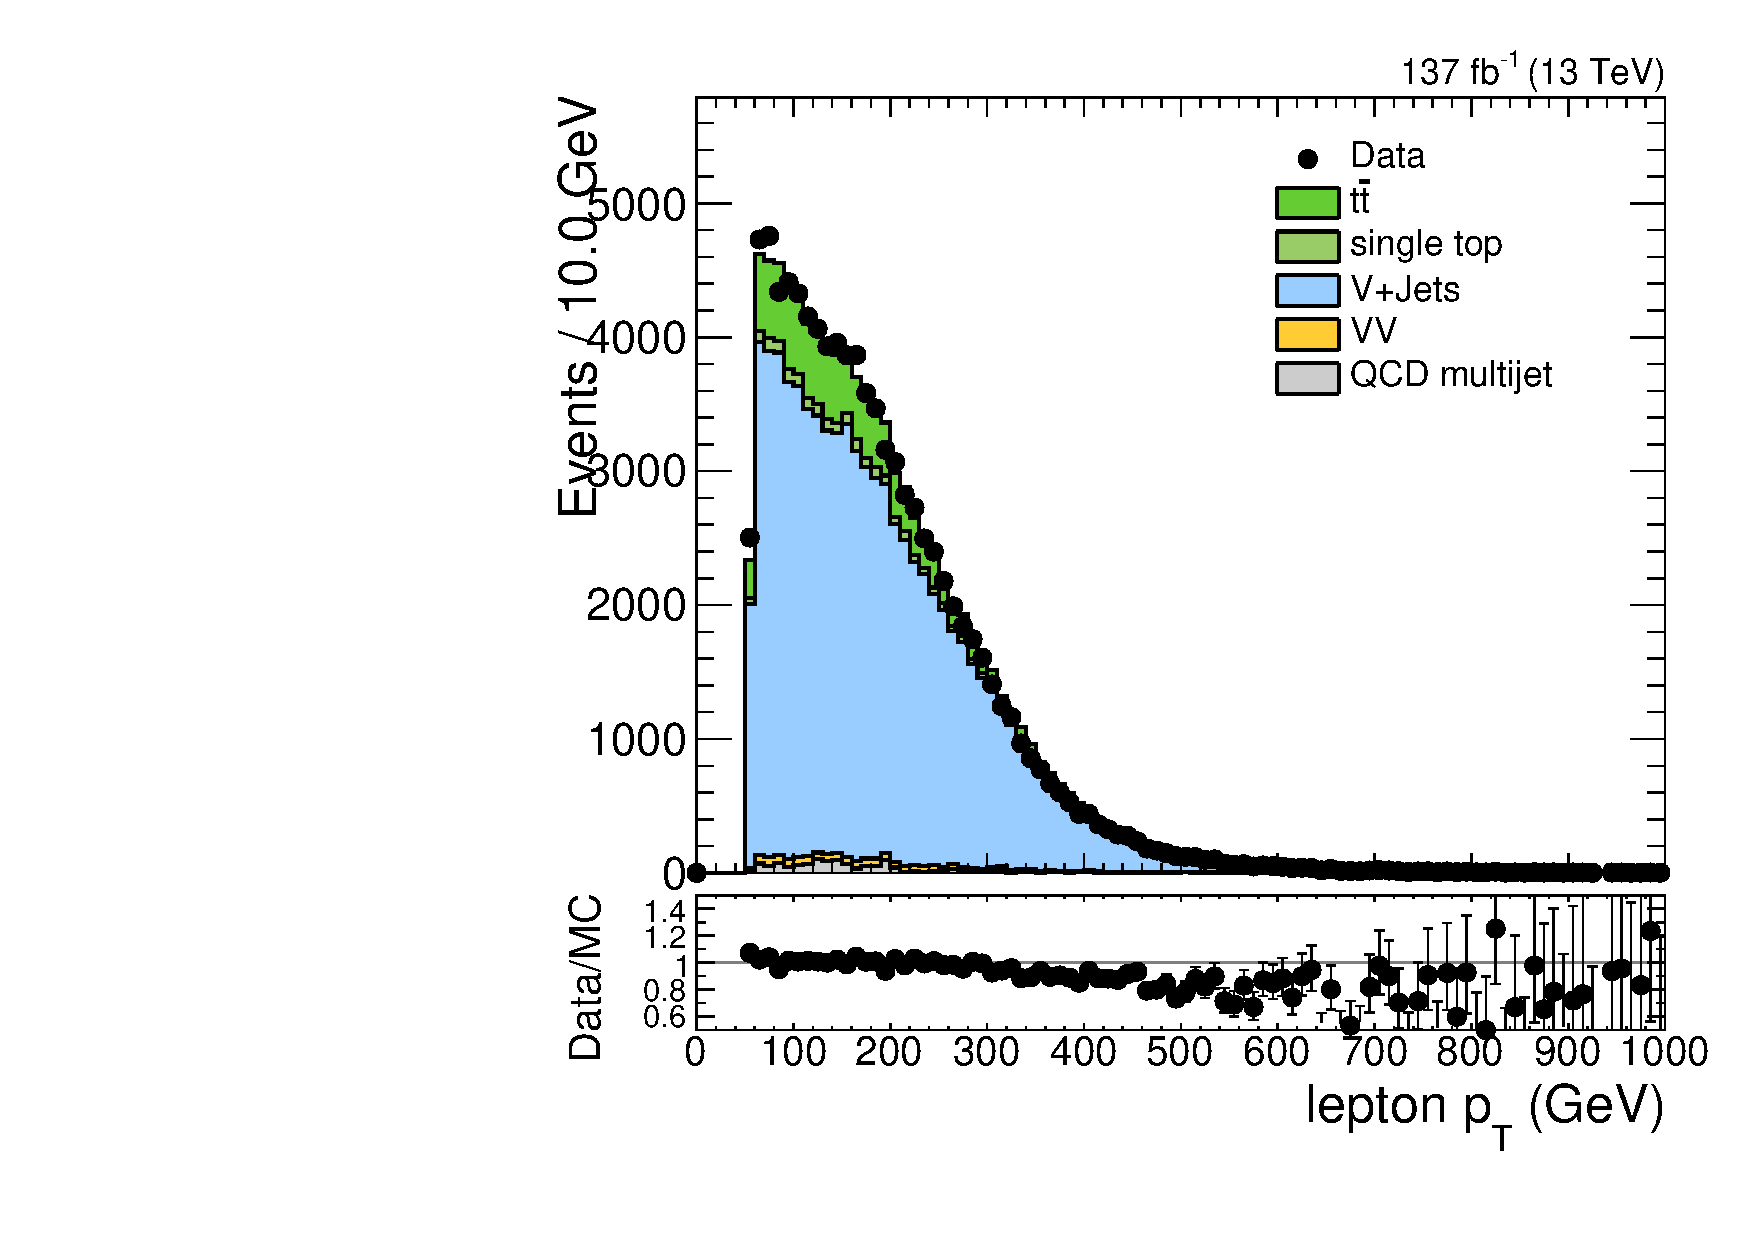
\includegraphics[width=0.3\textwidth]{fig/controlPlots/SB_b1_mu_allP_allC_allD_Run2_lnujj_l1_l_pt.pdf}
  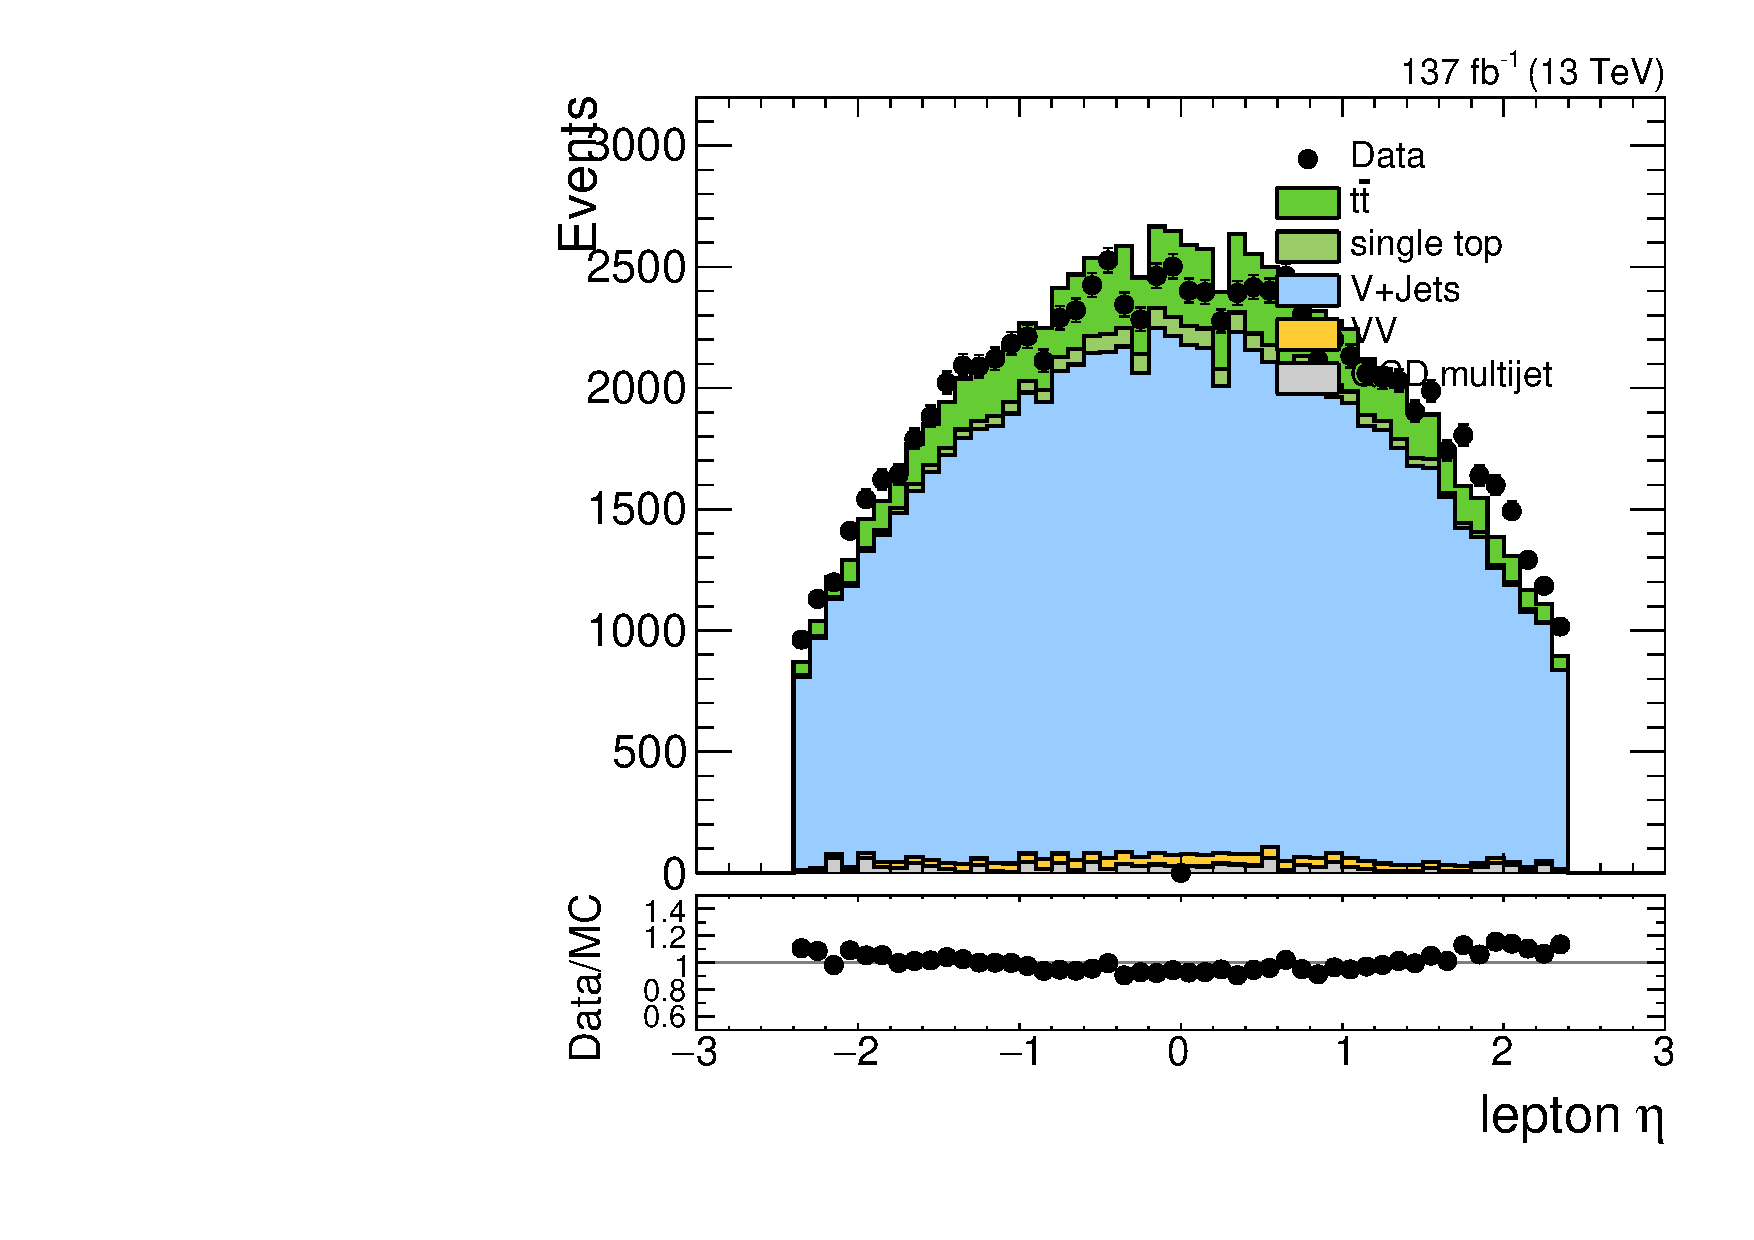
\includegraphics[width=0.3\textwidth]{fig/controlPlots/SB_b1_mu_allP_allC_allD_Run2_lnujj_l1_l_eta.pdf}
  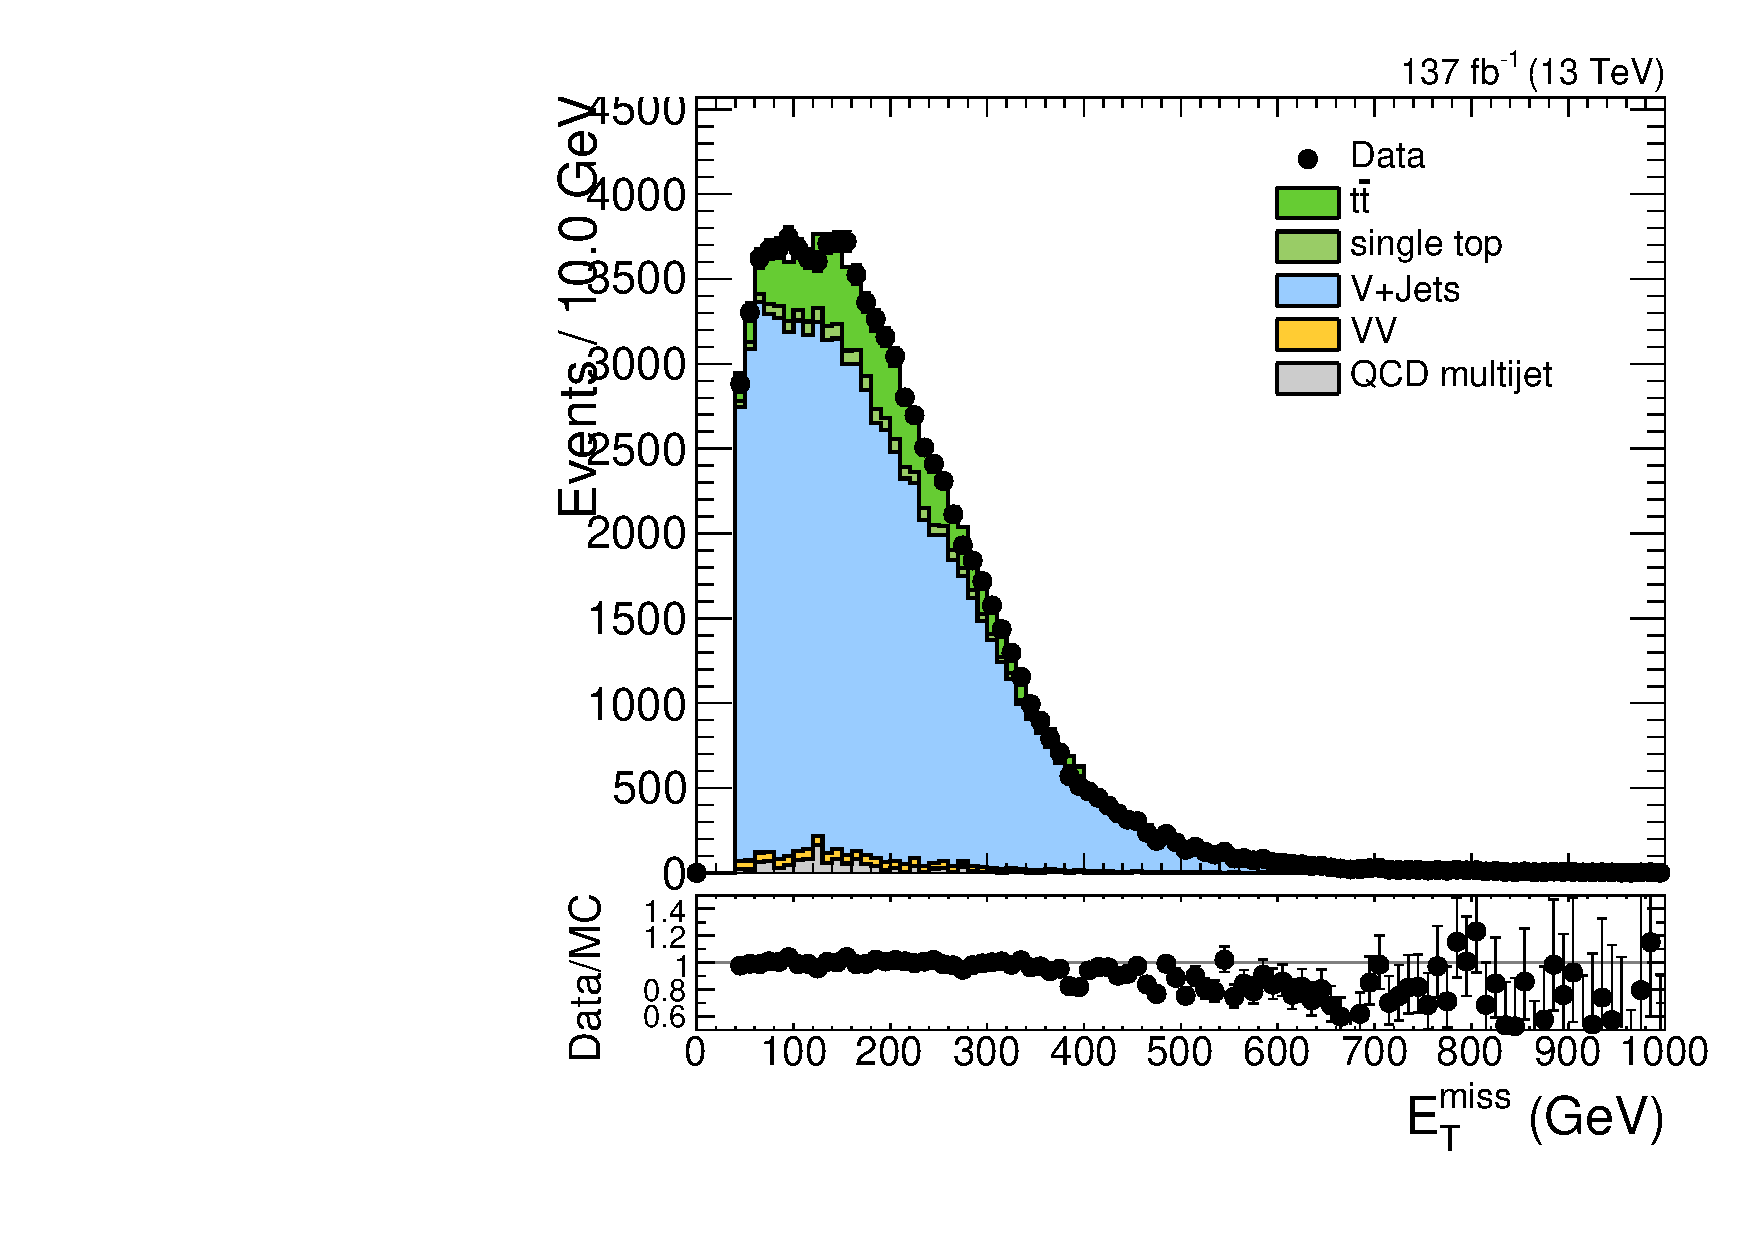
\includegraphics[width=0.3\textwidth]{fig/controlPlots/SB_b1_mu_allP_allC_allD_Run2_met_pt.pdf}\\
  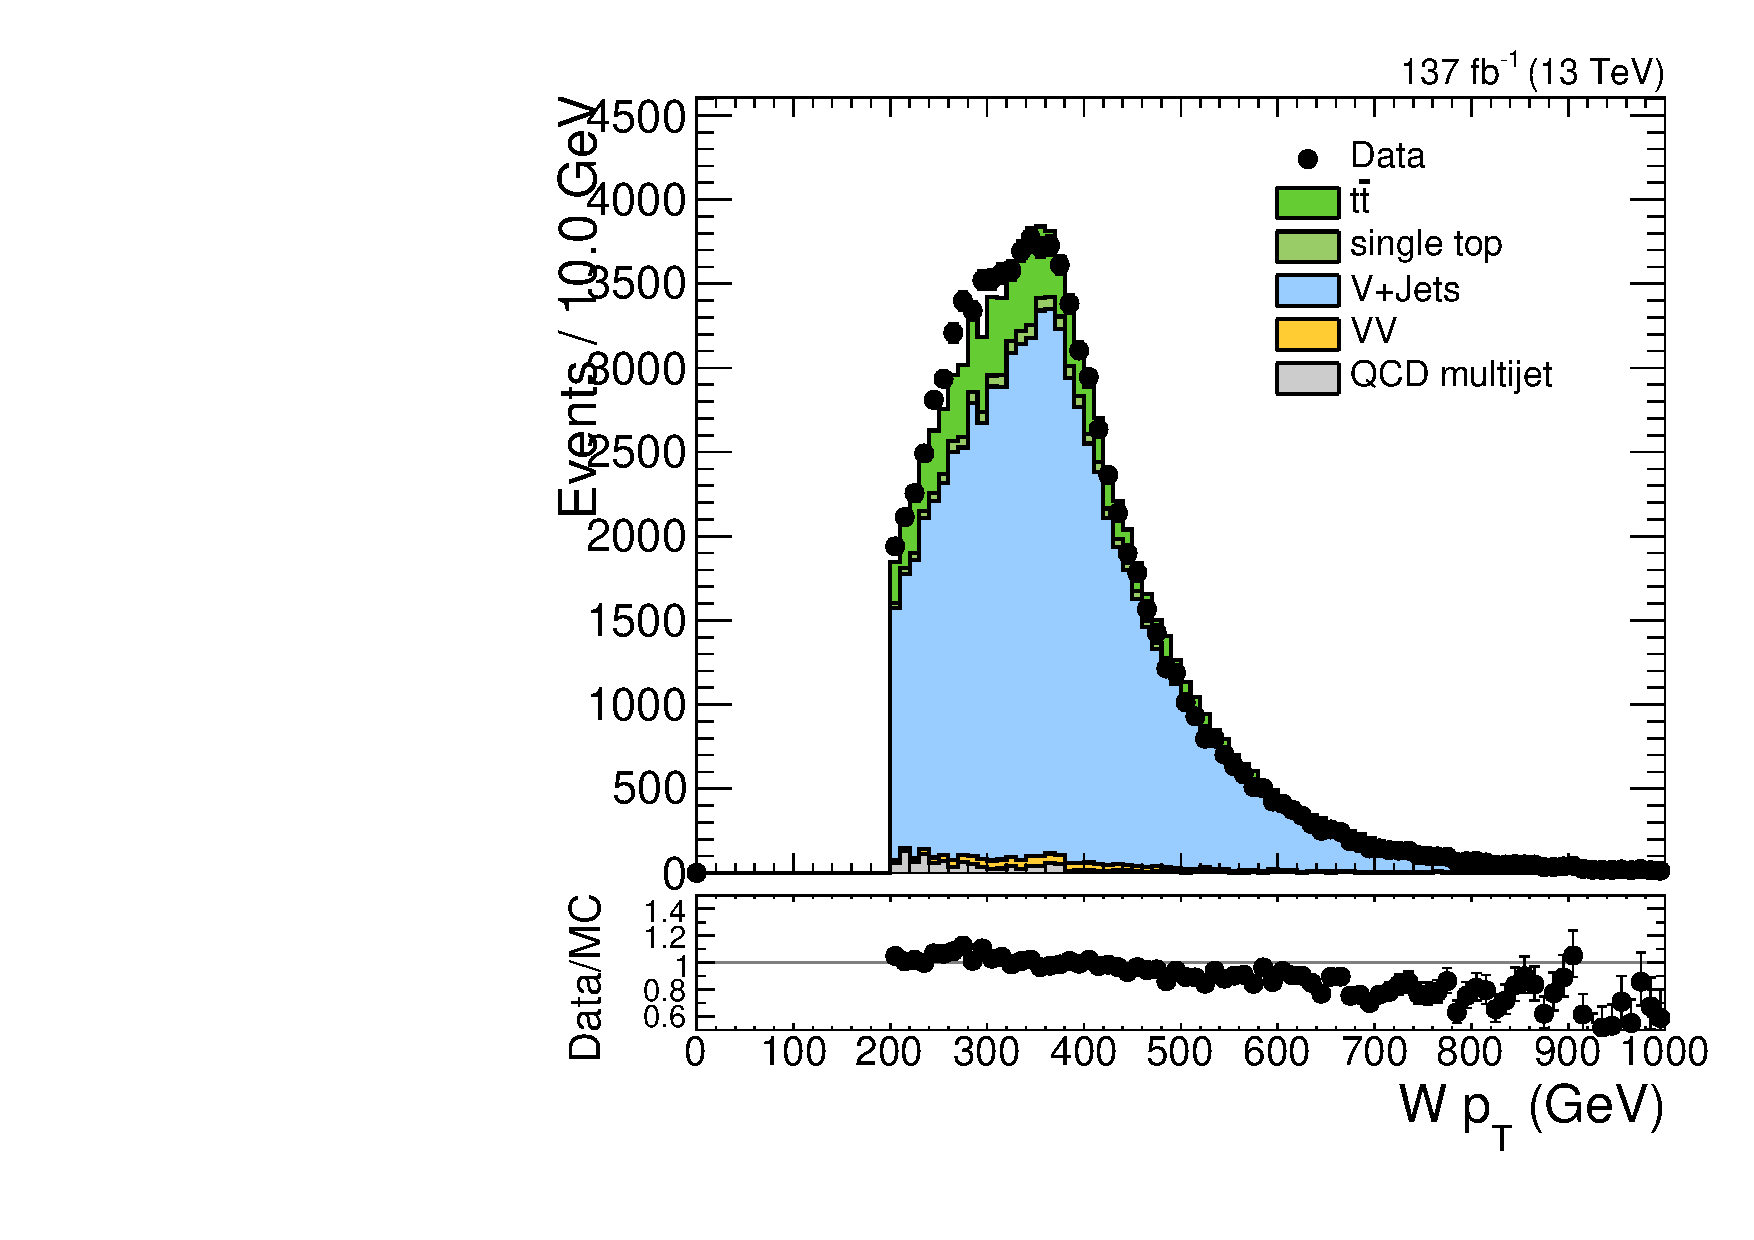
\includegraphics[width=0.3\textwidth]{fig/controlPlots/SB_b1_mu_allP_allC_allD_Run2_lnujj_l1_pt.pdf}
  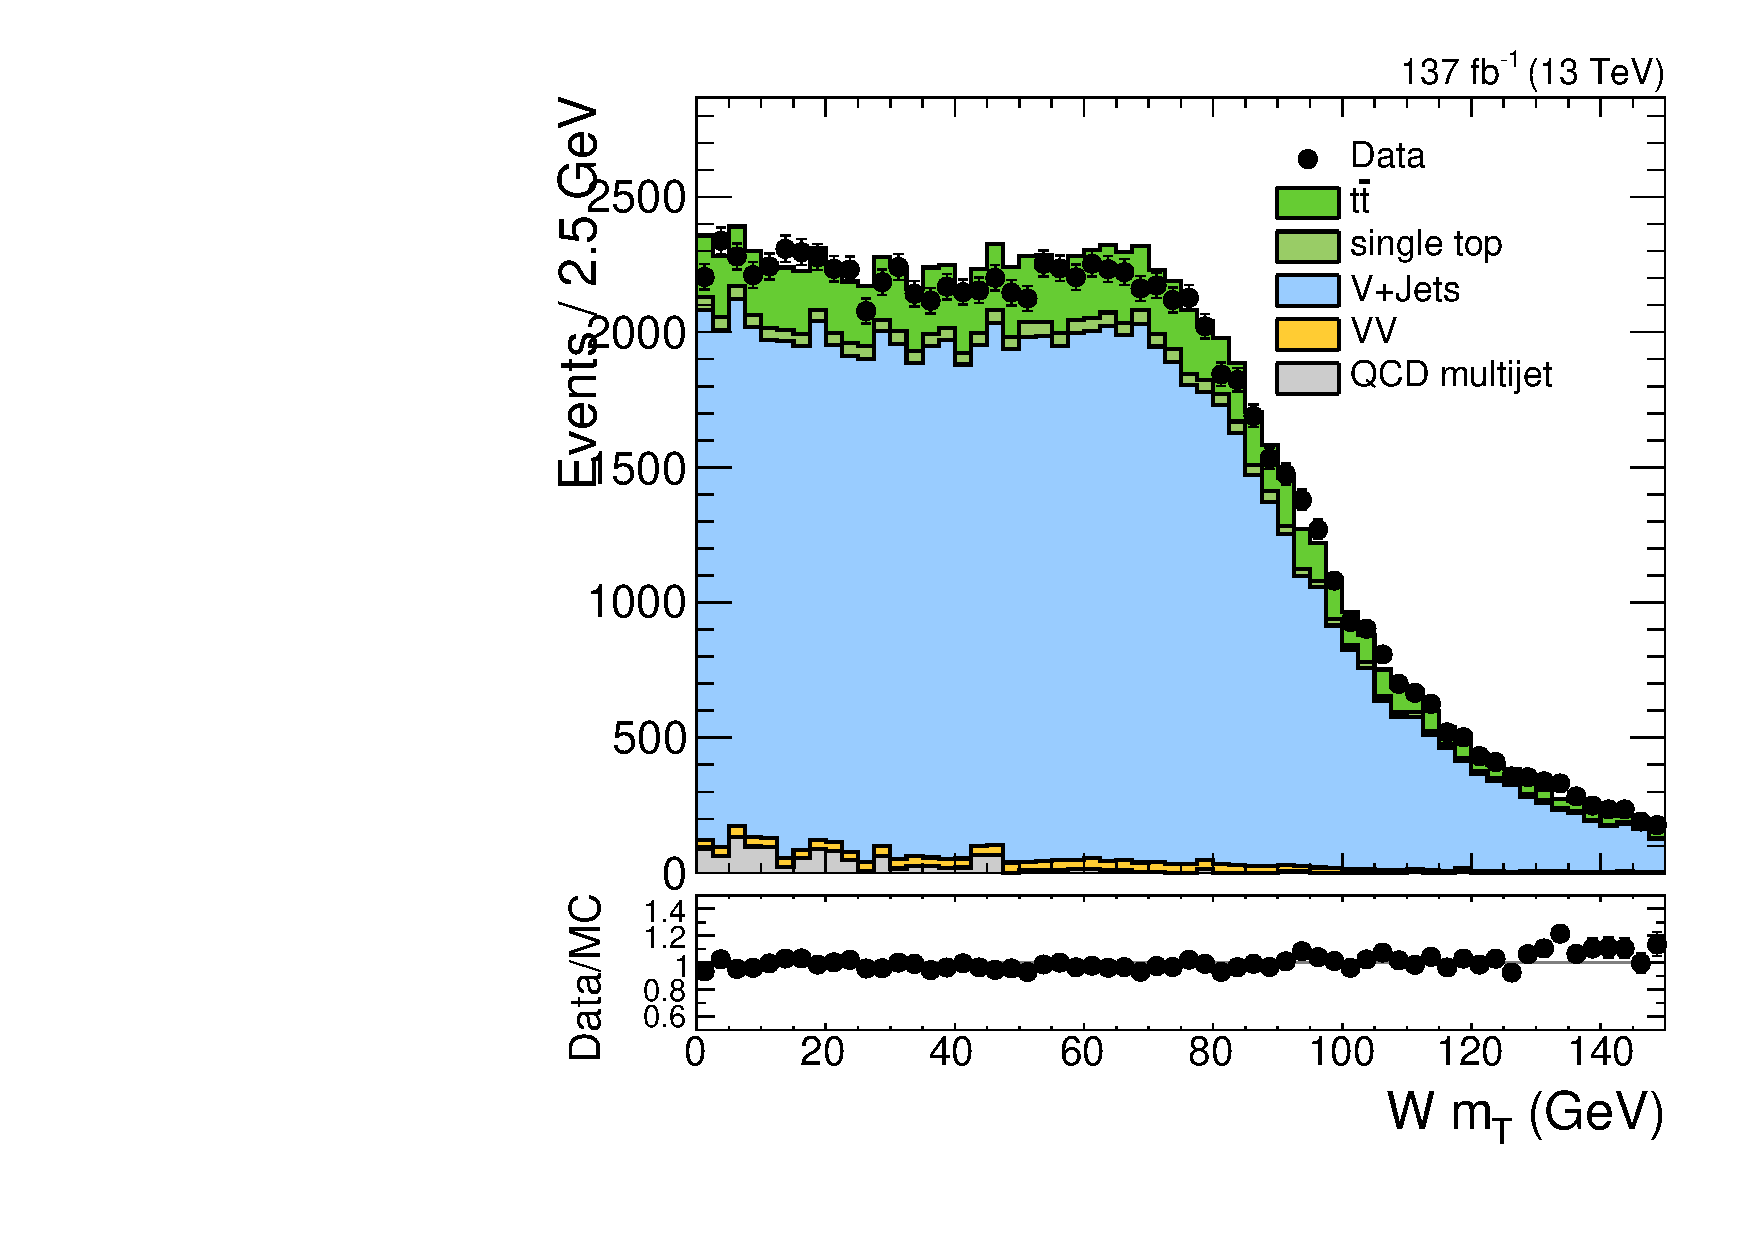
\includegraphics[width=0.3\textwidth]{fig/controlPlots/SB_b1_mu_allP_allC_allD_Run2_lnujj_l1_mt.pdf}
  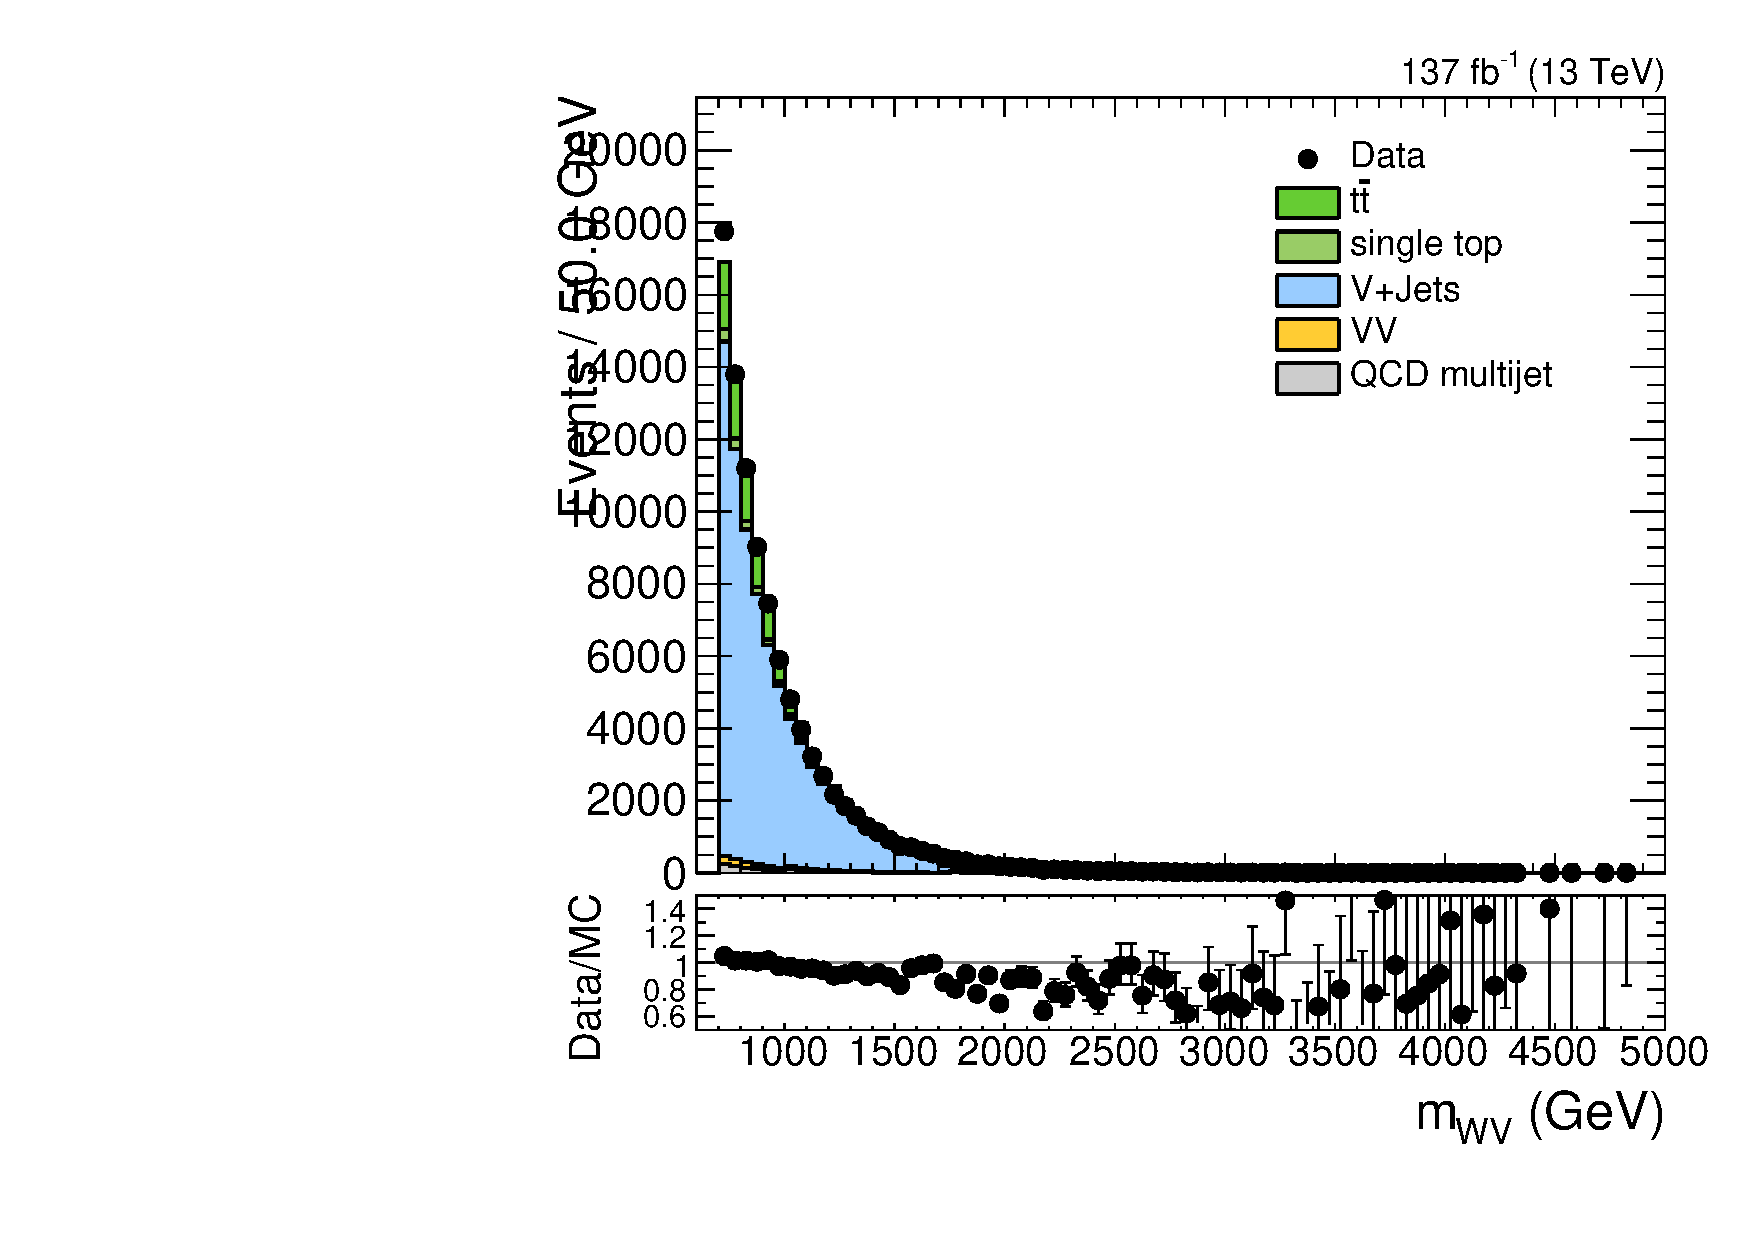
\includegraphics[width=0.3\textwidth]{fig/controlPlots/SB_b1_mu_allP_allC_allD_Run2_mWV.pdf}
  \caption{
    Comparison plots between data and MC from Run 2 for different \Wlep-related observables, in the muon channel of the jet mass sideband.
    Top row: lepton \pt, lepton $\eta$, \ptmiss.
    Bottom row: \pt of the leptonic $W^\pm$, transverse mass of the leptonic $W^\pm$, diboson invariant mass.
  }
  \label{fig:SB_controlPlotsRun2_1}
\end{figure}

\begin{figure}[htbp]
  \centering
  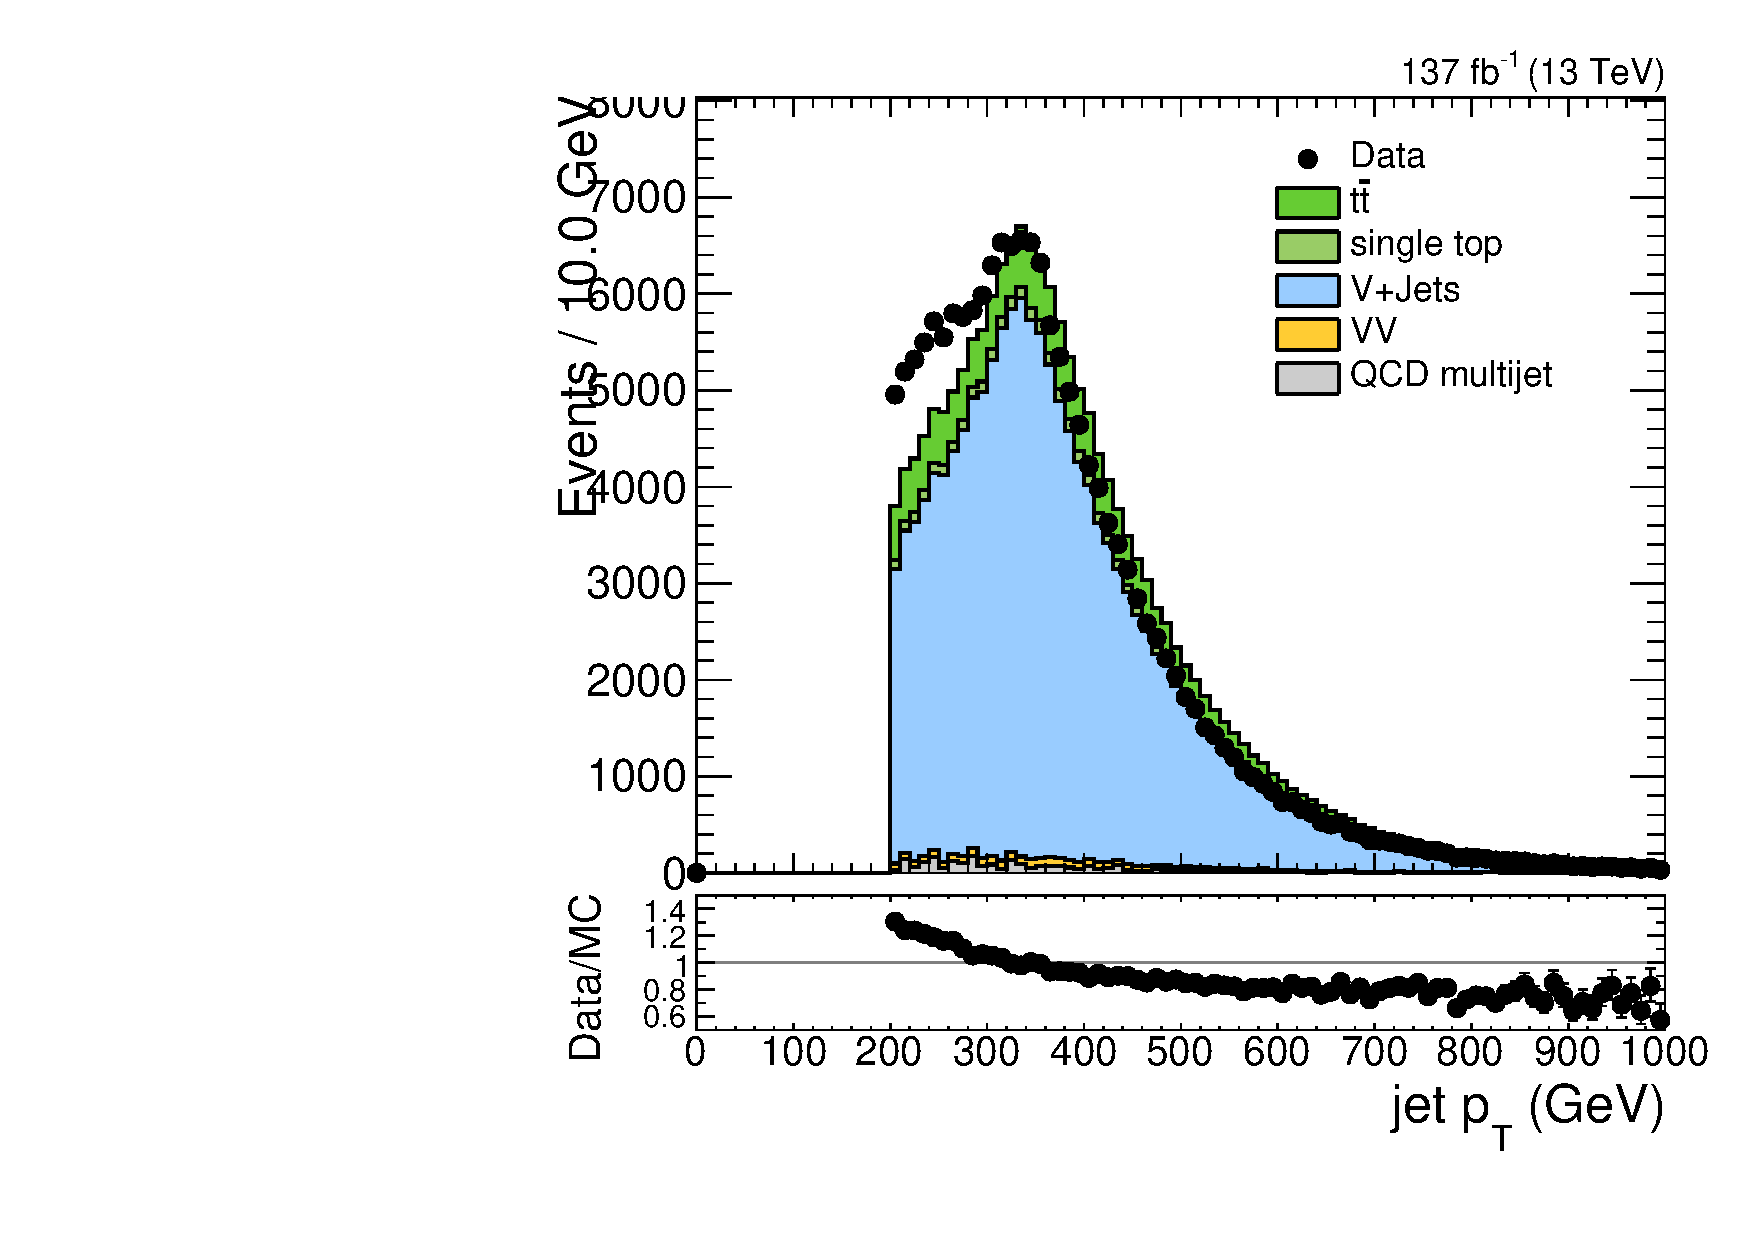
\includegraphics[width=0.3\textwidth]{fig/controlPlots/SB_b1_allL_allP_allC_allD_Run2_lnujj_l2_pt.pdf}
  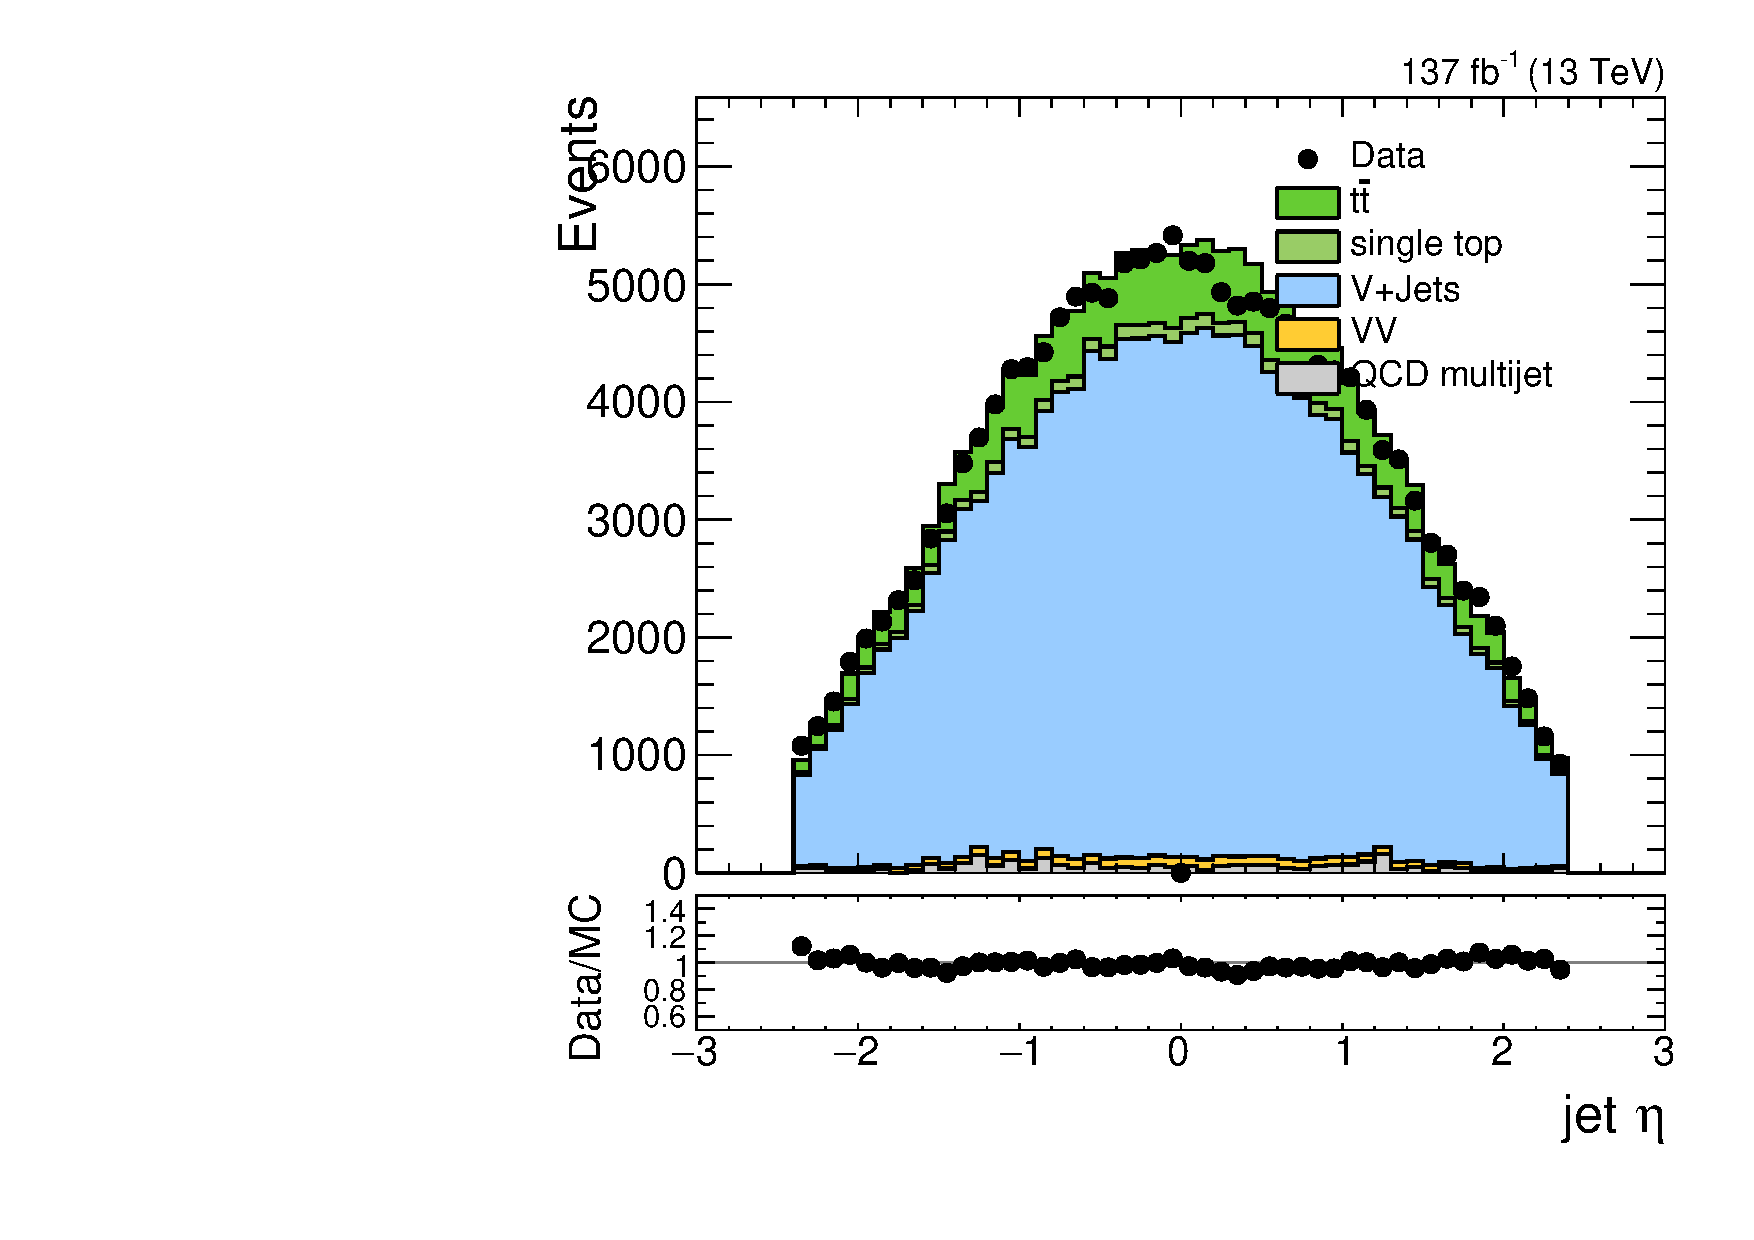
\includegraphics[width=0.3\textwidth]{fig/controlPlots/SB_b1_allL_allP_allC_allD_Run2_lnujj_l2_eta.pdf}
  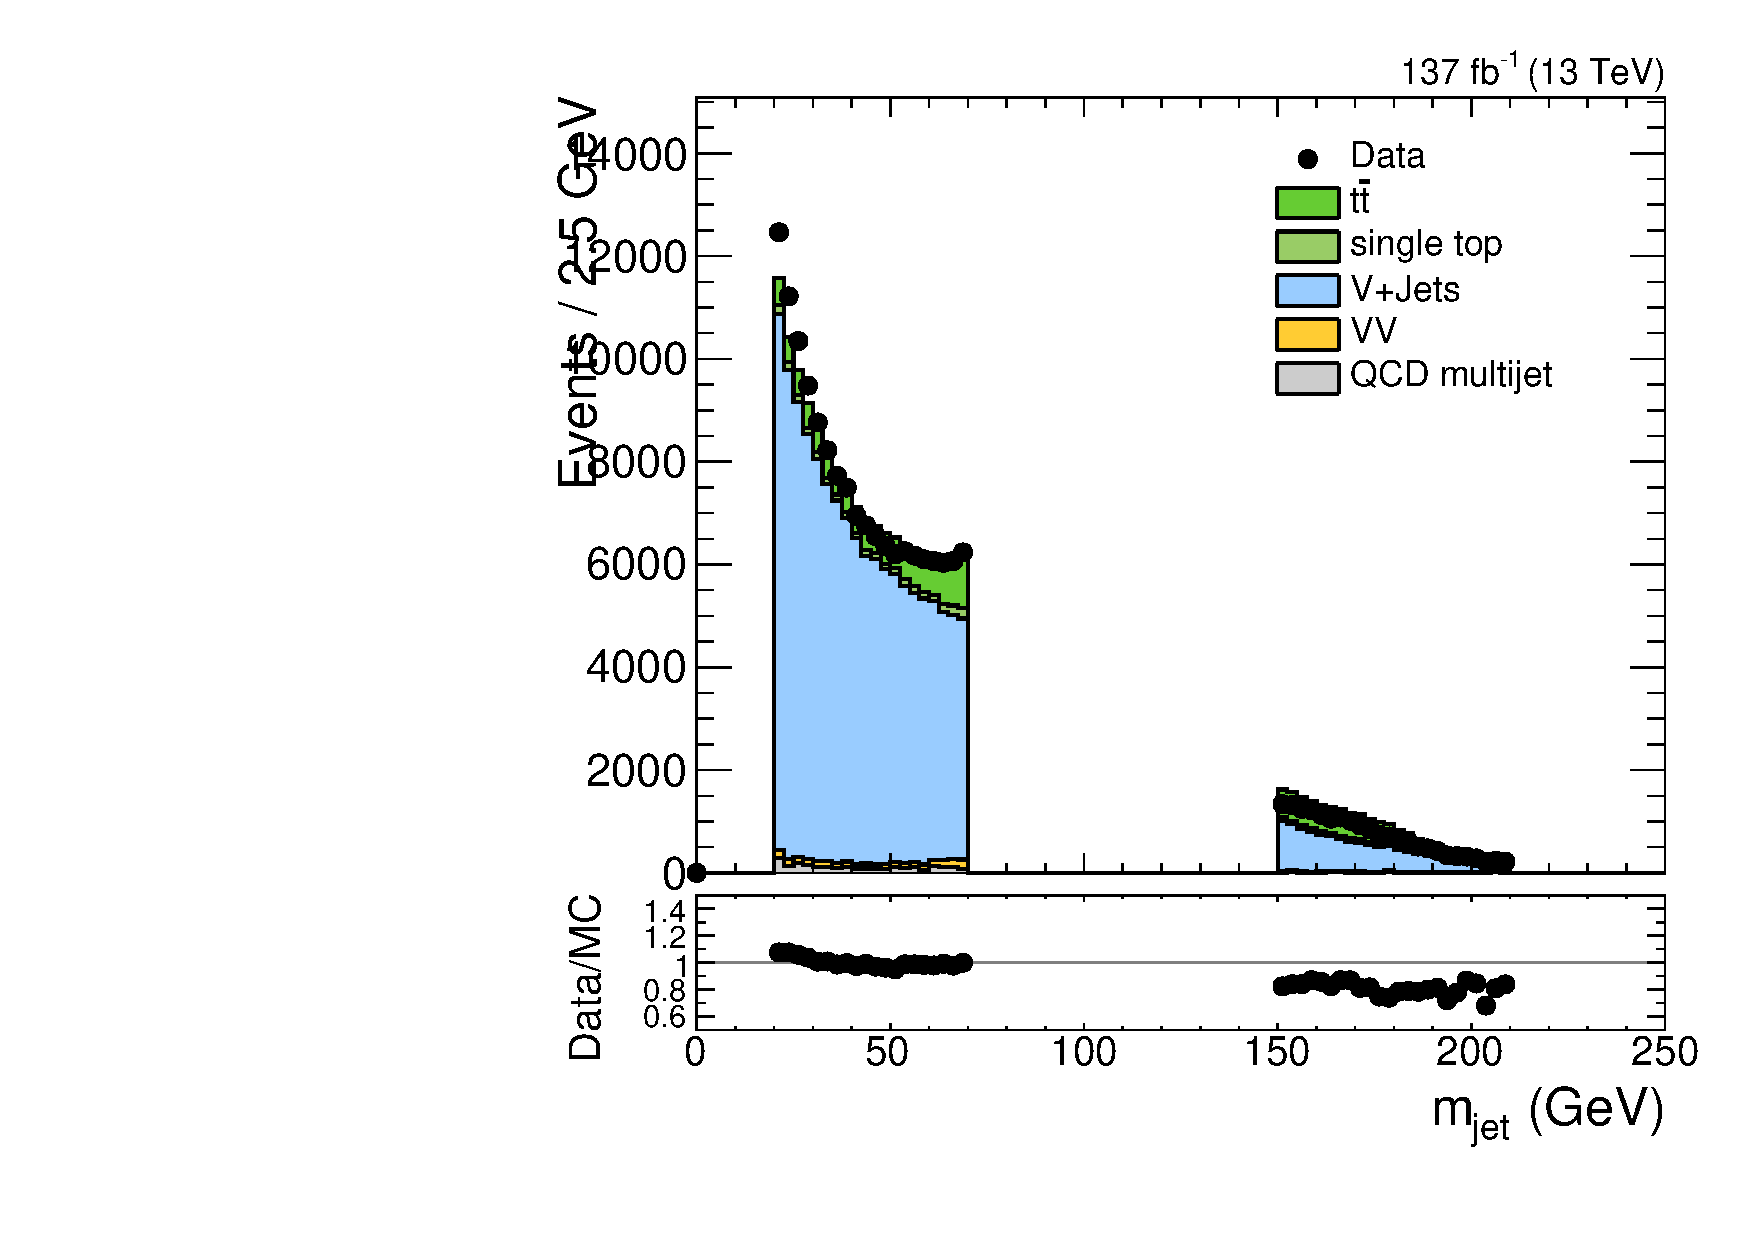
\includegraphics[width=0.3\textwidth]{fig/controlPlots/SB_b1_allL_allP_allC_allD_Run2_mjet.pdf}\\
  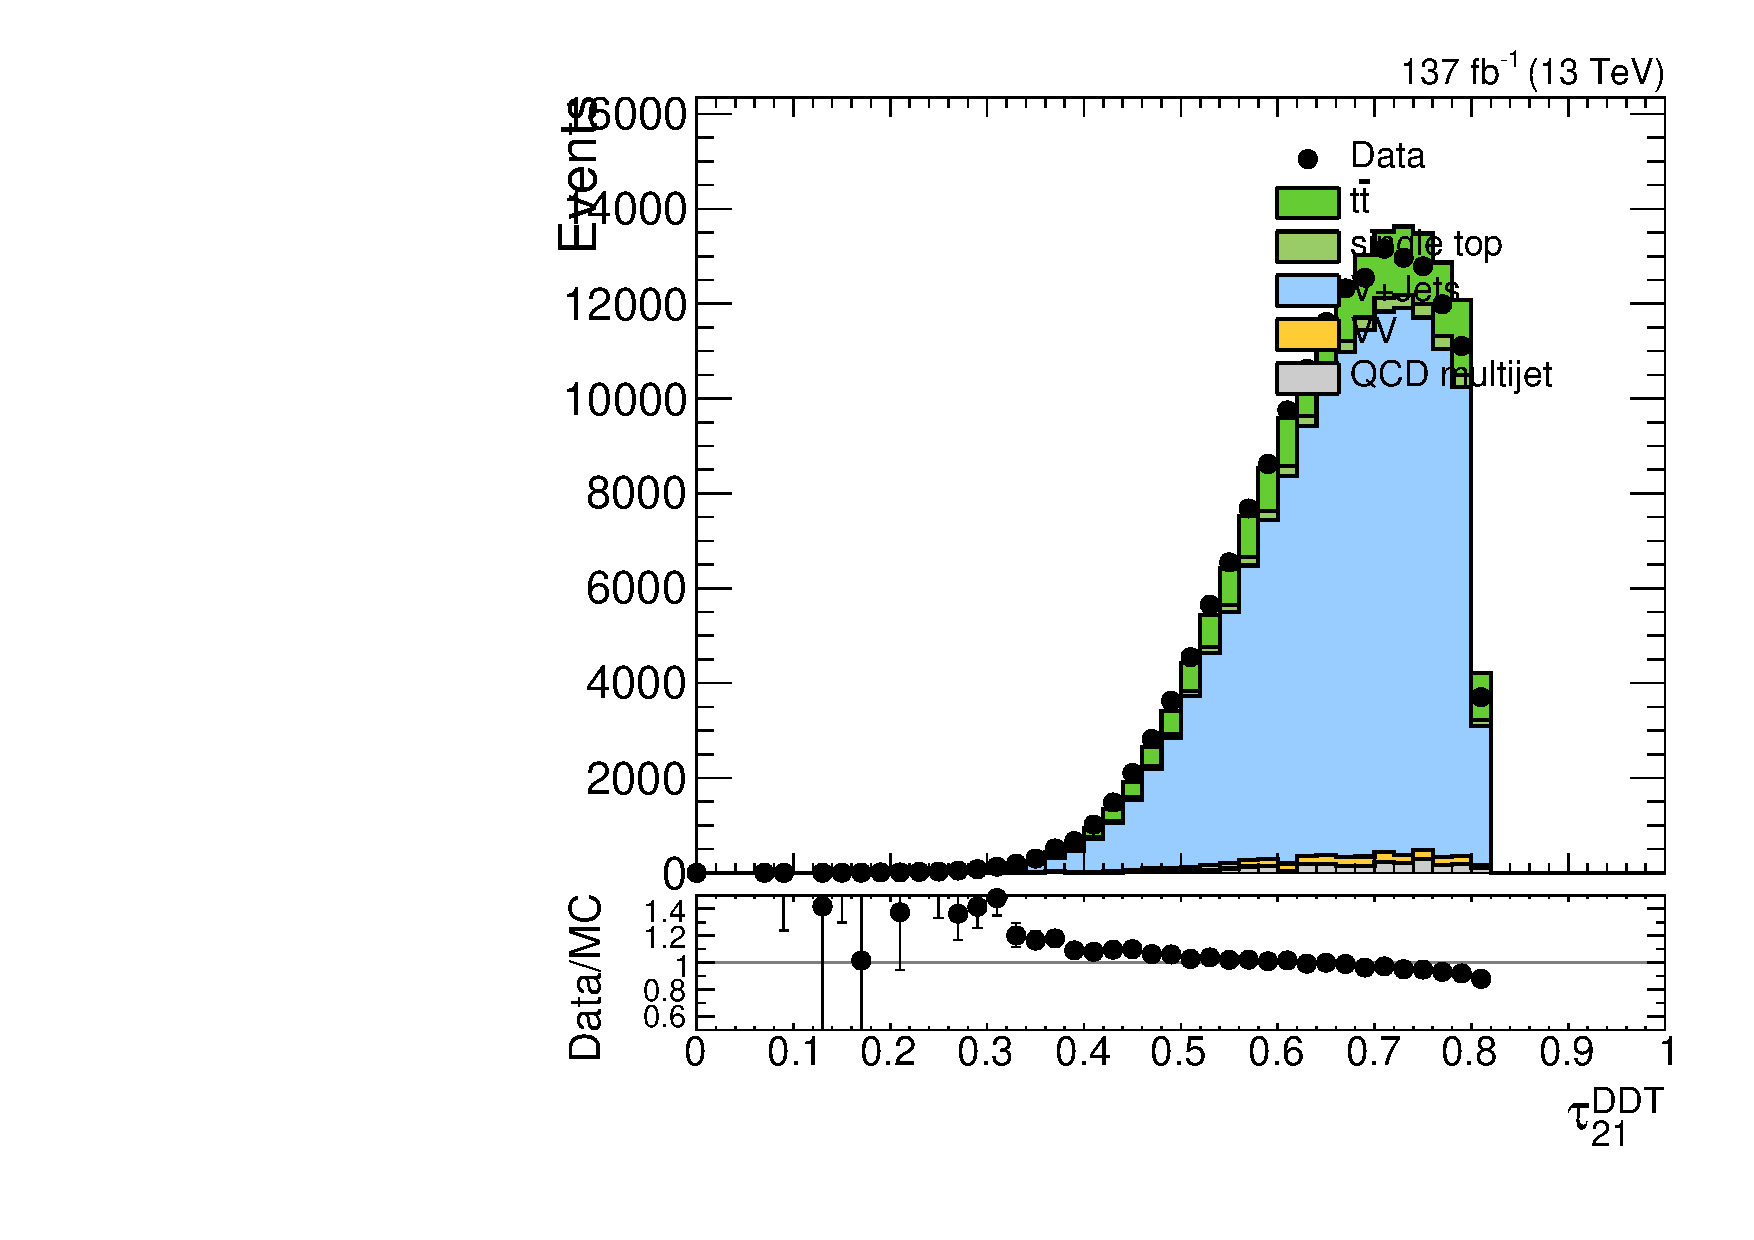
\includegraphics[width=0.3\textwidth]{fig/controlPlots/SB_b1_allL_allP_allC_allD_Run2_tau21DDT.pdf}
  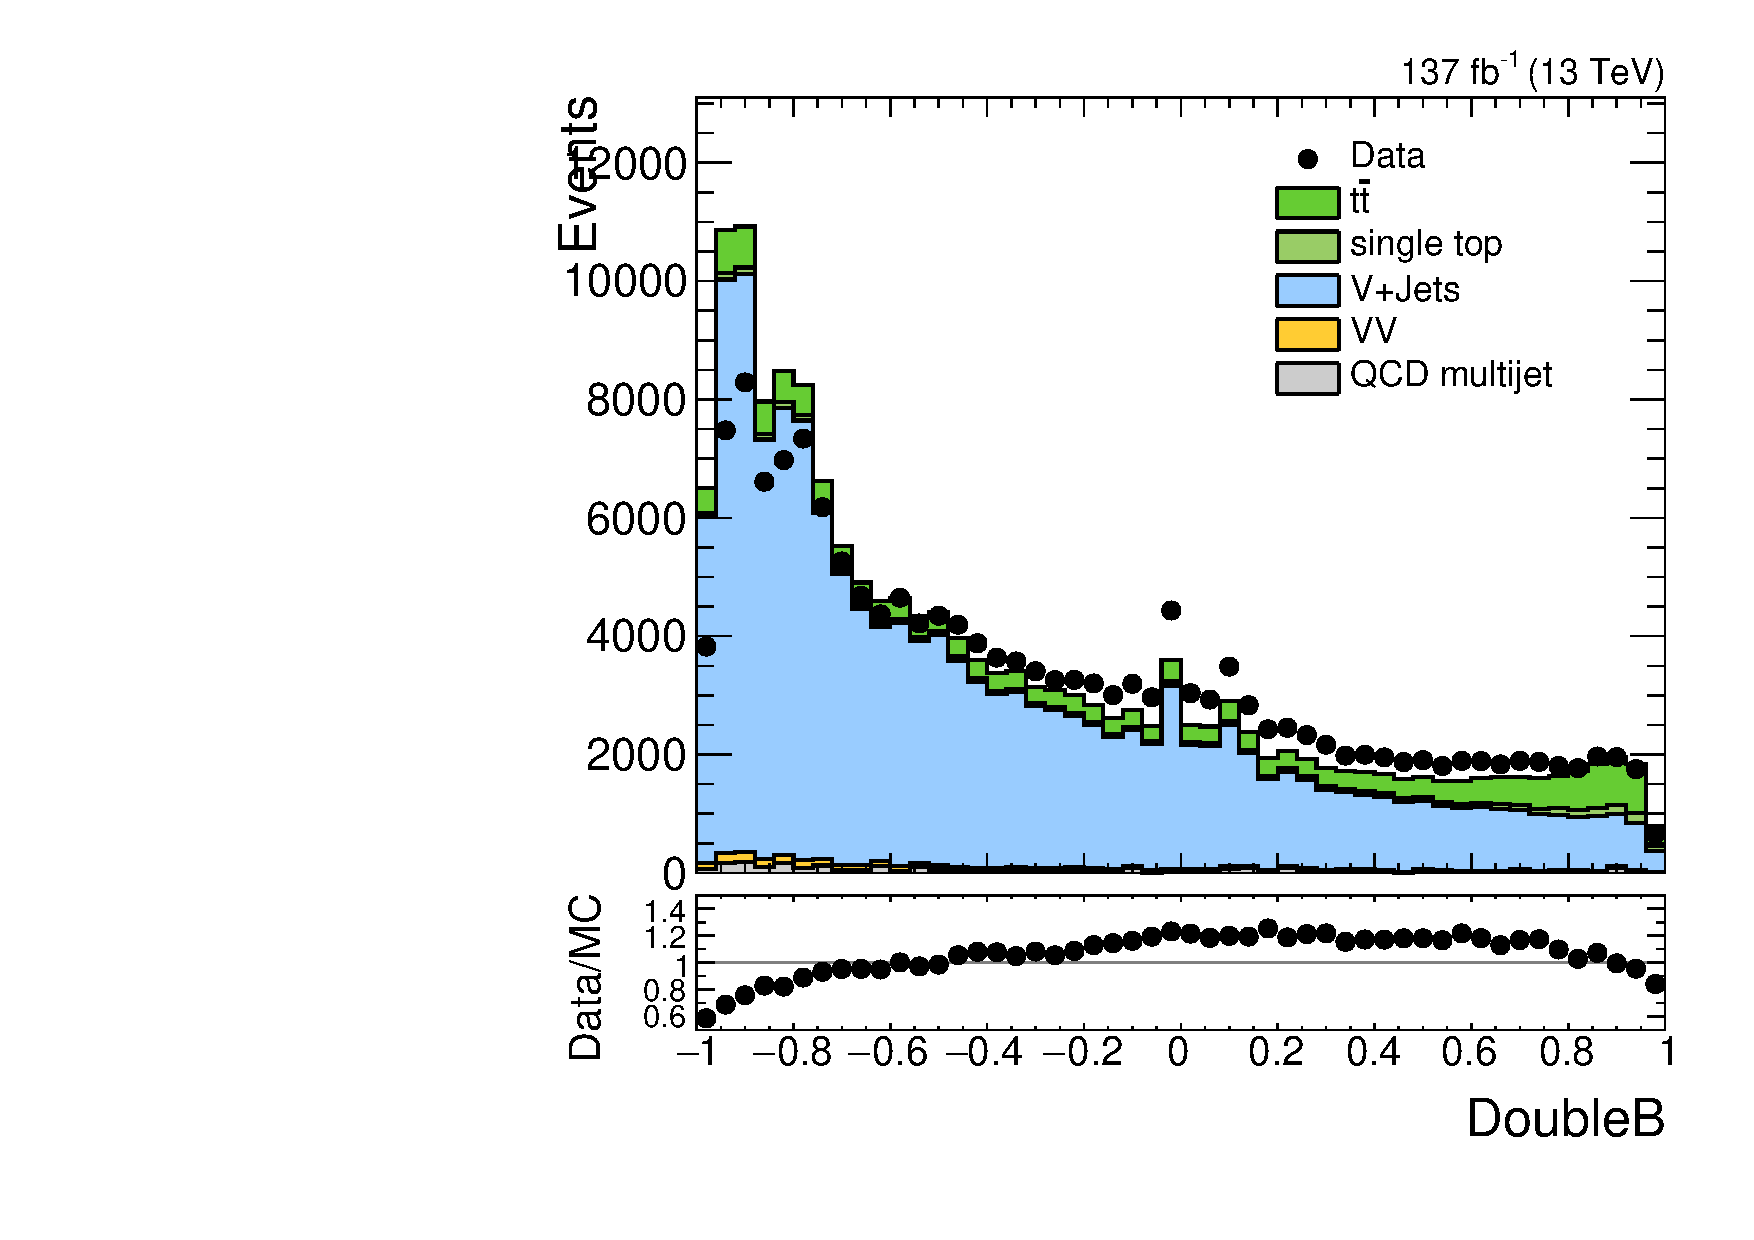
\includegraphics[width=0.3\textwidth]{fig/controlPlots/SB_b1_allL_allP_allC_allD_Run2_DoubleB.pdf}
  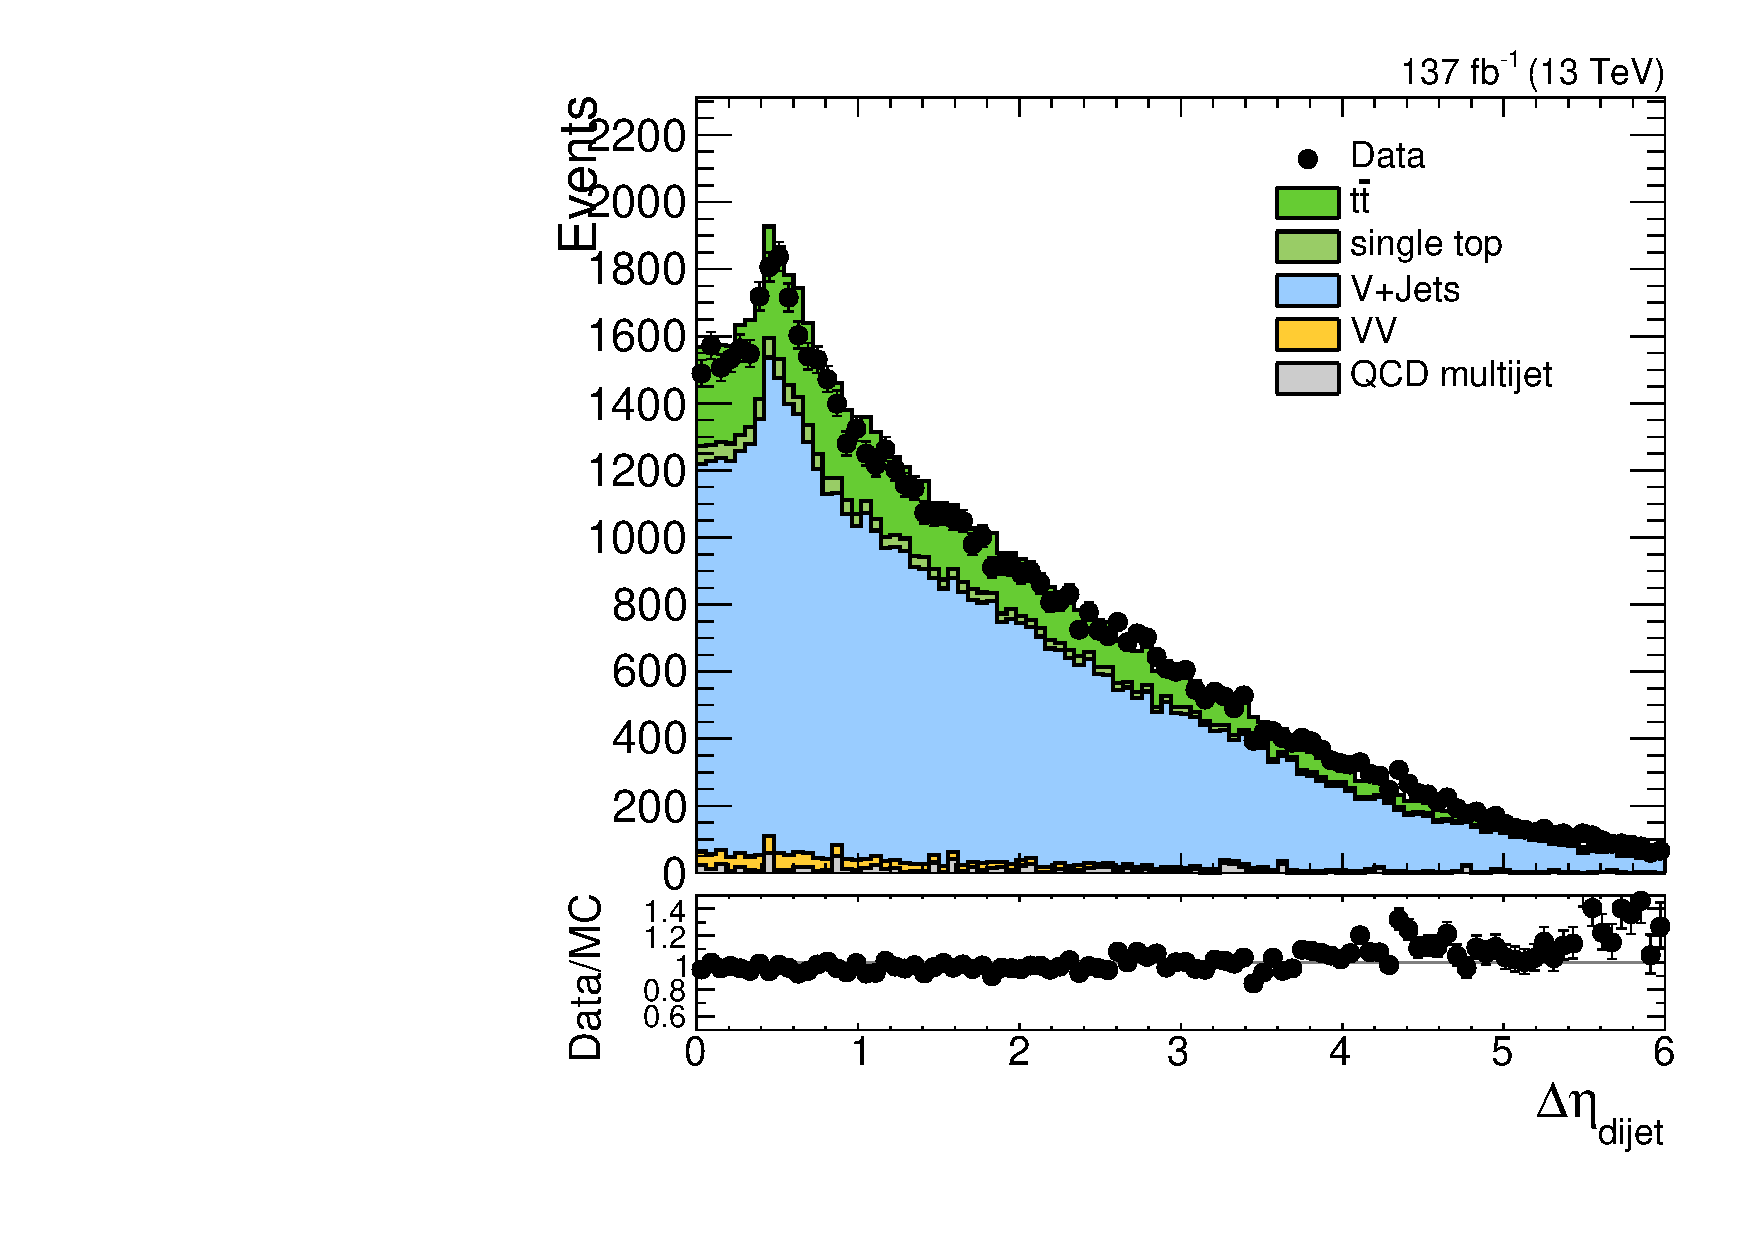
\includegraphics[width=0.3\textwidth]{fig/controlPlots/SB_b1_allL_allP_allC_allD_Run2_lnujj_vbfDEta.pdf}\\
  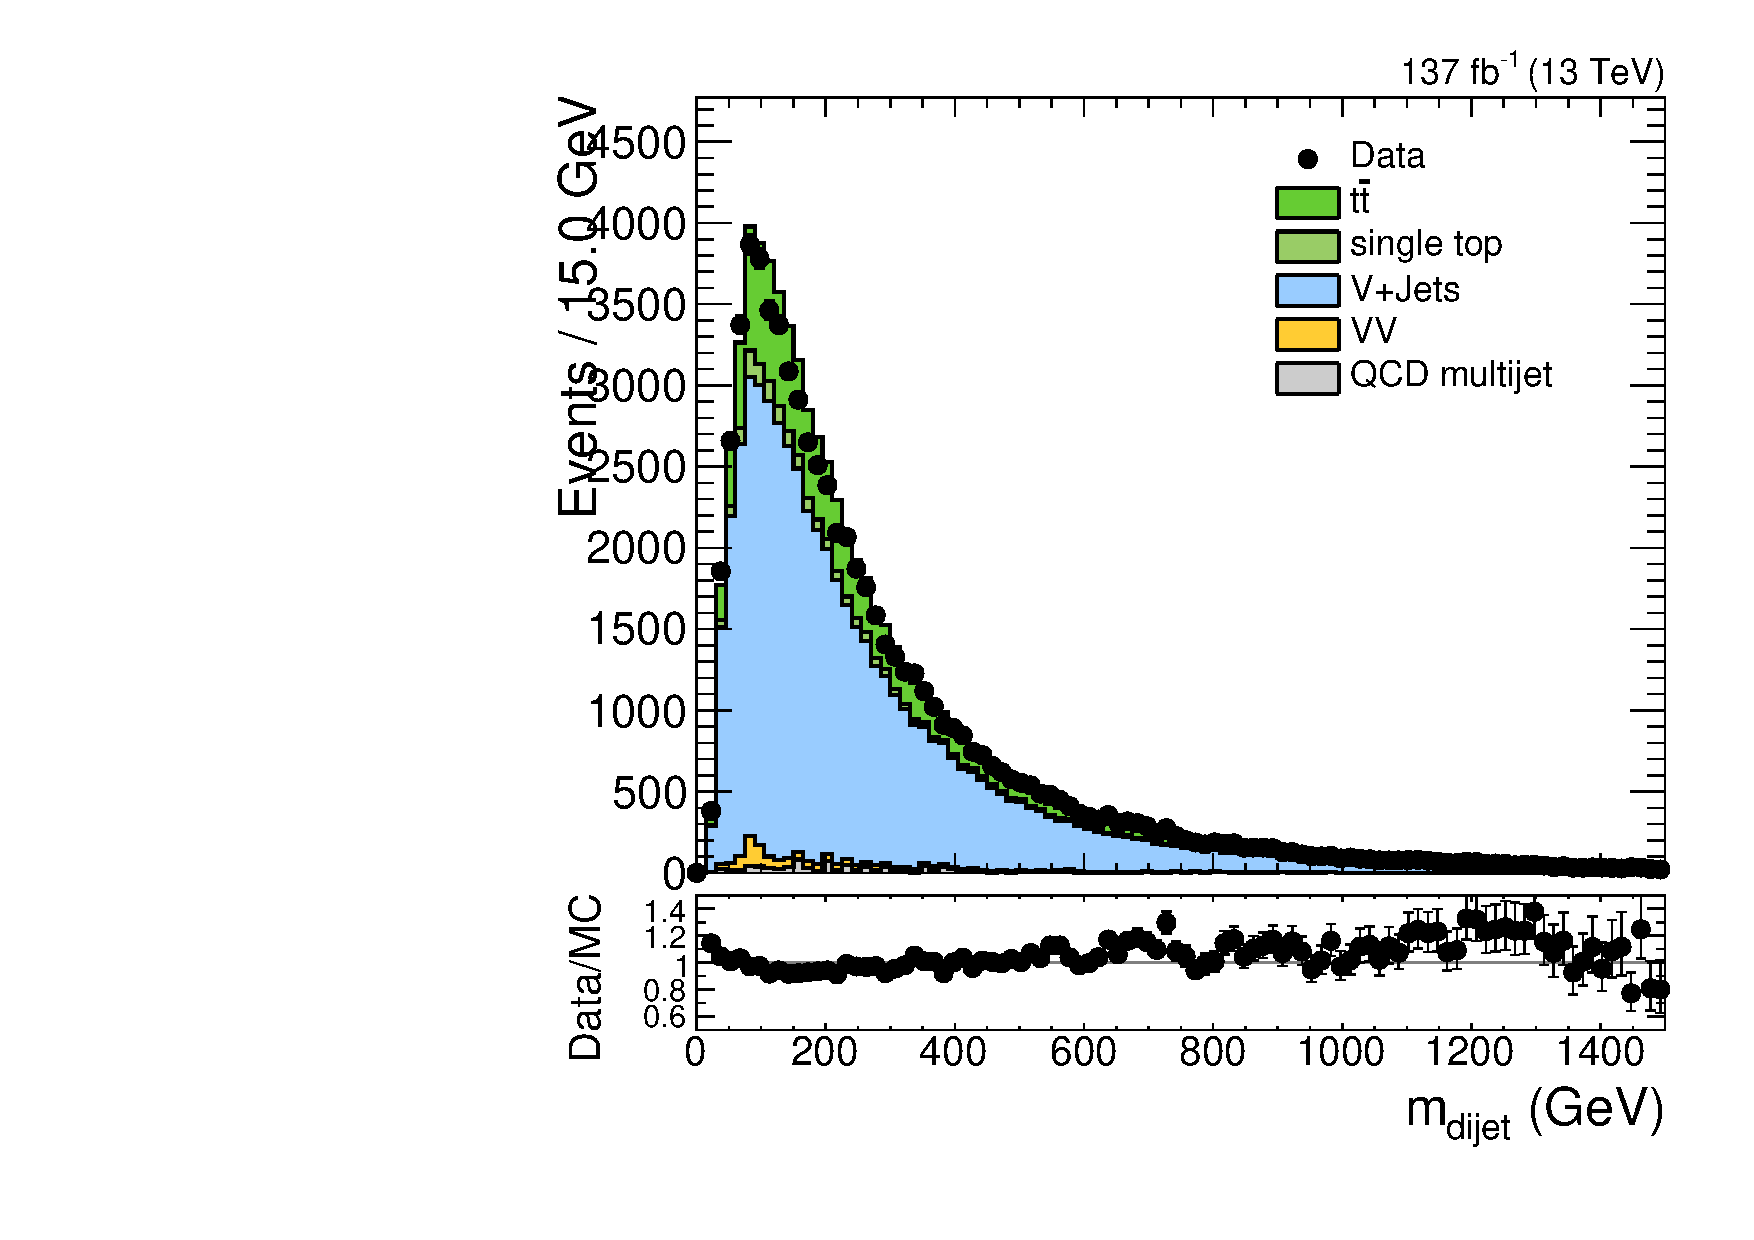
\includegraphics[width=0.3\textwidth]{fig/controlPlots/SB_b1_allL_allP_allC_allD_Run2_lnujj_vbfMass.pdf}
  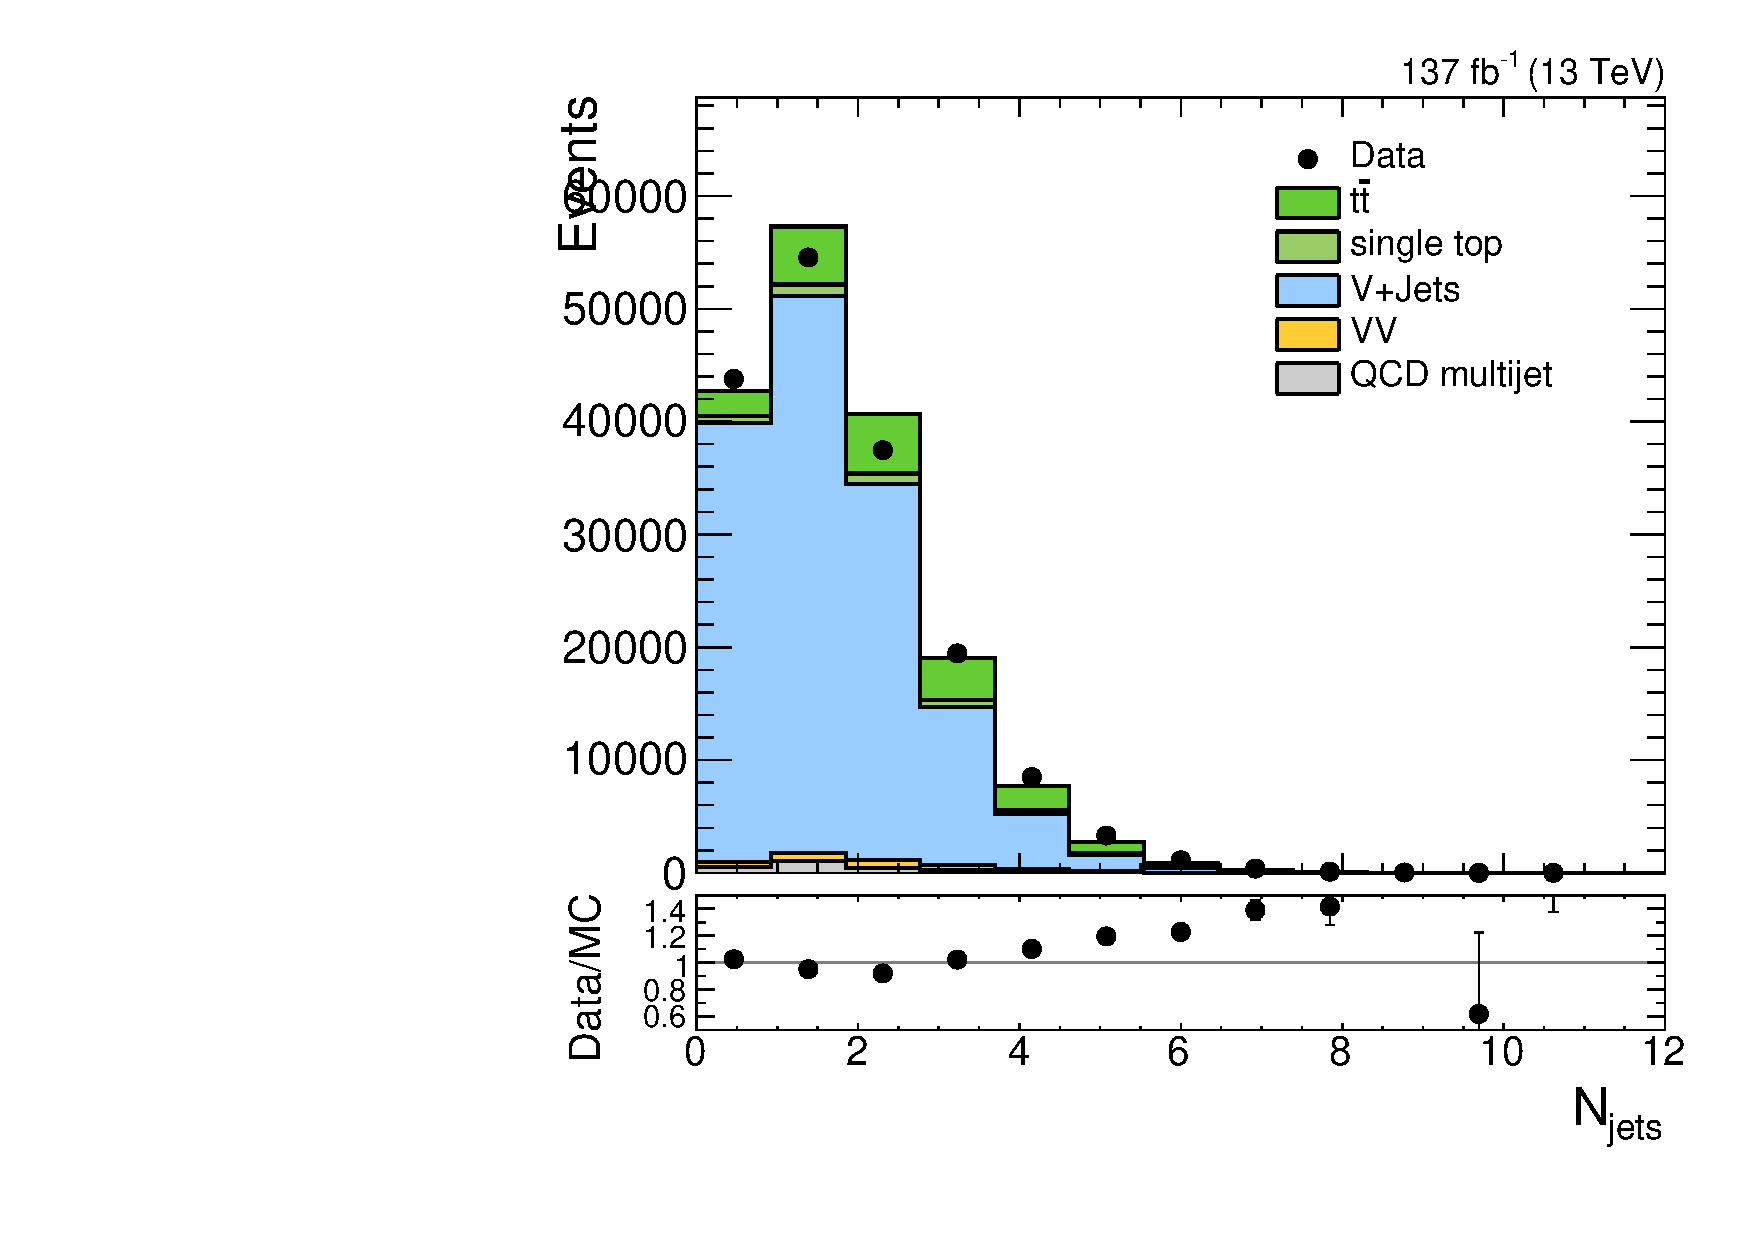
\includegraphics[width=0.3\textwidth]{fig/controlPlots/SB_b1_allL_allP_allC_allD_Run2_lnujj_nJets.pdf}
  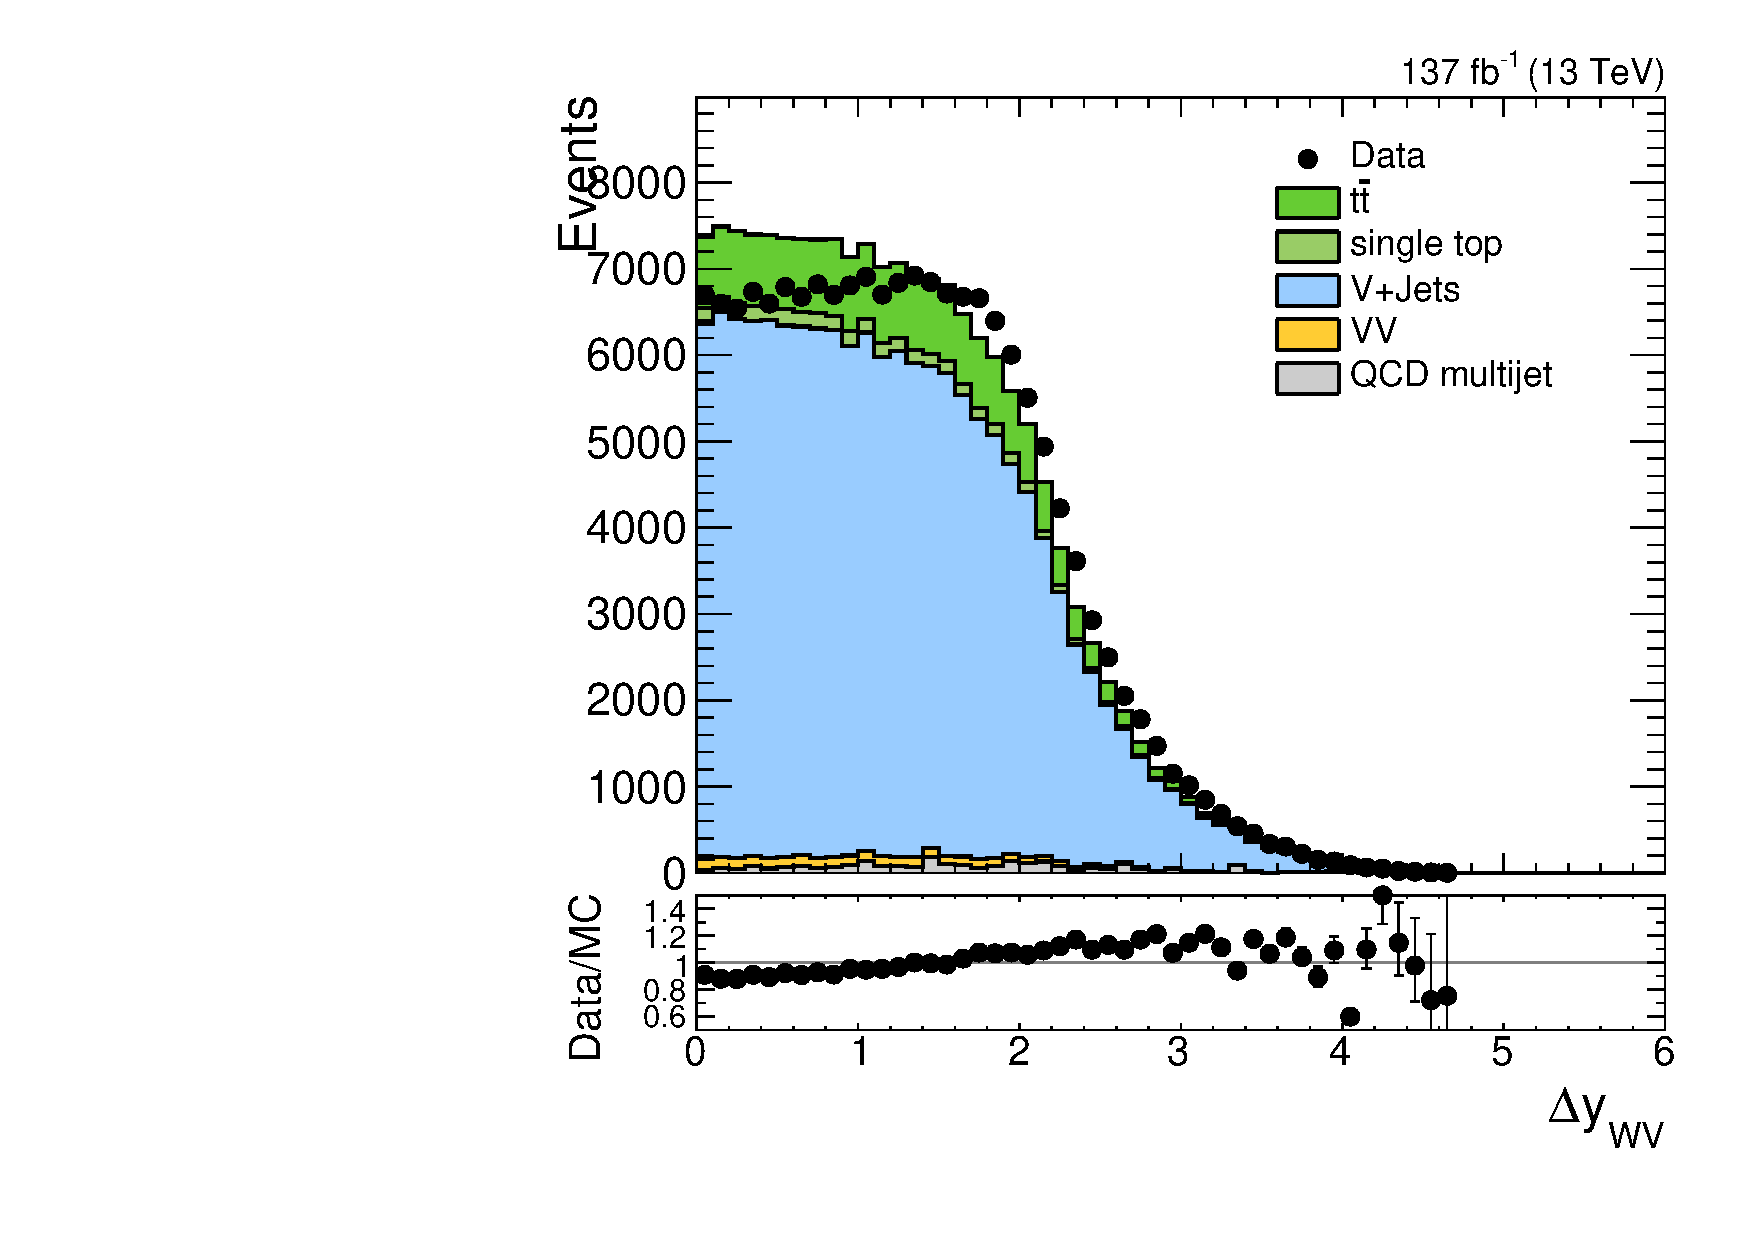
\includegraphics[width=0.3\textwidth]{fig/controlPlots/SB_b1_allL_allP_allC_allD_Run2_dy.pdf}\\
  \caption{
    Comparison plots between data and MC from Run 2 for different \Vhad and \VBF forward jet variables, in the jet mass sideband.
    Top row: \pt, $\eta$, \MJ (soft drop mass).
    Middle row: \nsubjDDT, \DoubleB tagger of the selected \Vhad candidate, separation in $\eta$ of the \VBF forward jets.
    Bottom row: invariant mass of the \VBF jets, number of selected standard jets, rapidity separation between the reconstructed bosons.
  }
  \label{fig:SB_controlPlotsRun2_2}
\end{figure}

\subsubsection{Control Plots in the Top-Enriched Control Region}

% Top-enriched control plots
Figure~\ref{fig:CR_controlPlotsRun2_1} shows control plots of lepton-related observables in the top-enriched control region, with the \pt, $\eta$, \ptmiss, \pt and transverse mass of the \Wlep candidate, and diboson invariant mass \MVV, for the $\mu$ channel.
In figure~\ref{fig:CR_controlPlotsRun2_2}, distributions of variables related to the \Vhad and \VBF forward jets are shown, such as the \pt, $\eta$, \MJ, \nsubjDDT, \DoubleB of the large-radius jet from the \Vhad candidate, \DetaVBF, \mjjVBF, \nJets, and \Dy.

\begin{figure}[htbp]
  \centering
  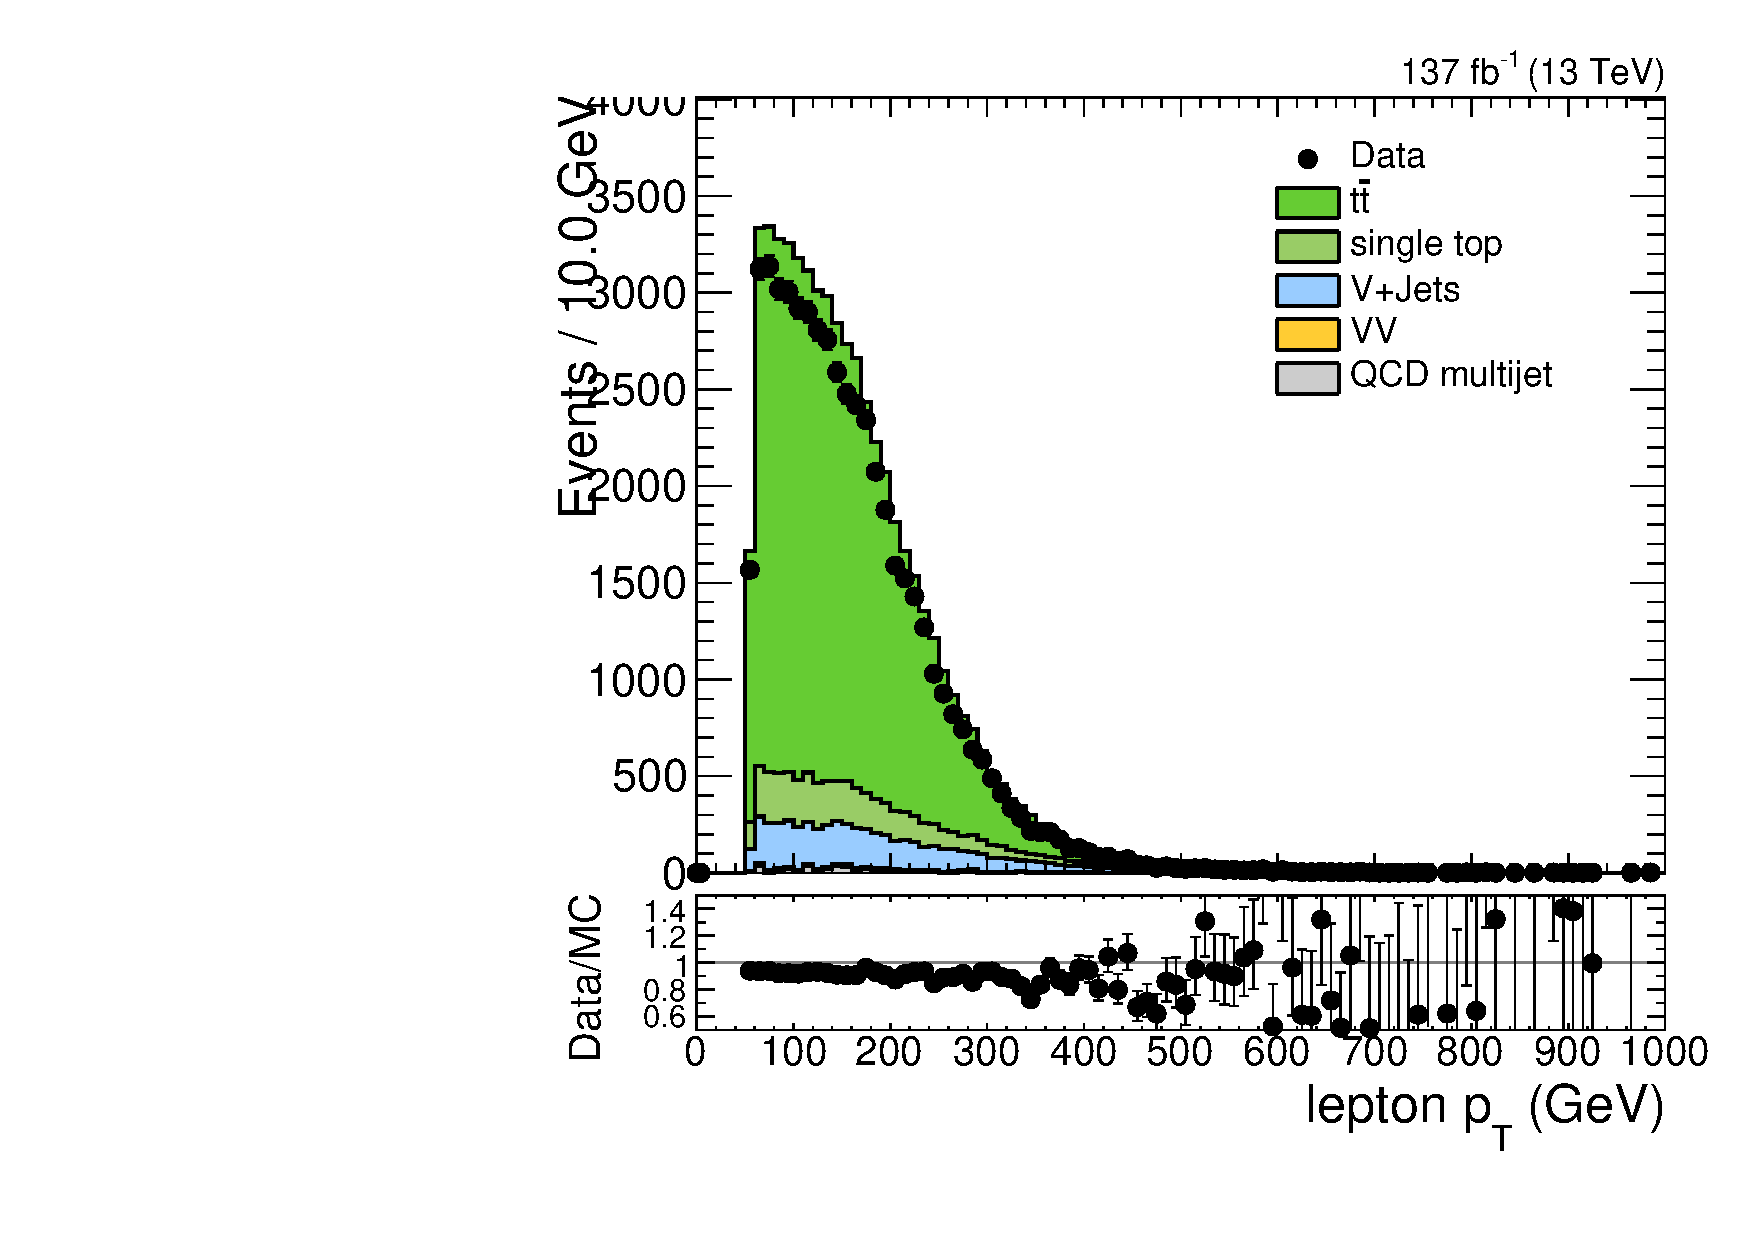
\includegraphics[width=0.3\textwidth]{fig/controlPlots/CR_b1_mu_allP_allC_allD_Run2_lnujj_l1_l_pt.pdf}
  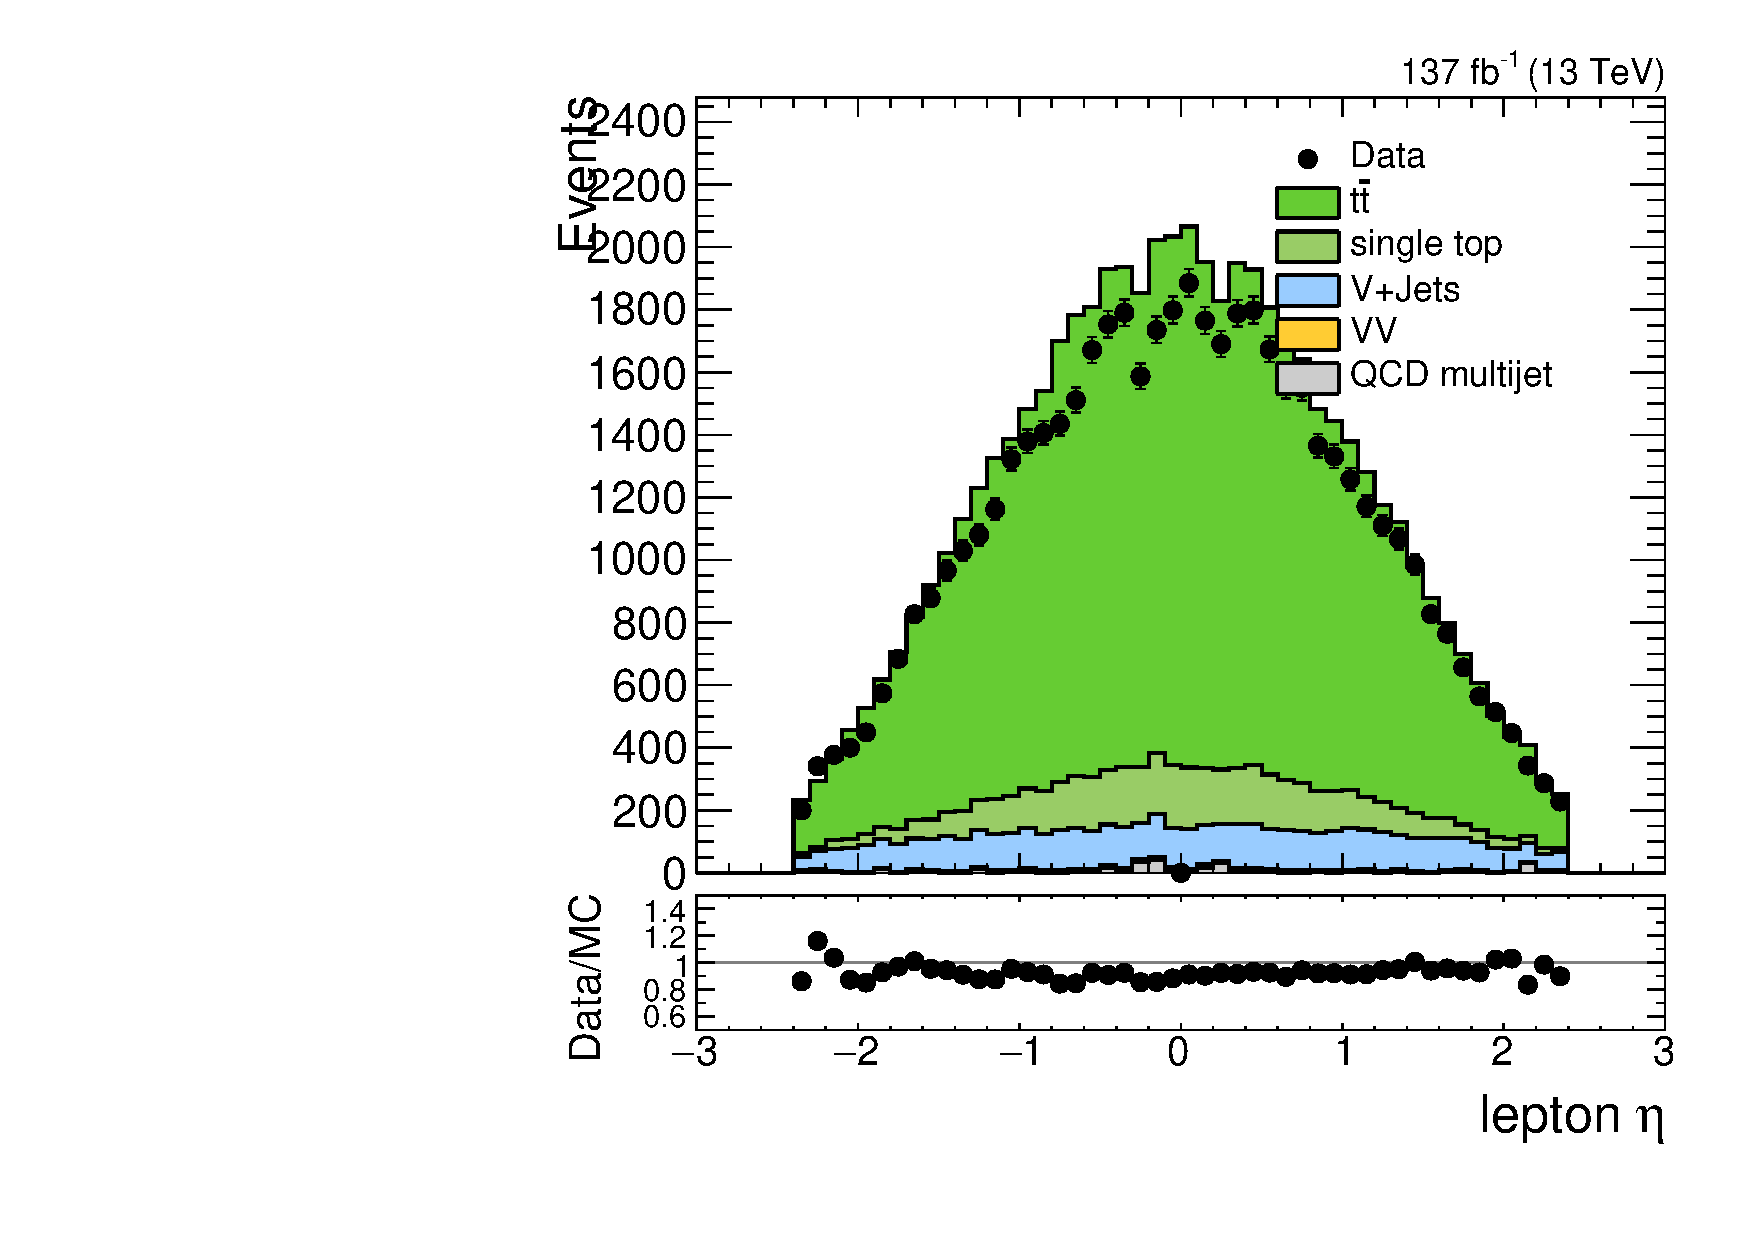
\includegraphics[width=0.3\textwidth]{fig/controlPlots/CR_b1_mu_allP_allC_allD_Run2_lnujj_l1_l_eta.pdf}
  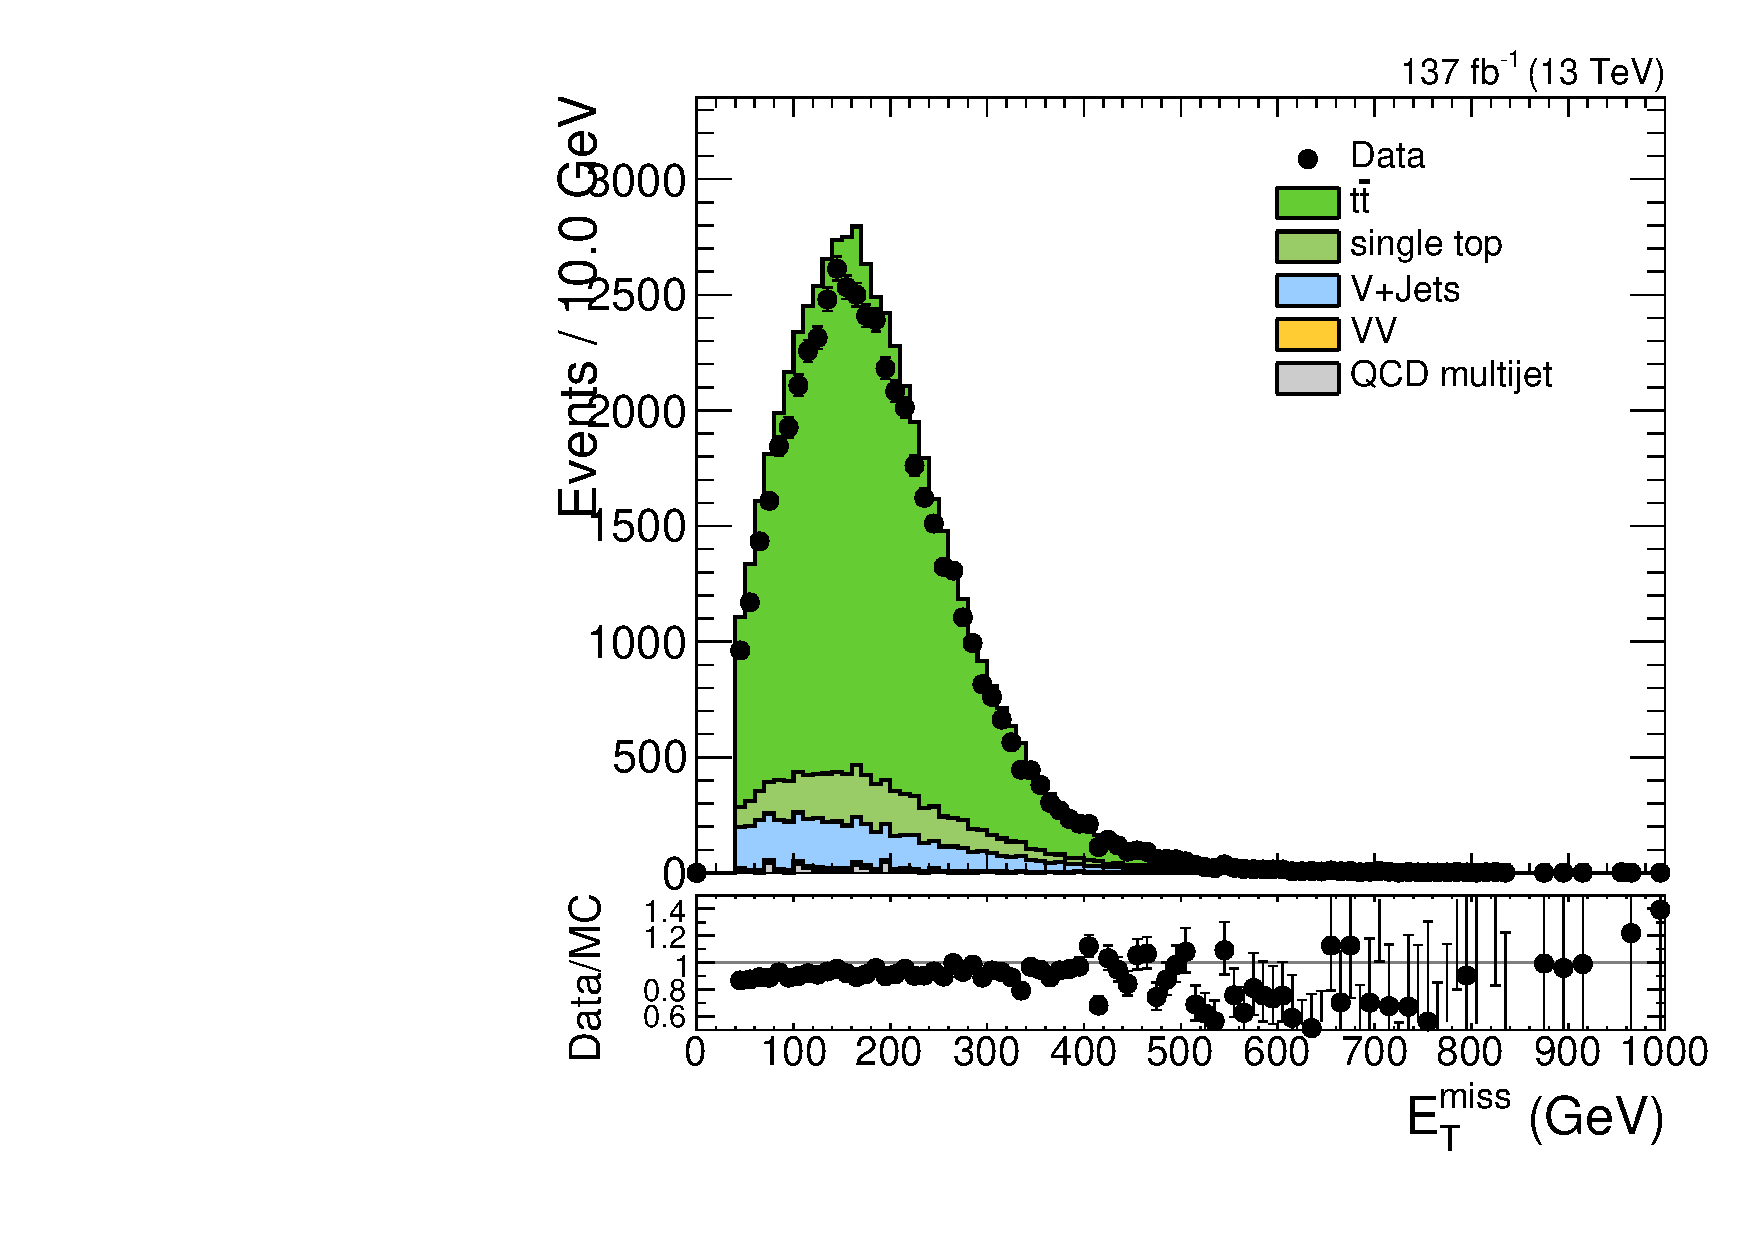
\includegraphics[width=0.3\textwidth]{fig/controlPlots/CR_b1_mu_allP_allC_allD_Run2_met_pt.pdf}\\
  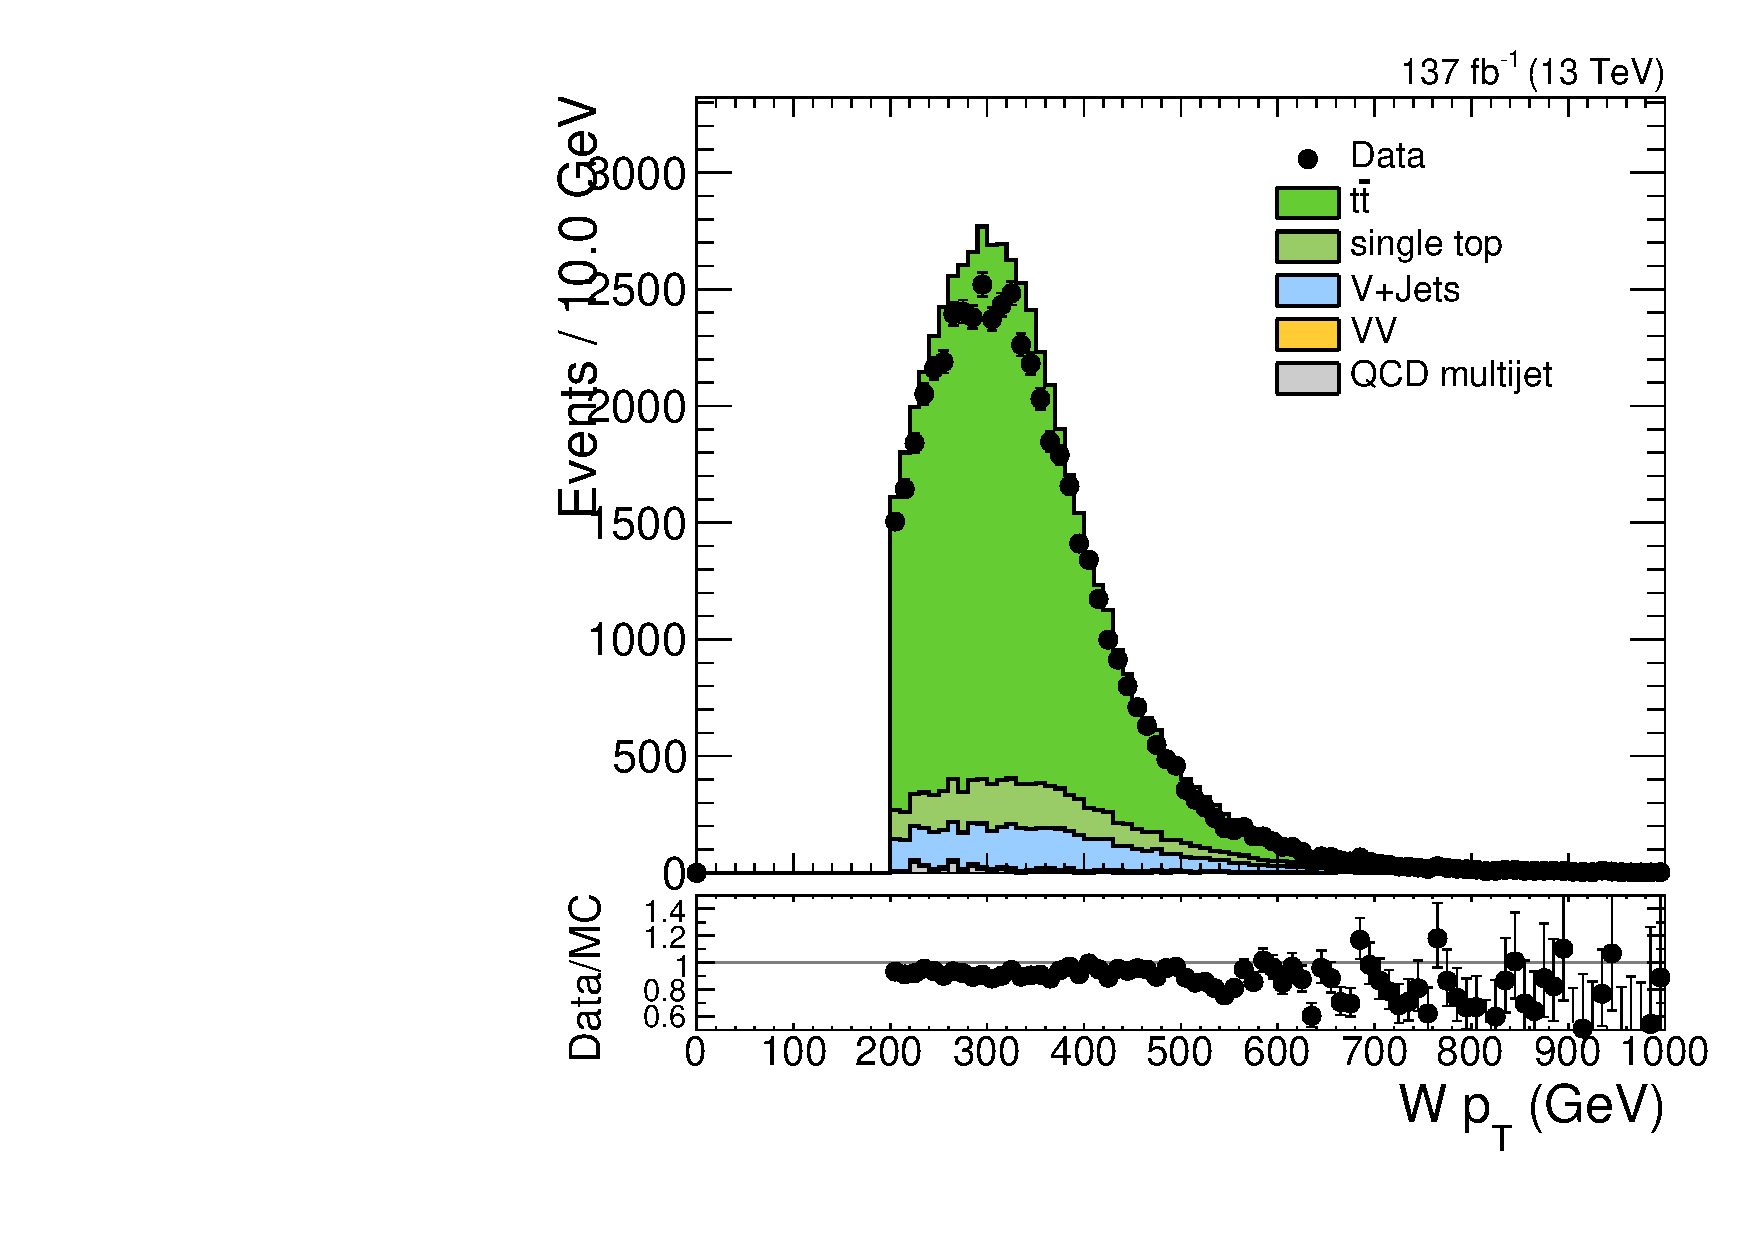
\includegraphics[width=0.3\textwidth]{fig/controlPlots/CR_b1_mu_allP_allC_allD_Run2_lnujj_l1_pt.pdf}
  \includegraphics[width=0.3\textwidth]{fig/controlPlots/CR_b1_mu_allP_allC_allD_Run2_lnujj_l1_mt.pdf}
  \includegraphics[width=0.3\textwidth]{fig/controlPlots/CR_b1_mu_allP_allC_allD_Run2_mWV.pdf}\\
  \caption{
    Comparison plots between data and MC from Run 2 for different \Wlep-related observables, in the muon channel of the top-enriched control region.
    Top row: lepton \pt, lepton $\eta$, \ptmiss.
    Bottom row: \pt of the leptonic $W^\pm$, transverse mass of the leptonic $W^\pm$, diboson invariant mass.
  }
  \label{fig:CR_controlPlotsRun2_1}
\end{figure}

\begin{figure}[htbp]
  \centering
  \includegraphics[width=0.3\textwidth]{fig/controlPlots/CR_b1_allL_allP_allC_allD_Run2_lnujj_l2_pt.pdf}
  \includegraphics[width=0.3\textwidth]{fig/controlPlots/CR_b1_allL_allP_allC_allD_Run2_lnujj_l2_eta.pdf}
  \includegraphics[width=0.3\textwidth]{fig/controlPlots/CR_b1_allL_allP_allC_allD_Run2_mjet.pdf}\\
  \includegraphics[width=0.3\textwidth]{fig/controlPlots/CR_b1_allL_allP_allC_allD_Run2_tau21DDT.pdf}
  \includegraphics[width=0.3\textwidth]{fig/controlPlots/CR_b1_allL_allP_allC_allD_Run2_DoubleB.pdf}
  \includegraphics[width=0.3\textwidth]{fig/controlPlots/CR_b1_allL_allP_allC_allD_Run2_lnujj_vbfDEta.pdf}\\
  \includegraphics[width=0.3\textwidth]{fig/controlPlots/CR_b1_allL_allP_allC_allD_Run2_lnujj_vbfMass.pdf}
  \includegraphics[width=0.3\textwidth]{fig/controlPlots/CR_b1_allL_allP_allC_allD_Run2_lnujj_nJets.pdf}
  \includegraphics[width=0.3\textwidth]{fig/controlPlots/CR_b1_allL_allP_allC_allD_Run2_dy.pdf}\\
  \caption{
    Comparison plots between data and MC from Run 2 for different \Vhad and \VBF forward jet variables, in the top-enriched control region.
    Top row: \pt, $\eta$, \MJ (soft drop mass).
    Middle row: \nsubjDDT, \DoubleB tagger of the selected \Vhad candidate, separation in $\eta$ of the \VBF forward jets.
    Bottom row: invariant mass of the \VBF jets, number of selected standard jets, rapidity separation between the reconstructed bosons.
  }
  \label{fig:CR_controlPlotsRun2_2}
\end{figure}

\clearpage
\subsection{Mitigation of Non-operational HCAL Modules in Run 2}

% Endcap issue
During Run 319077, the two HCAL towers HEM15 and HEM16 were non-operational, and the data obtained from the electron channel for the \Wtolnu candidate in those regions results in an excess of events that can be seen in figure~\ref{fig:SB_controlPlots2018_electronexcess}. % Citation
To remedy this, we exclude events recorded after Run 319077 if the lepton candidate is an electron and falls within the region $-1.55<\phi<-0.9$ and $-2.5<\eta<-1.479$.
Removing these events results in the correct behavior of the relevant kinematic variables for the electron candidate, and only discards 0.8\% of events in the signal region.

\begin{figure}[htbp]
  \centering
  \includegraphics[width=0.30\textwidth]{fig/controlPlots/SB_e_2018_lnujj_l1_l_eta.pdf}
  \includegraphics[width=0.30\textwidth]{fig/controlPlots/SB_e_2018_lnujj_l1_l_phi.pdf}
  \includegraphics[width=0.30\textwidth]{fig/controlPlots/SB_e_2018_met_phi.pdf}
  \caption{
    Comparison plots between 2018 data (including the HEM15 and HEM16 after Run 319077) and 2017 MC for the electron $\eta$, electron $\phi$, and $\phi$ of the missing transverse energy, in the jet mass sideband.
  }
  \label{fig:SB_controlPlots2018_electronexcess}
\end{figure}

% !TEX root = ../thesis.tex

\section{$V$-tagging Scale Factors}
\label{sec:vTag}

% Deriving scale factors
As mentioned previously, the top-enriched control region is obtained by inverting the $b$-tag veto, thereby requiring the presence of at least one $b$-tagged jet in the event.
The region is used to calibrate the performance of the soft drop algorithm and jet substructure variables on merged bosons.
In particular, the scale factors for the $V$-tagging selection in the HP and LP categories are derived in this region using a dedicated fit of the soft drop jet mass spectrum.
We also include events with $\nsubjDDT>0.80$ as a separate category denoted by NP to avoid bias resulting from only selecting HP and LP events.
This allows us to accurately model the $W$ peak for all categories used in the analysis.

\subsection{Fit Model}

% Fit model
Our fit model relies on two classes of events in the top-enriched region.
The first corresponds to resonant $W$ events that are the result of a top decay, with the $b$ jet outside of the AK8 jet.
The second class consists of non-resonant events resulting from random combinations of a merged AK8 jet.
To account for both of these types of events, we employ a fit model that uses a double crystal ball (DCB) for the $W$, another DCB for the partially reconstructed top quark, an exponential, and a uniform distribution.
Once the fit is performed, we then merge the second DCB, exponential, and uniform distributions to form a single non-resonant shape.

% Crystal ball function
The crystal ball function is a composite function consisting of a power-law stitched to a Gaussian core~\cite{Cheng_2016}, defined by
\begin{equation}
  f_\mathrm{CB}(x;\mu,\sigma,\alpha,n)=N
  \begin{cases}
    e^{-\frac{1}{2}\pqty{\frac{x-\mu}{\sigma}}^2}, & \frac{x-\mu}{\sigma}>-\alpha,\\
    \pqty{\frac{n}{|\alpha|}}^ne^{-\frac{|\alpha|^2}{2}}\pqty{\frac{n}{|\alpha|}-|\alpha|-\frac{x-\mu}{\sigma}}^{-n} & \frac{x-\mu}{\sigma}\leq-\alpha,
  \end{cases}
\end{equation}
where $\alpha$ is a parameter that determines the cutoff between the Gaussian core and the powertail, $n$ is the exponent of the powertail, and $N$ is a normalization factor.
The double crystal ball instead has powertails on both sides of the Gaussian core, and is given by
\begin{equation}
  f_\mathrm{DCB}(x;\mu,\sigma,\alpha_1,\alpha_2,n_1,n_2)=N
  \begin{cases}
    \pqty{\frac{n_1}{|\alpha_1|}}^{n_1}e^{-\frac{|\alpha_1|^2}{2}}\pqty{\frac{n_1}{|\alpha_1|}-|\alpha_1|-\frac{x-\mu}{\sigma}}^{-n_1} & \frac{x-\mu}{\sigma}\leq-\alpha_1,\\
    e^{-\frac{1}{2}\pqty{\frac{x-\mu}{\sigma}}^2}, & -\alpha_1<\frac{x-\mu}{\sigma}<\alpha_2,\\
    \pqty{\frac{n_2}{|\alpha_2|}}^{n_2}e^{-\frac{|\alpha_2|^2}{2}}\pqty{\frac{n_2}{|\alpha_2|}-|\alpha_2|-\frac{x-\mu}{\sigma}}^{-n_2} & \frac{x-\mu}{\sigma}\geq\alpha_2,
  \end{cases}
\end{equation}
where $\alpha_1$ and $n_1$ are the powertail parameters for the left side of the tail, and $\alpha_2$ and $n_2$ are the powertail parameters for the right side of the tail.

% Normalization
The explicit form of the fit model $f$ in each category (HP, LP, NP) is given by
\begin{align}
  & f(\mathrm{HP})=rSF^\mathrm{HP}N_W^\mathrm{HP}f_W^\mathrm{HP}+N_{NR}^\mathrm{HP}f_{NR}^\mathrm{HP},\label{eq:VtagFit1}\\
  & f(\mathrm{LP})=rSF^\mathrm{LP}N_W^\mathrm{LP}f_W^\mathrm{LP}+N_{NR}^\mathrm{LP}f_{NR}^\mathrm{LP},\label{eq:VtagFit2}\\
  & f(\mathrm{NP})=r\bqty{N_\mathrm{Total}-SF^\mathrm{HP}N_W^\mathrm{HP}-SF^\mathrm{LP}N_W^\mathrm{LP}}f_W^\mathrm{NP}+N_{NR}^\mathrm{NP}+f_{NR}^\mathrm{NP},\label{eq:VtagFit3}
\end{align}
where $f_W$ is the resonant distribution for the $W$ jet, $f_{NR}$ is the non-resonant shape, $r$ is a global scale factor accounting for lepton efficiency and luminosity, $N_{W}^\mathrm{HP}$, $N_{W}^\mathrm{LP}$, $N_{W}^\mathrm{NP}$, and $N_\mathrm{Total}$ are the number of expected events in simulation for all three categories and the total number of events, and the $SF$ are scale factors for the HP and LP categories.
This normalization is chosen to account for migration between categories.

\subsection{Fit Results}

% Fit results
We perform the fit of equations~\ref{eq:VtagFit1}-\ref{eq:VtagFit3} in a jet mass window of 20-$145\unit{GeV}$.
The resulting post-fit distributions for all three years and the full Run 2 dataset and MC samples can be seen in figure~\ref{fig:VTag_postfit_Run2}.
Table~\ref{tab:VTagFactors} shows the $V$-tagging scale factors in the HP and LP categories obtained by the fit for all years and the full Run 2 dataset, and table~\ref{tab:VScaleRes} shows the scale factors for the jet mass scale and resolution again for all years and for the full Run 2 dataset.
For the analysis we use the Run 2 scale factors in the computation of the expected signal normalizations, and the Run 2 uncertainties are used as a flat systematic uncertainty for the signal normalizations.
The scale factors for the jet mass scale and resolution are used as corrections to the signal shapes and $W$ peak for the resonant background templates.

\begin{figure}[htbp]
  \centering
  \includegraphics[width=0.3\textwidth]{fig/Vtag/PostFit__MJJ__allC_allL_HP_2016.pdf}
  \includegraphics[width=0.3\textwidth]{fig/Vtag/PostFit__MJJ__allC_allL_LP_2016.pdf}
  \includegraphics[width=0.3\textwidth]{fig/Vtag/PostFit__MJJ__allC_allL_NP_2016.pdf}\\
  \includegraphics[width=0.3\textwidth]{fig/Vtag/PostFit__MJJ__allC_allL_HP_2017.pdf}
  \includegraphics[width=0.3\textwidth]{fig/Vtag/PostFit__MJJ__allC_allL_LP_2017.pdf}
  \includegraphics[width=0.3\textwidth]{fig/Vtag/PostFit__MJJ__allC_allL_NP_2017.pdf}\\
  \includegraphics[width=0.3\textwidth]{fig/Vtag/PostFit__MJJ__allC_allL_HP_2018.pdf}
  \includegraphics[width=0.3\textwidth]{fig/Vtag/PostFit__MJJ__allC_allL_LP_2018.pdf}
  \includegraphics[width=0.3\textwidth]{fig/Vtag/PostFit__MJJ__allC_allL_NP_2018.pdf}\\
  \includegraphics[width=0.3\textwidth]{fig/Vtag/PostFit__MJJ__allC_allL_HP_Run2.pdf}
  \includegraphics[width=0.3\textwidth]{fig/Vtag/PostFit__MJJ__allC_allL_LP_Run2.pdf}
  \includegraphics[width=0.3\textwidth]{fig/Vtag/PostFit__MJJ__allC_allL_NP_Run2.pdf}\\
  \caption{
    Post-fit distributions for the background MC and dataset for all three years and Run 2 (from top to bottom: 2016, 2017, 2018, Run 2), and for the three purity categories (from left to right: HP, LP, NP).
  }
  \label{fig:VTag_postfit_Run2}
\end{figure}

\begin{table}[htbp]
  \centering
  % !TEX root = ../../thesis.tex
\footnotesize
\begin{tabular}{|ccc|}
  \hline
  Year & HP & LP \\
  \hline
  2016  & $1.02 \pm 0.04$ (stat) $\pm 0.03$ (syst) & $0.98 \pm 0.02$ (stat) $\pm 0.03$ (syst)  \\
  2017  & $0.83 \pm 0.04$ (stat) $\pm 0.03$ (syst) & $1.10 \pm 0.02$ (stat) $\pm 0.03$ (syst)  \\
  2018  & $0.87 \pm 0.03$ (stat) $\pm 0.03$ (syst) & $1.08 \pm 0.02$ (stat) $\pm 0.03$ (syst)  \\
  Run 2 & $0.88 \pm 0.02$ (stat) $\pm 0.03$ (syst) & $1.06 \pm 0.02$ (stat) $\pm 0.03$ (syst)  \\
  \hline
\end{tabular}

  \caption{
    $V$-tagging scale factors for the HP and LP categories obtained from the fit process.
  }
  \label{tab:VTagFactors}
\end{table}

\begin{table}[htbp]
  \centering
  % !TEX root = ../../thesis.tex
\footnotesize
\begin{tabular}{c|c|c}
  \hline
  Year & Scale & Resolution \\
  \hline
  \hline
  2016  & $0.991 \pm 0.003$ (stat) $\pm 0.002$ (syst) & $1.00 \pm 0.03$ (stat) $\pm 0.02$ (syst) \\
  2017  & $0.989 \pm 0.003$ (stat) $\pm 0.002$ (syst) & $1.07 \pm 0.04$ (stat) $\pm 0.02$ (syst) \\
  2018  & $0.987 \pm 0.002$ (stat) $\pm 0.002$ (syst) & $1.08 \pm 0.03$ (stat) $\pm 0.02$ (syst) \\
  Run 2 & $0.990 \pm 0.002$ (stat) $\pm 0.002$ (syst) & $1.08 \pm 0.02$ (stat) $\pm 0.02$ (syst) \\
  \hline
\end{tabular}

  \caption{
    Scale factors for the jet mass scale and resolution obtained from the fit process.
  }
  \label{tab:VScaleRes}
\end{table}

\subsection{Momentum Dependence}

% Momentum dependence
We also conduct a study on the dependence of the $V$-tagging scale factors as a function of the diboson invariant mass \MVV to apply a systematic uncertainty on the $V$-tagging process.
To do so, we measure the $V$-tagging scale factors for the full Run 2 dataset, but in three different binnings of \MVV.
We apply a low-mass binning of $[0.6,0.8\unit{TeV}]$, a mid-mass binning of $[0.8,1.0\unit{TeV}]$, and a high-mass binning of $[1.0,1.5\unit{TeV}]$.
The resulting post-fit distributions for all three binnings and for all purity categories may be see in figure~\ref{fig:VTag_postfit_massdep}.

\begin{figure}[htbp]
  \centering
  \includegraphics[width=0.3\textwidth]{fig/Vtag/PostFit__MJJ__allC_allL_HP_Low.pdf}
  \includegraphics[width=0.3\textwidth]{fig/Vtag/PostFit__MJJ__allC_allL_LP_Low.pdf}
  \includegraphics[width=0.3\textwidth]{fig/Vtag/PostFit__MJJ__allC_allL_NP_Low.pdf}\\
  \includegraphics[width=0.3\textwidth]{fig/Vtag/PostFit__MJJ__allC_allL_HP_Mid.pdf}
  \includegraphics[width=0.3\textwidth]{fig/Vtag/PostFit__MJJ__allC_allL_LP_Mid.pdf}
  \includegraphics[width=0.3\textwidth]{fig/Vtag/PostFit__MJJ__allC_allL_NP_Mid.pdf}\\
  \includegraphics[width=0.3\textwidth]{fig/Vtag/PostFit__MJJ__allC_allL_HP_High.pdf}
  \includegraphics[width=0.3\textwidth]{fig/Vtag/PostFit__MJJ__allC_allL_LP_High.pdf}
  \includegraphics[width=0.3\textwidth]{fig/Vtag/PostFit__MJJ__allC_allL_NP_High.pdf}\\
  \caption{
    Post-fit distributions for three bins of the diboson invariant mass \MVV (from top to bottom: $[0.6,0.8\unit{TeV}]$, $[0.8,1.0\unit{TeV}]$, and $[1.0,1.5\unit{TeV}]$), in the three purity categories (from left to right: HP, LP, NP), for the full Run 2 dataset.
  }
  \label{fig:VTag_postfit_massdep}
\end{figure}

% Scale factors and efficiency
The resulting scale factors, scale, and resolution as a function of \MVV are plotted in figure~\ref{fig:VTag_massdep_summary} (left).
We observe no significant dependence for $V$-tagging as a function of \MVV for the three binnings used in this study.
The $V$-tagging efficiency as a function of \MVV is also studied, which can be seen in figure~\ref{fig:VTag_massdep_summary} (right).
This allows us to place an upper limit on the uncertainty of the \pt dependence.
The fact that the scale factor is small and the simulation agrees with the data means that the scale factor will never be larger than the variations of the efficiency versus \MVV. % May need to reword
At high mass, we may therefore set an uncertainty equal to the difference of the signal efficiency at high mass versus low mass.

\begin{figure}[htbp]
  \centering
  \includegraphics[width=0.45\textwidth]{fig/Vtag/MVVDepSummary.pdf}
  \includegraphics[width=0.45\textwidth]{fig/Vtag/ptDep.pdf}
  \caption{
    Left: Plot of all scale factors as a function of the diboson invariant mass \MVV.
    Right: Plot of the $V$-tagging efficiency as a function of \MVV.
  }
  \label{fig:VTag_massdep_summary}
\end{figure}

% !TEX root = ../thesis.tex

\section{Two-dimensional Fit Process}
\label{sec:2Dfit}

% Overview of previous method
In a previous version of this analysis, the background estimation process relied upon the sideband of the groomed jet mass \MJ to estimate the background in the signal region.
This method is known as the $\alpha$ ratio method, as described by references~\cite{Khachatryan_14,Sirunyan_17}.
It involves fitting the background contributions separately on the jet mass sidebands where no signal events are expected, then using a transfer function derived in simulation to extrapolate the background in the signal region.
The transfer function $\alpha_\mathrm{MC}$ is defined by
\begin{equation}
  \alpha_\mathrm{MC}(\MVV)=\frac{F_\mathrm{MC,SR}^{\Wjets}(\MVV)}{F_\mathrm{MC,SB}^{\Wjets}(\MVV)},
\end{equation}
where $F(\MVV)$ is the probability density function used to model the \MVV spectrum in the signal and sideband regions.
For both regions, the parameterization of the background takes the form $F(x)\propto e^{c_0x+c_1/x}$.
The \Wjets background distribution in the signal region is then obtained by rescaling $F_\mathrm{Data,SB}^{\Wjets}(\MVV)$ by $\alpha_\mathrm{MC}(\MVV)$.
The resonant background contributions from \WVt are then added on top of the obtained \Wjets background in the signal region.
We then associate an uncertainty to the background prediction and select it to be large so that it covers the known differences between data and simulation, while also leaving it floating in the fitting process.
Such differences are related to modeling effects that affect the known dependence of jet mass and jet \pt, as the ungroomed jet mass $m_j$ follows the relation $\ev{m_j^2}\propto\pt^2R^2$, with jet radius $R$~\cite{shelton2013tasi}.

% Motivation for 2D method
For this analysis, we instead use a novel 2D modeling method that uses a combined fit for the resonance mass \MVV and the jet groomed mass \MJ, which captures the correlations in the fit during the likelihood minimization process.
Figure~\ref{fig:2Dfit} shows an illustration of the sideband region accessible to the 2D fit process versus the traditional jet mass sidebands used by the $\alpha$ method.
The 2D fit method allows for a simultaneous fit of the jet mass and diboson resonance sidebands due to its access to the full 2D sidebands in the \MVV-\MJ plane, whereas the $\alpha$ method is restricted to modeling background in the \MVV and \MJ spectra in separate steps.
Since the search region as defined in section~\ref{subsec:eventSelect} is the same for all signal models and accounts for the different resonances they may produce, the 2D fit also allows for treating the signal models on equal footing.

\begin{figure}[htbp]
  \centering
  % !TEX root = ../../thesis.tex
\begin{tikzpicture}
  % Jet mass sidebands
  \draw[fill=yellow!40] (0,0) rectangle (6,2) node[pos=0.5] {High jet mass sideband};
  \draw[fill=yellow!40] (0,4) rectangle (6,6) node[pos=0.5] {Low jet mass sideband};

  % Sidebands
  \draw[fill=yellow!40] (8,0) rectangle (14,6);
  \node at (11,1) {Sidebands};

  % Signal regions
  \draw[fill=red!40] (2,2) rectangle (4,4) node[pos=0.5] {Signal};
  \draw[fill=red!40] (10,2) rectangle (12,4) node[pos=0.5] {Signal};

  % Axes
  \draw[->,thick] (0,0) -- (6,0) node[below] {\MVV};
  \draw[->,thick] (0,0) -- (0,6) node[left] {\MJ};

  \draw[->,thick] (8,0) -- (14,0) node[below] {\MVV};
  \draw[->,thick] (8,0) -- (8,6) node[left] {\MJ};
\end{tikzpicture}

  \caption{
    Sideband regions of the fit for traditional sideband background estimation methods (left) versus the sideband regions in the 2D fit approach (right).
    The 2D fit method performs a simultaneous fit in the 2D sideband region in the \MVV-\MJ plane as opposed to modeling background in the \MVV and \MJ spectra in separate steps.
  }
  \label{fig:2Dfit}
\end{figure}

% Advantages of 2D fit
Thus, the 2D fit has the following advantages compared to the traditional $\alpha$ method previously used:
\begin{enumerate}
  \item The sideband as seen in figure~\ref{fig:2Dfit} is two-dimensional, thereby allowing for a simultaneous fit of the jet mass and resonance sidebands.
  This better constrains the background, which allows for better sensitivity of the search.
  \item The ability to add nuisance parameters that affect jet mass and resonance mass simultaneously, which allows us to account for the mismodeling of the correlation between the variables.
  \item Being able to use the full jet mass line-shape to extract the signal instead of using jet mass windows, providing better discrimination between $W$ and $Z$ peaks.
  \item Simultaneous fit of all \WV/\WH signals in the jet mass sideband, therefore allowing for easy implementation of exotic models such as heavy vector triplets.
\end{enumerate}

% Types of shapes in 2D fit
There are three types of shapes to consider for the 2D fit in the \MVV-\MJ plane.
The first is that of a signal process, for which we expect to see a resonance in both \MVV and \MJ.
In this case, the correlations are related to the scale and resolution of the jet.
For a background process in which there is a hadronically decaying boson (i.e., a $W$, $Z$, or $H$ from a \WVt process), we expect to observe a resonance in the \MJ dimension corresponding to the decay from the boson, but a falling spectrum in the \MVV dimension.
Lastly, if we instead have a QCD background process such as \Wjets, there will be a falling background distribution in both \MVV and \MJ, for which the shapes are correlated.

% Background types
As mentioned previously, two main classes of background are considered for this analysis, as classified based on resonant or non-resonant behavior in the \MJ spectrum:
\begin{itemize}
  \item \textbf{Resonant:} Background events in which the jet mass shape is peaking as a $W$, $Z$, $H$, or $t$ resonance in \MJ with a falling spectrum in \MVV.
  The resonant peak in \MJ is due to partially or fully merged top jets and diboson events in which one boosted boson is reconstructed into a jet.
  The main contribution is \WVt events.
  \item \textbf{Non-resonant:} Background events in which the jet is produced by the hadronization of one or more partons not originating from a vector boson.
  The dominant SM contribution is from \Wjets events, but additional contributions come from $t\bar{t}$ events as well.
\end{itemize}

% Merging samples for Run 2
The templates are derived from MC samples for both signal and background as enumerated in section~\ref{sec:samples}.
These samples were created in successive campaigns over 2016, 2017, and 2018, and are separated by their production year.
Previous versions of this analysis kept the templates separated by year, but for this iteration of the analysis we merge the samples for all three years and weight them by their respective luminosities to obtain combined Run 2 samples.
This has the benefit of providing better modeling of templates in categories with low statistics.

\subsection{Signal Modeling}
\label{sec:sig}

% Signal overview
Because the MC samples for the various signals used in the analysis only sample several points for the resonance mass \MX, we employ interpolation methods to model the signal for any arbitrary resonance mass \MX within the range 0.8-$4.5\unit{TeV}$.
To do so, we derive the each of the parameters for the signal shapes as functions of \MX, as well as the signal yield per pb of cross section as a function of \MX.

\subsubsection{Signal Shapes}

% Signal shapes
Each signal model takes the same functional form in the two-dimensional \MJ-\MVV space.
The signals are parameterized in 2D as the product of the two 1D \MJ and \MVV shapes for the jet mass and the resonance mass given by
\begin{equation}
  P_\mathrm{sig}(\MVV,\MJ|\MX)=\PVV(\MVV|\MX,\theta_1)\PJ(\MJ|\MX,\theta_2),
\end{equation}
where $\theta_1$ and $\theta_2$ are shape parameters that in principle depend on \MX.
Both shapes are modeled separately based on the jet purity (HP/LP), rapidity (HDy/LDy), and bb/nobb/vbf categories.
However, the $e$ and $\mu$ categories are merged for the signal modeling process.
To parameterize the shapes, we perform separate fits for the 1D shapes in the \MVV and \MJ spectra, then interpolate the parameters for each shape as a function of \MX to obtain $P_\mathrm{sig}(\MVV,\MJ|\MX)$ for arbitrary \MX between 1 and $4.5\unit{TeV}$.
A DCB shape is used for $\PVV(\MVV|\MX,\theta_1)$ for all categories, while the jet resonance shape $\PJ(\MJ|\MX,\theta_2)$ uses a DCB for the HP categories, and the sum of a DCB and an exponential for the LP categories.

% Signal shape parameter figures
Figures~\ref{fig:MVVShapeParam_LDy_Run2} and \ref{fig:MVVShapeParam_HDy_Run2} show the DCB parameters ($\mu$, $\sigma$, $\alpha_1$, $\alpha_2$) for the \MVV shapes in the 12 categories used to model the 2D signal shapes.
The DCB parameters for the \MJ shapes are shown in figures~\ref{fig:MJJShapeParam_LDy_Run2} and \ref{fig:MJJShapeParam_HDy_Run2}

% Signal shape substitutions
In some categories there are not enough events present that result in a smooth fit for the parameters of $\PVV(\MVV|\MX,\theta_1)$ or $\PJ(\MJ|\MX,\theta_2)$.
For example, signals that are \VBF-produced will not have a sufficient number of events present for the bb/nobb categories.
Because the signal parameters do not vary significantly between production modes, we allow for substituting non-\VBF signal shapes with \VBF shapes, and \VBF signal shapes with non-\VBF shapes:
\begin{itemize}
  \item \VBF\ZprtoWW shapes are used for \DY\ZprtoWW in the vbf categories.
  %\item \VBF\WprtoWH shapes are used for \DY\WprtoWH in the vbf categories.
  \item \VBF\WprtoWZ shapes are used for \DY\WprtoWZ in the vbf categories.
  \item \ggF\GBulktoWW shapes are used for \VBF\GBulktoWW in the bb categories.
  \item \DY\WprtoWZ shapes are used for \VBF\WprtoWZ in the bb and nobb categories.
  \item \ggF\RadtoWW shapes are used for \VBF\RadtoWW in the LP-bb categories.
  \item \ggF\GBulktoWW \MJ shapes are used for \DY\ZprtoWW \MJ in the LP-bb categories.
  \item \DY\ZprtoWW shapes are used for \VBF\ZprtoWW in the bb-LDy categories.
\end{itemize}

% Analytic signal shape figures
Figures \ref{fig:MVVShapes_NonVBF_LDy_Run2} and \ref{fig:MVVShapes_NonVBF_HDy_Run2} show the \MVV signal shapes for non-\VBF signals.
For figures \ref{fig:MVVShapes_VBF_LDy_Run2} and \ref{fig:MVVShapes_VBF_HDy_Run2}, we show the \MVV signal shapes for the \VBF signals.
In figures \ref{fig:MJJShapes_NonVBF_LDy_Run2} and \ref{fig:MJJShapes_NonVBF_HDy_Run2}, the \MJ signal shapes are shown for the non-\VBF signals.
Finally, figures \ref{fig:MJJShapes_VBF_LDy_Run2} and \ref{fig:MJJShapes_VBF_HDy_Run2} show the \MJ signal shapes for the \VBF signals.

\begin{figure}[htbp]
  \centering
  \includegraphics[width=0.2\textwidth]{fig/2Dfit/paramSignalShape_allSig_MVV_HP_bb_LDy_MEAN.pdf}
  \includegraphics[width=0.2\textwidth]{fig/2Dfit/paramSignalShape_allSig_MVV_HP_bb_LDy_SIGMA.pdf}
  \includegraphics[width=0.2\textwidth]{fig/2Dfit/paramSignalShape_allSig_MVV_HP_bb_LDy_ALPHA1.pdf}
  \includegraphics[width=0.2\textwidth]{fig/2Dfit/paramSignalShape_allSig_MVV_HP_bb_LDy_ALPHA2.pdf}\\
  \includegraphics[width=0.2\textwidth]{fig/2Dfit/paramSignalShape_allSig_MVV_LP_bb_LDy_MEAN.pdf}
  \includegraphics[width=0.2\textwidth]{fig/2Dfit/paramSignalShape_allSig_MVV_LP_bb_LDy_SIGMA.pdf}
  \includegraphics[width=0.2\textwidth]{fig/2Dfit/paramSignalShape_allSig_MVV_LP_bb_LDy_ALPHA1.pdf}
  \includegraphics[width=0.2\textwidth]{fig/2Dfit/paramSignalShape_allSig_MVV_LP_bb_LDy_ALPHA2.pdf}\\
  \includegraphics[width=0.2\textwidth]{fig/2Dfit/paramSignalShape_allSig_MVV_HP_nobb_LDy_MEAN.pdf}
  \includegraphics[width=0.2\textwidth]{fig/2Dfit/paramSignalShape_allSig_MVV_HP_nobb_LDy_SIGMA.pdf}
  \includegraphics[width=0.2\textwidth]{fig/2Dfit/paramSignalShape_allSig_MVV_HP_nobb_LDy_ALPHA1.pdf}
  \includegraphics[width=0.2\textwidth]{fig/2Dfit/paramSignalShape_allSig_MVV_HP_nobb_LDy_ALPHA2.pdf}\\
  \includegraphics[width=0.2\textwidth]{fig/2Dfit/paramSignalShape_allSig_MVV_LP_nobb_LDy_MEAN.pdf}
  \includegraphics[width=0.2\textwidth]{fig/2Dfit/paramSignalShape_allSig_MVV_LP_nobb_LDy_SIGMA.pdf}
  \includegraphics[width=0.2\textwidth]{fig/2Dfit/paramSignalShape_allSig_MVV_LP_nobb_LDy_ALPHA1.pdf}
  \includegraphics[width=0.2\textwidth]{fig/2Dfit/paramSignalShape_allSig_MVV_LP_nobb_LDy_ALPHA2.pdf}\\
  \includegraphics[width=0.2\textwidth]{fig/2Dfit/paramSignalShape_allSig_MVV_HP_vbf_LDy_MEAN.pdf}
  \includegraphics[width=0.2\textwidth]{fig/2Dfit/paramSignalShape_allSig_MVV_HP_vbf_LDy_SIGMA.pdf}
  \includegraphics[width=0.2\textwidth]{fig/2Dfit/paramSignalShape_allSig_MVV_HP_vbf_LDy_ALPHA1.pdf}
  \includegraphics[width=0.2\textwidth]{fig/2Dfit/paramSignalShape_allSig_MVV_HP_vbf_LDy_ALPHA2.pdf}\\
  \includegraphics[width=0.2\textwidth]{fig/2Dfit/paramSignalShape_allSig_MVV_LP_vbf_LDy_MEAN.pdf}
  \includegraphics[width=0.2\textwidth]{fig/2Dfit/paramSignalShape_allSig_MVV_LP_vbf_LDy_SIGMA.pdf}
  \includegraphics[width=0.2\textwidth]{fig/2Dfit/paramSignalShape_allSig_MVV_LP_vbf_LDy_ALPHA1.pdf}
  \includegraphics[width=0.2\textwidth]{fig/2Dfit/paramSignalShape_allSig_MVV_LP_vbf_LDy_ALPHA2.pdf}\\
  \caption{
    DCB parameters (from left to right: $\mu$, $\sigma$, $\alpha_1$, $\alpha_2$) for the diboson reconstructed mass \MVV as a function of \MX.
    Rows 1 to 6: HP-bb-LDy, LP-bb-LDy, HP-nobb-LDy, LP-nobb-LDy, HP-vbf-LDy, LP-vbf-LDy.
  }
  \label{fig:MVVShapeParam_LDy_Run2}
\end{figure}

\begin{figure}[htbp]
  \centering
  \includegraphics[width=0.2\textwidth]{fig/2Dfit/paramSignalShape_allSig_MVV_HP_bb_HDy_MEAN.pdf}
  \includegraphics[width=0.2\textwidth]{fig/2Dfit/paramSignalShape_allSig_MVV_HP_bb_HDy_SIGMA.pdf}
  \includegraphics[width=0.2\textwidth]{fig/2Dfit/paramSignalShape_allSig_MVV_HP_bb_HDy_ALPHA1.pdf}
  \includegraphics[width=0.2\textwidth]{fig/2Dfit/paramSignalShape_allSig_MVV_HP_bb_HDy_ALPHA2.pdf}\\
  \includegraphics[width=0.2\textwidth]{fig/2Dfit/paramSignalShape_allSig_MVV_LP_bb_HDy_MEAN.pdf}
  \includegraphics[width=0.2\textwidth]{fig/2Dfit/paramSignalShape_allSig_MVV_LP_bb_HDy_SIGMA.pdf}
  \includegraphics[width=0.2\textwidth]{fig/2Dfit/paramSignalShape_allSig_MVV_LP_bb_HDy_ALPHA1.pdf}
  \includegraphics[width=0.2\textwidth]{fig/2Dfit/paramSignalShape_allSig_MVV_LP_bb_HDy_ALPHA2.pdf}\\
  \includegraphics[width=0.2\textwidth]{fig/2Dfit/paramSignalShape_allSig_MVV_HP_nobb_HDy_MEAN.pdf}
  \includegraphics[width=0.2\textwidth]{fig/2Dfit/paramSignalShape_allSig_MVV_HP_nobb_HDy_SIGMA.pdf}
  \includegraphics[width=0.2\textwidth]{fig/2Dfit/paramSignalShape_allSig_MVV_HP_nobb_HDy_ALPHA1.pdf}
  \includegraphics[width=0.2\textwidth]{fig/2Dfit/paramSignalShape_allSig_MVV_HP_nobb_HDy_ALPHA2.pdf}\\
  \includegraphics[width=0.2\textwidth]{fig/2Dfit/paramSignalShape_allSig_MVV_LP_nobb_HDy_MEAN.pdf}
  \includegraphics[width=0.2\textwidth]{fig/2Dfit/paramSignalShape_allSig_MVV_LP_nobb_HDy_SIGMA.pdf}
  \includegraphics[width=0.2\textwidth]{fig/2Dfit/paramSignalShape_allSig_MVV_LP_nobb_HDy_ALPHA1.pdf}
  \includegraphics[width=0.2\textwidth]{fig/2Dfit/paramSignalShape_allSig_MVV_LP_nobb_HDy_ALPHA2.pdf}\\
  \includegraphics[width=0.2\textwidth]{fig/2Dfit/paramSignalShape_allSig_MVV_HP_vbf_HDy_MEAN.pdf}
  \includegraphics[width=0.2\textwidth]{fig/2Dfit/paramSignalShape_allSig_MVV_HP_vbf_HDy_SIGMA.pdf}
  \includegraphics[width=0.2\textwidth]{fig/2Dfit/paramSignalShape_allSig_MVV_HP_vbf_HDy_ALPHA1.pdf}
  \includegraphics[width=0.2\textwidth]{fig/2Dfit/paramSignalShape_allSig_MVV_HP_vbf_HDy_ALPHA2.pdf}\\
  \includegraphics[width=0.2\textwidth]{fig/2Dfit/paramSignalShape_allSig_MVV_LP_vbf_HDy_MEAN.pdf}
  \includegraphics[width=0.2\textwidth]{fig/2Dfit/paramSignalShape_allSig_MVV_LP_vbf_HDy_SIGMA.pdf}
  \includegraphics[width=0.2\textwidth]{fig/2Dfit/paramSignalShape_allSig_MVV_LP_vbf_HDy_ALPHA1.pdf}
  \includegraphics[width=0.2\textwidth]{fig/2Dfit/paramSignalShape_allSig_MVV_LP_vbf_HDy_ALPHA2.pdf}\\
  \caption{
    DCB parameters (from left to right: $\mu$, $\sigma$, $\alpha_1$, $\alpha_2$) for the diboson reconstructed mass \MVV as a function of \MX.
    Rows 1 to 6: HP-bb-HDy, LP-bb-HDy, HP-nobb-HDy, LP-nobb-HDy, HP-vbf-HDy, LP-vbf-HDy.
  }
  \label{fig:MVVShapeParam_HDy_Run2}
\end{figure}

\begin{figure}[htbp]
  \centering
  \includegraphics[width=0.2\textwidth]{fig/2Dfit/paramSignalShape_allSig_MJJ_HP_bb_LDy_mean.pdf}
  \includegraphics[width=0.2\textwidth]{fig/2Dfit/paramSignalShape_allSig_MJJ_HP_bb_LDy_sigma.pdf}
  \includegraphics[width=0.2\textwidth]{fig/2Dfit/paramSignalShape_allSig_MJJ_HP_bb_LDy_alpha.pdf}
  \includegraphics[width=0.2\textwidth]{fig/2Dfit/paramSignalShape_allSig_MJJ_HP_bb_LDy_alpha2.pdf}\\
  \includegraphics[width=0.2\textwidth]{fig/2Dfit/paramSignalShape_allSig_MJJ_LP_bb_LDy_mean.pdf}
  \includegraphics[width=0.2\textwidth]{fig/2Dfit/paramSignalShape_allSig_MJJ_LP_bb_LDy_sigma.pdf}
  \includegraphics[width=0.2\textwidth]{fig/2Dfit/paramSignalShape_allSig_MJJ_LP_bb_LDy_alpha.pdf}
  \includegraphics[width=0.2\textwidth]{fig/2Dfit/paramSignalShape_allSig_MJJ_LP_bb_LDy_alpha2.pdf}\\
  \includegraphics[width=0.2\textwidth]{fig/2Dfit/paramSignalShape_allSig_MJJ_HP_nobb_LDy_mean.pdf}
  \includegraphics[width=0.2\textwidth]{fig/2Dfit/paramSignalShape_allSig_MJJ_HP_nobb_LDy_sigma.pdf}
  \includegraphics[width=0.2\textwidth]{fig/2Dfit/paramSignalShape_allSig_MJJ_HP_nobb_LDy_alpha.pdf}
  \includegraphics[width=0.2\textwidth]{fig/2Dfit/paramSignalShape_allSig_MJJ_HP_nobb_LDy_alpha2.pdf}\\
  \includegraphics[width=0.2\textwidth]{fig/2Dfit/paramSignalShape_allSig_MJJ_LP_nobb_LDy_mean.pdf}
  \includegraphics[width=0.2\textwidth]{fig/2Dfit/paramSignalShape_allSig_MJJ_LP_nobb_LDy_sigma.pdf}
  \includegraphics[width=0.2\textwidth]{fig/2Dfit/paramSignalShape_allSig_MJJ_LP_nobb_LDy_alpha.pdf}
  \includegraphics[width=0.2\textwidth]{fig/2Dfit/paramSignalShape_allSig_MJJ_LP_nobb_LDy_alpha2.pdf}\\
  \includegraphics[width=0.2\textwidth]{fig/2Dfit/paramSignalShape_allSig_MJJ_HP_vbf_LDy_mean.pdf}
  \includegraphics[width=0.2\textwidth]{fig/2Dfit/paramSignalShape_allSig_MJJ_HP_vbf_LDy_sigma.pdf}
  \includegraphics[width=0.2\textwidth]{fig/2Dfit/paramSignalShape_allSig_MJJ_HP_vbf_LDy_alpha.pdf}
  \includegraphics[width=0.2\textwidth]{fig/2Dfit/paramSignalShape_allSig_MJJ_HP_vbf_LDy_alpha2.pdf}\\
  \includegraphics[width=0.2\textwidth]{fig/2Dfit/paramSignalShape_allSig_MJJ_LP_vbf_LDy_mean.pdf}
  \includegraphics[width=0.2\textwidth]{fig/2Dfit/paramSignalShape_allSig_MJJ_LP_vbf_LDy_sigma.pdf}
  \includegraphics[width=0.2\textwidth]{fig/2Dfit/paramSignalShape_allSig_MJJ_LP_vbf_LDy_alpha.pdf}
  \includegraphics[width=0.2\textwidth]{fig/2Dfit/paramSignalShape_allSig_MJJ_LP_vbf_LDy_alpha2.pdf}\\
  \caption{
    DCB parameters (from left to right: $\mu$, $\sigma$, $\alpha_1$, $\alpha_2$) for the jet mass \MJ as a function of \MX.
    Rows 1 to 6: HP-bb-LDy, LP-bb-LDy, HP-nobb-LDy, LP-nobb-LDy, HP-vbf-LDy, LP-vbf-LDy.
  }
  \label{fig:MJJShapeParam_LDy_Run2}
\end{figure}

\begin{figure}[htbp]
  \centering
  \includegraphics[width=0.2\textwidth]{fig/2Dfit/paramSignalShape_allSig_MJJ_HP_bb_HDy_mean.pdf}
  \includegraphics[width=0.2\textwidth]{fig/2Dfit/paramSignalShape_allSig_MJJ_HP_bb_HDy_sigma.pdf}
  \includegraphics[width=0.2\textwidth]{fig/2Dfit/paramSignalShape_allSig_MJJ_HP_bb_HDy_alpha.pdf}
  \includegraphics[width=0.2\textwidth]{fig/2Dfit/paramSignalShape_allSig_MJJ_HP_bb_HDy_alpha2.pdf}\\
  \includegraphics[width=0.2\textwidth]{fig/2Dfit/paramSignalShape_allSig_MJJ_LP_bb_HDy_mean.pdf}
  \includegraphics[width=0.2\textwidth]{fig/2Dfit/paramSignalShape_allSig_MJJ_LP_bb_HDy_sigma.pdf}
  \includegraphics[width=0.2\textwidth]{fig/2Dfit/paramSignalShape_allSig_MJJ_LP_bb_HDy_alpha.pdf}
  \includegraphics[width=0.2\textwidth]{fig/2Dfit/paramSignalShape_allSig_MJJ_LP_bb_HDy_alpha2.pdf}\\
  \includegraphics[width=0.2\textwidth]{fig/2Dfit/paramSignalShape_allSig_MJJ_HP_nobb_HDy_mean.pdf}
  \includegraphics[width=0.2\textwidth]{fig/2Dfit/paramSignalShape_allSig_MJJ_HP_nobb_HDy_sigma.pdf}
  \includegraphics[width=0.2\textwidth]{fig/2Dfit/paramSignalShape_allSig_MJJ_HP_nobb_HDy_alpha.pdf}
  \includegraphics[width=0.2\textwidth]{fig/2Dfit/paramSignalShape_allSig_MJJ_HP_nobb_HDy_alpha2.pdf}\\
  \includegraphics[width=0.2\textwidth]{fig/2Dfit/paramSignalShape_allSig_MJJ_LP_nobb_HDy_mean.pdf}
  \includegraphics[width=0.2\textwidth]{fig/2Dfit/paramSignalShape_allSig_MJJ_LP_nobb_HDy_sigma.pdf}
  \includegraphics[width=0.2\textwidth]{fig/2Dfit/paramSignalShape_allSig_MJJ_LP_nobb_HDy_alpha.pdf}
  \includegraphics[width=0.2\textwidth]{fig/2Dfit/paramSignalShape_allSig_MJJ_LP_nobb_HDy_alpha2.pdf}\\
  \includegraphics[width=0.2\textwidth]{fig/2Dfit/paramSignalShape_allSig_MJJ_HP_vbf_HDy_mean.pdf}
  \includegraphics[width=0.2\textwidth]{fig/2Dfit/paramSignalShape_allSig_MJJ_HP_vbf_HDy_sigma.pdf}
  \includegraphics[width=0.2\textwidth]{fig/2Dfit/paramSignalShape_allSig_MJJ_HP_vbf_HDy_alpha.pdf}
  \includegraphics[width=0.2\textwidth]{fig/2Dfit/paramSignalShape_allSig_MJJ_HP_vbf_HDy_alpha2.pdf}\\
  \includegraphics[width=0.2\textwidth]{fig/2Dfit/paramSignalShape_allSig_MJJ_LP_vbf_HDy_mean.pdf}
  \includegraphics[width=0.2\textwidth]{fig/2Dfit/paramSignalShape_allSig_MJJ_LP_vbf_HDy_sigma.pdf}
  \includegraphics[width=0.2\textwidth]{fig/2Dfit/paramSignalShape_allSig_MJJ_LP_vbf_HDy_alpha.pdf}
  \includegraphics[width=0.2\textwidth]{fig/2Dfit/paramSignalShape_allSig_MJJ_LP_vbf_HDy_alpha2.pdf}\\
  \caption{
    DCB parameters (from left to right: $\mu$, $\sigma$, $\alpha_1$, $\alpha_2$) for the jet mass \MJ as a function of \MX.
    Rows 1 to 6: HP-bb-HDy, LP-bb-HDy, HP-nobb-HDy, LP-nobb-HDy, HP-vbf-HDy, LP-vbf-HDy.
  }
  \label{fig:MJJShapeParam_HDy_Run2}
\end{figure}

\begin{figure}[htbp]
  \centering
  \includegraphics[width=0.18\textwidth]{fig/2Dfit/templateSignalVsMX_fromDC_GbuToWW_MVV_mu_HP_bb_LDy.pdf}
  \includegraphics[width=0.18\textwidth]{fig/2Dfit/templateSignalVsMX_fromDC_RadToWW_MVV_mu_HP_bb_LDy.pdf}
  \includegraphics[width=0.18\textwidth]{fig/2Dfit/templateSignalVsMX_fromDC_ZprToWW_MVV_mu_HP_bb_LDy.pdf}
  \includegraphics[width=0.18\textwidth]{fig/2Dfit/templateSignalVsMX_fromDC_WprToWZ_MVV_mu_HP_bb_LDy.pdf}
  \includegraphics[width=0.18\textwidth]{fig/2Dfit/templateSignalVsMX_fromDC_WprToWH_MVV_mu_HP_bb_LDy.pdf}\\
  \includegraphics[width=0.18\textwidth]{fig/2Dfit/templateSignalVsMX_fromDC_GbuToWW_MVV_mu_LP_bb_LDy.pdf}
  \includegraphics[width=0.18\textwidth]{fig/2Dfit/templateSignalVsMX_fromDC_RadToWW_MVV_mu_LP_bb_LDy.pdf}
  \includegraphics[width=0.18\textwidth]{fig/2Dfit/templateSignalVsMX_fromDC_ZprToWW_MVV_mu_LP_bb_LDy.pdf}
  \includegraphics[width=0.18\textwidth]{fig/2Dfit/templateSignalVsMX_fromDC_WprToWZ_MVV_mu_LP_bb_LDy.pdf}
  \includegraphics[width=0.18\textwidth]{fig/2Dfit/templateSignalVsMX_fromDC_WprToWH_MVV_mu_LP_bb_LDy.pdf}\\
  \includegraphics[width=0.18\textwidth]{fig/2Dfit/templateSignalVsMX_fromDC_GbuToWW_MVV_mu_HP_nobb_LDy.pdf}
  \includegraphics[width=0.18\textwidth]{fig/2Dfit/templateSignalVsMX_fromDC_RadToWW_MVV_mu_HP_nobb_LDy.pdf}
  \includegraphics[width=0.18\textwidth]{fig/2Dfit/templateSignalVsMX_fromDC_ZprToWW_MVV_mu_HP_nobb_LDy.pdf}
  \includegraphics[width=0.18\textwidth]{fig/2Dfit/templateSignalVsMX_fromDC_WprToWZ_MVV_mu_HP_nobb_LDy.pdf}
  \includegraphics[width=0.18\textwidth]{fig/2Dfit/templateSignalVsMX_fromDC_WprToWH_MVV_mu_HP_nobb_LDy.pdf}\\
  \includegraphics[width=0.18\textwidth]{fig/2Dfit/templateSignalVsMX_fromDC_GbuToWW_MVV_mu_LP_nobb_LDy.pdf}
  \includegraphics[width=0.18\textwidth]{fig/2Dfit/templateSignalVsMX_fromDC_RadToWW_MVV_mu_LP_nobb_LDy.pdf}
  \includegraphics[width=0.18\textwidth]{fig/2Dfit/templateSignalVsMX_fromDC_ZprToWW_MVV_mu_LP_nobb_LDy.pdf}
  \includegraphics[width=0.18\textwidth]{fig/2Dfit/templateSignalVsMX_fromDC_WprToWZ_MVV_mu_LP_nobb_LDy.pdf}
  \includegraphics[width=0.18\textwidth]{fig/2Dfit/templateSignalVsMX_fromDC_WprToWH_MVV_mu_LP_nobb_LDy.pdf}\\
  \includegraphics[width=0.18\textwidth]{fig/2Dfit/templateSignalVsMX_fromDC_GbuToWW_MVV_mu_HP_vbf_LDy.pdf}
  \includegraphics[width=0.18\textwidth]{fig/2Dfit/templateSignalVsMX_fromDC_RadToWW_MVV_mu_HP_vbf_LDy.pdf}
  \includegraphics[width=0.18\textwidth]{fig/2Dfit/templateSignalVsMX_fromDC_ZprToWW_MVV_mu_HP_vbf_LDy.pdf}
  \includegraphics[width=0.18\textwidth]{fig/2Dfit/templateSignalVsMX_fromDC_WprToWZ_MVV_mu_HP_vbf_LDy.pdf}
  \includegraphics[width=0.18\textwidth]{fig/2Dfit/templateSignalVsMX_fromDC_WprToWH_MVV_mu_HP_vbf_LDy.pdf}\\
  \includegraphics[width=0.18\textwidth]{fig/2Dfit/templateSignalVsMX_fromDC_GbuToWW_MVV_mu_LP_vbf_LDy.pdf}
  \includegraphics[width=0.18\textwidth]{fig/2Dfit/templateSignalVsMX_fromDC_RadToWW_MVV_mu_LP_vbf_LDy.pdf}
  \includegraphics[width=0.18\textwidth]{fig/2Dfit/templateSignalVsMX_fromDC_ZprToWW_MVV_mu_LP_vbf_LDy.pdf}
  \includegraphics[width=0.18\textwidth]{fig/2Dfit/templateSignalVsMX_fromDC_WprToWZ_MVV_mu_LP_vbf_LDy.pdf}
  \includegraphics[width=0.18\textwidth]{fig/2Dfit/templateSignalVsMX_fromDC_WprToWH_MVV_mu_LP_vbf_LDy.pdf}\\
  \caption{
    Signal shapes for the diboson reconstructed mass \MVV for \ggF- and \DY-produced signals, for 8 values of \MX.
    From left to right: \GBulktoWW, \RadtoWW, \ZprtoWW, \WprtoWZ, and \WprtoWH.
    Rows 1 to 6: HP-bb-LDy, LP-bb-LDy, HP-nobb-LDy, LP-nobb-LDy, HP-vbf-LDy, LP-vbf-LDy.
  }
  \label{fig:MVVShapes_NonVBF_LDy_Run2}
\end{figure}

\begin{figure}[htbp]
  \centering
  \includegraphics[width=0.18\textwidth]{fig/2Dfit/templateSignalVsMX_fromDC_GbuToWW_MVV_mu_HP_bb_HDy.pdf}
  \includegraphics[width=0.18\textwidth]{fig/2Dfit/templateSignalVsMX_fromDC_RadToWW_MVV_mu_HP_bb_HDy.pdf}
  \includegraphics[width=0.18\textwidth]{fig/2Dfit/templateSignalVsMX_fromDC_ZprToWW_MVV_mu_HP_bb_HDy.pdf}
  \includegraphics[width=0.18\textwidth]{fig/2Dfit/templateSignalVsMX_fromDC_WprToWZ_MVV_mu_HP_bb_HDy.pdf}
  \includegraphics[width=0.18\textwidth]{fig/2Dfit/templateSignalVsMX_fromDC_WprToWH_MVV_mu_HP_bb_HDy.pdf}\\
  \includegraphics[width=0.18\textwidth]{fig/2Dfit/templateSignalVsMX_fromDC_GbuToWW_MVV_mu_LP_bb_HDy.pdf}
  \includegraphics[width=0.18\textwidth]{fig/2Dfit/templateSignalVsMX_fromDC_RadToWW_MVV_mu_LP_bb_HDy.pdf}
  \includegraphics[width=0.18\textwidth]{fig/2Dfit/templateSignalVsMX_fromDC_ZprToWW_MVV_mu_LP_bb_HDy.pdf}
  \includegraphics[width=0.18\textwidth]{fig/2Dfit/templateSignalVsMX_fromDC_WprToWZ_MVV_mu_LP_bb_HDy.pdf}
  \includegraphics[width=0.18\textwidth]{fig/2Dfit/templateSignalVsMX_fromDC_WprToWH_MVV_mu_LP_bb_HDy.pdf}\\
  \includegraphics[width=0.18\textwidth]{fig/2Dfit/templateSignalVsMX_fromDC_GbuToWW_MVV_mu_HP_nobb_HDy.pdf}
  \includegraphics[width=0.18\textwidth]{fig/2Dfit/templateSignalVsMX_fromDC_RadToWW_MVV_mu_HP_nobb_HDy.pdf}
  \includegraphics[width=0.18\textwidth]{fig/2Dfit/templateSignalVsMX_fromDC_ZprToWW_MVV_mu_HP_nobb_HDy.pdf}
  \includegraphics[width=0.18\textwidth]{fig/2Dfit/templateSignalVsMX_fromDC_WprToWZ_MVV_mu_HP_nobb_HDy.pdf}
  \includegraphics[width=0.18\textwidth]{fig/2Dfit/templateSignalVsMX_fromDC_WprToWH_MVV_mu_HP_nobb_HDy.pdf}\\
  \includegraphics[width=0.18\textwidth]{fig/2Dfit/templateSignalVsMX_fromDC_GbuToWW_MVV_mu_LP_nobb_HDy.pdf}
  \includegraphics[width=0.18\textwidth]{fig/2Dfit/templateSignalVsMX_fromDC_RadToWW_MVV_mu_LP_nobb_HDy.pdf}
  \includegraphics[width=0.18\textwidth]{fig/2Dfit/templateSignalVsMX_fromDC_ZprToWW_MVV_mu_LP_nobb_HDy.pdf}
  \includegraphics[width=0.18\textwidth]{fig/2Dfit/templateSignalVsMX_fromDC_WprToWZ_MVV_mu_LP_nobb_HDy.pdf}
  \includegraphics[width=0.18\textwidth]{fig/2Dfit/templateSignalVsMX_fromDC_WprToWH_MVV_mu_LP_nobb_HDy.pdf}\\
  \includegraphics[width=0.18\textwidth]{fig/2Dfit/templateSignalVsMX_fromDC_GbuToWW_MVV_mu_HP_vbf_HDy.pdf}
  \includegraphics[width=0.18\textwidth]{fig/2Dfit/templateSignalVsMX_fromDC_RadToWW_MVV_mu_HP_vbf_HDy.pdf}
  \includegraphics[width=0.18\textwidth]{fig/2Dfit/templateSignalVsMX_fromDC_ZprToWW_MVV_mu_HP_vbf_HDy.pdf}
  \includegraphics[width=0.18\textwidth]{fig/2Dfit/templateSignalVsMX_fromDC_WprToWZ_MVV_mu_HP_vbf_HDy.pdf}
  \includegraphics[width=0.18\textwidth]{fig/2Dfit/templateSignalVsMX_fromDC_WprToWH_MVV_mu_HP_vbf_HDy.pdf}\\
  \includegraphics[width=0.18\textwidth]{fig/2Dfit/templateSignalVsMX_fromDC_GbuToWW_MVV_mu_LP_vbf_HDy.pdf}
  \includegraphics[width=0.18\textwidth]{fig/2Dfit/templateSignalVsMX_fromDC_RadToWW_MVV_mu_LP_vbf_HDy.pdf}
  \includegraphics[width=0.18\textwidth]{fig/2Dfit/templateSignalVsMX_fromDC_ZprToWW_MVV_mu_LP_vbf_HDy.pdf}
  \includegraphics[width=0.18\textwidth]{fig/2Dfit/templateSignalVsMX_fromDC_WprToWZ_MVV_mu_LP_vbf_HDy.pdf}
  \includegraphics[width=0.18\textwidth]{fig/2Dfit/templateSignalVsMX_fromDC_WprToWH_MVV_mu_LP_vbf_HDy.pdf}\\
  \caption{
    Signal shapes for the diboson reconstructed mass \MVV for \ggF- and \DY-produced signals, for 8 values of \MX.
    From left to right: \GBulktoWW, \RadtoWW, \ZprtoWW, \WprtoWZ, and \WprtoWH.
    Rows 1 to 6: HP-bb-HDy, LP-bb-HDy, HP-nobb-HDy, LP-nobb-HDy, HP-vbf-HDy, LP-vbf-HDy.
  }
  \label{fig:MVVShapes_NonVBF_HDy_Run2}
\end{figure}

\begin{figure}[htbp]
  \centering
  \includegraphics[width=0.18\textwidth]{fig/2Dfit/templateSignalVsMX_fromDC_VBFGbuToWW_MVV_mu_HP_bb_LDy.pdf}
  \includegraphics[width=0.18\textwidth]{fig/2Dfit/templateSignalVsMX_fromDC_VBFRadToWW_MVV_mu_HP_bb_LDy.pdf}
  \includegraphics[width=0.18\textwidth]{fig/2Dfit/templateSignalVsMX_fromDC_VBFZprToWW_MVV_mu_HP_bb_LDy.pdf}
  \includegraphics[width=0.18\textwidth]{fig/2Dfit/templateSignalVsMX_fromDC_VBFWprToWZ_MVV_mu_HP_bb_LDy.pdf}\\
  \includegraphics[width=0.18\textwidth]{fig/2Dfit/templateSignalVsMX_fromDC_VBFGbuToWW_MVV_mu_LP_bb_LDy.pdf}
  \includegraphics[width=0.18\textwidth]{fig/2Dfit/templateSignalVsMX_fromDC_VBFRadToWW_MVV_mu_LP_bb_LDy.pdf}
  \includegraphics[width=0.18\textwidth]{fig/2Dfit/templateSignalVsMX_fromDC_VBFZprToWW_MVV_mu_LP_bb_LDy.pdf}
  \includegraphics[width=0.18\textwidth]{fig/2Dfit/templateSignalVsMX_fromDC_VBFWprToWZ_MVV_mu_LP_bb_LDy.pdf}\\
  \includegraphics[width=0.18\textwidth]{fig/2Dfit/templateSignalVsMX_fromDC_VBFGbuToWW_MVV_mu_HP_nobb_LDy.pdf}
  \includegraphics[width=0.18\textwidth]{fig/2Dfit/templateSignalVsMX_fromDC_VBFRadToWW_MVV_mu_HP_nobb_LDy.pdf}
  \includegraphics[width=0.18\textwidth]{fig/2Dfit/templateSignalVsMX_fromDC_VBFZprToWW_MVV_mu_HP_nobb_LDy.pdf}
  \includegraphics[width=0.18\textwidth]{fig/2Dfit/templateSignalVsMX_fromDC_VBFWprToWZ_MVV_mu_HP_nobb_LDy.pdf}\\
  \includegraphics[width=0.18\textwidth]{fig/2Dfit/templateSignalVsMX_fromDC_VBFGbuToWW_MVV_mu_LP_nobb_LDy.pdf}
  \includegraphics[width=0.18\textwidth]{fig/2Dfit/templateSignalVsMX_fromDC_VBFRadToWW_MVV_mu_LP_nobb_LDy.pdf}
  \includegraphics[width=0.18\textwidth]{fig/2Dfit/templateSignalVsMX_fromDC_VBFZprToWW_MVV_mu_LP_nobb_LDy.pdf}
  \includegraphics[width=0.18\textwidth]{fig/2Dfit/templateSignalVsMX_fromDC_VBFWprToWZ_MVV_mu_LP_nobb_LDy.pdf}\\
  \includegraphics[width=0.18\textwidth]{fig/2Dfit/templateSignalVsMX_fromDC_VBFGbuToWW_MVV_mu_HP_vbf_LDy.pdf}
  \includegraphics[width=0.18\textwidth]{fig/2Dfit/templateSignalVsMX_fromDC_VBFRadToWW_MVV_mu_HP_vbf_LDy.pdf}
  \includegraphics[width=0.18\textwidth]{fig/2Dfit/templateSignalVsMX_fromDC_VBFZprToWW_MVV_mu_HP_vbf_LDy.pdf}
  \includegraphics[width=0.18\textwidth]{fig/2Dfit/templateSignalVsMX_fromDC_VBFWprToWZ_MVV_mu_HP_vbf_LDy.pdf}\\
  \includegraphics[width=0.18\textwidth]{fig/2Dfit/templateSignalVsMX_fromDC_VBFGbuToWW_MVV_mu_LP_vbf_LDy.pdf}
  \includegraphics[width=0.18\textwidth]{fig/2Dfit/templateSignalVsMX_fromDC_VBFRadToWW_MVV_mu_LP_vbf_LDy.pdf}
  \includegraphics[width=0.18\textwidth]{fig/2Dfit/templateSignalVsMX_fromDC_VBFZprToWW_MVV_mu_LP_vbf_LDy.pdf}
  \includegraphics[width=0.18\textwidth]{fig/2Dfit/templateSignalVsMX_fromDC_VBFWprToWZ_MVV_mu_LP_vbf_LDy.pdf}\\
  \caption{
    Signal shapes for the diboson reconstructed mass \MVV for \VBF-produced signals, for 8 values of \MX.
    From left to right: \GBulktoWW, \RadtoWW, \ZprtoWW, and \WprtoWZ.
    Rows 1 to 6: HP-bb-LDy, LP-bb-LDy, HP-nobb-LDy, LP-nobb-LDy, HP-vbf-LDy, LP-vbf-LDy.
  }
  \label{fig:MVVShapes_VBF_LDy_Run2}
\end{figure}

\begin{figure}[htbp]
  \centering
  \includegraphics[width=0.18\textwidth]{fig/2Dfit/templateSignalVsMX_fromDC_VBFGbuToWW_MVV_mu_HP_bb_HDy.pdf}
  \includegraphics[width=0.18\textwidth]{fig/2Dfit/templateSignalVsMX_fromDC_VBFRadToWW_MVV_mu_HP_bb_HDy.pdf}
  \includegraphics[width=0.18\textwidth]{fig/2Dfit/templateSignalVsMX_fromDC_VBFZprToWW_MVV_mu_HP_bb_HDy.pdf}
  \includegraphics[width=0.18\textwidth]{fig/2Dfit/templateSignalVsMX_fromDC_VBFWprToWZ_MVV_mu_HP_bb_HDy.pdf}\\
  \includegraphics[width=0.18\textwidth]{fig/2Dfit/templateSignalVsMX_fromDC_VBFGbuToWW_MVV_mu_LP_bb_HDy.pdf}
  \includegraphics[width=0.18\textwidth]{fig/2Dfit/templateSignalVsMX_fromDC_VBFRadToWW_MVV_mu_LP_bb_HDy.pdf}
  \includegraphics[width=0.18\textwidth]{fig/2Dfit/templateSignalVsMX_fromDC_VBFZprToWW_MVV_mu_LP_bb_HDy.pdf}
  \includegraphics[width=0.18\textwidth]{fig/2Dfit/templateSignalVsMX_fromDC_VBFWprToWZ_MVV_mu_LP_bb_HDy.pdf}\\
  \includegraphics[width=0.18\textwidth]{fig/2Dfit/templateSignalVsMX_fromDC_VBFGbuToWW_MVV_mu_HP_nobb_HDy.pdf}
  \includegraphics[width=0.18\textwidth]{fig/2Dfit/templateSignalVsMX_fromDC_VBFRadToWW_MVV_mu_HP_nobb_HDy.pdf}
  \includegraphics[width=0.18\textwidth]{fig/2Dfit/templateSignalVsMX_fromDC_VBFZprToWW_MVV_mu_HP_nobb_HDy.pdf}
  \includegraphics[width=0.18\textwidth]{fig/2Dfit/templateSignalVsMX_fromDC_VBFWprToWZ_MVV_mu_HP_nobb_HDy.pdf}\\
  \includegraphics[width=0.18\textwidth]{fig/2Dfit/templateSignalVsMX_fromDC_VBFGbuToWW_MVV_mu_LP_nobb_HDy.pdf}
  \includegraphics[width=0.18\textwidth]{fig/2Dfit/templateSignalVsMX_fromDC_VBFRadToWW_MVV_mu_LP_nobb_HDy.pdf}
  \includegraphics[width=0.18\textwidth]{fig/2Dfit/templateSignalVsMX_fromDC_VBFZprToWW_MVV_mu_LP_nobb_HDy.pdf}
  \includegraphics[width=0.18\textwidth]{fig/2Dfit/templateSignalVsMX_fromDC_VBFWprToWZ_MVV_mu_LP_nobb_HDy.pdf}\\
  \includegraphics[width=0.18\textwidth]{fig/2Dfit/templateSignalVsMX_fromDC_VBFGbuToWW_MVV_mu_HP_vbf_HDy.pdf}
  \includegraphics[width=0.18\textwidth]{fig/2Dfit/templateSignalVsMX_fromDC_VBFRadToWW_MVV_mu_HP_vbf_HDy.pdf}
  \includegraphics[width=0.18\textwidth]{fig/2Dfit/templateSignalVsMX_fromDC_VBFZprToWW_MVV_mu_HP_vbf_HDy.pdf}
  \includegraphics[width=0.18\textwidth]{fig/2Dfit/templateSignalVsMX_fromDC_VBFWprToWZ_MVV_mu_HP_vbf_HDy.pdf}\\
  \includegraphics[width=0.18\textwidth]{fig/2Dfit/templateSignalVsMX_fromDC_VBFGbuToWW_MVV_mu_LP_vbf_HDy.pdf}
  \includegraphics[width=0.18\textwidth]{fig/2Dfit/templateSignalVsMX_fromDC_VBFRadToWW_MVV_mu_LP_vbf_HDy.pdf}
  \includegraphics[width=0.18\textwidth]{fig/2Dfit/templateSignalVsMX_fromDC_VBFZprToWW_MVV_mu_LP_vbf_HDy.pdf}
  \includegraphics[width=0.18\textwidth]{fig/2Dfit/templateSignalVsMX_fromDC_VBFWprToWZ_MVV_mu_LP_vbf_HDy.pdf}\\
  \caption{
    Signal shapes for the diboson reconstructed mass \MVV for \VBF-produced signals, for 8 values of \MX.
    From left to right: \GBulktoWW, \RadtoWW, \ZprtoWW, and \WprtoWZ.
    Rows 1 to 6: HP-bb-HDy, LP-bb-HDy, HP-nobb-HDy, LP-nobb-HDy, HP-vbf-HDy, LP-vbf-HDy.
  }
  \label{fig:MVVShapes_VBF_HDy_Run2}
\end{figure}

\begin{figure}[htbp]
  \centering
  \includegraphics[width=0.18\textwidth]{fig/2Dfit/templateSignalVsMX_fromDC_GbuToWW_MJJ_mu_HP_bb_LDy.pdf}
  \includegraphics[width=0.18\textwidth]{fig/2Dfit/templateSignalVsMX_fromDC_RadToWW_MJJ_mu_HP_bb_LDy.pdf}
  \includegraphics[width=0.18\textwidth]{fig/2Dfit/templateSignalVsMX_fromDC_ZprToWW_MJJ_mu_HP_bb_LDy.pdf}
  \includegraphics[width=0.18\textwidth]{fig/2Dfit/templateSignalVsMX_fromDC_WprToWZ_MJJ_mu_HP_bb_LDy.pdf}
  \includegraphics[width=0.18\textwidth]{fig/2Dfit/templateSignalVsMX_fromDC_WprToWH_MJJ_mu_HP_bb_LDy.pdf}\\
  \includegraphics[width=0.18\textwidth]{fig/2Dfit/templateSignalVsMX_fromDC_GbuToWW_MJJ_mu_LP_bb_LDy.pdf}
  \includegraphics[width=0.18\textwidth]{fig/2Dfit/templateSignalVsMX_fromDC_RadToWW_MJJ_mu_LP_bb_LDy.pdf}
  \includegraphics[width=0.18\textwidth]{fig/2Dfit/templateSignalVsMX_fromDC_ZprToWW_MJJ_mu_LP_bb_LDy.pdf}
  \includegraphics[width=0.18\textwidth]{fig/2Dfit/templateSignalVsMX_fromDC_WprToWZ_MJJ_mu_LP_bb_LDy.pdf}
  \includegraphics[width=0.18\textwidth]{fig/2Dfit/templateSignalVsMX_fromDC_WprToWH_MJJ_mu_LP_bb_LDy.pdf}\\
  \includegraphics[width=0.18\textwidth]{fig/2Dfit/templateSignalVsMX_fromDC_GbuToWW_MJJ_mu_HP_nobb_LDy.pdf}
  \includegraphics[width=0.18\textwidth]{fig/2Dfit/templateSignalVsMX_fromDC_RadToWW_MJJ_mu_HP_nobb_LDy.pdf}
  \includegraphics[width=0.18\textwidth]{fig/2Dfit/templateSignalVsMX_fromDC_ZprToWW_MJJ_mu_HP_nobb_LDy.pdf}
  \includegraphics[width=0.18\textwidth]{fig/2Dfit/templateSignalVsMX_fromDC_WprToWZ_MJJ_mu_HP_nobb_LDy.pdf}
  \includegraphics[width=0.18\textwidth]{fig/2Dfit/templateSignalVsMX_fromDC_WprToWH_MJJ_mu_HP_nobb_LDy.pdf}\\
  \includegraphics[width=0.18\textwidth]{fig/2Dfit/templateSignalVsMX_fromDC_GbuToWW_MJJ_mu_LP_nobb_LDy.pdf}
  \includegraphics[width=0.18\textwidth]{fig/2Dfit/templateSignalVsMX_fromDC_RadToWW_MJJ_mu_LP_nobb_LDy.pdf}
  \includegraphics[width=0.18\textwidth]{fig/2Dfit/templateSignalVsMX_fromDC_ZprToWW_MJJ_mu_LP_nobb_LDy.pdf}
  \includegraphics[width=0.18\textwidth]{fig/2Dfit/templateSignalVsMX_fromDC_WprToWZ_MJJ_mu_LP_nobb_LDy.pdf}
  \includegraphics[width=0.18\textwidth]{fig/2Dfit/templateSignalVsMX_fromDC_WprToWH_MJJ_mu_LP_nobb_LDy.pdf}\\
  \includegraphics[width=0.18\textwidth]{fig/2Dfit/templateSignalVsMX_fromDC_GbuToWW_MJJ_mu_HP_vbf_LDy.pdf}
  \includegraphics[width=0.18\textwidth]{fig/2Dfit/templateSignalVsMX_fromDC_RadToWW_MJJ_mu_HP_vbf_LDy.pdf}
  \includegraphics[width=0.18\textwidth]{fig/2Dfit/templateSignalVsMX_fromDC_ZprToWW_MJJ_mu_HP_vbf_LDy.pdf}
  \includegraphics[width=0.18\textwidth]{fig/2Dfit/templateSignalVsMX_fromDC_WprToWZ_MJJ_mu_HP_vbf_LDy.pdf}
  \includegraphics[width=0.18\textwidth]{fig/2Dfit/templateSignalVsMX_fromDC_WprToWH_MJJ_mu_HP_vbf_LDy.pdf}\\
  \includegraphics[width=0.18\textwidth]{fig/2Dfit/templateSignalVsMX_fromDC_GbuToWW_MJJ_mu_LP_vbf_LDy.pdf}
  \includegraphics[width=0.18\textwidth]{fig/2Dfit/templateSignalVsMX_fromDC_RadToWW_MJJ_mu_LP_vbf_LDy.pdf}
  \includegraphics[width=0.18\textwidth]{fig/2Dfit/templateSignalVsMX_fromDC_ZprToWW_MJJ_mu_LP_vbf_LDy.pdf}
  \includegraphics[width=0.18\textwidth]{fig/2Dfit/templateSignalVsMX_fromDC_WprToWZ_MJJ_mu_LP_vbf_LDy.pdf}
  \includegraphics[width=0.18\textwidth]{fig/2Dfit/templateSignalVsMX_fromDC_WprToWH_MJJ_mu_LP_vbf_LDy.pdf}\\
  \caption{
    Signal shapes for the soft drop jet mass \MJ for \ggF- and \DY-produced signals, for 8 values of \MX.
    From left to right: \GBulktoWW, \RadtoWW, \ZprtoWW, \WprtoWZ, and \WprtoWH.
    Rows 1 to 6: HP-bb-LDy, LP-bb-LDy, HP-nobb-LDy, LP-nobb-LDy, HP-vbf-LDy, LP-vbf-LDy.
  }
  \label{fig:MJJShapes_NonVBF_LDy_Run2}
\end{figure}

\begin{figure}[htbp]
  \centering
  \includegraphics[width=0.18\textwidth]{fig/2Dfit/templateSignalVsMX_fromDC_GbuToWW_MJJ_mu_HP_bb_HDy.pdf}
  \includegraphics[width=0.18\textwidth]{fig/2Dfit/templateSignalVsMX_fromDC_RadToWW_MJJ_mu_HP_bb_HDy.pdf}
  \includegraphics[width=0.18\textwidth]{fig/2Dfit/templateSignalVsMX_fromDC_ZprToWW_MJJ_mu_HP_bb_HDy.pdf}
  \includegraphics[width=0.18\textwidth]{fig/2Dfit/templateSignalVsMX_fromDC_WprToWZ_MJJ_mu_HP_bb_HDy.pdf}
  \includegraphics[width=0.18\textwidth]{fig/2Dfit/templateSignalVsMX_fromDC_WprToWH_MJJ_mu_HP_bb_HDy.pdf}\\
  \includegraphics[width=0.18\textwidth]{fig/2Dfit/templateSignalVsMX_fromDC_GbuToWW_MJJ_mu_LP_bb_HDy.pdf}
  \includegraphics[width=0.18\textwidth]{fig/2Dfit/templateSignalVsMX_fromDC_RadToWW_MJJ_mu_LP_bb_HDy.pdf}
  \includegraphics[width=0.18\textwidth]{fig/2Dfit/templateSignalVsMX_fromDC_ZprToWW_MJJ_mu_LP_bb_HDy.pdf}
  \includegraphics[width=0.18\textwidth]{fig/2Dfit/templateSignalVsMX_fromDC_WprToWZ_MJJ_mu_LP_bb_HDy.pdf}
  \includegraphics[width=0.18\textwidth]{fig/2Dfit/templateSignalVsMX_fromDC_WprToWH_MJJ_mu_LP_bb_HDy.pdf}\\
  \includegraphics[width=0.18\textwidth]{fig/2Dfit/templateSignalVsMX_fromDC_GbuToWW_MJJ_mu_HP_nobb_HDy.pdf}
  \includegraphics[width=0.18\textwidth]{fig/2Dfit/templateSignalVsMX_fromDC_RadToWW_MJJ_mu_HP_nobb_HDy.pdf}
  \includegraphics[width=0.18\textwidth]{fig/2Dfit/templateSignalVsMX_fromDC_ZprToWW_MJJ_mu_HP_nobb_HDy.pdf}
  \includegraphics[width=0.18\textwidth]{fig/2Dfit/templateSignalVsMX_fromDC_WprToWZ_MJJ_mu_HP_nobb_HDy.pdf}
  \includegraphics[width=0.18\textwidth]{fig/2Dfit/templateSignalVsMX_fromDC_WprToWH_MJJ_mu_HP_nobb_HDy.pdf}\\
  \includegraphics[width=0.18\textwidth]{fig/2Dfit/templateSignalVsMX_fromDC_GbuToWW_MJJ_mu_LP_nobb_HDy.pdf}
  \includegraphics[width=0.18\textwidth]{fig/2Dfit/templateSignalVsMX_fromDC_RadToWW_MJJ_mu_LP_nobb_HDy.pdf}
  \includegraphics[width=0.18\textwidth]{fig/2Dfit/templateSignalVsMX_fromDC_ZprToWW_MJJ_mu_LP_nobb_HDy.pdf}
  \includegraphics[width=0.18\textwidth]{fig/2Dfit/templateSignalVsMX_fromDC_WprToWZ_MJJ_mu_LP_nobb_HDy.pdf}
  \includegraphics[width=0.18\textwidth]{fig/2Dfit/templateSignalVsMX_fromDC_WprToWH_MJJ_mu_LP_nobb_HDy.pdf}\\
  \includegraphics[width=0.18\textwidth]{fig/2Dfit/templateSignalVsMX_fromDC_GbuToWW_MJJ_mu_HP_vbf_HDy.pdf}
  \includegraphics[width=0.18\textwidth]{fig/2Dfit/templateSignalVsMX_fromDC_RadToWW_MJJ_mu_HP_vbf_HDy.pdf}
  \includegraphics[width=0.18\textwidth]{fig/2Dfit/templateSignalVsMX_fromDC_ZprToWW_MJJ_mu_HP_vbf_HDy.pdf}
  \includegraphics[width=0.18\textwidth]{fig/2Dfit/templateSignalVsMX_fromDC_WprToWZ_MJJ_mu_HP_vbf_HDy.pdf}
  \includegraphics[width=0.18\textwidth]{fig/2Dfit/templateSignalVsMX_fromDC_WprToWH_MJJ_mu_HP_vbf_HDy.pdf}\\
  \includegraphics[width=0.18\textwidth]{fig/2Dfit/templateSignalVsMX_fromDC_GbuToWW_MJJ_mu_LP_vbf_HDy.pdf}
  \includegraphics[width=0.18\textwidth]{fig/2Dfit/templateSignalVsMX_fromDC_RadToWW_MJJ_mu_LP_vbf_HDy.pdf}
  \includegraphics[width=0.18\textwidth]{fig/2Dfit/templateSignalVsMX_fromDC_ZprToWW_MJJ_mu_LP_vbf_HDy.pdf}
  \includegraphics[width=0.18\textwidth]{fig/2Dfit/templateSignalVsMX_fromDC_WprToWZ_MJJ_mu_LP_vbf_HDy.pdf}
  \includegraphics[width=0.18\textwidth]{fig/2Dfit/templateSignalVsMX_fromDC_WprToWH_MJJ_mu_LP_vbf_HDy.pdf}\\
  \caption{
    Signal shapes for the soft drop jet mass \MJ for \ggF- and \DY-produced signals, for 8 values of \MX.
    From left to right: \GBulktoWW, \RadtoWW, \ZprtoWW, \WprtoWZ, and \WprtoWH.
    Rows 1 to 6: HP-bb-HDy, LP-bb-HDy, HP-nobb-HDy, LP-nobb-HDy, HP-vbf-HDy, LP-vbf-HDy.
  }
  \label{fig:MJJShapes_NonVBF_HDy_Run2}
\end{figure}

\begin{figure}[htbp]
  \centering
  \includegraphics[width=0.18\textwidth]{fig/2Dfit/templateSignalVsMX_fromDC_VBFGbuToWW_MJJ_mu_HP_bb_LDy.pdf}
  \includegraphics[width=0.18\textwidth]{fig/2Dfit/templateSignalVsMX_fromDC_VBFRadToWW_MJJ_mu_HP_bb_LDy.pdf}
  \includegraphics[width=0.18\textwidth]{fig/2Dfit/templateSignalVsMX_fromDC_VBFZprToWW_MJJ_mu_HP_bb_LDy.pdf}
  \includegraphics[width=0.18\textwidth]{fig/2Dfit/templateSignalVsMX_fromDC_VBFWprToWZ_MJJ_mu_HP_bb_LDy.pdf}\\
  \includegraphics[width=0.18\textwidth]{fig/2Dfit/templateSignalVsMX_fromDC_VBFGbuToWW_MJJ_mu_LP_bb_LDy.pdf}
  \includegraphics[width=0.18\textwidth]{fig/2Dfit/templateSignalVsMX_fromDC_VBFRadToWW_MJJ_mu_LP_bb_LDy.pdf}
  \includegraphics[width=0.18\textwidth]{fig/2Dfit/templateSignalVsMX_fromDC_VBFZprToWW_MJJ_mu_LP_bb_LDy.pdf}
  \includegraphics[width=0.18\textwidth]{fig/2Dfit/templateSignalVsMX_fromDC_VBFWprToWZ_MJJ_mu_LP_bb_LDy.pdf}\\
  \includegraphics[width=0.18\textwidth]{fig/2Dfit/templateSignalVsMX_fromDC_VBFGbuToWW_MJJ_mu_HP_nobb_LDy.pdf}
  \includegraphics[width=0.18\textwidth]{fig/2Dfit/templateSignalVsMX_fromDC_VBFRadToWW_MJJ_mu_HP_nobb_LDy.pdf}
  \includegraphics[width=0.18\textwidth]{fig/2Dfit/templateSignalVsMX_fromDC_VBFZprToWW_MJJ_mu_HP_nobb_LDy.pdf}
  \includegraphics[width=0.18\textwidth]{fig/2Dfit/templateSignalVsMX_fromDC_VBFWprToWZ_MJJ_mu_HP_nobb_LDy.pdf}\\
  \includegraphics[width=0.18\textwidth]{fig/2Dfit/templateSignalVsMX_fromDC_VBFGbuToWW_MJJ_mu_LP_nobb_LDy.pdf}
  \includegraphics[width=0.18\textwidth]{fig/2Dfit/templateSignalVsMX_fromDC_VBFRadToWW_MJJ_mu_LP_nobb_LDy.pdf}
  \includegraphics[width=0.18\textwidth]{fig/2Dfit/templateSignalVsMX_fromDC_VBFZprToWW_MJJ_mu_LP_nobb_LDy.pdf}
  \includegraphics[width=0.18\textwidth]{fig/2Dfit/templateSignalVsMX_fromDC_VBFWprToWZ_MJJ_mu_LP_nobb_LDy.pdf}\\
  \includegraphics[width=0.18\textwidth]{fig/2Dfit/templateSignalVsMX_fromDC_VBFGbuToWW_MJJ_mu_HP_vbf_LDy.pdf}
  \includegraphics[width=0.18\textwidth]{fig/2Dfit/templateSignalVsMX_fromDC_VBFRadToWW_MJJ_mu_HP_vbf_LDy.pdf}
  \includegraphics[width=0.18\textwidth]{fig/2Dfit/templateSignalVsMX_fromDC_VBFZprToWW_MJJ_mu_HP_vbf_LDy.pdf}
  \includegraphics[width=0.18\textwidth]{fig/2Dfit/templateSignalVsMX_fromDC_VBFWprToWZ_MJJ_mu_HP_vbf_LDy.pdf}\\
  \includegraphics[width=0.18\textwidth]{fig/2Dfit/templateSignalVsMX_fromDC_VBFGbuToWW_MJJ_mu_LP_vbf_LDy.pdf}
  \includegraphics[width=0.18\textwidth]{fig/2Dfit/templateSignalVsMX_fromDC_VBFRadToWW_MJJ_mu_LP_vbf_LDy.pdf}
  \includegraphics[width=0.18\textwidth]{fig/2Dfit/templateSignalVsMX_fromDC_VBFZprToWW_MJJ_mu_LP_vbf_LDy.pdf}
  \includegraphics[width=0.18\textwidth]{fig/2Dfit/templateSignalVsMX_fromDC_VBFWprToWZ_MJJ_mu_LP_vbf_LDy.pdf}\\
  \caption{
    Signal shapes for the soft drop jet mass \MJ for \VBF-produced signals, for 8 values of \MX.
    From left to right: \GBulktoWW, \RadtoWW, \ZprtoWW, and \WprtoWZ.
    Rows 1 to 6: HP-bb-LDy, LP-bb-LDy, HP-nobb-LDy, LP-nobb-LDy, HP-vbf-LDy, LP-vbf-LDy.
  }
  \label{fig:MJJShapes_VBF_LDy_Run2}
\end{figure}

\begin{figure}[htbp]
  \centering
  \includegraphics[width=0.18\textwidth]{fig/2Dfit/templateSignalVsMX_fromDC_VBFGbuToWW_MJJ_mu_HP_bb_HDy.pdf}
  \includegraphics[width=0.18\textwidth]{fig/2Dfit/templateSignalVsMX_fromDC_VBFRadToWW_MJJ_mu_HP_bb_HDy.pdf}
  \includegraphics[width=0.18\textwidth]{fig/2Dfit/templateSignalVsMX_fromDC_VBFZprToWW_MJJ_mu_HP_bb_HDy.pdf}
  \includegraphics[width=0.18\textwidth]{fig/2Dfit/templateSignalVsMX_fromDC_VBFWprToWZ_MJJ_mu_HP_bb_HDy.pdf}\\
  \includegraphics[width=0.18\textwidth]{fig/2Dfit/templateSignalVsMX_fromDC_VBFGbuToWW_MJJ_mu_LP_bb_HDy.pdf}
  \includegraphics[width=0.18\textwidth]{fig/2Dfit/templateSignalVsMX_fromDC_VBFRadToWW_MJJ_mu_LP_bb_HDy.pdf}
  \includegraphics[width=0.18\textwidth]{fig/2Dfit/templateSignalVsMX_fromDC_VBFZprToWW_MJJ_mu_LP_bb_HDy.pdf}
  \includegraphics[width=0.18\textwidth]{fig/2Dfit/templateSignalVsMX_fromDC_VBFWprToWZ_MJJ_mu_LP_bb_HDy.pdf}\\
  \includegraphics[width=0.18\textwidth]{fig/2Dfit/templateSignalVsMX_fromDC_VBFGbuToWW_MJJ_mu_HP_nobb_HDy.pdf}
  \includegraphics[width=0.18\textwidth]{fig/2Dfit/templateSignalVsMX_fromDC_VBFRadToWW_MJJ_mu_HP_nobb_HDy.pdf}
  \includegraphics[width=0.18\textwidth]{fig/2Dfit/templateSignalVsMX_fromDC_VBFZprToWW_MJJ_mu_HP_nobb_HDy.pdf}
  \includegraphics[width=0.18\textwidth]{fig/2Dfit/templateSignalVsMX_fromDC_VBFWprToWZ_MJJ_mu_HP_nobb_HDy.pdf}\\
  \includegraphics[width=0.18\textwidth]{fig/2Dfit/templateSignalVsMX_fromDC_VBFGbuToWW_MJJ_mu_LP_nobb_HDy.pdf}
  \includegraphics[width=0.18\textwidth]{fig/2Dfit/templateSignalVsMX_fromDC_VBFRadToWW_MJJ_mu_LP_nobb_HDy.pdf}
  \includegraphics[width=0.18\textwidth]{fig/2Dfit/templateSignalVsMX_fromDC_VBFZprToWW_MJJ_mu_LP_nobb_HDy.pdf}
  \includegraphics[width=0.18\textwidth]{fig/2Dfit/templateSignalVsMX_fromDC_VBFWprToWZ_MJJ_mu_LP_nobb_HDy.pdf}\\
  \includegraphics[width=0.18\textwidth]{fig/2Dfit/templateSignalVsMX_fromDC_VBFGbuToWW_MJJ_mu_HP_vbf_HDy.pdf}
  \includegraphics[width=0.18\textwidth]{fig/2Dfit/templateSignalVsMX_fromDC_VBFRadToWW_MJJ_mu_HP_vbf_HDy.pdf}
  \includegraphics[width=0.18\textwidth]{fig/2Dfit/templateSignalVsMX_fromDC_VBFZprToWW_MJJ_mu_HP_vbf_HDy.pdf}
  \includegraphics[width=0.18\textwidth]{fig/2Dfit/templateSignalVsMX_fromDC_VBFWprToWZ_MJJ_mu_HP_vbf_HDy.pdf}\\
  \includegraphics[width=0.18\textwidth]{fig/2Dfit/templateSignalVsMX_fromDC_VBFGbuToWW_MJJ_mu_LP_vbf_HDy.pdf}
  \includegraphics[width=0.18\textwidth]{fig/2Dfit/templateSignalVsMX_fromDC_VBFRadToWW_MJJ_mu_LP_vbf_HDy.pdf}
  \includegraphics[width=0.18\textwidth]{fig/2Dfit/templateSignalVsMX_fromDC_VBFZprToWW_MJJ_mu_LP_vbf_HDy.pdf}
  \includegraphics[width=0.18\textwidth]{fig/2Dfit/templateSignalVsMX_fromDC_VBFWprToWZ_MJJ_mu_LP_vbf_HDy.pdf}\\
  \caption{
    Signal shapes for the soft drop jet mass \MJ for \VBF-produced signals, for 8 values of \MX.
    From left to right: \GBulktoWW, \RadtoWW, \ZprtoWW, and \WprtoWZ.
    Rows 1 to 6: HP-bb-HDy, LP-bb-HDy, HP-nobb-HDy, LP-nobb-HDy, HP-vbf-HDy, LP-vbf-HDy.
  }
  \label{fig:MJJShapes_VBF_HDy_Run2}
\end{figure}

\subsubsection{Signal Yields}

% Signal yields
The process for parameterizing the signal yield as a function of \MX is similar to obtaining the parameters for the signal shapes.
We compute the yield per pb of cross section for each mass point from our signal MC samples, then fit the result with a polynomial interpolation to obtain a function of \MX.
Figures~\ref{fig:YieldParam_NonVBF_Run2} and \ref{fig:YieldParam_VBF_Run2} show the expected yields per pb of cross section for non-\VBF and \VBF signals, respectively.

\begin{figure}[htbp]
  \centering
  \includegraphics[width=0.2\textwidth]{fig/2Dfit/paramSignalYield_NonVBFSig_mu_HP_bb_LDy.pdf}
  \includegraphics[width=0.2\textwidth]{fig/2Dfit/paramSignalYield_NonVBFSig_e_HP_bb_LDy.pdf}
  \includegraphics[width=0.2\textwidth]{fig/2Dfit/paramSignalYield_NonVBFSig_mu_LP_bb_LDy.pdf}
  \includegraphics[width=0.2\textwidth]{fig/2Dfit/paramSignalYield_NonVBFSig_e_LP_bb_LDy.pdf}\\
  \includegraphics[width=0.2\textwidth]{fig/2Dfit/paramSignalYield_NonVBFSig_mu_HP_nobb_LDy.pdf}
  \includegraphics[width=0.2\textwidth]{fig/2Dfit/paramSignalYield_NonVBFSig_e_HP_nobb_LDy.pdf}
  \includegraphics[width=0.2\textwidth]{fig/2Dfit/paramSignalYield_NonVBFSig_mu_LP_nobb_LDy.pdf}
  \includegraphics[width=0.2\textwidth]{fig/2Dfit/paramSignalYield_NonVBFSig_e_LP_nobb_LDy.pdf}\\
  \includegraphics[width=0.2\textwidth]{fig/2Dfit/paramSignalYield_NonVBFSig_mu_HP_vbf_LDy.pdf}
  \includegraphics[width=0.2\textwidth]{fig/2Dfit/paramSignalYield_NonVBFSig_e_HP_vbf_LDy.pdf}
  \includegraphics[width=0.2\textwidth]{fig/2Dfit/paramSignalYield_NonVBFSig_mu_LP_vbf_LDy.pdf}
  \includegraphics[width=0.2\textwidth]{fig/2Dfit/paramSignalYield_NonVBFSig_e_LP_vbf_LDy.pdf}\\
  \includegraphics[width=0.2\textwidth]{fig/2Dfit/paramSignalYield_NonVBFSig_mu_HP_bb_HDy.pdf}
  \includegraphics[width=0.2\textwidth]{fig/2Dfit/paramSignalYield_NonVBFSig_e_HP_bb_HDy.pdf}
  \includegraphics[width=0.2\textwidth]{fig/2Dfit/paramSignalYield_NonVBFSig_mu_LP_bb_HDy.pdf}
  \includegraphics[width=0.2\textwidth]{fig/2Dfit/paramSignalYield_NonVBFSig_e_LP_bb_HDy.pdf}\\
  \includegraphics[width=0.2\textwidth]{fig/2Dfit/paramSignalYield_NonVBFSig_mu_HP_nobb_HDy.pdf}
  \includegraphics[width=0.2\textwidth]{fig/2Dfit/paramSignalYield_NonVBFSig_e_HP_nobb_HDy.pdf}
  \includegraphics[width=0.2\textwidth]{fig/2Dfit/paramSignalYield_NonVBFSig_mu_LP_nobb_HDy.pdf}
  \includegraphics[width=0.2\textwidth]{fig/2Dfit/paramSignalYield_NonVBFSig_e_LP_nobb_HDy.pdf}\\
  \includegraphics[width=0.2\textwidth]{fig/2Dfit/paramSignalYield_NonVBFSig_mu_HP_vbf_HDy.pdf}
  \includegraphics[width=0.2\textwidth]{fig/2Dfit/paramSignalYield_NonVBFSig_e_HP_vbf_HDy.pdf}
  \includegraphics[width=0.2\textwidth]{fig/2Dfit/paramSignalYield_NonVBFSig_mu_LP_vbf_HDy.pdf}
  \includegraphics[width=0.2\textwidth]{fig/2Dfit/paramSignalYield_NonVBFSig_e_LP_vbf_HDy.pdf}\\
  \caption{
    Parameterizations of the expected yields per pb of cross section for \ggF- and \DY-produced signals as a function of \MX.
    Columns 1 to 4: $\mu$-HP, e-HP, $\mu$-LP, and e-LP.
    Rows 1 to 6: bb-LDy, nobb-LDy, vbf-LDy, bb-HDy, nobb-HDy, and vbf-HDy.}
  \label{fig:YieldParam_NonVBF_Run2}
\end{figure}

\begin{figure}[htbp]
  \centering
  \includegraphics[width=0.2\textwidth]{fig/2Dfit/paramSignalYield_VBFSig_mu_HP_bb_LDy.pdf}
  \includegraphics[width=0.2\textwidth]{fig/2Dfit/paramSignalYield_VBFSig_e_HP_bb_LDy.pdf}
  \includegraphics[width=0.2\textwidth]{fig/2Dfit/paramSignalYield_VBFSig_mu_LP_bb_LDy.pdf}
  \includegraphics[width=0.2\textwidth]{fig/2Dfit/paramSignalYield_VBFSig_e_LP_bb_LDy.pdf}\\
  \includegraphics[width=0.2\textwidth]{fig/2Dfit/paramSignalYield_VBFSig_mu_HP_nobb_LDy.pdf}
  \includegraphics[width=0.2\textwidth]{fig/2Dfit/paramSignalYield_VBFSig_e_HP_nobb_LDy.pdf}
  \includegraphics[width=0.2\textwidth]{fig/2Dfit/paramSignalYield_VBFSig_mu_LP_nobb_LDy.pdf}
  \includegraphics[width=0.2\textwidth]{fig/2Dfit/paramSignalYield_VBFSig_e_LP_nobb_LDy.pdf}\\
  \includegraphics[width=0.2\textwidth]{fig/2Dfit/paramSignalYield_VBFSig_mu_HP_vbf_LDy.pdf}
  \includegraphics[width=0.2\textwidth]{fig/2Dfit/paramSignalYield_VBFSig_e_HP_vbf_LDy.pdf}
  \includegraphics[width=0.2\textwidth]{fig/2Dfit/paramSignalYield_VBFSig_mu_LP_vbf_LDy.pdf}
  \includegraphics[width=0.2\textwidth]{fig/2Dfit/paramSignalYield_VBFSig_e_LP_vbf_LDy.pdf}\\
  \includegraphics[width=0.2\textwidth]{fig/2Dfit/paramSignalYield_VBFSig_mu_HP_bb_HDy.pdf}
  \includegraphics[width=0.2\textwidth]{fig/2Dfit/paramSignalYield_VBFSig_e_HP_bb_HDy.pdf}
  \includegraphics[width=0.2\textwidth]{fig/2Dfit/paramSignalYield_VBFSig_mu_LP_bb_HDy.pdf}
  \includegraphics[width=0.2\textwidth]{fig/2Dfit/paramSignalYield_VBFSig_e_LP_bb_HDy.pdf}\\
  \includegraphics[width=0.2\textwidth]{fig/2Dfit/paramSignalYield_VBFSig_mu_HP_nobb_HDy.pdf}
  \includegraphics[width=0.2\textwidth]{fig/2Dfit/paramSignalYield_VBFSig_e_HP_nobb_HDy.pdf}
  \includegraphics[width=0.2\textwidth]{fig/2Dfit/paramSignalYield_VBFSig_mu_LP_nobb_HDy.pdf}
  \includegraphics[width=0.2\textwidth]{fig/2Dfit/paramSignalYield_VBFSig_e_LP_nobb_HDy.pdf}\\
  \includegraphics[width=0.2\textwidth]{fig/2Dfit/paramSignalYield_VBFSig_mu_HP_vbf_HDy.pdf}
  \includegraphics[width=0.2\textwidth]{fig/2Dfit/paramSignalYield_VBFSig_e_HP_vbf_HDy.pdf}
  \includegraphics[width=0.2\textwidth]{fig/2Dfit/paramSignalYield_VBFSig_mu_LP_vbf_HDy.pdf}
  \includegraphics[width=0.2\textwidth]{fig/2Dfit/paramSignalYield_VBFSig_e_LP_vbf_HDy.pdf}\\
  \caption{
    Parameterizations of the expected yields per pb of cross section for \VBF-produced signals as a function of \MX.
    Columns 1 to 4: $\mu$-HP, e-HP, $\mu$-LP, and e-LP.
    Rows 1 to 6: bb-LDy, nobb-LDy, vbf-LDy, bb-HDy, nobb-HDy, and vbf-HDy.}
  \label{fig:YieldParam_VBF_Run2}
\end{figure}

\subsection{Background Modeling}
\label{sec:bkg}

% Background template overview
Unlike the signal shapes described in the previous section, both the resonant and non-resonant background modeling involve 2D histograms rather than smooth shapes.
This is in part due to the challenges encountered with the modeling process, which is a result of the low statistics for the background MC samples after applying the selection cuts.

\subsubsection{Non-resonant Background Templates}

% Non-resonant background templates overview
The non-resonant background templates are modeled with conditional products, taking the form
\begin{equation}
  P_{\Wjets}(\MVV,\MJ)=\PVV(\MVV|\MJ,\theta_1)\PJ(\MJ|\theta_2).
\end{equation}
For $\PJ(\MJ|\theta_2)$ we derive a 1D template for the \MJ distribution, which we then multiply with a 2D shape from $\PVV(\MVV|\MJ,\theta_1)$ for the \MVV distribution.

% 2D conditional template
For the 2D \MVV shape, we use a specialized Gaussian kernel method in order overcome the low statistics encountered for the background MC events.
Standard Gaussian methods were found to be ineffective at capturing peaks in the 2D plane, as they would result in a smearing of the peaks from reconstructed simulation events.
To remedy this, we employ a method in which we use a partially generated diboson invariant mass \MVVpart, which is defined as the four vector sum of the reconstructed \Wlep, and a generated jet.
The generated jet is made by clustering generated particle candidates with $\Delta R<1.2$ around reconstructed jets using the anti-\kt algorithm with a distance parameter of $R=0.8$.

% Response function
Because the generated jets are used in place of the reconstructed \Vhad, we must make use of a detector response function to accurately model reconstruction of the simulated jets.
This is done in simulation by estimating the Gaussian mean and sigma of the resolution of $\MVV/\MVVpart$ in bins of generator jet \pt, which can be seen in figure~\ref{fig:nonResScaleResMVV}.
We then begin generating the template by populating the \MJ spectrum using a coarse binning.
For each event in a slice of the \MJ spectrum, we add a 1D Gaussian onto the partial mass with scale shifted by the detector response and width equal to the Gaussian resolution as defined by
\begin{equation}\label{eq:Pplus}
  P_+=\frac{w_i}{\sqrt{2\pi}\sigma}\exp\bqty{-\frac{1}{2}\pqty{\frac{x-s\MVVpart}{\sigma}}^2},
\end{equation}
where $w_i$ is the event weight, and $s$ and $\sigma$ are the scale and resolution parameters obtained from the detector response.

\begin{figure}[htbp]
  \centering
  \includegraphics[width=0.4\textwidth]{fig/2Dfit/detectorParam_nonRes_scale_MVV.pdf}
  \includegraphics[width=0.4\textwidth]{fig/2Dfit/detectorParam_nonRes_resolution_MVV.pdf}
  \caption{
    Scale (left) and resolution (right) of \MVV as a function of the generated jet \pt.
  }
  \label{fig:nonResScaleResMVV}
\end{figure}

% Template smoothing
Another issue encountered with the low statistics of the MC samples is the lack of events at higher values of \MVV.
To address this, we perform a smoothing of the tails of the \MVV shape with a power law function in each bin of \MJ.
We then populate the 2D histogram with values from the \MVV shape in each \MJ bin, with the power law functions sampled from $1.2\unit{TeV}$ and onward for the bb categories, and $1.6\unit{TeV}$ and onward for the nobb categories.

% Template conditionality
To ensure that the template is conditional with respect to \MJ, each histogram slice corresponding to one crude bin of \MJ is normalized.
We then interpolate over the coarsely binned \MJ histogram for each \MVV bin using a spline, which is used to populate the 2D histogram.
As a final step, we normalize each \MJ slice again to ensure the conditionality of the template.

% Merged categories
Ideally, this process of generating the 2D conditional templates would be done for all 24 categories as defined in subsection~\ref{subsec:eventCat}.
However, this is met with more difficulties due to the low statistics provided by the MC samples.
To resolve this issue, we merge categories together based on whether or not they exhibit similar behavior.
We consider various metrics of behavior between categories, such as the correlation between \MJ and \MVV, as well as the average jet \pt as a function of the jet mass, which is shown in figure~\ref{fig:nonRes2DCorr} between the four combinations of HP/LP and nobb/bb categories.
The behavior is similar enough between the categories that they may be considered for merging.
For this analysis, we merge the $e$/$\mu$ and bb/nobb/vbf categories while keeping the HP/LP and HDy/LDy categories separate, for a total of four 2D conditional templates.

\begin{figure}[htbp]
  \centering
  \includegraphics[width=0.45\textwidth]{fig/2Dfit/nonRes_corr.pdf}
  \caption{
    Average \pt of the jet as a function of the jet mass \MJ compared between the four combinations of HP/LP and nobb/bb categories for the non-resonant background MC samples.
  }
  \label{fig:nonRes2DCorr}
\end{figure}

% Reweighting templates
Prior to creating the 2D conditional templates, a reweighting procedure is applied in the jet mass sideband region for the \MVV spectrum in order to ensure that the templates accurately capture the behavior of the background events.
We again merge the $e$ and $\mu$ categories for this process due to their similar behavior, but for other categories such as nobb/bb/vbf, we derive separate weighting functions for the \MVV spectrum.
The categories are then merged to create the four conditional 2D templates after the weighting process.
The reweighting function takes the form $f(\MVV)=a+b/\MVV$ to ensure that the weights behave as expected in the asymptotic limit, and the fit coefficients are derived by fitting the function to the ratio of data to MC.
From this we obtain the weights $w_i$ of equation~\ref{eq:Pplus}.
Figure~\ref{fig:nonResMvvSpectrumReweighting} shows the \MVV distributions from which the weights are derived.

\begin{figure}[htbp]
  \centering
  \includegraphics[width=0.2\textwidth]{fig/2Dfit/slopesSB_b1_allL_HP_bb_LDy_Run2_mWV_1OverX.pdf}
  \includegraphics[width=0.2\textwidth]{fig/2Dfit/slopesSB_b1_allL_LP_bb_LDy_Run2_mWV_1OverX.pdf}
  \includegraphics[width=0.2\textwidth]{fig/2Dfit/slopesSB_b1_allL_HP_bb_HDy_Run2_mWV_1OverX.pdf}
  \includegraphics[width=0.2\textwidth]{fig/2Dfit/slopesSB_b1_allL_LP_bb_HDy_Run2_mWV_1OverX.pdf}\\
  \includegraphics[width=0.2\textwidth]{fig/2Dfit/slopesSB_b1_allL_HP_nobb_LDy_Run2_mWV_1OverX.pdf}
  \includegraphics[width=0.2\textwidth]{fig/2Dfit/slopesSB_b1_allL_LP_nobb_LDy_Run2_mWV_1OverX.pdf}
  \includegraphics[width=0.2\textwidth]{fig/2Dfit/slopesSB_b1_allL_HP_nobb_HDy_Run2_mWV_1OverX.pdf}
  \includegraphics[width=0.2\textwidth]{fig/2Dfit/slopesSB_b1_allL_LP_nobb_HDy_Run2_mWV_1OverX.pdf}\\
  \includegraphics[width=0.2\textwidth]{fig/2Dfit/slopesSB_b1_allL_HP_vbf_LDy_Run2_mWV_1OverX.pdf}
  \includegraphics[width=0.2\textwidth]{fig/2Dfit/slopesSB_b1_allL_LP_vbf_LDy_Run2_mWV_1OverX.pdf}
  \includegraphics[width=0.2\textwidth]{fig/2Dfit/slopesSB_b1_allL_HP_vbf_HDy_Run2_mWV_1OverX.pdf}
  \includegraphics[width=0.2\textwidth]{fig/2Dfit/slopesSB_b1_allL_LP_vbf_HDy_Run2_mWV_1OverX.pdf}\\
  \caption{
    Plots of the \MVV spectra for the full Run 2 data and MC samples in the jet mass sideband for each category, with the $e$ and $\mu$ categories merged.
    After merging the $e$ and $\mu$ categories, the remaining categories are kept separate and the ratio of data to MC is fitted with a function of the form $f(\MVV)=a+b/\MVV$.
    The resulting weights for each event $w_i$ are then used in equation~\ref{eq:Pplus} when building the conditional 2D templates.
    Columns 1 to 4: HP-LDy, LP-LDy, HP-HDy, and LP-HDy.
    Rows 1 to 3: bb, nobb, and vbf for data, but with merged bb+nobb+vbf distributions for the MC.
  }
  \label{fig:nonResMvvSpectrumReweighting}
\end{figure}

% Non-resonant closure test
As a check on the closure of the 2D conditional template building process, we plot the projection of the templates on the \MVV spectrum versus the weighted MC distributions.
Figure~\ref{fig:condTemplateVscondReco_nonRes_MVV_Run2} shows the resulting comparison between the templates and the MC samples for each of the four merged categories, which show good agreement between each other.

\begin{figure}[htbp]
  \centering
  \includegraphics[width=0.45\textwidth]{fig/2Dfit/templateVsReco_nonResCond_MVV_e_HP_nobb_LDy.pdf}
  \includegraphics[width=0.45\textwidth]{fig/2Dfit/templateVsReco_nonResCond_MVV_e_HP_nobb_HDy.pdf}\\
  \includegraphics[width=0.45\textwidth]{fig/2Dfit/templateVsReco_nonResCond_MVV_e_LP_nobb_LDy.pdf}
  \includegraphics[width=0.45\textwidth]{fig/2Dfit/templateVsReco_nonResCond_MVV_e_LP_nobb_HDy.pdf}\\
  \caption{
    Projection onto the \MVV spectrum of the 2D conditional non-resonant background templates (solid lines) versus the weighted MC distributions (points) used to make them, for the HP-LDy (top left), HP-HDy (top right), LP-LDy (bottom left), and LP-HDy (bottom right) merged categories.
    Four separate \MJ ranges are plotted, with one corresponding to the full \MJ range, and three corresponding to the sub-ranges.
  }
  \label{fig:condTemplateVscondReco_nonRes_MVV_Run2}
\end{figure}

% 1D non-resonant soft drop jet mass templates
The remaining step to complete the conditional product $P_{\Wjets}(\MVV,\MJ)$ is to obtain the 1D template for $\PJ(\MJ|\theta_2)$.
Rather than using a kernel method as with the 2D conditional template, we instead use a coarsely binned histogram of weighted MC events for \MJ, and then fit the result with a spline.
The spline is then used to interpolate the $\PJ(\MJ|\theta_2)$ template with the final \MJ binning.
In this case, we also do not merge any of the 24 categories and keep the templates separate.
Figure~\ref{fig:1dtemplateVsReco_nonRes_MJ_Run2} shows the resulting 1D templates for each category compared to the weighted MC distributions used to obtain them.

\begin{figure}[htbp]
  \centering
  \includegraphics[width=0.2\textwidth]{fig/2Dfit/templateVsReco_nonRes_r0_MJ_mu_HP_bb_LDy.pdf}
  \includegraphics[width=0.2\textwidth]{fig/2Dfit/templateVsReco_nonRes_r0_MJ_e_HP_bb_LDy.pdf}
  \includegraphics[width=0.2\textwidth]{fig/2Dfit/templateVsReco_nonRes_r0_MJ_mu_LP_bb_LDy.pdf}
  \includegraphics[width=0.2\textwidth]{fig/2Dfit/templateVsReco_nonRes_r0_MJ_e_LP_bb_LDy.pdf}\\
  \includegraphics[width=0.2\textwidth]{fig/2Dfit/templateVsReco_nonRes_r0_MJ_mu_HP_nobb_LDy.pdf}
  \includegraphics[width=0.2\textwidth]{fig/2Dfit/templateVsReco_nonRes_r0_MJ_e_HP_nobb_LDy.pdf}
  \includegraphics[width=0.2\textwidth]{fig/2Dfit/templateVsReco_nonRes_r0_MJ_mu_LP_nobb_LDy.pdf}
  \includegraphics[width=0.2\textwidth]{fig/2Dfit/templateVsReco_nonRes_r0_MJ_e_LP_nobb_LDy.pdf}\\
  \includegraphics[width=0.2\textwidth]{fig/2Dfit/templateVsReco_nonRes_r0_MJ_mu_HP_vbf_LDy.pdf}
  \includegraphics[width=0.2\textwidth]{fig/2Dfit/templateVsReco_nonRes_r0_MJ_e_HP_vbf_LDy.pdf}
  \includegraphics[width=0.2\textwidth]{fig/2Dfit/templateVsReco_nonRes_r0_MJ_mu_LP_vbf_LDy.pdf}
  \includegraphics[width=0.2\textwidth]{fig/2Dfit/templateVsReco_nonRes_r0_MJ_e_LP_vbf_LDy.pdf}\\
  \includegraphics[width=0.2\textwidth]{fig/2Dfit/templateVsReco_nonRes_r0_MJ_mu_HP_bb_HDy.pdf}
  \includegraphics[width=0.2\textwidth]{fig/2Dfit/templateVsReco_nonRes_r0_MJ_e_HP_bb_HDy.pdf}
  \includegraphics[width=0.2\textwidth]{fig/2Dfit/templateVsReco_nonRes_r0_MJ_mu_LP_bb_HDy.pdf}
  \includegraphics[width=0.2\textwidth]{fig/2Dfit/templateVsReco_nonRes_r0_MJ_e_LP_bb_HDy.pdf}\\
  \includegraphics[width=0.2\textwidth]{fig/2Dfit/templateVsReco_nonRes_r0_MJ_mu_HP_nobb_HDy.pdf}
  \includegraphics[width=0.2\textwidth]{fig/2Dfit/templateVsReco_nonRes_r0_MJ_e_HP_nobb_HDy.pdf}
  \includegraphics[width=0.2\textwidth]{fig/2Dfit/templateVsReco_nonRes_r0_MJ_mu_LP_nobb_HDy.pdf}
  \includegraphics[width=0.2\textwidth]{fig/2Dfit/templateVsReco_nonRes_r0_MJ_e_LP_nobb_HDy.pdf}\\
  \includegraphics[width=0.2\textwidth]{fig/2Dfit/templateVsReco_nonRes_r0_MJ_mu_HP_vbf_HDy.pdf}
  \includegraphics[width=0.2\textwidth]{fig/2Dfit/templateVsReco_nonRes_r0_MJ_e_HP_vbf_HDy.pdf}
  \includegraphics[width=0.2\textwidth]{fig/2Dfit/templateVsReco_nonRes_r0_MJ_mu_LP_vbf_HDy.pdf}
  \includegraphics[width=0.2\textwidth]{fig/2Dfit/templateVsReco_nonRes_r0_MJ_e_LP_vbf_HDy.pdf}\\
  \caption{
    Comparison of the 1D \MJ templates for the non-resonant background (solid line) and the weighted MC distributions (points).
    Columns 1 to 4: $\mu$-HP, $e$-HP, $\mu$-LP, and $e$-LP.
    Rows 1 to 6: bb-LDy, nobb-LDy, vbf-LDy, bb-HDy, nobb-HDy, and vbf-HDy.
  }
  \label{fig:1dtemplateVsReco_nonRes_MJ_Run2}
\end{figure}

% Final non-resonant templates
The final non-resonant templates are then obtained from the product of the 2D conditional template with the 1D jet mass shape.
Figure~\ref{fig:templates_nonRes_Run2} shows the 2D templates for each of the 24 categories.
To better visualize the differences between each of the categories, figure~\ref{fig:compTemplate_nonRes} shows comparisons of the \MVV and \MJ projections of the templates for each category.

\begin{figure}[htbp]
  \centering
  \includegraphics[width=0.2\textwidth]{fig/2Dfit/template_nonRes_mu_HP_bb_LDy.pdf}
  \includegraphics[width=0.2\textwidth]{fig/2Dfit/template_nonRes_e_HP_bb_LDy.pdf}
  \includegraphics[width=0.2\textwidth]{fig/2Dfit/template_nonRes_mu_LP_bb_LDy.pdf}
  \includegraphics[width=0.2\textwidth]{fig/2Dfit/template_nonRes_e_LP_bb_LDy.pdf}\\
  \includegraphics[width=0.2\textwidth]{fig/2Dfit/template_nonRes_mu_HP_nobb_LDy.pdf}
  \includegraphics[width=0.2\textwidth]{fig/2Dfit/template_nonRes_e_HP_nobb_LDy.pdf}
  \includegraphics[width=0.2\textwidth]{fig/2Dfit/template_nonRes_mu_LP_nobb_LDy.pdf}
  \includegraphics[width=0.2\textwidth]{fig/2Dfit/template_nonRes_e_LP_nobb_LDy.pdf}\\
  \includegraphics[width=0.2\textwidth]{fig/2Dfit/template_nonRes_mu_HP_vbf_LDy.pdf}
  \includegraphics[width=0.2\textwidth]{fig/2Dfit/template_nonRes_e_HP_vbf_LDy.pdf}
  \includegraphics[width=0.2\textwidth]{fig/2Dfit/template_nonRes_mu_LP_vbf_LDy.pdf}
  \includegraphics[width=0.2\textwidth]{fig/2Dfit/template_nonRes_e_LP_vbf_LDy.pdf}\\
  \includegraphics[width=0.2\textwidth]{fig/2Dfit/template_nonRes_mu_HP_bb_HDy.pdf}
  \includegraphics[width=0.2\textwidth]{fig/2Dfit/template_nonRes_e_HP_bb_HDy.pdf}
  \includegraphics[width=0.2\textwidth]{fig/2Dfit/template_nonRes_mu_LP_bb_HDy.pdf}
  \includegraphics[width=0.2\textwidth]{fig/2Dfit/template_nonRes_e_LP_bb_HDy.pdf}\\
  \includegraphics[width=0.2\textwidth]{fig/2Dfit/template_nonRes_mu_HP_nobb_HDy.pdf}
  \includegraphics[width=0.2\textwidth]{fig/2Dfit/template_nonRes_e_HP_nobb_HDy.pdf}
  \includegraphics[width=0.2\textwidth]{fig/2Dfit/template_nonRes_mu_LP_nobb_HDy.pdf}
  \includegraphics[width=0.2\textwidth]{fig/2Dfit/template_nonRes_e_LP_nobb_HDy.pdf}\\
  \includegraphics[width=0.2\textwidth]{fig/2Dfit/template_nonRes_mu_HP_vbf_HDy.pdf}
  \includegraphics[width=0.2\textwidth]{fig/2Dfit/template_nonRes_e_HP_vbf_HDy.pdf}
  \includegraphics[width=0.2\textwidth]{fig/2Dfit/template_nonRes_mu_LP_vbf_HDy.pdf}
  \includegraphics[width=0.2\textwidth]{fig/2Dfit/template_nonRes_e_LP_vbf_HDy.pdf}\\
  \caption{
    Final 2D non-resonant templates for all 24 categories.
    Columns 1 to 4: $\mu$-HP, $e$-HP, $\mu$-LP, and $e$-LP.
    Rows 1 to 6: bb-LDy, nobb-LDy, vbf-LDy, bb-HDy, nobb-HDy, and vbf-HDy.
  }
  \label{fig:templates_nonRes_Run2}
\end{figure}

\begin{figure}[htbp]
  \centering
  \includegraphics[width=0.45\textwidth]{fig/2Dfit/compTemplate_nonRes_e_MVV_log.pdf}
  \includegraphics[width=0.45\textwidth]{fig/2Dfit/compTemplate_nonRes_e_MJJ.pdf}\\
  \includegraphics[width=0.45\textwidth]{fig/2Dfit/compTemplate_nonRes_mu_MVV_log.pdf}
  \includegraphics[width=0.45\textwidth]{fig/2Dfit/compTemplate_nonRes_mu_MJJ.pdf}\\
  \caption{
    Comparisons of projections of the 2D non-resonant templates onto the \MVV (left) and \MJ (right) spectra, separated by $e$ (top) and $\mu$ (bottom) contributions for each category.
  }
  \label{fig:compTemplate_nonRes}
\end{figure}

\subsubsection{Resonant Background Templates}

% Resonant background templates overview
Since the resonant templates contain a merged $W$ or top jet, they are separated from the non-resonant templates in that they require a generated boson in a cone of $\Delta R=0.8$ around the reconstructed merged jet.
The 2D templates in this case are very similar to the non-resonant templates, with a conditional product of the form
\begin{equation}
  P_{\WVt}(\MVV,\MJ)=\PVV(\MVV|\MJ,\theta_1)\PJ(\MJ|\theta_2).
\end{equation}

% 2D conditional template
The 2D conditional template $\PVV(\MVV|\MJ,\theta_1)$ is constructed with a kernel method in a manner identical to the non-resonant background.
However, in this case there is no reweighting of the \MVV spectrum as there was with the non-resonant templates, and because the number of events is even lower than that of the non-resonant MC samples, we merge the $e$/$\mu$, bb/nobb/vbf, and HP/LP categories.
We therefore only separate the 2D conditional resonant template based on the rapidity categories HDy/LDy.
Figure~\ref{fig:res2DCorr} shows the correlation between the jet \pt and the jet mass for the HP/LP and nobb/bb categories for the resonant background MC samples.
This again shows similar behavior between the categories as with the non-resonant case.

\begin{figure}[htbp]
  \centering
  \includegraphics[width=0.45\textwidth]{fig/2Dfit/res_corr.pdf}
  \caption{
    Average \pt of the jet as a function of the jet mass \MJ compared between the four combinations of HP/LP and nobb/bb categories for the resonant background MC samples.
  }
  \label{fig:res2DCorr}
\end{figure}

% Resonant closure test
We perform a closure test similar to the one done on the non-resonant background templates, in which we compare the \MVV projection of the conditional templates against the MC events used to derive them.
Figure~\ref{fig:condTemplateVscondReco_res_MVV_Run2} shows the comparisons between the LDy and HDy 2D resonant conditional templates versus the MC samples.
Again we find good agreement between the templates and the MC.

\begin{figure}[htbp]
  \centering
  \includegraphics[width=0.45\textwidth]{fig/2Dfit/templateVsReco_resCond_MVV_e_HP_nobb_LDy.pdf}
  \includegraphics[width=0.45\textwidth]{fig/2Dfit/templateVsReco_resCond_MVV_e_HP_nobb_HDy.pdf}
  \caption{
    Projection onto the \MVV spectrum of the 2D conditional resonant background templates (solid lines) versus the weighted MC distributions (points) used to make them, for the LDy (left) and HDy (right) merged categories.
    Four separate \MJ ranges are plotted, with one corresponding to the full \MJ range (gray), and three corresponding to the sub-ranges (colors).
  }
  \label{fig:condTemplateVscondReco_res_MVV_Run2}
\end{figure}

% 1D resonant soft drop jet mass templates
The 1D jet mass templates are constructed using a spline interpolation to capture the resonant behavior of the $W$ and top peaks in the \MJ spectrum.
We use an analytic fit for the interpolation process for all 24 categories of the analysis, with the sum of two DCBs used for the HP categories, and the sum of two DCBs and an exponential for the LP categories.
The fits obtained for each category can be seen in figure~\ref{fig:fits_res_MJJ_Run2}.
These fits are then used to populate the histograms for the 1D templates using the desired binning for \MJ.
The comparisons between the 1D templates and the MC distributions are shown in figure~\ref{fig:1dtemplateVsReco_res_MJ_Run2}.

\begin{figure}[htbp]
  \centering
  \includegraphics[width=0.2\textwidth]{fig/2Dfit/LNuJJ_res_MJJ_mu_HP_bb_LDy.pdf}
  \includegraphics[width=0.2\textwidth]{fig/2Dfit/LNuJJ_res_MJJ_e_HP_bb_LDy.pdf}
  \includegraphics[width=0.2\textwidth]{fig/2Dfit/LNuJJ_res_MJJ_mu_LP_bb_LDy.pdf}
  \includegraphics[width=0.2\textwidth]{fig/2Dfit/LNuJJ_res_MJJ_e_LP_bb_LDy.pdf}\\
  \includegraphics[width=0.2\textwidth]{fig/2Dfit/LNuJJ_res_MJJ_mu_HP_nobb_LDy.pdf}
  \includegraphics[width=0.2\textwidth]{fig/2Dfit/LNuJJ_res_MJJ_e_HP_nobb_LDy.pdf}
  \includegraphics[width=0.2\textwidth]{fig/2Dfit/LNuJJ_res_MJJ_mu_LP_nobb_LDy.pdf}
  \includegraphics[width=0.2\textwidth]{fig/2Dfit/LNuJJ_res_MJJ_e_LP_nobb_LDy.pdf}\\
  \includegraphics[width=0.2\textwidth]{fig/2Dfit/LNuJJ_res_MJJ_mu_HP_vbf_LDy.pdf}
  \includegraphics[width=0.2\textwidth]{fig/2Dfit/LNuJJ_res_MJJ_e_HP_vbf_LDy.pdf}
  \includegraphics[width=0.2\textwidth]{fig/2Dfit/LNuJJ_res_MJJ_mu_LP_vbf_LDy.pdf}
  \includegraphics[width=0.2\textwidth]{fig/2Dfit/LNuJJ_res_MJJ_e_LP_vbf_LDy.pdf}\\
  \includegraphics[width=0.2\textwidth]{fig/2Dfit/LNuJJ_res_MJJ_mu_HP_bb_HDy.pdf}
  \includegraphics[width=0.2\textwidth]{fig/2Dfit/LNuJJ_res_MJJ_e_HP_bb_HDy.pdf}
  \includegraphics[width=0.2\textwidth]{fig/2Dfit/LNuJJ_res_MJJ_mu_LP_bb_HDy.pdf}
  \includegraphics[width=0.2\textwidth]{fig/2Dfit/LNuJJ_res_MJJ_e_LP_bb_HDy.pdf}\\
  \includegraphics[width=0.2\textwidth]{fig/2Dfit/LNuJJ_res_MJJ_mu_HP_nobb_HDy.pdf}
  \includegraphics[width=0.2\textwidth]{fig/2Dfit/LNuJJ_res_MJJ_e_HP_nobb_HDy.pdf}
  \includegraphics[width=0.2\textwidth]{fig/2Dfit/LNuJJ_res_MJJ_mu_LP_nobb_HDy.pdf}
  \includegraphics[width=0.2\textwidth]{fig/2Dfit/LNuJJ_res_MJJ_e_LP_nobb_HDy.pdf}\\
  \includegraphics[width=0.2\textwidth]{fig/2Dfit/LNuJJ_res_MJJ_mu_HP_vbf_HDy.pdf}
  \includegraphics[width=0.2\textwidth]{fig/2Dfit/LNuJJ_res_MJJ_e_HP_vbf_HDy.pdf}
  \includegraphics[width=0.2\textwidth]{fig/2Dfit/LNuJJ_res_MJJ_mu_LP_vbf_HDy.pdf}
  \includegraphics[width=0.2\textwidth]{fig/2Dfit/LNuJJ_res_MJJ_e_LP_vbf_HDy.pdf}\\
  \caption{
    Fits for the 1D \MJ distributions of the resonant background for each of the 24 categories.
    Columns 1 to 4: $\mu$-HP, $e$-HP, $\mu$-LP, and $e$-LP.
    Rows 1 to 6: bb-LDy, nobb-LDy, vbf-LDy, bb-HDy, nobb-HDy, and vbf-HDy.
  }
  \label{fig:fits_res_MJJ_Run2}
\end{figure}

\begin{figure}[htbp]
  \centering
  \includegraphics[width=0.2\textwidth]{fig/2Dfit/templateVsReco_res_r0_MJ_mu_HP_bb_LDy.pdf}
  \includegraphics[width=0.2\textwidth]{fig/2Dfit/templateVsReco_res_r0_MJ_e_HP_bb_LDy.pdf}
  \includegraphics[width=0.2\textwidth]{fig/2Dfit/templateVsReco_res_r0_MJ_mu_LP_bb_LDy.pdf}
  \includegraphics[width=0.2\textwidth]{fig/2Dfit/templateVsReco_res_r0_MJ_e_LP_bb_LDy.pdf}\\
  \includegraphics[width=0.2\textwidth]{fig/2Dfit/templateVsReco_res_r0_MJ_mu_HP_nobb_LDy.pdf}
  \includegraphics[width=0.2\textwidth]{fig/2Dfit/templateVsReco_res_r0_MJ_e_HP_nobb_LDy.pdf}
  \includegraphics[width=0.2\textwidth]{fig/2Dfit/templateVsReco_res_r0_MJ_mu_LP_nobb_LDy.pdf}
  \includegraphics[width=0.2\textwidth]{fig/2Dfit/templateVsReco_res_r0_MJ_e_LP_nobb_LDy.pdf}\\
  \includegraphics[width=0.2\textwidth]{fig/2Dfit/templateVsReco_res_r0_MJ_mu_HP_vbf_LDy.pdf}
  \includegraphics[width=0.2\textwidth]{fig/2Dfit/templateVsReco_res_r0_MJ_e_HP_vbf_LDy.pdf}
  \includegraphics[width=0.2\textwidth]{fig/2Dfit/templateVsReco_res_r0_MJ_mu_LP_vbf_LDy.pdf}
  \includegraphics[width=0.2\textwidth]{fig/2Dfit/templateVsReco_res_r0_MJ_e_LP_vbf_LDy.pdf}\\
  \includegraphics[width=0.2\textwidth]{fig/2Dfit/templateVsReco_res_r0_MJ_mu_HP_bb_HDy.pdf}
  \includegraphics[width=0.2\textwidth]{fig/2Dfit/templateVsReco_res_r0_MJ_e_HP_bb_HDy.pdf}
  \includegraphics[width=0.2\textwidth]{fig/2Dfit/templateVsReco_res_r0_MJ_mu_LP_bb_HDy.pdf}
  \includegraphics[width=0.2\textwidth]{fig/2Dfit/templateVsReco_res_r0_MJ_e_LP_bb_HDy.pdf}\\
  \includegraphics[width=0.2\textwidth]{fig/2Dfit/templateVsReco_res_r0_MJ_mu_HP_nobb_HDy.pdf}
  \includegraphics[width=0.2\textwidth]{fig/2Dfit/templateVsReco_res_r0_MJ_e_HP_nobb_HDy.pdf}
  \includegraphics[width=0.2\textwidth]{fig/2Dfit/templateVsReco_res_r0_MJ_mu_LP_nobb_HDy.pdf}
  \includegraphics[width=0.2\textwidth]{fig/2Dfit/templateVsReco_res_r0_MJ_e_LP_nobb_HDy.pdf}\\
  \includegraphics[width=0.2\textwidth]{fig/2Dfit/templateVsReco_res_r0_MJ_mu_HP_vbf_HDy.pdf}
  \includegraphics[width=0.2\textwidth]{fig/2Dfit/templateVsReco_res_r0_MJ_e_HP_vbf_HDy.pdf}
  \includegraphics[width=0.2\textwidth]{fig/2Dfit/templateVsReco_res_r0_MJ_mu_LP_vbf_HDy.pdf}
  \includegraphics[width=0.2\textwidth]{fig/2Dfit/templateVsReco_res_r0_MJ_e_LP_vbf_HDy.pdf}\\
  \caption{
    Comparison of the 1D \MJ templates for the resonant background (solid line) and the weighted MC distributions (points).
    Columns 1 to 4: $\mu$-HP, $e$-HP, $\mu$-LP, and $e$-LP.
    Rows 1 to 6: bb-LDy, nobb-LDy, vbf-LDy, bb-HDy, nobb-HDy, and vbf-HDy.
  }
  \label{fig:1dtemplateVsReco_res_MJ_Run2}
\end{figure}

% Final resonant templates
The final resonant templates produced by the conditional product may be seen in figure~\ref{fig:template_res_Run2}.
As was done with the non-resonant templates, figure~\ref{fig:compTemplate_res} shows the comparisons of the \MVV and \MJ projections of the templates for each category.

\begin{figure}[htbp]
  \centering
  \includegraphics[width=0.2\textwidth]{fig/2Dfit/template_res_mu_HP_bb_LDy.pdf}
  \includegraphics[width=0.2\textwidth]{fig/2Dfit/template_res_e_HP_bb_LDy.pdf}
  \includegraphics[width=0.2\textwidth]{fig/2Dfit/template_res_mu_LP_bb_LDy.pdf}
  \includegraphics[width=0.2\textwidth]{fig/2Dfit/template_res_e_LP_bb_LDy.pdf}\\
  \includegraphics[width=0.2\textwidth]{fig/2Dfit/template_res_mu_HP_nobb_LDy.pdf}
  \includegraphics[width=0.2\textwidth]{fig/2Dfit/template_res_e_HP_nobb_LDy.pdf}
  \includegraphics[width=0.2\textwidth]{fig/2Dfit/template_res_mu_LP_nobb_LDy.pdf}
  \includegraphics[width=0.2\textwidth]{fig/2Dfit/template_res_e_LP_nobb_LDy.pdf}\\
  \includegraphics[width=0.2\textwidth]{fig/2Dfit/template_res_mu_HP_vbf_LDy.pdf}
  \includegraphics[width=0.2\textwidth]{fig/2Dfit/template_res_e_HP_vbf_LDy.pdf}
  \includegraphics[width=0.2\textwidth]{fig/2Dfit/template_res_mu_LP_vbf_LDy.pdf}
  \includegraphics[width=0.2\textwidth]{fig/2Dfit/template_res_e_LP_vbf_LDy.pdf}\\
  \includegraphics[width=0.2\textwidth]{fig/2Dfit/template_res_mu_HP_bb_HDy.pdf}
  \includegraphics[width=0.2\textwidth]{fig/2Dfit/template_res_e_HP_bb_HDy.pdf}
  \includegraphics[width=0.2\textwidth]{fig/2Dfit/template_res_mu_LP_bb_HDy.pdf}
  \includegraphics[width=0.2\textwidth]{fig/2Dfit/template_res_e_LP_bb_HDy.pdf}\\
  \includegraphics[width=0.2\textwidth]{fig/2Dfit/template_res_mu_HP_nobb_HDy.pdf}
  \includegraphics[width=0.2\textwidth]{fig/2Dfit/template_res_e_HP_nobb_HDy.pdf}
  \includegraphics[width=0.2\textwidth]{fig/2Dfit/template_res_mu_LP_nobb_HDy.pdf}
  \includegraphics[width=0.2\textwidth]{fig/2Dfit/template_res_e_LP_nobb_HDy.pdf}\\
  \includegraphics[width=0.2\textwidth]{fig/2Dfit/template_res_mu_HP_vbf_HDy.pdf}
  \includegraphics[width=0.2\textwidth]{fig/2Dfit/template_res_e_HP_vbf_HDy.pdf}
  \includegraphics[width=0.2\textwidth]{fig/2Dfit/template_res_mu_LP_vbf_HDy.pdf}
  \includegraphics[width=0.2\textwidth]{fig/2Dfit/template_res_e_LP_vbf_HDy.pdf}\\
  \caption{
    Final 2D resonant templates for all 24 categories.
    Columns 1 to 4: $\mu$-HP, $e$-HP, $\mu$-LP, and $e$-LP.
    Rows 1 to 6: bb-LDy, nobb-LDy, vbf-LDy, bb-HDy, nobb-HDy, and vbf-HDy.
  }
  \label{fig:template_res_Run2}
\end{figure}

\begin{figure}[htbp]
  \centering
  \includegraphics[width=0.45\textwidth]{fig/2Dfit/compTemplate_res_e_MVV_log.pdf}
  \includegraphics[width=0.45\textwidth]{fig/2Dfit/compTemplate_res_e_MJJ.pdf}\\
  \includegraphics[width=0.45\textwidth]{fig/2Dfit/compTemplate_res_mu_MVV_log.pdf}
  \includegraphics[width=0.45\textwidth]{fig/2Dfit/compTemplate_res_mu_MJJ.pdf}\\
  \caption{
    Comparisons of projections of the 2D resonant templates onto the \MVV (left) and \MJ (right) spectra, separated by $e$ (top) and $\mu$ (bottom) contributions for each category.
  }
  \label{fig:compTemplate_res}
\end{figure}

% !TEX root = ../thesis.tex

\section{Systematic Uncertainties}
\label{sec:uncert}

% Uncertainties overview
To implement systematic uncertainties in the analysis, we introduce nuisance parameters into the 2D fit that allow for changes to the shapes and normalizations for the signal and background models.
In this section, we discuss the nuisance parameters that are applied to the signal and background processes, and how they are correlated between different categories.

\subsection{Signal Normalization}

% Signal normalization
The signal normalization uncertainties are 100\% correlated between search categories unless otherwise stated.
\begin{itemize}
  \item {\bfseries Luminosity:} Normalization uncertainty of 1.8\% as recommended by the Luminosity POG~\cite{LumiPOG}.
  \item {\bfseries PDF:} Normalization uncertainty of 1\%.
  \item {\bfseries Pileup reweighting:}
  \item {\bfseries Lepton ID and trigger efficiency:}
  \item {\bfseries $b$-tag fake rate:}
  \item {\bfseries $V$-tagging efficiency:}
  \item {\bfseries Momentum dependence of the $V$-tagging efficiency:}
  \item {\bfseries \bbbar-tagging efficiency:}
  \item {\bfseries \Dy cut efficiency:}
\end{itemize}

\subsection{Signal Shape}

\subsection{Background Normalization}

\subsection{Non-resonant Background Shape}

\subsection{Resonant Background Shape}

% !TEX root = ../thesis.tex

\section{Fit Validation and Bias Testing}
\label{sec:bias}

% Fit validation overview
The nuisance parameters implemented as part of the 2D fitting process for each of the 24 categories result in various alternative shapes for the signal and background models.
To check their performance, we apply fit validation and bias tests to evaluate the quality of the 2D fit, which includes the correctness of the shape uncertainties.
We consider the post-fit pulls and impacts for each of the nuisance parameters described in section~\ref{sec:uncert}, post-fit distributions for a background-only fit in the signal region, a goodness-of-fit test using the saturated model algorithm, and a signal-injected bias test using a maximum likelihood fit.

\subsection{Post-fit Pulls and Impacts}

% Post-fit pulls
One of the tests performed examines the behavior of the nuisance parameters in a background-only fit and a signal+background fit for a given signal model and specified mass, with the signal cross section free to float, but without looking at its measured value prior to unblinding.
We then compare the final post-fit values and uncertainties of the nuisance parameters to the pre-fit values and uncertainties, which can be seen in figure~\ref{fig:nuisances}.
Most post-fit nuisance parameters fall within the $\pm1\sigma$ range of their pre-fit values, with some larger deviations in parameters related to the jet \pt spectrum.

% Pulls and impacts
We also consider the post-fit pull and impact of each parameter on the measured signal cross section for the \WprtoWH signal.
The pulls are defined as the difference between the pre- and post-fit values divided by the pre-fit uncertainty for a given nuisance parameter, and the impacts are defined as the shift $\Delta r$ of the measured signal cross section obtained by fixing the nuisance parameter to its $+1\sigma$ or $-1\sigma$ post-fit values while all other parameters are profiled.
Figure~\ref{fig:impacts_WprToWH} shows the resulting post-fit pulls and impacts for the \WprtoWH signal.
The resulting impacts are relatively small and range from $10^{-3}$ to $10^{-6}$.
We find that the parameters with the largest impacts are the shape parameters of the non-resonant background in the categories most sensitive to the considered signal.
For example, the same pulls and impacts were considered for a \VBF signal, and it was found that the parameters with the largest impacts were from vbf categories.

\begin{figure}[htbp]
  \centering
  \includegraphics[width=0.95\textwidth,angle=270]{fig/fitValidation/nuisances_WprToWH1000.pdf}
  \caption{
    Comparison of the post-fit values and uncertainties for each nuisance parameter with respect to their pre-fit values and uncertainties for background-only and signal+background fits, using the \DY\WprtoWH model with $m_{\Wpr}=1\unit{TeV}$.
    Gray bands and blue/red bars represent $\pm1\sigma$ pre- and post-fit uncertainties, respectively.
  }
  \label{fig:nuisances}
\end{figure}

\begin{figure}[htbp]
  \centering
  \includegraphics[width=0.45\textwidth,page=1]{fig/fitValidation/impacts_WprToWH1000_6p_72.pdf}
  \includegraphics[width=0.45\textwidth,page=2]{fig/fitValidation/impacts_WprToWH1000_6p_72.pdf}\\
  \includegraphics[width=0.45\textwidth,page=3]{fig/fitValidation/impacts_WprToWH1000_6p_72.pdf}
  \includegraphics[width=0.45\textwidth,page=4]{fig/fitValidation/impacts_WprToWH1000_6p_72.pdf}\\
  \includegraphics[width=0.45\textwidth,page=5]{fig/fitValidation/impacts_WprToWH1000_6p_72.pdf}
  \includegraphics[width=0.45\textwidth,page=6]{fig/fitValidation/impacts_WprToWH1000_6p_72.pdf}\\
  \caption{
    Pulls of the nuisance parameters, and impacts of a shift for each nuisance parameter on the measured signal cross section for the \DY\WprtoWH model with $m_{\Wpr}=1\unit{TeV}$.
  }
  \label{fig:impacts_WprToWH}
\end{figure}

\subsection{Post-fit Distributions}

% Post-fit distributions
Another test performed to assess the fit quality involves performing a background-only fit and plotting post-fit distributions in the signal region.
Figure~\ref{fig:postfit_MJJ_Run2} shows the post-fit distributions for all categories projected onto the \MJ dimension for all events in the full range of \MVV, while figure~\ref{fig:postfit_MVV_Run2} shows the post-fit distributions projected onto the \MVV dimension for all events in the full \MJ range.
Good agreement between the data and post-fit templates is observed for all 24 categories.

\begin{figure}[htbp]
  \centering
  \includegraphics[width=0.18\textwidth]{fig/fitValidation/PostFit_SR_MJJ__mu_HP_bb_LDy_Run2.pdf}
  \includegraphics[width=0.18\textwidth]{fig/fitValidation/PostFit_SR_MJJ__e_HP_bb_LDy_Run2.pdf}
  \includegraphics[width=0.18\textwidth]{fig/fitValidation/PostFit_SR_MJJ__mu_LP_bb_LDy_Run2.pdf}
  \includegraphics[width=0.18\textwidth]{fig/fitValidation/PostFit_SR_MJJ__e_LP_bb_LDy_Run2.pdf}\\
  \includegraphics[width=0.18\textwidth]{fig/fitValidation/PostFit_SR_MJJ__mu_HP_nobb_LDy_Run2.pdf}
  \includegraphics[width=0.18\textwidth]{fig/fitValidation/PostFit_SR_MJJ__e_HP_nobb_LDy_Run2.pdf}
  \includegraphics[width=0.18\textwidth]{fig/fitValidation/PostFit_SR_MJJ__mu_LP_nobb_LDy_Run2.pdf}
  \includegraphics[width=0.18\textwidth]{fig/fitValidation/PostFit_SR_MJJ__e_LP_nobb_LDy_Run2.pdf}\\
  \includegraphics[width=0.18\textwidth]{fig/fitValidation/PostFit_SR_MJJ__mu_HP_vbf_LDy_Run2.pdf}
  \includegraphics[width=0.18\textwidth]{fig/fitValidation/PostFit_SR_MJJ__e_HP_vbf_LDy_Run2.pdf}
  \includegraphics[width=0.18\textwidth]{fig/fitValidation/PostFit_SR_MJJ__mu_LP_vbf_LDy_Run2.pdf}
  \includegraphics[width=0.18\textwidth]{fig/fitValidation/PostFit_SR_MJJ__e_LP_vbf_LDy_Run2.pdf}\\
  \includegraphics[width=0.18\textwidth]{fig/fitValidation/PostFit_SR_MJJ__mu_HP_bb_HDy_Run2.pdf}
  \includegraphics[width=0.18\textwidth]{fig/fitValidation/PostFit_SR_MJJ__e_HP_bb_HDy_Run2.pdf}
  \includegraphics[width=0.18\textwidth]{fig/fitValidation/PostFit_SR_MJJ__mu_LP_bb_HDy_Run2.pdf}
  \includegraphics[width=0.18\textwidth]{fig/fitValidation/PostFit_SR_MJJ__e_LP_bb_HDy_Run2.pdf}\\
  \includegraphics[width=0.18\textwidth]{fig/fitValidation/PostFit_SR_MJJ__mu_HP_nobb_HDy_Run2.pdf}
  \includegraphics[width=0.18\textwidth]{fig/fitValidation/PostFit_SR_MJJ__e_HP_nobb_HDy_Run2.pdf}
  \includegraphics[width=0.18\textwidth]{fig/fitValidation/PostFit_SR_MJJ__mu_LP_nobb_HDy_Run2.pdf}
  \includegraphics[width=0.18\textwidth]{fig/fitValidation/PostFit_SR_MJJ__e_LP_nobb_HDy_Run2.pdf}\\
  \includegraphics[width=0.18\textwidth]{fig/fitValidation/PostFit_SR_MJJ__mu_HP_vbf_HDy_Run2.pdf}
  \includegraphics[width=0.18\textwidth]{fig/fitValidation/PostFit_SR_MJJ__e_HP_vbf_HDy_Run2.pdf}
  \includegraphics[width=0.18\textwidth]{fig/fitValidation/PostFit_SR_MJJ__mu_LP_vbf_HDy_Run2.pdf}
  \includegraphics[width=0.18\textwidth]{fig/fitValidation/PostFit_SR_MJJ__e_LP_vbf_HDy_Run2.pdf}\\
  \caption{
    Post-fit distributions and data projected onto the \MJ dimension for the full range of \MVV.
    Columns 1 to 4: mu-HP, e-HP, mu-LP, and e-LP.
    Rows 1 to 6: bb-LDy, nobb-LDy, vbf-LDy, bb-HDy, nobb-HDy, and vbf-HDy.
  }
  \label{fig:postfit_MJJ_Run2}
\end{figure}

\begin{figure}[htbp]
  \centering
  \includegraphics[width=0.18\textwidth]{fig/fitValidation/PostFit_SR_MVV__mu_HP_bb_LDy_Run2.pdf}
  \includegraphics[width=0.18\textwidth]{fig/fitValidation/PostFit_SR_MVV__e_HP_bb_LDy_Run2.pdf}
  \includegraphics[width=0.18\textwidth]{fig/fitValidation/PostFit_SR_MVV__mu_LP_bb_LDy_Run2.pdf}
  \includegraphics[width=0.18\textwidth]{fig/fitValidation/PostFit_SR_MVV__e_LP_bb_LDy_Run2.pdf}\\
  \includegraphics[width=0.18\textwidth]{fig/fitValidation/PostFit_SR_MVV__mu_HP_nobb_LDy_Run2.pdf}
  \includegraphics[width=0.18\textwidth]{fig/fitValidation/PostFit_SR_MVV__e_HP_nobb_LDy_Run2.pdf}
  \includegraphics[width=0.18\textwidth]{fig/fitValidation/PostFit_SR_MVV__mu_LP_nobb_LDy_Run2.pdf}
  \includegraphics[width=0.18\textwidth]{fig/fitValidation/PostFit_SR_MVV__e_LP_nobb_LDy_Run2.pdf}\\
  \includegraphics[width=0.18\textwidth]{fig/fitValidation/PostFit_SR_MVV__mu_HP_vbf_LDy_Run2.pdf}
  \includegraphics[width=0.18\textwidth]{fig/fitValidation/PostFit_SR_MVV__e_HP_vbf_LDy_Run2.pdf}
  \includegraphics[width=0.18\textwidth]{fig/fitValidation/PostFit_SR_MVV__mu_LP_vbf_LDy_Run2.pdf}
  \includegraphics[width=0.18\textwidth]{fig/fitValidation/PostFit_SR_MVV__e_LP_vbf_LDy_Run2.pdf}\\
  \includegraphics[width=0.18\textwidth]{fig/fitValidation/PostFit_SR_MVV__mu_HP_bb_HDy_Run2.pdf}
  \includegraphics[width=0.18\textwidth]{fig/fitValidation/PostFit_SR_MVV__e_HP_bb_HDy_Run2.pdf}
  \includegraphics[width=0.18\textwidth]{fig/fitValidation/PostFit_SR_MVV__mu_LP_bb_HDy_Run2.pdf}
  \includegraphics[width=0.18\textwidth]{fig/fitValidation/PostFit_SR_MVV__e_LP_bb_HDy_Run2.pdf}\\
  \includegraphics[width=0.18\textwidth]{fig/fitValidation/PostFit_SR_MVV__mu_HP_nobb_HDy_Run2.pdf}
  \includegraphics[width=0.18\textwidth]{fig/fitValidation/PostFit_SR_MVV__e_HP_nobb_HDy_Run2.pdf}
  \includegraphics[width=0.18\textwidth]{fig/fitValidation/PostFit_SR_MVV__mu_LP_nobb_HDy_Run2.pdf}
  \includegraphics[width=0.18\textwidth]{fig/fitValidation/PostFit_SR_MVV__e_LP_nobb_HDy_Run2.pdf}\\
  \includegraphics[width=0.18\textwidth]{fig/fitValidation/PostFit_SR_MVV__mu_HP_vbf_HDy_Run2.pdf}
  \includegraphics[width=0.18\textwidth]{fig/fitValidation/PostFit_SR_MVV__e_HP_vbf_HDy_Run2.pdf}
  \includegraphics[width=0.18\textwidth]{fig/fitValidation/PostFit_SR_MVV__mu_LP_vbf_HDy_Run2.pdf}
  \includegraphics[width=0.18\textwidth]{fig/fitValidation/PostFit_SR_MVV__e_LP_vbf_HDy_Run2.pdf}\\
  \caption{
    Post-fit distributions and data projected onto the \MVV dimension for the full range of \MJ.
    Columns 1 to 4: mu-HP, e-HP, mu-LP, and e-LP.
    Rows 1 to 6: bb-LDy, nobb-LDy, vbf-LDy, bb-HDy, nobb-HDy, and vbf-HDy.
  }
  \label{fig:postfit_MVV_Run2}
\end{figure}

\subsection{Goodness-of-Fit Test}

% Saturated model
The goodness-of-fit (GOF) is estimated using the saturated model (Cousins-Baker) algorithm~\cite{Baker1984437}, in which 1,000 background toys are generated for the GOF estimator.
The process is repeated for the data, which is compared to the GOF estimator distribution for the background toys in figure~\ref{fig:GOF}, with the red arrow corresponding to the location of the estimator for the data.
We find that the GOF estimator for the data has good compatibility with the background toys distribution.

% Cousins-Baker algorithm
The saturated model algorithm produces a quantity defined by a likelihood ratio that is similar to the $\chi^2$ test statistic~\cite{Cousins2013}.
To illustrate the process, we shall consider the case of uncorrelated Gaussian distributed data, which has a likelihood given by
\begin{equation}
  \mathcal{L}=\prod_i\frac{1}{\sqrt{2\pi\sigma_i^2}}\exp\bqty{-\frac{1}{2}\pqty{\frac{d_i-f_i}{\sigma_i}}^2},
\end{equation}
where $d_i\pm\sigma_i$ is the $i$th measured data point with RMS deviation $\sigma_i$, and $f_i$ is the value as predicted by the model.
The saturated model for $\mathcal{L}$ is defined by setting $f_i=d_i$ for each data point $i$, which for the Gaussian case yields
\begin{equation}
  \mathcal{L}_\mathrm{sat}=\prod_i\frac{1}{\sqrt{2\pi\sigma_i^2}}.
\end{equation}
This in turn gives the likelihood ratio
\begin{equation}
  \lambda_\mathrm{sat}=\frac{\mathcal{L}}{\mathcal{L}_\mathrm{sat}}=\prod_i\exp\bqty{-\frac{1}{2}\pqty{\frac{d_i-f_i}{\sigma_i}}^2},
\end{equation}
and hence the test statistic for the algorithm defined by $-2\ln\lambda$ gives us in this case the familiar $\chi^2$ expression:
\begin{equation}
  \chi^2=-2\ln\lambda_\mathrm{sat}=\sum_i\frac{\pqty{d_i-f_i}^2}{\sigma_i^2}.
\end{equation}
Beyond this example, the saturated algorithm can compute a corresponding test statistic for an arbitrary combination of binned channels with constraints.

\begin{figure}[htbp]
  \centering
  \includegraphics[width=0.45\textwidth]{fig/fitValidation/saturated_WprToWH1000.pdf}
  \caption{
    Distribution of the goodness-of-fit estimator for 1,000 background toys (blue) and the data (red arrow) using the saturated algorithm.
  }
  \label{fig:GOF}
\end{figure}

\subsection{Signal-Injected Bias Tests}

% Max likelihood bias test and profile likelihood signal injection
The last test performed to assess the 2D fit is a signal-injected bias test.
We run a maximum likelihood fit on toy data samples generated from a signal+backgound model used in place of the data, then extract the measured cross section from the result.
For the toy data samples, we generate 1,000 toys for eight values of the resonance mass \MX ($1\unit{TeV}$ to $4.5\unit{TeV}$, in increments of $0.5\unit{TeV}$) for each of the benchmark signal models and for two possible injected cross sections.
We obtain an injected signal cross section for each value of \MX for each benchmark signal model for $2\sigma$ and $5\sigma$ local significance by scanning the cross section ranges at a given mass point \MX using a profile likelihood fit until the desired significance is obtained.

% Resulting pull distributions
The cross section pull is defined by
\begin{equation}
  P_r=\frac{r_\mathrm{meas}-r_\mathrm{inject}}{\sigma_r},
\end{equation}
where $r$ is the injected cross section times branching fraction, and $\sigma_r$ is the measured cross section uncertainty.
We define the bias as the median for the resulting cross section pull $P_r$, which is shown for each signal model as a function of \MX in figure~\ref{fig:biasTest_injectedSignal}.
While the overall level of bias is very low, each benchmark signal model exhibits slight biases on the order of 0-10\%, with some reaching as high as 20\% at certain mass points.
These biases have been investigated, and are partly due to tail effects for the pull distributions at each mass point, with large pre-fit uncertainties causing some of the shapes to deviate far from the nominal ones in the toy datasets.

\begin{figure}[htbp]
  \centering
  \includegraphics[width=0.3\textwidth]{fig/fitValidation/bias_GbuToWW_median.pdf}
  \includegraphics[width=0.3\textwidth]{fig/fitValidation/bias_RadToWW_median.pdf}
  \includegraphics[width=0.3\textwidth]{fig/fitValidation/bias_ZprToWW_median.pdf}\\
  \includegraphics[width=0.3\textwidth]{fig/fitValidation/bias_WprToWZ_median.pdf}
  \includegraphics[width=0.3\textwidth]{fig/fitValidation/bias_WprToWH_median.pdf}
  \includegraphics[width=0.3\textwidth]{fig/fitValidation/bias_VBFGbuToWW_median.pdf}\\
  \includegraphics[width=0.3\textwidth]{fig/fitValidation/bias_VBFRadToWW_median.pdf}
  \includegraphics[width=0.3\textwidth]{fig/fitValidation/bias_VBFZprToWW_median.pdf}
  \includegraphics[width=0.3\textwidth]{fig/fitValidation/bias_VBFWprToWZ_median.pdf}\\
  \caption{
    Difference in the median measured cross section and the injected signal cross section divided by the measured uncertainty as a function of the resonance mass hypothesis \MX, for both $2\sigma$ (blue) and $5\sigma$ (red) signal injection, plotted for the \ggF\GBulktoWW (top left), \ggF\RadtoWW (top center), \DY\ZprtoWW (top right), \DY\WprtoWZ (middle left), \DY\WprtoWH (middle center), \VBF\GBulktoWW (middle right), \VBF\RadtoWW (bottom left), \VBF\ZprtoWW (bottom center), and \VBF\WprtoWZ (bottom right) benchmark signal models.
  }
  \label{fig:biasTest_injectedSignal}
\end{figure}

% !TEX root = ../thesis.tex

\section{Results}
\label{sec:results}

\subsection{Asymptotic Limits}

%\begin{figure}[htbp]
%  \centering
%  \includegraphics[width=0.3\textwidth]{fig/results/limits_RadToWW_o_74.pdf}
%  \includegraphics[width=0.3\textwidth]{fig/results/limits_VBFRadToWW_o_74.pdf}
%  \caption{
    %
%  }
%  \label{fig:exclusion_limits_spin0}
%\end{figure}

%\begin{figure}[htbp]
%  \centering
%  \includegraphics[width=0.3\textwidth]{fig/results/limits_ZprToWW_o_74.pdf}
%  \includegraphics[width=0.3\textwidth]{fig/results/limits_VBFZprToWW_o_74.pdf}
%  \includegraphics[width=0.3\textwidth]{fig/results/limits_WprToWZ_o_74.pdf}\\
%  \includegraphics[width=0.3\textwidth]{fig/results/limits_VBFWprToWZ_o_74.pdf}
%  \includegraphics[width=0.3\textwidth]{fig/results/limits_WprToWH_o_74.pdf}
%  \caption{
    %
%  }
%  \label{fig:exclusion_limits_spin1}
%\end{figure}

%\begin{figure}[htbp]
%  \centering
%  \includegraphics[width=0.3\textwidth]{fig/results/limits_RadToWW_o_74.pdf}
%  \includegraphics[width=0.3\textwidth]{fig/results/limits_VBFRadToWW_o_74.pdf}
%  \caption{
    %
%  }
%  \label{fig:exclusion_limits_spin2}
%\end{figure}

% !TEX root = ../thesis.tex

\section{Conclusion}
\label{sec:conclusion}

% Summary of analysis chapter
This chapter presents the search for a heavy dibosonic resonance decaying semileptonically to \WW, \WZ, and \WH, with spin-0 and spin-2 resonances produced via \ggF and \VBF, and spin-1 resonances produced via \DY and \VBF.
The data used were collected from 2016 to 2018 during Run 2 of the LHC, corresponding to center-of-mass energies of $\sqrt{s}=13\unit{TeV}$, and a total integrated luminosity of $137.2\unit{fb^{-1}}$.
This analysis is performed with a novel 2D signal extraction technique that performs a simultaneous fit for the diboson invariant mass \MVV and soft drop jet mass \MJ, with several benchmark models used to model the hypothetical resonance.
The results obtained are considered in terms of asymptotic limits for the production cross section times the branching fraction for each benchmark model, with no significant deviations from the median expected limits observed for any of the benchmark signal models.
The observed limits establish exclusion limits on the resonances masses for the \DY- and \ggF-produced signal models.

% !TEX root = ../thesis.tex

\chapter{Reconstructing Muons in Real Time at the High Luminosity Large Hadron Collider}
\label{chap:TPS}

\section{Introduction}

% Recap of hardware overview in experiment chapter
Chapter~\ref{chap:exp} explores the main characteristics of the CMS detector, and in particular, the various subsystems devoted to detecting muons that are produced in collision events.
From its inception, it was recognized that the CMS detector would receive various upgrades over its operational lifetime, and to that end it has already had upgrades installed during its first Long Shutdown (LS1) period~\cite{Battilana:2017mrm,Kreis:2103853}.
At the time of this writing, the LHC is in its Long Shutdown 2 (LS2) phase that began on December 10, 2018, and is projected to resume taking data in 2022~\cite{LHCsched}.

% The existing BMTF
In section~\ref{subsec:trigger} of chapter 3, a brief overview of the CMS trigger system was provided, and the basic architecture of the L1 Trigger was described.
One component of the muon system in the L1 Trigger is the Barrel Muon Track Finder (BMTF), which sorts muon candidates and was commissioned in 2016 for data taking during Run 2~\cite{Ero:2102885}.
The architecture for the BMTF is based on custom processors mounted onto FPGAs, with the capability of measuring the transverse momenta of muons in the barrel region.
It was conceived as a replacement for the legacy Drift Tube Track Finder (DTTF), which only received information from the DTs.
The BMTF instead receives superprimitives made from a combination of DT and RPC primitives, which provides better resolution and trigger rates compared to the DTTF.
However, as with other components of the CMS detector, the BMTF is slated to be replaced by newer hardware that offers improvements in performance.

% Chapter overview
In this chapter, we present work towards the implementation of a novel algorithm for reconstructing muon tracks in real time at the LHC.
In section~\ref{sec:CMSUpgrade}, we discuss future upgrades to the CMS detector for Phase 2 that will allow for improvements in muon detection in conjunction with the high luminosity upgrades to the LHC.
Later, in section~\ref{sec:TPS}, we introduce the Tracks Plus Stubs algorithm, which will allow for the reconstruction of muon tracks in real time at the L1 Trigger level.

\section{Future Upgrades to CMS}
\label{sec:CMSUpgrade}

% Phase-2 Upgrades
The High-Luminosity Large Hadron Collider (HL-LHC) is scheduled to come online in 2027, with the Phase-1 period ending in 2024.
During the Long Shutdown 3 (LS3) period in 2025, the CMS detector will undergo major upgrades to its L1 Trigger system~\cite{CERN-LHCC-2020-004}.
Such upgrades are necessary in order to take advantage of the large number of collision events that the HL-LHC will offer, as it will aim for a peak luminosity of $7.5\times10^{34}\unit{cm^{-2}s^{-1}}$.
This will result in up to 200 simultaneous proton-proton collisions per bunch crossing, for which the existing L1 Trigger system is unequipped to handle.
The new L1 Trigger system will have its latency extended from $3.2\unit{\micro s}$ to $12.5\unit{\micro s}$, and it will also have its maximum output bandwidth increased from $100\unit{kHz}$ to $750\unit{kHz}$.
A unique aspect of these upgrades is that the L1 Trigger system will also take information from the inner tracker as input in addition to the muon and calorimeter systems.
This will allow for using the new track finder to provide the initial information about particle transverse momentum \pt, angular position $\phi$, pseudorapidity $\eta$, and charge $q$.
Figure~\ref{fig:P2L1trigger} shows the new architecture of the L1 Trigger that includes the track finder.

\begin{figure}[htbp]
  \centering
  \includegraphics[width=0.85\textwidth]{fig/TPS/P2L1trigger.pdf}
  \caption{
    Architecture of the new L1 Trigger.
    In addition to taking inputs from the calorimeter and muon triggers, the Phase-2 upgrades will include a track finder in the L1 Trigger that takes input from the inner tracker.
  }
  \label{fig:P2L1trigger}
\end{figure}

% The need for new muon trigger algorithms
The prospect of more interactions per bunch crossing is also met with the demand for improvements to muon track reconstruction and resolution.
New algorithms are being developed in order to take advantage of the higher maximum bandwidth and the new track finder in the L1 Trigger.
Some make use of techniques such as Kalman Filters, with an algorithm that can be implemented onto FPGAs for the track trigger~\cite{Amstutz:2194514}, or another for the muon trigger known as the Kalman Barrel Muon Track Finder (KBMTF)~\cite{Bachtis:2648953}.
The work presented in this chapter instead relies on a novel approach to reconstructing muon tracks that uses both the track finder and the muon trigger.

\section{The Tracks Plus Stubs Algorithm}
\label{sec:TPS}

% The tracks plus stubs algorithm
As muons produced in collision events move throughout the detector, they create detection stubs in the DTs, RPCs, and CSCs, which are L1 Trigger primitives that contain information about the angular position $\phi$ and the bending angle $\phi_b$\footnote{The bending angle $\phi_b$ is only measured in the DTs.} in the chamber for which the stub was created.
Figure~\ref{fig:CMSslice} shows a slice of the CMS detector in the $r$-$\phi$ plane, with an example of a process in which a muon passes through the DT chambers~\cite{Barney:2120661}.
The Tracks Plus Stubs (TPS) algorithm combines the information from the track trigger and the detection stubs in the chambers to create a candidate track that will later be reconstructed as a muon in the detector.
By using the initial information from the track trigger, the algorithm propagates the initial muon track to the outer layers of the detector.
The propagated values for the angular variables $\phi$ and $\phi_b$ are then compared to those as recorded by the stub measurements.
From this, the algorithm can construct a candidate muon track, which is a combined object consisting of a track from the track trigger, and a collection of stubs associated to the track.

\begin{figure}[htbp]
  \centering
  \includegraphics[width=0.85\textwidth]{fig/TPS/CMSslice_whiteBackground.pdf}
  \caption{
    Slice of the CMS detector for a process in which a muon is produced.
    As the muon passes through the silicon tracker and the muon chambers, the electronics obtain measurements of the muon's transverse momentum \pt, angular position $\phi$, pseudorapidity $\eta$, and charge $q$.
    Such information is used by the L1 Trigger to decide whether or not to save an event for analysis.
  }
  \label{fig:CMSslice}
\end{figure}

\subsection{Muon Track Propagation}
\label{subsec:prop}

% Transverse momentum in a uniform magnetic field
One of the defining characteristics of the CMS detector is the $3.8\unit{T}$ solenoidal magnetic field that is aligned with the beam axis.
In a uniform magnetic field $B$, a charged particle of charge $q$ with momentum transverse to the magnetic field \pt will experience an induced centripetal force due to the Lorentz force that the magnetic field exerts on the charge.
This in turn defines a radius of orbit $R$ for the charge, which is related to the transverse momentum \pt by the relation $\pt=qBR$.
It is typical in particle physics to convert the units of the elementary charge so that in terms of $B$ and $R$, we have
\begin{equation}\label{eq:pt}
  \pt=0.3BR\unit{GeV/\clight}.
\end{equation}

% Parabolic approximation of track
However, it is too computationally expensive to use the exact formula for a circular arc in the L1 Trigger hardware in order to model the trajectory that a charged particle takes through the detector.
Moreover, the transverse momenta for muons that result in a typical collision event of interest are such that a parabolic approximation is accurate enough to describe the track of the particle.

% Derivation of position and bending angles
Assuming that the track starts in the center of the beamline as in figure~\ref{fig:arc}, we may approximate the circular arc that the charged particle follows through the detector by
\begin{equation}\label{eq:para}
  y(x)=\frac{x^2}{2R}+bx,
\end{equation}
where $R$ is the radius of curvature as in Eq.~\ref{eq:pt}, and $b$ is a constant to be determined.
First, observe that at the origin, the tangent of the initial angle $\phi_0$ corresponds to the first derivative of equation~\ref{eq:para} evaluated at $x=0$.
Therefore,
\begin{equation}
  \eval{\dv{y}{x}}_{x=0}=\tan\phi_0=b,
\end{equation}
and hence
\begin{equation}
  y(x)=\frac{x^2}{2R}+x\tan\phi_0.
\end{equation}
At the position of the charge $q$, we also have that the tangent of the position angle $\phi$ is given by
\begin{equation}
  \tan\phi=\frac{y(x_\mathrm{stub})}{x_\mathrm{stub}}=\frac{x_\mathrm{stub}}{2R}+\tan\phi_0,
\end{equation}
which we may rearrange to obtain
\begin{equation}
  \tan\phi-\tan\phi_0=\frac{x_\mathrm{stub}}{2R}.
\end{equation}
Since the \pt of a muon that passes through the threshold of the detector is high enough such that the radius $R$ is large, $\Delta\phi\equiv\phi-\phi_0$ is small, and hence we may make the approximation that $\tan\phi-\tan\phi_0\approx\phi-\phi_0$.
Thus,
\begin{equation}\label{eq:phi}
  \phi=\frac{x_\mathrm{stub}}{2R}+\phi_0=ck+\phi_0,
\end{equation}
where we have used the fact that $k=1/R$ and $c$ is a constant to be determined based on the position of the stub.
Furthermore, in figure~\ref{fig:arc}, we can see that due to the symmetry of the circular arc traced by the track of the particle, the bending angle $\phi_b$ must be equal to the change in the position angle $\Delta\phi$, and hence we immediately obtain
\begin{equation}\label{eq:phib}
  \phi_b=ck.
\end{equation}

\begin{figure}[htbp]
  \centering
  % !TEX root = ../../thesis.tex
\begin{tikzpicture}
  % Axes
  \draw[->] (0,0) -- (2,0) node[below] {$x$};
  \draw[->] (0,0) -- (0,2) node[left] {$y$};

  % Arc
  \coordinate (q) at ($(120:5)+(15:5)$);
  \draw[fill=black] (120:5) circle (1pt);
  \draw[red] (0,0) arc (-60:15:5);
  \draw[->,thick,red] (q) -- ($(q)+(105:1)$) node[left,red] {$\vb{p}_\mathrm{T}$};
  \draw[red,dashed] (0,0) -- (30:2);

  % Lines
  \draw[dashed] (0,0) -- (120:5) node[pos=0.5,left] {$R$};
  \draw[dashed] (120:5) -- (q) node[pos=0.5,above] {$R$};
  \draw[dashed] (67.5:3.044) -- ($(120:5)+(-22.5:5)$) node[pos=0.5,above] {$s$};

  % Angles
  \draw[red] (0.75,0) arc (0:30:0.75) node[pos=0.75,right,red] {$\phi_0$};
  \draw[cyan] (0.5,0) arc (0:67.5:0.5) node[pos=0.8,above right,cyan] {$\phi$};
  \draw (30:1.25) arc (30:67.5:1.25) node[pos=0.8,above right] {$\Delta\phi$};
  \draw[cyan,dashed] (q) -- ($(q)+(67.5:1)$);
  \draw[red] ($(q)+(67.5:0.5)$) arc (67.5:105:0.5) node[pos=0.35,above,red] {$\phi_b$};

  % Charge
  \draw[cyan] (0,0) -- (q) node[pos=0.5,left,cyan] {$L$}; % 6.088
  \draw[fill=cyan] (q) circle (2.5pt) node [right,cyan] {$q$};
  \draw ($(q)+(1.25,-0.5)$) node {$(x_\mathrm{stub},y_\mathrm{stub})$};
\end{tikzpicture}

  \caption{
    Illustration of the circular trajectory taken by a particle with charge $q$ positioned at $(x_\mathrm{stub},y_\mathrm{stub})$ in a uniform magnetic field.
    The track starts at the origin with an initial angle $\phi_0$ tangent to the track of the particle, and ends with a final angle of $\phi$ for a total change in angle $\Delta\phi\equiv\phi-\phi_0$.
    The charged particle covers a radial distance $L$ with respect to the origin of the track, and the perpendicular distance between the mid-point of the track and the radial line $L$ is denoted by the sagitta $s$.
    The vector corresponding to the \pt of the charge is labeled, with the bending angle $\phi_b$ drawn with respect to the radial line $L$.
  }
  \label{fig:arc}
\end{figure}

% Geometric significance of propagation coefficients
With equations~\ref{eq:phi} and~\ref{eq:phib} in hand, we may now propagate the tracks based on the initial information about the curvature $k$ and angle $\phi_0$.
The CMS detector consists of multiple layers of detection chambers, and each chamber requires its own propagation constant $c$.
The relevant variables to consider for $c$ based on the geometry of the detector are the pseudorapidity of the track $\eta$ and the station depth $d$.
Thus, the propagation constants $c(\eta,d)$ are functions of these two variables.
Rather than obtaining these constants analytically, they are obtained by using simulation data. % Elaborate on the simulation samples used later

% Obtaining propagation coefficients
To do this, we divide the detector into separate $\eta$ regions and depths, as seen in figure~\ref{fig:barrelEta}, and treat each section as a separate detector with its own propagation constant $c(\eta,d)$.
We then look at two-dimensional histograms of $\Delta\phi$ and $\phi_b$ from simulated detection stubs as functions of $k$ for each section of the detector based on simulated detection stubs.
An example of this can be seen in figure~\ref{fig:deltaPhiHist}.
For every bin in curvature $k$, the distribution of $\Delta\phi$ or $\phi_b$ is roughly Gaussian, and hence we fit Gaussians to the vertical slices of these histograms.
We then consider the mean of these Gaussians and make linear fits for $\Delta\phi$ and $\phi_b$ in accordance with equations~\ref{eq:phi} and~\ref{eq:phib}.
These then define the propagation constants $c(\eta,d)$ for each detector, thereby allowing us to predict where a muon produced at the beamline during a collision event will end up in the detection chambers.

\begin{figure}[htbp]
  \centering
  \includegraphics[width=0.85\textwidth]{fig/TPS/barrelEta.pdf}
  \caption{
    Cross section of the CMS detector in the $r$-$z$ plane illustrating how the detector is separated into different $\eta$ regions.
    Each $\eta$ region and depth is treated as a separate detector for the TPS algorithm.
  }
  \label{fig:barrelEta}
\end{figure}

\begin{figure}[htbp] % Need to update figure
  \centering
  \includegraphics[width=0.45\textwidth]{fig/TPS/deltaPhi_2D.pdf}
  \includegraphics[width=0.45\textwidth]{fig/TPS/deltaPhi_mean.pdf}\\
  \caption{
    Two-dimensional distribution of $\Delta\phi$ from simulated detection stubs as a function of curvature $k$ (left), and linear fit for the mean values of Gaussians fitted to the vertical slices of the two-dimensional histogram (right).
    Propagation constants $c(\eta,d)$ for $\Delta\phi$ and $\phi_b$ for each section of the detector are obtained through these linear fits, in accordance with equations~\ref{eq:phi} and~\ref{eq:phib}.
  }
  \label{fig:deltaPhiHist}
\end{figure}

\subsection{Pull Distributions and Stub Matching}
\label{subsec:pulls}

% Position resolution
Once the propagation constants are obtained, the information for a candidate muon obtained from the track trigger can be used to predict where the muon detection stubs will be found in the detector based on the initial information about the curvature of the track $k$ and the initial angle $\phi_0$.
One of the main considerations in matching a track to detection stubs is the position resolution for the stub measurements.
The standard deviation of the Gaussian fits for $\Delta\phi$ and $\phi_b$ as described in the previous subsection corresponds to the position resolution of the measurements, and has a quadratic form
\begin{equation}
  \sigma=\sqrt{\alpha k^2+\beta},
\end{equation}
where $\alpha$ is a multiple scattering term that dominates for high curvature tracks (i.e., low \pt tracks), and $\beta$ is a constant term corresponding to the position uncertainty of the detector \cite{PhysRevD.98.030001}.

% Linear approximation for resolution
However, this form for $\sigma$, as with the analytic forms for the propagated $\phi$ and $\phi_b$ values, is too computationally expensive to implement into the hardware.
Instead, we approximate the position resolution using
\begin{equation}\label{eq:posRes}
  \sigma\approx a|k|+b,
\end{equation}
where $a$ and $b$ are constants analogous to $\alpha$ and $\beta$.
Figure~\ref{fig:deltaPhiRes} shows an example of the position resolution from one of the Gaussian fits for $\Delta\phi$ and the fit obtained for equation~\ref{eq:posRes}.
As with the propagation coefficients $c(\eta,d)$, the position resolution constants $a(\eta,d)$ and $b(\eta,d)$ are also specific to each detector based on the $\eta$ region and depth.

\begin{figure}[htbp] % Need to update figure
  \centering
  \includegraphics[width=0.45\textwidth]{fig/TPS/deltaPhi_res.pdf}
  \caption{
    Plot of the resolution for the stub measurements based on the Gaussian fits obtained from the two-dimensional distributions of $\Delta\phi$.
    The resolution is fitted using the linear approximation of equation~\ref{eq:posRes}.
  }
  \label{fig:deltaPhiRes}
\end{figure}

% Selecting stubs based on pull values
With the means to propagate the tracks from the track trigger and determine the resolution of the stub measurements, we may now proceed with determining whether or not a stub is suitable for being matched with a candidate muon.
To do this, we consider the pull distributions for each stub with respect to a track.
For each track, we check the pull values of every stub that may get matched with the track, which are given by
\begin{equation}\label{eq:pull}
  P_\phi=\frac{\phi_\mathrm{prop}-\phi_\mathrm{stub}}{\sigma}=\frac{\phi_\mathrm{prop}-\phi_\mathrm{stub}}{a|k|+b}.
\end{equation}
The distributions made by sampling these pull values from simulation are Gaussian distributed, and an example may be seen in figure~\ref{fig:deltaPhiPull}.
We then match stubs to tracks by considering the absolute value of the pulls for each stub.
If $|P_\phi|$ for a stub is below a certain threshold for a track, then the stub will be matched to the track.
Stubs that exceed the threshold for $|P_\phi|$ will instead be discarded.

\begin{figure}[htbp] % Need to update figure
  \centering
  \includegraphics[width=0.45\textwidth]{fig/TPS/deltaPhi_pull.pdf}
  \caption{
    Example of a pull distribution for a single section of the detector based on the depth and $\eta$ region.
    The histogram is made by sampling the pull values of all tracks in simulation based on equation~\ref{eq:pull}.
    By construction, the pull distribution is a Gaussian with a mean of 0 and a standard deviation of 1.
  }
  \label{fig:deltaPhiPull}
\end{figure}

% Put figures and explanation for how the pull distributions are highly correlated with signal and uncorrelated with background

\subsection{Track Cleaning and Isolation}
\label{subsec:cleaning}

% The need for stub cleaning
One issue that arises in the course of matching stubs to tracks is the possibility of having more than one detection stub shared between tracks.
As a stub can only come from a single muon track, the algorithm requires a process by which tracks are discarded if they share one or more stubs.
To deal with this, the TPS algorithm cleans tracks by checking if there are stubs shared between tracks after all the candidate tracks are obtained.

% Stub cleaning process
There are two cases that are considered during the cleaning process.
The first is case 1 in figure~\ref{fig:clean}, in which two or more tracks share one or more detection stubs.
In this case, the track with the most detection stubs is retained and all others are discarded.
For case 2, if two tracks have the same number of stubs, we instead consider the difference in the propagated values of $\phi$ versus the values as measured by the detection stubs.
We evaluate the sum of the difference in these values by evaluating
\begin{equation}\label{eq:phiDev}
  \Delta\phi_{\mathrm{prop,sum}}=\sum_i|\phi_{\mathrm{prop},i}-\phi_{\mathrm{stub},i}|,
\end{equation}
where $i$ denotes the depth in the detector, for each candidate track.
The track with the smallest sum $\Delta\phi_{\mathrm{prop,sum}}$ of the deviation in $\phi$ between the propagated and stub measured value is retained, while all others are discarded.

\begin{figure}[htbp]
  \centering
  % !TEX root = ../../thesis.tex
\begin{tikzpicture}
  % Tracks Case 1
  \draw[red] (0,0) arc (-80:-20:3);
  \draw[orange] (0,0) arc (-100:-10:3.5);

  % Tracks Case 2
  \draw[red] (8,0) arc (-80:-10:3.25);
  \draw[orange] (8,0) arc (-100:-10:3.5);

  % Stubs Case 1
  \draw[fill=black] (10:1) circle (1pt);
  \draw[fill=black] (16:2) circle (1pt);
  \draw[fill=black] (22:3) circle (1pt);
  \draw[fill=black] (28:4) circle (1pt);

  % Stubs case 2
  \draw[fill=black] ($(8,0)+(7:1)$) circle (1pt);
  \draw[fill=black] ($(8,0)+(12:2)$) circle (1pt);
  \draw[fill=black] ($(8,0)+(20:3)$) circle (1pt);
  \draw[fill=black] ($(8,0)+(27:4)$) circle (1pt);

  % Labels Case 1
  \draw (2,3.25) node {Case 1:};

  \draw[red,->] (0,1) -- (10:1);
  \draw[red,->] (0,1) -- (16:2);
  \draw (0,1) node[red,fill=white,inner sep=2pt] {Track 1 Stubs};

  \draw[orange,->] (4,0) -- (10:1);
  \draw[orange,->] (4,0) -- (16:2);
  \draw[orange,->] (4,0) -- (22:3);
  \draw[orange,->] (4,0) -- (28:4);
  \draw (4,0) node[orange,fill=white,inner sep=2pt] {Track 2 Stubs};

  % Labels Case 2
  \draw (10,3.25) node {Case 2:};

  \draw[red,->] (8,1) -- ($(8,0)+(7:1)$);
  \draw[red,->] (8,1) -- ($(8,0)+(12:2)$);
  \draw[red,->] (8,1) -- ($(8,0)+(20:3)$);
  \draw[red,->] (8,1) -- ($(8,0)+(27:4)$);
  \draw (8,1) node[red,fill=white,inner sep=2pt] {Track 1 Stubs};

  \draw[orange,->] (12,0) -- ($(8,0)+(7:1)$);
  \draw[orange,->] (12,0) -- ($(8,0)+(12:2)$);
  \draw[orange,->] (12,0) -- ($(8,0)+(20:3)$);
  \draw[orange,->] (12,0) -- ($(8,0)+(27:4)$);
  \draw (12,0) node[orange,fill=white,inner sep=2pt] {Track 2 Stubs};
\end{tikzpicture}

  \caption{
    Illustration of the two different cases that are considered when cleaning candidate tracks that share detection stubs.
    In case 1 there are two tracks that share stubs but one track has more stubs than the other.
    In case 2, the tracks share the same number of stubs, but one track has a smaller sum of the deviation in the propagated $\phi$ values as given in equation~\ref{eq:phiDev}.
  }
  \label{fig:clean}
\end{figure}

% Track isolation process
The TPS algorithm also allows for track isolation when considering muon candidates in order to reduce heavy flavor contributions from QCD processes, which allows for reducing background.
For each candidate track, the algorithm checks to see if there are any additional tracks whose origin is within $dz<0.2\unit{cm}$ along the beamline of the candidate track's origin, and if these tracks are within a cone of radius $\Delta R$ centered around the candidate track, as seen in figure~\ref{fig:isol}.
The algorithm then evaluates the sum of the individual transverse momenta $p_{\mathrm{T},i}$ given by
\begin{equation}\label{eq:ptCone}
  p_\mathrm{T,cone}=\sum_{i\in\mathrm{cone}}p_{\mathrm{T},i},
\end{equation}
where we exclude the candidate track for which the cone is centered upon.
If $p_\mathrm{T,cone}$ exceeds the threshold set for the algorithm, then the candidate track being evaluated is discarded.

\begin{figure}[htbp]
  \centering
  % !TEX root = ../../thesis.tex

\begin{tikzpicture}
  % Axis
  \draw[->] (0,0) -- (8,0) node[right] {$z$};

  % Tracks
  \draw[fill=black] (1,0) circle (1pt);
  \draw[fill=black] (3.5,0) circle (1pt);
  \draw[fill=black] (4,0) circle (1pt);
  \draw[fill=black] (7,0) circle (1pt);
  \draw[->,thick] (1,0) -- ($(1,0)+(105:2)$);
  \draw[->,thick] (3.5,0) -- ($(3.5,0)+(75:3)$);
  \draw[->,thick] (4,0) -- ($(4,0)+(110:3.5)$) node[above] {TPS $\mu$};
  \draw[->,thick] (7,0) -- ($(7,0)+(80:2.5)$);

  % Cone
  \draw[rotate around={20:(4,0)},dotted] (4,2) ellipse (1.3 and 0.6);
  \draw[rotate around={20:(4,0)},dotted] (4,0) -- ($(4,0)+(55.725:2.25)$);
  \draw[rotate around={20:(4,0)},dotted] (4,0) -- ($(4,0)+(124.275:2.25)$);

  % Labels
  \draw[|-|] (3.5,-0.25) -- (4,-0.25) node[below] {$|dz|<0.2$ cm};
  \draw (5.5,2.75) node {$\Delta R=0.5$};
\end{tikzpicture}

  \caption{
    Illustration of the track isolation process used by the algorithm.
    A cone is defined about the origin of the candidate track TPS $\mu$ and the algorithm checks if there are any adjacent tracks whose origin is within $dz$ of the TPS $\mu$ origin, and if the track is within a cone of radius $\Delta R$ centered about TPS $\mu$.
    Tracks for which $p_\mathrm{T,cone}$ as defined by equation~\ref{eq:ptCone} exceeds the threshold set for the algorithm are discarded.
  }
  \label{fig:isol}
\end{figure}

\subsection{Trigger Efficiencies and Rates}
\label{subsec:effRates}

% Trigger efficiency definition
To assess the effectiveness in the algorithm, efficiency studies were performed to see how well the algorithm matches stubs to real muon tracks in simulation.
For a given event, the efficiency is defined by
\begin{equation}\label{eq:eff}
  \epsilon=\frac{N_\mathrm{TPS}}{N_\mathrm{gen}},
\end{equation}
where $N_\mathrm{TPS}$ is the number of TPS tracks obtained by the algorithm, and $N_\mathrm{gen}$ is the number of real muons generated in the simulation event.
Figure~\ref{fig:eff} shows the results obtained when evaluating the efficiency for all events in a simulation sample of muons passing through the detector as a function of muon $\eta$ (left) and \pt (right).
The performance of the TPS algorithm is compared to the existing KBMT, and to an algorithm which matches tracks to KBMTF muons referred to as Track+KBMTF.
For these efficiency studies, we required that a TPS track has at least two stubs.
A notable feature of the TPS algorithm is its performance in the gap region of $|\eta|\in[0.15,0.35]$ between wheels 1 and $-1$.
While other algorithms suffer significant losses in efficiency in the gap region, the TPS algorithm performs especially well by comparison on this region.

\begin{figure}[htbp] % Need to update figure
  \centering
  \includegraphics[width=0.45\textwidth]{fig/TPS/effVsEta_5_TPS.pdf}
  \includegraphics[width=0.45\textwidth]{fig/TPS/effVsPt_20_TPS.pdf}
  \caption{
    Comparison of the efficiencies defined by equation~\ref{eq:eff} for simulated muon $\eta$ (left) and \pt (right).
    The TPS algorithm (denoted by L1 Track+Muon Stubs) is required to have two or more stubs associated to muon tracks, and is compared to the existing KBMTF, and to an algorithm that combines tracks with KBMTF muons (denoted by Track+KBMTF).
    The TPS algorithm offers better overall efficiency in comparison to the other algorithms.
  }
  \label{fig:eff}
\end{figure}

% The need for higher trigger bandwidth
One of the main upgrades to the L1 Trigger will be the ability to record events at $750\unit{kHz}$.
The bandwidth needed to record events is a precious resource, and as such it is desirable for a muon tracking algorithm to devote as much of it as possible to recording signal events.
This problem is further exacerbated by pileup, as the HL-LHC could see up to 100-200 collision events at a time along the beam line.
To study the effect of pileup on the trigger rate, we used a simulated background-only sample in which there are no muons present to test how often the TPS algorithm will trigger on false tracks.
The trigger rates are computed according to
\begin{equation}\label{eq:rate} % Check equation
  \mathrm{Rate}(\pt)=\frac{f}{N_\mathrm{event}}\sum_{p=\pt}^\infty\mathrm{Max}(p).
\end{equation}

% Trigger rates comparison
A comparison of the trigger rate at different trigger thresholds can be see in figure~\ref{fig:rates}.
The TPS algorithm performance is similar to the Track+KBMTF algorithm ($\sim3\unit{kHz}$ at $20\unit{GeV}$).
Moreover, allowing for track isolation with a maximum $p_{\mathrm{T},cone}$ of $5\unit{GeV}$ and a minimum $p_{\mathrm{T,i}}$ of $2\unit{GeV}$ results in a decrease in the rate by a factor of 2 at $20\unit{GeV}$, thereby demonstrating the effectiveness of using track isolation to suppress background.
These results also show that the TPS algorithm is well-suited for handling background noise while also efficiently matching detection stubs to real muon tracks.

\begin{figure}[htbp] % Need to update figure
  \centering
  \includegraphics[width=0.45\textwidth]{fig/TPS/rateVsPt_TPSIsol.pdf}
  \caption{
    Comparison of the trigger rates at different \pt thresholds for TPS (with and without track isolation) and Track+KBMTF algorithms when running on a background-only sample in which there are no muons present.
    The TPS algorithm with isolation results in lower overall trigger rates compared to the Track+KBMTF algorithm.
  }
  \label{fig:rates}
\end{figure}

\section{Future Implementation}
\label{subsec:TPSResults}

% Implementation on the OCEAN board
While initially tested as software, the TPS algorithm will eventually be implemented into the CMS detector through hardware to allow for fast processing.
As of this writing, the UCLA CMS research group is currently in the process of testing a custom OCEAN Blade board with an FPGA that will allow for the TPS algorithm to be implemented as firmware.
% More up-to-date information on resource usage and performance results here

\begin{figure}[htbp] % Need to update figure
  \centering
  \includegraphics[width=0.45\textwidth]{fig/TPS/ocean.pdf}
  \caption{
    Picture of the assembled OCEAN Blade board that will be implemented into the CMS detector hardware.
    The onboard FPGA will allow for the TPS algorithm to be implemented directly as firmware into the muon trigger in the detector.
  }
  \label{fig:ocean}
\end{figure}


\bibliography{bib/articles,bib/books,bib/misc,bib/reports}
\bibliographystyle{unsrturl}

\end{document}
